% Independent rendering switches: 1 = render, 0 = show a compact placeholder.
% Temporarily disabled for text review. Defining either variable before
% %------------------------------
% Master Thesis
% Jakob Zimmermann
% Technische Universität Berlin
%------------------------------
\PassOptionsToPackage{hyphens}{url}
%------------------------------
% SPECIFY METADATA FOR PDF
%------------------------------
\begin{filecontents*}[overwrite]{\jobname.xmpdata}
 \Title{\mytitle}
 \Author{\autor}
 \Keywords{\englishkeywords; \germankeywords}
 \Subject{\mydocumenttype}
 \Language{English; German}
 \Copyright{CC BY 4.0}
 \CopyrightURL{https://creativecommons.org/licenses/by/4.0/}
 \pdfxEnableCommands{\def\utext#1{#1,}}
\end{filecontents*}
%------------------------------
% LOAD DOCUMENTCLASS
%------------------------------
\documentclass[
	appendixprefix=true,
	BCOR=5mm,
	bibliography=totoc,
    DIV=17,
    draft=false,
    fontsize=11pt,
    headinclude=true,
    headings=optiontohead,
    listof=chaptergapsmall,
    listof=totoc,
    numbers=noenddot,
    open=any,
    paper=a4,
    parskip=half-,
    twoside,
]{scrreprt}
%------------------------------
% PREAMBLE
%------------------------------
%------------------------------
% DOCUMENT AND ENCODING
%------------------------------
\RequirePackage{fix-cm}
\usepackage[
	ngerman,					% modern German for the declaration page and its date
	english,					% english language (DEFAULT)
]{babel} 					% language package, last language is DEFAULT
\usepackage[
	useregional,				% use regional date format
]{datetime2}					% package for dates
\usepackage[
	T1						% font encoding in western european style
]{fontenc}					% font encoding
\usepackage{ifthen}			% allows for if-then-else commands
\usepackage[
	activate,				% activate expansion and protrusion
	kerning=true,			% activates extended kerning for the font
	factor=1100,				% factor by which the characters will be protruded
	final,					% final document mode
	stretch=10,				% stretch faktor
	shrink=10,				% factor for font shrinking
	tracking=true,			% systematically change the tracking of the fonts
]{microtype}					% This package might improve the look of the PDF by minimally stretching or extending fonts, etc.
\SetExtraSpacing[name=nonfrench-ts1,context=nonfrench]{encoding=TS1}{}
\usepackage{morewrites}		% allows TeX to write to more than 16 files
\usepackage{pdfpages}
\usepackage[
    automark, 				% mark chapter and section names
    ilines 					% separation line ragged left ausrichten
]{scrlayer-scrpage}
\usepackage{textcomp}		% supports the Text Companion fonts
\setlength{\marginparwidth}{2.1cm}
\usepackage[
	colorinlistoftodos,		% adds a small color square
	\languagename,			% sets the localization of the package based on babel
	textsize=footnotesize,	% font size of todos
]{todonotes}
\usepackage{xparse}			% define new document level commands
%------------------------------
% TABLES
%------------------------------
\usepackage{array}			% allows to set styles for specific columns
\usepackage{booktabs}		% special table properties (\toprule, \midrule, \bottomrule)
\usepackage{collcell}       	% collected contents of a tabular cell
\usepackage{longtable} 		% tables over several pages
\usepackage{multirow}		% columns in several rows
\usepackage{supertabular}	% table type for acro
\usepackage{tabularx} 		% better tabulars
\usepackage[
	flushleft,				% no hanging indentation on notes
]{threeparttable}			% tables with footnotes
\usepackage[
]{threeparttablex}			% extends the threeparttable package to longtables
%------------------------------
% GRAPHICS
%------------------------------
\usepackage{adjustbox}
\usepackage{graphicx}		% for including pictures
\usepackage{overpic}			% overlay to add text to figures
%------------------------------
% FONT, MATH, AND SYMBOLS
%------------------------------
\usepackage[
	intlimits,				% limits of integrals are placed above and below the integral
]{amsmath} 					% mathematical environments and commands
\usepackage{amssymb}			% mathematical symbols
\usepackage{amsthm}			% theorem environment
\usepackage{mathtools}		% some additional symbols
\usepackage[
	makeroom					% extend equation appropriately
]{cancel}  					% for elimating arrows in equations
\usepackage{courier}			% courier font for lstlistings
\usepackage[
	scaled=0.95,				% Helvetiva is scaled to 95%
]{helvet}					% contains the Helvetica font
\usepackage{icomma}			% distance after comma in math environment
\usepackage{nicefrac}		% makes fractions in lines nicer
\usepackage[
	short,					% short formulation as default
]{optidef}					% define optimization problems
\usepackage{upgreek}			% upright greek symbols
\usepackage{bbold}			% double-struck symbols (from paper)
\usepackage{mathrsfs}		% script mathematical symbols (from paper)
\InputIfFileExists{Ubbold.fd}{}{}
\InputIfFileExists{ursfs.fd}{}{}
\DeclareFontShape{U}{bbold}{m}{n}{<-> bbold10}{}
\DeclareFontShape{U}{rsfs}{m}{n}{<-> rsfs10}{}
\usepackage{dsfont}			% additional double-struck fonts for indicators
%------------------------------
% TEXT
%------------------------------
\usepackage{scrhack}			% adapt legacy float interfaces for KOMA-Script
\usepackage{ragged2e}			% hyphenating ragged-right table columns
\usepackage[
	algochapter,				% counter includes the chapter
	ruled,					% rules are added
]{algorithm2e}				% for displaying algorithms
\usepackage{blindtext}		% possibility to easily add blindtext
\usepackage[
	font={small},			% write caption small and italic
	labelfont=bf,			% label font bold
	textformat=period,		% caption ends automatically with full stop
]{caption}					% caption package
\makeatletter
\DeclareCaptionTextFormat{period}{#1\unskip\@addpunct{.}}
\makeatother
\usepackage{enumitem}		% modification of lists
\usepackage{footnote} 		% footnotes in floats
\usepackage[
	framemethod=TikZ,		% use TikZ for frames
]{mdframed} 					% frames, e.g. for environments, MUST BE LOADED AFTER THE AMSTHM PACKAGE
\usepackage[
	all						% sets widow and orphan penalties for the whole document
]{nowidow}					% widows and orphans
\usepackage[
	above,					% floats may also appear in the section above
	below,					% floats may also appear in the section below
]{placeins}					% is used to avoid floating objects after the \FloatBarrier command
\usepackage[
	singlespacing			% single line spacing
]{setspace} 					% package for line spacing
\usepackage{subcaption}		% subfigures
\usepackage{xcolor}			% colors are added
\usepackage{float}			% improved interface for floating objects (from paper)
%------------------------------
% TIKZ AND TCOLORBOX (from paper)
%------------------------------
\usepackage{tikz}
\usepackage[most]{tcolorbox}
%------------------------------
% REFERENCES
%------------------------------
\usepackage[
	backref=true,			% backref to page with citation in references
	backrefstyle=three,		% shorten the number of displayed pages, see biblatex documentation
	bibencoding=utf8,		% .bib file is utf-8 encoded
	citestyle=authoryear,	% citation style in text
	defernumbers=true,		% correct numbering for numerical references with multiple lists of references
	dashed=false,			% do not print dash for repeated authors
	date=year,				% only print the year in all references
	doi=true,				% print doi in references
	giveninits=true,		% abbreviate first names to initials
	hyperref=true,			% use hyperref
	isbn=true,				% print isbn in references
	maxbibnames=99,			% maximum number of authors (to avoid et al./u.a. in references)
	maxcitenames=2,			% maximum number of authors in text
	sorting=nyt,			% sort in order year-name-title
	sortlocale=auto,		% sorting of the references automatically using babel
	style=authoryear-comp,		% style of the references
	uniquelist=false,		% author list is not unique (Author A, Author B, Author C = Author A et al.)
	uniquename=false,		% see biblatex documentation
	url=true,				% print url in the references
	natbib=true				% provide natbib compatibility (\citep, \citet)
]{biblatex}
\usepackage[
	autostyle=true,			% automatic selection of the language specific quotation marks
	strict=true				% all warnings are turned into errors
]{csquotes}					% quotation marks etc. in references
%------------------------------
% LISTS OF SYMBOLS AND ABBREVIATIONS AND INDEX
%------------------------------
\usepackage{pgfplots}		% plots from data (Hellinger diagnostics)
\pgfplotsset{compat=1.18}
\usepgfplotslibrary{groupplots}
\usepackage{acro}			% package for list of abbreviations
\usepackage{imakeidx}		% package for keyword index
\usepackage[
	intoc,         			% list of symbols appears in list of content
	nomentbl,				% use nomentbl version of \nomenclature command
	noprefix,				% no prefixes in the notation
]{nomencl}					% package for list of symbols
%------------------------------
% CODE
%------------------------------
\usepackage{listings}		% for code publication, e.g. in the appendix
%------------------------------
% URL
%------------------------------
\usepackage{xurl}			% enables linebreak after every symbol


%------------------------------
% OWN PACKAGES
%------------------------------
% You can use this area for loading additional packages
% make sure that these packages do not require a certain loading order or have dependencies on packages loaded above



%------------------------------
% HYPERREF - USUALLY MUST BE LOADED LAST
%------------------------------
% hyperref is automatically included in the pdfx package. In order to write the correct metadata into the PDF, this package is loaded in meta.tex
%------------------------------
% DO NOT LOAD PACKAGES AFTER HYPERREF/PDFX UNLESS THEIR PACKAGE DOCUMENTATION SAYS SO
%------------------------------

\usepackage{xr-hyper}
%-----------------------------
% MUST BE CHANGED BY THE USER
%-----------------------------
%-----------------------------
% BOOLEAN FOR DECISION B/M THESIS OR DISSERTATION
%-----------------------------
\newboolean{isDiss}
% Options:
% true: Dissertation
% false: Bachelor/Master thesis
\setboolean{isDiss}{false}
%-----------------------------
% BOOLEAN FOR DECISION MASTER OR BACHELOR THESIS
%-----------------------------
\newboolean{isMT}
% Options:
% true: Master thesis
% false: Bachelor thesis
\setboolean{isMT}{true}
%-----------------------------
% BOOLEAN FOR DECISION EMBARGO NOTICE
%-----------------------------
\newboolean{containsEN}
% Options:
% true: Thesis contains embargo notice
% false: Thesis does not contain such a notice
\setboolean{containsEN}{false}
\newcommand{\firmenname}{Firmenname (definiert in \path{meta.tex})}
%-----------------------------
% TITLE, AUTHOR, AND DOCUMENT TYPE
%-----------------------------
\newcommand{\mytitle}{A Structural Approach to Explainable Deep Learning}
\newcommand{\mysubtitle}{From DC Decompositions to Two-Player Games}
\newcommand{\autor}{Jakob Zimmermann}
\newcommand{\orcid}{XXXX-XXXX-XXXX-XXXX}
\newcommand{\mydocumenttype}{Dissertation}
\ifthenelse{\boolean{isDiss}}{%
    }{\ifthenelse{\boolean{isMT}}{\renewcommand{\mydocumenttype}{Master's Thesis}%
    }{\renewcommand{\mydocumenttype}{Bachelor's Thesis}}%
    }%
%-----------------------------
% FOR BACHELOR/MASTER THESIS
%-----------------------------
\newcommand{\courseofstudy}{Computer Science}
\newcommand{\mymatriculationnumber}{}
\newcommand{\myadvisor}{Georg Loho}
%-----------------------------
% KEYWORDS FOR THE ABSTRACT
%-----------------------------
\newcommand{\germankeywords}{DC-Zerlegung, Erkl\"arbare KI, Neuronale Netze, Spieltheorie, Tropische Geometrie}
\newcommand{\englishkeywords}{DC Decomposition, Explainable AI, Neural Networks, Game Theory, Tropical Geometry}
%-----------------------------
% FOR DISSERTATION
%-----------------------------
\newcommand{\chairman}{Prof.~Dr.-Ing.~habil.~Martina Superwichtig}
\newcommand{\firstreviewer}{\mysupervisor}
\newcommand{\secondreviewer}{Prof.~Dr.-Ing.~Hans-Georg Wichtig}
\newcommand{\dayofdefense}{\DTMdisplaydate{2020}{1}{1}{-1}}
%-----------------------------
% MUST BE CHANGED BY THE USER
%-----------------------------




%-----------------------------
% NOT TO BE CHANGED BY THE USER
%-----------------------------
\usepackage[
    a-2b,                   % PDF/A-2b conformity
    mathxmp,                % for writing metadata from xmpdata file
]{pdfx}                     % package for PDF/A standard
\newcommand{\myuniversity}{Technische Universit\"at Berlin}
\newcommand{\myfaculty}{Fakult\"at IV -- Elektrotechnik und Informatik}
\newcommand{\myinstitute}{Fraunhofer Heinrich-Hertz-Institut}
\newcommand{\mydepartment}{Department of Artificial Intelligence}
\newcommand{\myplace}{Berlin}
\newcommand{\mysupervisor}{Prof.~Dr.~Wojciech Samek}
\newboolean{isSG}
% Options:
% true: document in styleguide mode
% false: dissertation or thesis mode
\setboolean{isSG}{false}
\newcommand{\version}{1.0.0}
\ifthenelse{\boolean{isSG}}{\setboolean{isDiss}{true}}{}
% Subtitle English
\newcommand{\myengsubtitle}{Thesis in partial fulfillment of the requirements for the degree \\ \ifthenelse{\boolean{isMT}}{Master}{Bachelor} of Science (\ifthenelse{\boolean{isMT}}{M.Sc.}{B.Sc.})}
% Subtitle German
\newcommand{\mygersubtitle}{Wissenschaftliche Arbeit zur Erlangung des Grades \\ \ifthenelse{\boolean{isMT}}{Master}{Bachelor} of Science (\ifthenelse{\boolean{isMT}}{M.Sc.}{B.Sc.})}
%-----------------------------
% NOT TO BE CHANGED BY THE USER
%-----------------------------

%------------------------------
% CLEVEREF - must be loaded after hyperref (loaded via pdfx in meta.tex)
%------------------------------
\usepackage[capitalize,noabbrev]{cleveref}
%------------------------------
% MICROTYPE
%------------------------------
\microtypecontext{spacing=nonfrench}
%------------------------------
% DIRECTORIES
%------------------------------
\setcounter{secnumdepth}{2}	% number chapter.section.subsection only (no numbered \paragraph)
\setcounter{tocdepth}{2}	% table of contents down to subsection; deeper headings are run-in, unnumbered
%------------------------------
% DATE
%------------------------------
\makeatletter
\newcommand{\monthyeardate}{\DTMenglishmonthname{\@dtm@month} \@dtm@year}
\makeatother
%------------------------------
% FIGURES, TABLES, LISTS, NUMERATIONS, COUNTER
%------------------------------
\graphicspath{{figures/}} 		% directory in which LaTeX searches for figures
\newcounter{includepdfpage}		% counter for pdfpages page references
\newlist{myList}{itemize}{1}
\setlist[myList]{leftmargin=0.0cm,nosep,label={}}
\renewcommand{\topfraction}{0.98}
\renewcommand{\bottomfraction}{0.98}
%------------------------------
% DEDICATION
%------------------------------
\newenvironment{dedication_env}	% defines the dedication environment
{\Large\begin{quote}\begin{center}\begin{em}}
{\par\end{em}\end{center}\end{quote}}
%------------------------------
% HEADER
%------------------------------
\lehead{\scshape\leftmark}		% left-even-head
\cehead{}						% center-even-head
\rehead{}						% right-even-head
\lohead{}						% left-odd-head
\cohead{}						% center-odd-head
\rohead{\scshape\rightmark}		% right-odd-head
%------------------------------
% FOOTER
%------------------------------
\lefoot[\pagemark]{\pagemark}	% left-even-foot
\cefoot{}						% center-even-foot
\refoot{}						% right-even-foot
\lofoot{} 						% left-odd-foot
\cofoot{}						% center-odd-foot
\rofoot[\pagemark]{\pagemark}	% right-odd-foot
\renewcommand*{\chapterpagestyle}{plain}
%------------------------------
% LISTS OF ...
%------------------------------
\makeatletter					%
\renewcommand*{\@pnumwidth}{2.5em}% column width for page numbers
\makeatother					%
%------------------------------
% LIST OF ABBREVIATIONS
%------------------------------
\newlength{\myabbrevlength}
\setlength{\myabbrevlength}{2cm}
\newlength{\mydescriptionwidth}
\setlength{\mydescriptionwidth}{\linewidth-2\tabcolsep-\myabbrevlength}
\newcommand{\abbrevname}{List of Abbreviations}
\NewAcroTemplate[list]{dbtalongtable}{
	\AcroNeedPackage{array}%
	\def\arraystretch{1.2}
    \acronymsmapF{%
		\AcroAddRow{%
			\leavevmode\acrowrite{short} & \acrowrite{list} \acropagefill \tabularnewline}
    }
	{\AcroRerun}%
	\acroheading%
	\acropreamble%
    \setlength\LTleft{0.5ex}    % Adjustment of left margin
    \begin{longtable}{>{\bfseries\sffamily}lp{\mydescriptionwidth}}
        \AcronymTable
    \end{longtable}
}
\acsetup{
	format/first-long=\itshape, % first appearance is set in italics
	index/use=true,				% add abbrevs to index
	make-links=true				% make links for abbrevs
}
%------------------------------
% TODOS
%------------------------------
\makeatletter
\renewcommand{\@todonotes@todolistname}{List of ToDos}
\makeatother
%------------------------------
% THEOREM STYLE
%------------------------------
\newtheoremstyle{mytheoremstyle}
{4pt}{4pt}{\itshape}{0pt}{\bfseries}{.}{5pt plus 1pt minus 1pt}
{\thmname{#1}\thmnumber{ #2}\thmnote{ (#3)}}
\newtheoremstyle{mydefinitionstyle}
{4pt}{4pt}{\normalfont}{0pt}{\bfseries}{.}{5pt plus 1pt minus 1pt}
{\thmname{#1}\thmnumber{ #2}\thmnote{ (#3)}}
\newtheoremstyle{myremarkstyle}
{4pt}{4pt}{\normalfont}{0pt}{\itshape}{.}{5pt plus 1pt minus 1pt}
{\thmname{#1}\thmnumber{ #2}\thmnote{ (#3)}}
%------------------------------
% THEOREM-LIKE ENVIRONMENTS (plain, no boxes)
%------------------------------
\theoremstyle{mytheoremstyle}
\newtheorem{theoremenv}{Theorem}[chapter]
\newtheorem{lemmaenv}[theoremenv]{Lemma}
\newtheorem{proposition}[theoremenv]{Proposition}
\newtheorem{corollary}[theoremenv]{Corollary}
\newtheorem{claim}{Claim}[chapter]
\theoremstyle{mydefinitionstyle}
\newtheorem{definition}{Definition}[chapter]
\theoremstyle{myremarkstyle}
\newtheorem{remarkenv}{Remark}[chapter]
\newtheorem{remark}[remarkenv]{Remark}
\newtheorem{observation}{Observation}[chapter]
%------------------------------
% MATH AND OPERATORS
%------------------------------
\DeclareMathOperator{\rot}{rot}	% declares the rot math operator
\newcommand*\diff{\mathop{}\!\textrm{d}}	% differential d, e.g. in integrals
%------------------------------
% PAPER-SPECIFIC COMMANDS
%------------------------------
\newcommand{\NN}{\mathbb{N}}
\newcommand{\QQ}{\mathbb{Q}}
\newcommand{\ZZ}{\mathbb{Z}}
\newcommand{\CC}{\mathbb{C}}
\newcommand{\RR}{\mathbb{R}}
\newcommand{\relu}{\text{ReLU}}

% Math operators and commands
\DeclareMathOperator{\argmax}{argmax}
\DeclareMathOperator{\argmin}{argmin}
\DeclareMathOperator{\diag}{diag}

% Custom math symbols and notation
\newcommand{\maxout}{\text{Maxout}}
\newcommand{\1}{\mathbf{1}} % indicator function or vector of ones
\renewcommand{\P}{\mathbb{P}} % probability symbol (redefines paragraph symbol)
\newcommand{\E}{\mathbb{E}} % expectation symbol
\newcommand{\indicator}[1]{\mathds{1}_{#1}} % for indicator function using dsfont package
\newcommand{\abs}[1]{\lvert#1\rvert}
\newcommand{\norm}[1]{\lVert#1\rVert}

% Additional game-theoretic notation
% \Gamma serves as the terminal state symbol (already defined in LaTeX, no macro needed)
\newcommand{\textbfplus}{\textsuperscript{+}}
\newcommand{\textbfminus}{\textsuperscript{-}}

%------------------------------
% SEMANTIC MACROS: SPLIT STREAMS & DECOMPOSITIONS
% Change notation globally here; never hard-code splits inline.
%------------------------------
% Weights: \Wl{l} = W^{(l)},  \Wsig{l}{\sigma} = W^{(l,\sigma)},  \posneg{W}{+} = [W]^+
\newcommand{\Wl}[1]{W^{(#1)}}
\newcommand{\Wsig}[2]{W^{(#1,#2)}}
\newcommand{\posneg}[2]{[#1]^{#2}}
% Activations: \actl{l} = a^{(l)},  \act{l}{\sigma} = a^{(l,\sigma)}
\newcommand{\actl}[1]{a^{(#1)}}
\newcommand{\act}[2]{a^{(#1,#2)}}
% Pre-activations: \preactl{l} = z^{(l)},  \preact{l}{\sigma} = z^{(l,\sigma)}
\newcommand{\preactl}[1]{z^{(#1)}}
\newcommand{\preact}[2]{z^{(#1,#2)}}
% Decomposition functions (optional argument = parameter)
\newcommand{\fmix}[1][\eta]{f_{\mathrm{mix}}^{\,#1}}
\newcommand{\fstop}{f_{\mathrm{stop}}}
\newcommand{\fsoft}[1][\theta]{f_{\mathrm{soft}}^{\,#1}}
\newcommand{\freg}[1][\Omega]{f_{\mathrm{reg}}^{\,#1}}
% Game theory: players P^+/P^-, generic p,q; opponent \opp{p} = p'
\newcommand{\opp}[1]{#1'}
\newcommand{\polstar}{\pi^{\star}}
\newcommand{\Vp}[2]{V_{#1}(#2)}   % game value V_p(s)
\newcommand{\Rp}[2]{R_{#1}(#2)}   % payoff R_p(s)

% Redefine mathcal to use mathscr globally
\renewcommand{\mathcal}{\mathscr}

\newenvironment{proofref}[2]{%
  \begin{proof}[Proof of #1~\ref{#2}]%
}{%
  \end{proof}%
}

\newcommand{\red}[1]{{\color{red}#1}}
%% \todo is already provided by the todonotes package; we define inline annotation variants
\newcommand{\todoinline}[1]{{\color{red}#1}}
\newcommand{\TODO}[1]{\textbf{\color{red}[TODO: #1]}}
%------------------------------
% COLORS
%------------------------------
\definecolor{dbta_blue}{RGB}{51,102,153}
\definecolor{tub_red}{RGB}{197,14,31}
%------------------------------
% XPARSE
%------------------------------
% O is an optional argument and {} is the default, m is the must-have argument
\NewDocumentCommand{\pder}{ O{} O{} m }{\dfrac{\partial^{#2}#1}{\partial#3^{#2}}}				% a short command for partial derivatives
\NewDocumentCommand{\roundbrack}{ m }{\left(#1 \right)} % a short command for round brackets
\NewDocumentCommand{\squarebrack}{ m }{\left[#1 \right]}% a short command for squared brackets
\NewDocumentCommand{\ind}{m O{}}{\mathrm{#1}\mathnormal{,#2}}			% a short command for indices
%------------------------------
% CODE
%------------------------------
\renewcommand{\lstlistingname}{Code}	% rename listings
%------------------------------
% ENUMERATE ENVIRONMENT
%------------------------------
\renewcommand{\labelenumi}{\arabic{enumi})} 				% 1)
\renewcommand{\labelenumii}{\arabic{enumi}.\arabic{enumii}}	% 1.1)
\renewcommand{\labelenumiii}{\arabic{enumi}.\arabic{enumii}.\arabic{enumiii}}	% 1.1.1)
\setlist[enumerate,1]{%
	itemsep=0pt,
	parsep=0pt,
	topsep=2pt,
	labelindent=\parindent,
}%
%------------------------------
% ITEMIZE ENVIRONMENT
%------------------------------
\setlist[itemize,1]{%
	label={--},
	itemsep=0pt,
	parsep=0pt,
	topsep=2pt,
	labelindent=\parindent,
}%
%------------------------------
% CAPTION REDEFINITIONS
%------------------------------
\addto\captionsenglish{
\renewcommand{\figurename}{Fig.}
\renewcommand{\tablename}{Tab.}
\renewcommand{\nomname}{List of Symbols}
\renewcommand{\lstlistlistingname}{List of Codes}
\def\indexname{Index}
}
%------------------------------
% ADD TOCLIST ALGORITHM
%------------------------------
\addtotoclist[algorithm2e]{loa}
\setuptoc{loa}{totoc}
\newcommand*{\listofloaname}{\listalgorithmcfname}
\renewcommand{\listofalgorithms}{\listoftoc{loa}}
%------------------------------
% AUTOREF ENGLISH
%------------------------------
\addto\extrasenglish{%
	\def\chapterautorefname{Chap.}%
	\def\sectionautorefname{Sec.}%
	\def\subsectionautorefname{Sec.}%
	\def\subsubsectionautorefname{Sec.}%
	\def\figureautorefname{Fig.}%
	\def\tableautorefname{Tab.}%
	\def\equationautorefname~#1\null{Eq.~(#1)\null}%
	\def\theoremenvautorefname{Theorem}%
	\def\lemmaenvautorefname{Lemma}%
	\def\remarkenvautorefname{Remark}%
	\def\definitionautorefname{Def.}%
	\def\algorithmautorefname{Alg.}%
	\def\assumptionautorefname{Ass.}%
	\def\chapterautorefnamelong{Chapter}%
	\def\sectionautorefnamelong{Section}%
	\def\subsectionautorefnamelong{Section}%
	\def\subsubsectionautorefnamelong{Section}%
	\def\figureautorefnamelong{Figure}%
	\def\tableautorefnamelong{Table}%
	\def\equationautorefnamelong~#1\null{Equation~(#1)\null}%
	\def\theoremenvautorefnamelong{Theorem}%
	\def\lemmaenvautorefnamelong{Lemma}%
	\def\remarkenvautorefnamelong{Remark}%
	\def\definitionautorefnamelong{Definition}%
	\def\algorithmautorefnamelong{Algorithm}%
}
%------------------------------
% AUTOREF (LONG FORM)
%------------------------------
\newcommand{\Autoref}[1]{%
  \begingroup%
  \renewcommand{\chapterautorefname}{\chapterautorefnamelong}%
  \renewcommand{\sectionautorefname}{\subsectionautorefnamelong}%
  \renewcommand{\subsectionautorefname}{\subsectionautorefnamelong}%
  \renewcommand{\subsubsectionautorefname}{\subsubsectionautorefnamelong}%
  \renewcommand{\figureautorefname}{\figureautorefnamelong}%
  \renewcommand{\tableautorefname}{\tableautorefnamelong}%
  \renewcommand{\equationautorefname}{\equationautorefnamelong}%
  \renewcommand{\theoremenvautorefname}{\theoremenvautorefnamelong}%
  \renewcommand{\lemmaenvautorefname}{\lemmaenvautorefnamelong}%
  \renewcommand{\remarkenvautorefname}{\remarkenvautorefnamelong}%
  \renewcommand{\definitionautorefname}{\definitionautorefnamelong}%
  \renewcommand{\algorithmautorefname}{\algorithmautorefnamelong}%
  \renewcommand{\assumptionautorefname}{\assumptionautorefnamelong}%
  \autoref{#1}%
  \endgroup%
}
%------------------------------
% REFERENCES AND CITATIONS
%------------------------------
\renewcaptionname{english}{\bibname}{List of References}
\renewcommand*{\bibfont}{\small}	% smaller font for the bibliography (saves pages)
\setlength\bibitemsep{0pt}		% no extra vertical gap between references
\setlength{\bibhang}{3ex}
\DeclareFieldFormat[			% no quotation marks in citetitle
	article,
	inbook,
	incollection,
	inproceedings,
	patent,
	thesis,
	unpublished
]{citetitle}{#1\midsentence\isdot}
\DeclareFieldFormat[			% no quotation marks in title
	article,
	inbook,
	incollection,
	inproceedings,
	patent,
	thesis,
	unpublished
]{title}{#1\midsentence\isdot}
\DeclareFieldFormat[			% remove capitalization in title and use grammar of a sentence instead
article,
]{titlecase:title}{\MakeSentenceCase*{#1}}
\DeclareFieldFormat[			% no quotation marks in title
	inproceedings,
]{booktitle}{\itshape #1}
\renewcommand*{\nameyeardelim}{\addcomma\space}			% comma between author and year
\DeclareFieldFormat{pages}{#1}	% no S. or pp. before pages
\DeclareFieldFormat{type}{\itshape #1}	% print bachelor or master thesis in italics
\DefineBibliographyStrings{english}{% for backreferencing in list of references
  backrefpage = {cit. on p.},
  backrefpages = {cit. on pp.},
}
\renewbibmacro{in:}{%			% suppress in: before name of journal, book, etc.
  \ifboolexpr{%
     test {\ifentrytype{article}}%
     or
     test {\ifentrytype{book}}%
     or
     test {\ifentrytype{inproceedings}}%
  }{}{\printtext{\bibstring{in}\intitlepunct}}%
}
\DefineBibliographyStrings{english}{% before URL english
urlseen = {last access},
}
\renewbibmacro*{volume+number+eid}{	% how volume and issue are printed in list of references
  \printfield{volume}
  \printfield[parens]{number}%
  \setunit{\addcomma\space}%
  \printfield{eid}
}
\DeclareDelimFormat[bib]{nametitledelim}{\addcolon\space} % use colon after year in list of references
\DeclareDelimFormat{finalnamedelim}{\addcomma\space}	  % delimiter between authors
\DeclareDelimFormat[textcite]{finalnamedelim}{			  % delimiter for textcite
  \addspace\&\space}
\DeclareDelimFormat[parencite]{finalnamedelim}{			  % delimiter for parencite
  \addspace\bibstring{and}\space}

\renewbibmacro*{begentry}{%
	\iffieldundef{shorthand}{}{%
		\printfield{shorthand}\addspace ---\addspace
	}
}
\DeclareSortingTemplate{nyt}{%		sorting template for shorthand
	\sort{%
		\field{presort}%
	}%
	\sort[final]{%
		\field{sortkey}%
	}%
	\sort{%
		\field{shorthand}%
		\field{author}%
		\field{editor}%
		\field{title}%
	}%
	\sort{%
		\field{year}
	}%
	\sort{%
		\field{title}%
	}%
}

\renewbibmacro*{textcite}{%			redefines textcite so that shorthands also work with it
    \ifnameundef{labelname}{%
    	\iffieldundef{shorthand}{%
    		\usebibmacro{cite:label}%
            \setunit{%
                \global\booltrue{cbx:parens}%
                \printdelim{nonameyeardelim}\bibopenparen%
            }%
            \ifnumequal{%
            	\value{citecount}%
            }{1}{%
            	\usebibmacro{prenote}%
            }{}%
            \usebibmacro{cite:labeldate+extradate}%
        }{%
        	\usebibmacro{cite:shorthand}%
        }}{%
        \iffieldundef{shorthand}{%
        	\printnames{labelname}%
            \setunit{%
                \global\booltrue{cbx:parens}%
                \printdelim{nameyeardelim}\bibopenparen%
            }%
           	\ifnumequal{%
           		\value{citecount}%
           	}{1}{%
           		\usebibmacro{prenote}%
           	}{}%
            \usebibmacro{citeyear}%
        }{%
        	\ifciteseen{%
        		\usebibmacro{cite:shorthand}%
        	}{%
        		\printnames{labelname}%
                \setunit{%
                    \global\booltrue{cbx:parens}%
                    \printdelim{nameyeardelim}\bibopenparen%
                }%
                \ifnumequal{%
                	\value{citecount}%
                }{1}{%
                	\usebibmacro{prenote}%
               	}{}%
                \iffieldundef{labelyear}{%
                	\usebibmacro{cite:label}%
                    \setunit{%
                    	\addcomma%
                    	\addspace%
                    }%
                    \iffieldundef{shorthandintro}{%
	                	\printtext{\bibstring{citedas}}%
	                }{%
	                	\printtext{\printfield{shorthandintro}}%
	                }%
	                \addspace%
                    \usebibmacro{cite:shorthand}%
                }{%
                	\usebibmacro{cite:labeldate+extradate}%
                    \setunit{%
                    	\addcomma%
                    	\addspace%
                    }%
                    \iffieldundef{shorthandintro}{%
	                    \printtext{\bibstring{citedas}}%
	                }{%
	                	\printtext{\printfield{shorthandintro}}%
	                }%
	                \addspace%
                    \usebibmacro{cite:shorthand}}}}}}%
%------------------------------
% ONLY FOR DISSERTATIONS
%------------------------------
\DeclareBibliographyCategory{inbib}	% a specific category for all citations in the text, NOT in the publication list
\newcommand{\printpublication}[1]{\AtNextCite{\defcounter{maxnames}{99}}\fullcite{#1}}						% print all authors in case the \printpublication command is used
\makeatletter
\AtEveryCitekey{%
  \ifcsstring{blx@delimcontext}{fullcite}	% if a citation is made with the fullcite command, do not show it in the references
    {}
    {\addtocategory{inbib}{\thefield{entrykey}}}}	% if it is normally cited later, add it to the references
\makeatother
%------------------------------
% INTERNET
%------------------------------
\renewcommand*{\UrlFont}{\upshape}
%------------------------------
% HYPERREF
%------------------------------
\hypersetup{%
   	bookmarksnumbered=true,		% bookmarks are numbered in PDF
   	bookmarksopen=false,			% bookmarks are closed when PDF is opened
   	colorlinks=true,			% colored text instead of boxed links (no ugly borders)
   	linkcolor={blue!45!black},	% internal links (sections, refs, equations)
   	citecolor={green!35!black},	% citations
   	urlcolor={blue!55!black},	% URLs
   	hypertexnames=true, 			% use guessable names for links
   	linktocpage, 				% use page numbers as links in table of contents
   	pdfpagelayout=SinglePage, 	% automatically open PDF as single page
}%
%------------------------------
% MAKEINDEX
%------------------------------
\makenomenclature				% generate an .nlo file for the List of Symbols
\providecommand{\pfill}{\dotfill}	% page-number fill used by myindexstyle.ist (absent from newer nomencl)
\newcommand{\indextitle}{Index}
\makeindex[
	columns=2,					% number of columns
	intoc=true,					% add to List of Contents
	options= -s bibliography/myindexstyle.ist,	% index style file
	title={\indextitle},	    		% title of the Index
	]							% generate an .idx file for the Index
%------------------------------
% VERTICAL SPACING / LAYOUT (fewer pages, no stretched-out gaps)
%------------------------------
% Do not stretch the page to fill it: prevents pages that are mostly one long
% vertical gap (KOMA/twoside otherwise uses \flushbottom).
\raggedbottom
% Let floats occupy more of a page before spilling, and allow more floats.
\renewcommand{\floatpagefraction}{0.75}
\renewcommand{\textfraction}{0.08}
\setcounter{totalnumber}{6}
% Tighten space around headings (KOMA). Negative beforeskip keeps the following
% paragraph unindented; the magnitude is the space above the heading.
\RedeclareSectionCommand[beforeskip=-2.0ex plus -1ex minus -.2ex, afterskip=1.0ex plus .2ex]{section}
\RedeclareSectionCommand[beforeskip=-1.7ex plus -.7ex minus -.2ex, afterskip=0.7ex plus .15ex]{subsection}
\RedeclareSectionCommand[beforeskip=-1.4ex plus -.5ex minus -.2ex, afterskip=0.5ex plus .1ex]{subsubsection}
% Trim the large blank band above KOMA chapter titles.
\RedeclareSectionCommand[beforeskip=0pt, afterskip=1.5ex]{chapter}
% This template writes \paragraph entries to the ToC regardless of tocdepth; drop them
% (and \subparagraph) so the contents list stays at chapter/section/subsection.
\let\dbtaOrigAddcontentsline\addcontentsline
\renewcommand{\addcontentsline}[3]{%
	\ifstrequal{#2}{paragraph}{}{\ifstrequal{#2}{subparagraph}{}{%
		\dbtaOrigAddcontentsline{#1}{#2}{#3}}}%
}
% Slightly tighten space around display math and theorem environments.
\setlength{\abovedisplayskip}{4pt plus 2pt minus 2pt}
\setlength{\belowdisplayskip}{4pt plus 2pt minus 2pt}
\setlength{\abovedisplayshortskip}{2pt plus 2pt}
\setlength{\belowdisplayshortskip}{3pt plus 2pt minus 2pt}

%------------------------------
% OWN COMMANDS
%------------------------------
% You can use this area for additional own commands

\DeclareMathOperator{\softmax}{softmax}
% Revised arXiv:2605.06212v2 support; values are supplied by the downloaded source.
\providecommand{\ch}[1]{#1}
\newif\ifprelim\prelimfalse
\providecommand{\PrelimTag}{}
\providecommand{\coderepo}{\url{https://github.com/JayPiZimmermann/Playing_The_Network_Backward_Official_Repository}}
\definecolor{bestcell}{RGB}{190,214,238}
\definecolor{approxcell}{RGB}{226,237,248}
\providecommand{\cellbest}[1]{{\setlength{\fboxsep}{1pt}\colorbox{bestcell}{#1}}}
\providecommand{\cellapprox}[1]{{\setlength{\fboxsep}{1pt}\colorbox{approxcell}{#1}}}
\global\prelimfalse
% Generated by code/reproduce/make_tables.py -- do not edit by hand.
% Missing data are shown as a red ??.  nValGrid counts the evaluated ImageNet-S
% validation configurations summed over the models with a selected.json.
% Best-baseline macros consider the reported baseline rows (localization selection or the
% single fixed configuration of each method), as in the main table.
\newcommand{\vitRGlocAL}{0.711}
\newcommand{\vitRGlocPG}{0.825}
\newcommand{\vitRGlocTK}{0.788}
\newcommand{\vitRGlocPFtwenty}{7.48}
\newcommand{\vitRGlocSel}{5.109}
\newcommand{\vitRGlocMaxS}{0.729}
\newcommand{\vitRGlocTime}{0.17}
\newcommand{\vitRGfaithPFtwenty}{6.78}
\newcommand{\vitRGfaithSel}{4.808}
\newcommand{\vitRGanchorMaxS}{0.166}
\newcommand{\vitRGanchorTime}{0.10}
\newcommand{\vitRGEqlocAL}{0.698}
\newcommand{\vitRGEqlocTK}{0.836}
\newcommand{\vitRGEqlocPG}{0.855}
\newcommand{\vitRGEqanchorMaxS}{0.170}
\newcommand{\vitBestBaseAL}{0.644}
\newcommand{\vitBestBaseALname}{LRP-$\gamma$}
\newcommand{\vitBestBasePFtwenty}{6.43}
\newcommand{\vitBestBasePFtwentyname}{AttnLRP}
\newcommand{\vitBestBaseSel}{4.451}
\newcommand{\vitBestBaseSelname}{LRP-$\gamma$}
\newcommand{\vitBestBaseTK}{0.823}
\newcommand{\vitBestBaseTKname}{KernelSHAP}
\newcommand{\vitBestBasePG}{0.961}
\newcommand{\vitBestBasePGname}{KernelSHAP}
\newcommand{\vitBestBaseMaxS}{0.208}
\newcommand{\vitBestBaseMaxSname}{AR}
\newcommand{\vitRGEqTime}{8.66}
\newcommand{\vitDAVETime}{1.21}
\newcommand{\vitLIMETime}{3.03}
\newcommand{\vitSHAPTime}{6.71}
\newcommand{\vocRGlocAL}{0.459}
\newcommand{\vocRGEqlocAL}{0.456}
\newcommand{\vocBestBaseAL}{0.413}
\newcommand{\vocBestBaseALname}{TIBAV}
\newcommand{\nValGrid}{2{,}021}
\newcommand{\vggRGlocAL}{0.685}
\newcommand{\vggSGlocMaxS}{0.278}
\newcommand{\vggBestBaseAL}{0.613}
\newcommand{\vggBestBaseALname}{LRP-$\varepsilon$}
\newcommand{\vggBestBaseMaxS}{0.314}
\newcommand{\vggBestBaseMaxSname}{GCAM++}
\newcommand{\resRGlocAL}{0.719}
\newcommand{\resBestBaseAL}{0.711}
\newcommand{\resBestBaseALname}{LRP-$\gamma$}

\newcommand{\sanityResLRPgammaRho}{0.254}
\newcommand{\sanityResLRPgammaHOG}{0.130}
\newcommand{\sanityResLRPepsRho}{0.250}
\newcommand{\sanityResLRPepsHOG}{0.393}
\newcommand{\sanityVggLRPepsRho}{0.341}
\newcommand{\sanityVggLRPepsHOG}{0.457}
\newcommand{\sanityVitRGanchorRho}{0.454}
\newcommand{\sanityVitRGanchorHOG}{0.469}
\newcommand{\sanityVitRGlocRho}{0.450}
\newcommand{\sanityVitRGlocHOG}{0.310}
\newcommand{\drDistinctImages}{336}
\newcommand{\drFloorMin}{0.94}
\newcommand{\drFloorMax}{0.97}
\newcommand{\perImageCrossMax}{0.19}
\newcommand{\perImageN}{565}

\DeclareAcronym{ptnbADF}{short={ADF},long={Assumed Density Filtering},tag={Methods}}
\DeclareAcronym{ptnbCDF}{short={CDF},long={Cumulative Distribution Function},tag={Methods}}
\DeclareAcronym{ptnbIB}{short={IB},long={Information Bottleneck},tag={Methods}}
\DeclareAcronym{ptnbKL}{short={KL},long={Kullback-Leibler},tag={Methods}}
\DeclareAcronym{ptnbLMP}{short={LMP},long={Layered Markov Process},tag={Methods}}
\DeclareAcronym{ptnbMDL}{short={MDL},long={Minimum Description Length},tag={Methods}}
\DeclareAcronym{ptnbMP}{short={MP},long={Markov Process},tag={Methods}}
\DeclareAcronym{ptnbSAC}{short={SAC},long={Soft Actor-Critic},tag={Methods}}
\DeclareAcronym{ptnbSPNE}{short={SPNE},long={Subgame Perfect Nash Equilibrium},tag={Methods}}
\DeclareAcronym{ptnbTV}{short={TV},long={Total Variation},tag={Methods}}
\DeclareAcronym{ptnbAV}{short={AV},long={Attention-Value},tag={Methods}}
\DeclareAcronym{ptnbGELU}{short={GELU},long={Gaussian Error Linear Unit},tag={Architectures}}
\DeclareAcronym{ptnbILSVRC}{short={ILSVRC},long={ImageNet Large Scale Visual Recognition Challenge},tag={Methods}}
\DeclareAcronym{ptnbLN}{short={LN},long={Layer Normalization},tag={Architectures}}
\DeclareAcronym{ptnbQK}{short={QK},long={Query-Key},tag={Methods}}
\DeclareAcronym{ptnbResNet}{short={ResNet},long={Residual Network},tag={Architectures}}
\DeclareAcronym{ptnbSiLU}{short={SiLU},long={Sigmoid Linear Unit},tag={Methods}}
\DeclareAcronym{ptnbVGG}{short={VGG},long={Visual Geometry Group},tag={Methods}}
\DeclareAcronym{ptnbAttrLoc}{short={AL},long={Attribution Localization},tag={Methods}}
\DeclareAcronym{ptnbAUC}{short={AUC},long={Area Under the Curve},tag={Methods}}
\DeclareAcronym{ptnbAvgS}{short={AvgS},long={Average Sensitivity},tag={Methods}}
\DeclareAcronym{ptnbBC}{short={BC},long={Bhattacharyya Coefficient},tag={Methods}}
\DeclareAcronym{ptnbHOG}{short={HOG},long={Histogram of Oriented Gradients},tag={Methods}}
\DeclareAcronym{ptnbMaxS}{short={MaxS},long={Maximum Sensitivity},tag={Methods}}
\DeclareAcronym{ptnbPF}{short={PF},long={Pixel Flipping},tag={Methods}}
\DeclareAcronym{ptnbPFAUC}{short={PF-AUC},long={Pixel-Flipping Area Under the Curve},tag={Methods}}
\DeclareAcronym{ptnbPG}{short={PG},long={Pointing Game},tag={Methods}}
\DeclareAcronym{ptnbSel}{short={Sel},long={Selectivity},tag={Methods}}
\DeclareAcronym{ptnbSSIM}{short={SSIM},long={Structural Similarity Index Measure},tag={Methods}}
\DeclareAcronym{ptnbTK}{short={TK},long={Top-$k$ Intersection},tag={Methods}}
\DeclareAcronym{ptnbAttnLRP}{short={AttnLRP},long={Attention-Aware Layer-wise Relevance Propagation},tag={Methods}}
\DeclareAcronym{ptnbCPLRP}{short={CP-LRP},long={Conservative Propagation LRP},tag={Methods}}
\DeclareAcronym{ptnbDAVE}{short={DAVE},long={Distribution-aware Attribution via ViT Gradient Decomposition},tag={Methods}}
\DeclareAcronym{ptnbDeepLift}{short={DeepLIFT},long={Deep Learning Important FeaTures},tag={Methods}}
\DeclareAcronym{ptnbGCAM}{short={GCAM},long={Grad-CAM},tag={Methods}}
\DeclareAcronym{ptnbGCAMpp}{short={GCAM++},long={Grad-CAM++},tag={Methods}}
\DeclareAcronym{ptnbGrInp}{short={Gr$\times$Inp},long={Gradient times Input},tag={Methods}}
\DeclareAcronym{ptnbHiResCAM}{short={HiResCAM},long={High-Resolution Class Activation Mapping},tag={Methods}}
\DeclareAcronym{ptnbIntGrad}{short={IntGrad},long={Integrated Gradients},tag={Methods}}
\DeclareAcronym{ptnbKernelSHAP}{short={KernelSHAP},long={Kernel SHapley Additive exPlanations},tag={Methods}}
\DeclareAcronym{ptnbLCAM}{short={LCAM},long={LayerCAM},tag={Methods}}
\DeclareAcronym{ptnbLIME}{short={LIME},long={Local Interpretable Model-agnostic Explanations},tag={Methods}}
\DeclareAcronym{ptnbRGEq}{short={RG+Eq},long={Routing Game with equivariant Reynolds averaging},tag={Methods}}
\DeclareAcronym{ptnbSHAP}{short={SHAP},long={SHapley Additive exPlanations},tag={Methods}}
\DeclareAcronym{ptnbSmGrad}{short={SmGrad},long={SmoothGrad},tag={Methods}}
\DeclareAcronym{ptnbabsLRP}{short={absLRP},long={absolute-value Layer-wise Relevance Propagation},tag={Methods}}
\DeclareAcronym{ptnbAR}{short={AR},long={Attention Rollout},tag={Methods}}
\DeclareAcronym{ptnbSOTA}{short={SOTA},long={state-of-the-art},tag={Methods}}
\DeclareAcronym{ptnbRawAttn}{short={RawAttn},long={Raw Attention},tag={Methods}}
\DeclareAcronym{ptnbGAE}{short={GAE},long={Generic Attention Explainability},tag={Methods}}
\DeclareAcronym{ptnbTIBAV}{short={TIBAV},long={Transformer Interpretability Beyond Attention Visualization},tag={Methods}}

\makeatletter
\providecommand{\captionof}[1]{\def\@captype{#1}\caption}
\providecommand{\appinputgen}[1]{\begingroup\def\^^M{\\}\input{#1}\endgroup}
% Captionless generated longtables advance the table counter internally. Their
% temporary anchors must not collide with the next external table caption.
\newcounter{ptnblongtable}
\providecommand{\appinputgenlt}[1]{%
  \TableContent{%
  \stepcounter{ptnblongtable}\begingroup
  \renewcommand{\theHtable}{ptnb-longtable.\arabic{ptnblongtable}}%
  \appinputgen{#1}\endgroup\addtocounter{table}{-1}}}
\providecommand{\appinputgenci}[1]{\begingroup\setlength{\tabcolsep}{3pt}\fontsize{8.5}{10}\selectfont\def\tiny{\fontsize{5}{5.5}\selectfont}\appinputgenlt{#1}\endgroup}
\providecommand{\appneedspace}[1]{\par\penalty-100\begingroup\dimen0=\pagegoal\advance\dimen0-\pagetotal
\ifdim\dimen0<#1\relax\newpage\fi\endgroup}
\newsavebox{\appgenbox}
\providecommand{\appfitgen}[1]{\global\setbox\appgenbox=\hbox{\def\^^M{\\}\input{#1}}\ifdim\wd\appgenbox>\linewidth\resizebox{\linewidth}{!}{\usebox{\appgenbox}}\else\usebox{\appgenbox}\fi}
\makeatother%


% Source links generated from declaration names in a pinned Lean commit.
% Equation-number linking follows the approach in arXiv:2610.01728v2.
\definecolor{leangray}{gray}{0.35}
\makeatletter
\newcommand{\DeclareLeanResult}[4]{%
  \expandafter\def\csname thesis@leanurl@#1\endcsname{#2}%
  \expandafter\def\csname thesis@leandecl@#1\endcsname{#3}%
  \expandafter\def\csname thesis@leantext@#1\endcsname{#4}%
}
\newcommand{\LeanResult}[1]{%
  \ifcsname thesis@leanurl@#1\endcsname
    \href{\csname thesis@leanurl@#1\endcsname}{%
      \textcolor{leangray}{\textsf{\footnotesize[\csname thesis@leantext@#1\endcsname]}}}%
  \else\PackageError{thesis-lean}{Missing Lean declaration mapping for #1}{Regenerate Lean links.}\fi
}
\makeatother
% Adapted from the equation-linking approach in arXiv:2610.01728v2.
% Unmapped equations retain their normal typesetting. Mapping is explicit and
% does not imply that the whole surrounding argument has been formalized.
\makeatletter
\newcommand{\DeclareLeanEquation}[3]{%
  \expandafter\def\csname paper@lean@#1\endcsname{\leanbase/#2\#L#3}%
}
\newcommand{\LeanLinkIfDeclared}[2]{%
  \ifcsname paper@lean@#1\endcsname
    \href{\csname paper@lean@#1\endcsname}{#2}%
  \else
    #2%
  \fi
}
\AtBeginDocument{%
\newif\ifpaper@displaytag
\let\paper@equationlabel\@empty
\let\paper@original@labeldisplay\label@in@display
\def\label@in@display{%
  \@ifnextchar[\paper@labeldisplay@opt\paper@labeldisplay@plain
}
\def\paper@labeldisplay@plain#1{%
  \gdef\paper@equationlabel{#1}%
  \paper@original@labeldisplay{#1}%
}
\def\paper@labeldisplay@opt[#1]#2{%
  \gdef\paper@equationlabel{#2}%
  \paper@original@labeldisplay[#1]{#2}%
}
\let\paper@original@makedisplaytag\make@display@tag
\def\make@display@tag{%
  \paper@displaytagtrue
  \paper@original@makedisplaytag
  \paper@displaytagfalse
  \ifmeasuring@\else\global\let\paper@equationlabel\@empty\fi
}
\let\paper@original@tagform\tagform@
\def\tagform@#1{%
  \ifpaper@displaytag
    \ifmeasuring@
      \paper@original@tagform{#1}%
    \else
      \ifcsname paper@lean@\paper@equationlabel\endcsname
        \href{\csname paper@lean@\paper@equationlabel\endcsname}%
          {\paper@original@tagform{#1}}%
      \else
        \paper@original@tagform{#1}%
      \fi
    \fi
  \else
    \paper@original@tagform{#1}%
  \fi
}
}
\makeatother

\InputIfFileExists{preamble/lean_links_generated.tex}{}{}

\setnomtableformat{@{}cp{0.6\textwidth}l@{}r@{}l@{}}
\newcommand{\nomgroupX}[5]{
	\\[1.5ex]
	\item & \multicolumn{5}{@{}l@{}}{\sffamily\Large\bfseries #1} \\[0.1ex]%
	\item & \bfseries #2 & \bfseries #3 & \bfseries #4 & \bfseries #5 \\
	\bottomrule
}
\iflanguage{english}{
	\renewcommand\nomgroup[1]{%
  		\ifx#1L\relax
    	\nomgroupX{Latin Symbols}{Symbol}{Description}{}{Unit}
  		\fi
  		\ifx#1G\relax
    	\nomgroupX{Greek Symbols}{Symbol}{Description}{}{Unit}
  		\fi
  		\ifx#1O\relax
		\nomgroupX{Operators}{Symbol}{Description}{}{Definition}
  		\fi
  		\ifx#1I\relax
		\nomgroupX{Indices}{Symbol}{Description}{}{}
  		\fi
	}
}{\iflanguage{ngerman}{
	\renewcommand\nomgroup[1]{%
  		\ifx#1L\relax
    	\nomgroupX{Lateinische Symbole}{Symbol}{Beschreibung}{}{Einheit}
  		\fi
  		\ifx#1G\relax
    	\nomgroupX{Griechische Symbole}{Symbol}{Beschreibung}{}{Einheit}
  		\fi
  		\ifx#1O\relax
		\nomgroupX{Operatoren}{Symbol}{Beschreibung}{}{Definition}
		\fi
  		\ifx#1I\relax
		\nomgroupX{Indizes}{Symbol}{Beschreibung}{}{}
  		\fi
		}
	}{}
}

%------------------------------
% METHODS
%------------------------------
\DeclareAcronym{dc}{short={DC}, long={\textbf{D}ifference of \textbf{C}onvex}, tag={Methods}}
\DeclareAcronym{xai}{short={XAI}, long={E\textbf{x}plainable \textbf{A}rtificial \textbf{I}ntelligence}, tag={Methods}}
\DeclareAcronym{lrp}{short={LRP}, long={\textbf{L}ayer-wise \textbf{R}elevance \textbf{P}ropagation}, tag={Methods}}
\DeclareAcronym{cam}{short={CAM}, long={\textbf{C}lass \textbf{A}ctivation \textbf{M}apping}, tag={Methods}}
\DeclareAcronym{mdp}{short={MDP}, long={\textbf{M}arkov \textbf{D}ecision \textbf{P}rocess}, tag={Methods}}
\DeclareAcronym{cpwl}{short={CPWL}, long={\textbf{C}ontinuous \textbf{P}iece\textbf{w}ise \textbf{L}inear}, tag={Methods}}
\DeclareAcronym{icnn}{short={ICNN}, long={\textbf{I}nput-\textbf{C}onvex \textbf{N}eural \textbf{N}etwork}, tag={Methods}}
\DeclareAcronym{sg}{short={SG}, long={\textbf{S}topping \textbf{G}ame}, tag={Methods}}
\DeclareAcronym{rg}{short={RG}, long={\textbf{R}outing \textbf{G}ame}, tag={Methods}}
\DeclareAcronym{nrm}{short={NRM}, long={\textbf{N}ormalized \textbf{R}elevance \textbf{M}easure}, tag={Methods}}
%------------------------------
% ARCHITECTURES
%------------------------------
\DeclareAcronym{cnn}{short={CNN}, long={\textbf{C}onvolutional \textbf{N}eural \textbf{N}etwork}, tag={Architectures}}
\DeclareAcronym{mlp}{short={MLP}, long={\textbf{M}ulti\textbf{l}ayer \textbf{P}erceptron}, tag={Architectures}}
\DeclareAcronym{relu}{short={ReLU}, long={\textbf{Re}ctified \textbf{L}inear \textbf{U}nit}, tag={Architectures}}
\DeclareAcronym{vit}{short={ViT}, long={\textbf{Vi}sion \textbf{T}ransformer}, tag={Architectures}}
\DeclareAcronym{llm}{short={LLM}, long={\textbf{L}arge \textbf{L}anguage \textbf{M}odel}, tag={Architectures}}

\definecolor{commentgreen}{RGB}{34,139,34}
\definecolor{emphblue}{RGB}{0,0,255}
\definecolor{keywordlila}{RGB}{160,32,240}
\definecolor{commentgrey}{RGB}{96,96,96}
\lstdefinelanguage{python}{
  emph={if, else, elif, for, while, break, continue, return, def, class, import, from, as, with, try, except, finally, raise, yield, lambda, pass, global, nonlocal, assert, del, in, not, and, or, is, True, False, None},
  morekeywords={self, print, range, len, int, float, str, list, dict, tuple, set, type, isinstance, super},
  keywordstyle=\color{keywordlila},
  commentstyle=\color{commentgreen},
  emphstyle=\color{emphblue},
  sensitive=true,
  breaklines=true,
  numbers=left,
  frame=single,
  captionpos=b,
  tabsize=4,
  basicstyle=\footnotesize\ttfamily,
  comment=[l]{\#},
  string=[b]",
  morestring=[b]',
  morestring=[b]{"""},
}[keywords,comments,strings]

\addbibresource{bibliography/references.bib}
\KOMAoptions{DIV=last}
\setcounter{tocdepth}{1}
\IfFileExists{supplement.aux}{%
    \externaldocument[][nocite]{supplement}[thesis-supplement.pdf]%
}{}
%------------------------------
% BEGIN DOCUMENT
%------------------------------
\begin{document}
\hypersetup{pageanchor=false}
%------------------------------
% COVER
%------------------------------
\begin{spacing}{1}
	\pagenumbering{gobble}
	\pagestyle{empty}
	\begin{titlepage}
    \begin{center}
        %------------------------------
        % LOGOS
        %------------------------------
        \begin{minipage}{0.2\textwidth}
            \centering
            \vfill
            % 
\includegraphics[trim={2cm 2cm 2cm 2cm}, clip, height=2.1cm]{Logo_tub}
            \vfill
        \end{minipage}
        \hfill
        \begin{minipage}{0.7\textwidth}
            \centering
            \vfill
            % TODO: Add Logo_hhi.pdf to figures/ when available
            %\includegraphics[height=2.1cm]{Logo_hhi}
            \vfill
        \end{minipage}
        %------------------------------
        % TITLE AND AUTHOR INFORMATION
        %------------------------------
        \vfill
        {\huge\textbf{\mytitle}}\\[1.2ex]
        {\Large\itshape\mysubtitle}\\[2ex]
        \Large\myengsubtitle\\[1ex]
        \vfill
        \normalsize
        submitted by\\
        \autor
        \vfill
        \ifthenelse{\equal{\mymatriculationnumber}{}}{}{%
          Matriculation number\\
          \mymatriculationnumber
        }
        %------------------------------
        % DEPARTMENT AND UNIVERSITY
        %------------------------------
        \vfill
        \normalsize
        Under the scientific supervision of\\
        \textbf{\mysupervisor}
        \vfill
        Under the scientific guidance of\\
        \textbf{\myadvisor}
        \vfill
        \myplace, \monthyeardate
        \vfill
        \myuniversity\\
        \myfaculty\\
        \myinstitute\\
        \mydepartment\\[2ex]
    \end{center}
\end{titlepage}

	\clearpage
	\chapter*{Affidavit}
%------------------------------
% GERMAN
%------------------------------
\begin{otherlanguage}{ngerman}
\section*{Deutsch}
\begin{enumerate}[noitemsep]
\item Hiermit versichere ich, dass ich die vorliegende Arbeit ohne Hilfe Dritter und ausschlie\ss lich unter Verwendung der aufgef\"uhrten Quellen und Hilfsmittel angefertigt habe. Alle Stellen, die den benutzten Quellen und Hilfsmitteln unver\"andert oder inhaltlich entnommen sind, habe ich als solche kenntlich gemacht.
\item Sofern generative KI-Tools verwendet wurden, habe ich Produktnamen, Hersteller, die jeweils verwendete Softwareversion und die jeweiligen Einsatzzwecke (z.B. sprachliche \"Uberpr\"ufung und Verbesserung der Texte, systematische Recherche) benannt. Ich verantworte die Auswahl, die \"Ubernahme und s\"amtliche Ergebnisse des von mir verwendeten KI-generierten Outputs vollumf\"anglich selbst.
\item Die Satzung zur Sicherung guter wissenschaftlicher Praxis an der TU Berlin vom 15. Februar 2023\footnote{\url{https://www.static.tu.berlin/fileadmin/www/10002457/K3-AMBl/Amtsblatt_2023/Amtliches_Mitteilungsblatt_Nr._16_vom_30.05.2023.pdf}} habe ich zur Kenntnis genommen.
\item Ich erkl\"are weiterhin, dass ich die Arbeit in gleicher oder \"ahnlicher Form noch keiner anderen Pr\"ufungsbeh\"orde vorgelegt habe.
\end{enumerate}
\vspace*{4ex}
\makebox[3in][l]{\hrulefill}\\
\textsc{\autor} \\
Berlin, \today
\end{otherlanguage}
%------------------------------
% ENGLISH
%------------------------------
\begin{otherlanguage}{english}
\section*{English}
\begin{enumerate}[noitemsep]
\item I hereby declare that I have written this thesis without the help of third parties and exclusively using the sources and aids listed. I have marked as such all passages that are taken from the sources and aids used, either unchanged or in terms of content.
\item Where generative AI tools were used, I have stated the product name, manufacturer, the software version used and the respective purposes (e.g. linguistic review and improvement of texts, systematic research). I am fully responsible for the selection, adoption and all results of the AI-generated output I used.
\item I have taken note of the Statutes for Safeguarding Good Scientific Practice at TU Berlin dated February 15, 2023\footnote{\url{https://www.static.tu.berlin/fileadmin/www/10002457/K3-AMBl/Amtsblatt_2023/Amtliches_Mitteilungsblatt_Nr._16_vom_30.05.2023.pdf}}.
\item I further declare that I have not yet submitted the work in the same or a similar form to any other examination authority.
\end{enumerate}
\vspace*{4ex}
\makebox[3in][l]{\hrulefill}\\
\textsc{\autor} \\
Berlin, \today
\end{otherlanguage}

	\clearpage
\end{spacing}
%------------------------------
% PREMATTER
%------------------------------
\iflanguage{english}{
    \chapter*{Acknowledgements}
}{\iflanguage{ngerman}{
    \chapter*{Danksagung}
}{}}
% TODO: Write acknowledgements

\clearpage
\chapter*{Abstract}
\begin{otherlanguage}{ngerman}
\section*{Deutsch}
Interpretierbarkeit entwickelt sich von der nachträglichen Analyse einzelner Vorhersagen zu einem Werkzeug, mit dem Modelle gezielt verbessert und gesteuert werden. Wenn Attributionen die Korrektur unerwünschter Merkmale, das Training oder die Inferenz beeinflussen, muss deshalb auch ihre Berechnung verstanden und überprüft werden. Diese Arbeit verbindet dafür zwei Perspektiven: die strukturierte Darstellung interner Beiträge und die mathematische Beschreibung ihrer Rückwärtspropagation.

Ein trainiertes neuronales Netz zu verstehen hei\ss{}t, nachzuvollziehen, wie es eine Eingabe in eine Ausgabe \"uberf\"uhrt --- welche gegenl\"aufigen Einfl\"usse jede Vorhersage gegeneinander abw\"agt. Diese Arbeit untersucht Interpretierbarkeit durch \emph{Zerlegung}: Statt ein Netz zur Interpretierbarkeit zu zwingen, legen wir interpretierbare Struktur offen, die ein trainiertes ReLU-Netz bereits enth\"alt. Ein einziger Begriff der \emph{Netzzerlegung} --- eine Anhebung der Berechnung in ein Paar koordinierter, nichtnegativer Str\"ome, deren Differenz das urspr\"ungliche Netz exakt reproduziert --- vereinheitlicht mehrere solcher Strukturen, ohne eine einzige Vorhersage zu ver\"andern.

Die erste ist die Differenz-konvexer-Funktionen-Zerlegung (DC-Zerlegung). Da Monotonie die Interpretierbarkeit f\"ordert, aber die Ausdrucksst\"arke einschr\"ankt, trainieren wir kein monotones Modell, sondern zerlegen ein trainiertes ReLU-Netz --- ein MLP oder ein CNN --- in zwei Teilnetze $g$ und $h$ mit $f = g - h$, die in den verdoppelten Eingabekoordinaten konvex und monoton sind und positive und negative Evidenz auf getrennten Pfaden f\"uhren. Wir stabilisieren die ausgewertete ReLU-Zerlegung und konstruieren aus der absoluten Kr\"ummung exakte Paare f\"ur glatte Aktivierungen (GELU, Swish, Tanh, Sigmoid, Softplus). Explizite Softmax-, Produkt- und LayerNorm-Paare mit positivem $\varepsilon$ ergeben zudem eine DC-Zerlegung deterministischer Transformer beliebiger endlicher Tiefe; daraus folgt keine Garantie numerisch stabiler Auswertung. Auf der ReLU-Zerlegung bauen wir die Saliency-Methoden SplitCAM und SplitLRP auf, die auf VGG-16 und ResNet-18 \"uber ImageNet-S konfigurationsabh\"angige Verbesserungen bei Lokalisierung und Selectivity sowie Zielkonflikte bei Pixel Flipping und Robustheit zeigen. Zudem trainieren wir Differenzen konvexer oder monotoner Netze zur MNIST-Klassifikation und beobachten klassenabh\"angige Muster in ihren Stromgradienten als qualitative Illustration der Darstellung.

Die zweite ist die Stopp-Zerlegung, die die Gewichte nach Vorzeichen aufteilt, $W = W^+ - W^-$, und exzitatorische von inhibitorischen Beitr\"agen entlang der Netzpfade trennt. Diese Zerlegung ist die Br\"ucke zu einer spieltheoretischen Deutung des R\"uckw\"artsdurchlaufs. Aufbauend auf dem ReLU-Netz-Spiel von Gaubert und Vlassopoulos fassen wir R\"uckw\"arts-Attribution als ein Zwei-Spieler-Nullsummen-Stoppspiel auf einem erweiterten Netzgraphen auf. Gradienten und die vollst\"andige $\alpha\beta$-LRP-Familie ergeben sich als Integrale \"uber Spieltrajektorien unter bestimmten Gleichgewichten, sodass Attributionskarten zu Projektionen einer Verteilung \"uber Trajektorien werden, statt das prim\"are Objekt zu sein. Erw\"unschte Eigenschaften einer Interpretation --- Lokalisierungssch\"arfe, Robustheit gegen\"uber Eingangsrauschen, stabiles Attention-Routing --- lassen sich als spieltheoretische Begriffe (Politik-Regularisierung, Risikoaversion, erweiterte Aktionsr\"aume) formulieren, die sich unmittelbar in neue R\"uckw\"artsregeln \"ubersetzen; auf ViT-B/16 \"ubertrifft eine solche Anpassung von $\alpha\beta$-LRP alle betrachteten Vergleichsmethoden, einschlie\ss{}lich transformer-spezifischer Methoden, bei der Attributionslokalisierung. Die revidierte Evaluation trennt Lokalisierung und Faithfulness bei der Validierungsauswahl und berichtet Konfidenzintervalle sowie gepaarte Tests; andere Metriken zeigen Zielkonflikte.

Ein einziger Rahmen macht so mehrere Lesarten derselben trainierten Gewichte zugleich verf\"ugbar. Wir entwickeln zudem die tropisch-geometrische Perspektive, in der die zerlegten Str\"ome tropische Polynome sind, deren Newton-Polytope --- \emph{imaginative Polytope} --- die erreichbaren Gradienten als gelernte visuelle Prototypen kodieren, sowie eine Trajektorienverteilungs-Sicht, die den R\"uckw\"artsdurchlauf mit einer Hellinger-Distanz zwischen normalisierten Routing-Verteilungen ausstattet und damit das Routing der Trajektorien vor der modellspezifischen Projektion signierter, diskontierter Belegungsmaße auf Heatmaps vergleicht.
\\[2ex]
\textbf{Schl\"usselw\"orter:} \itshape \germankeywords
\end{otherlanguage}

\begin{otherlanguage}{english}
\section*{English}
Interpretability is moving from post hoc analysis of individual predictions toward improving and controlling models. When attributions guide the correction of spurious features, training, or inference, the calculation producing them must itself be understood and checked. This thesis connects two perspectives on that problem: a structured representation of internal contributions and a mathematical account of their backward propagation.

Understanding a trained neural network means accounting for how it turns an input into an output --- for the competing influences that every prediction balances against one another. This thesis studies interpretability through \emph{decomposition}: instead of constraining a network to make it interpretable, we expose interpretable structure that a trained ReLU network already contains. A single notion of a \emph{network decomposition} --- a lift of the computation into a pair of coordinated, non-negative streams whose difference reproduces the original network exactly --- unifies several such structures, none of which alters a single prediction.

The first is the difference-of-convex (DC) decomposition. Monotonicity is known to aid interpretability but to restrict expressivity, so rather than training a monotone model we split a trained ReLU network --- an MLP or a CNN --- into two subnetworks $g$ and $h$ with $f = g - h$, convex and monotone in doubled input coordinates and carrying positive and negative evidence on separate pathways. We stabilize the evaluated ReLU split and use absolute curvature to construct exact pairs for smooth activations (GELU, Swish, tanh, sigmoid, softplus). Explicit softmax, product, and positive-epsilon LayerNorm pairs also give a DC decomposition of deterministic Transformers of arbitrary finite depth, without a numerical-stability guarantee. On the ReLU split representation we build the saliency methods SplitCAM and SplitLRP, which show configuration-dependent gains in localization and Selectivity on VGG-16 and ResNet-18 over ImageNet-S, with trade-offs in Pixel Flipping and robustness. We also train differences of convex or monotone networks for MNIST classification and observe class-dependent patterns in their stream gradients, providing a qualitative illustration of the representation.

The second is the stopping decomposition, which splits the weights by sign, $W = W^+ - W^-$, separating excitatory from inhibitory contributions along the paths of the network. This decomposition is the bridge to a game-theoretic reading of the backward pass. Building on Gaubert and Vlassopoulos' ReLU Net Game, we recast backward attribution as a two-player zero-sum stopping game on an extended network graph. Gradients and the full $\alpha\beta$-LRP family arise as integrals over game trajectories under specific equilibria, so that attribution maps become projections of a distribution over trajectories rather than the primary object. Desired properties of an interpretation --- localization focus, robustness to input noise, stable attention routing --- can be stated as game-theoretic concepts (policy regularization, risk aversion, extended action sets) that translate directly into new backward rules; on ViT-B/16, one such adaptation of $\alpha\beta$-LRP outperforms all evaluated baselines, including transformer-specific methods, in attribution localization. The revised evaluation selects localization and faithfulness configurations independently on validation data and reports confidence intervals and paired tests; other metrics expose trade-offs.

One framework thus makes several readings of the same trained weights available at once. We develop the tropical-geometric perspective, in which the split streams are tropical polynomials whose Newton polytopes --- \emph{imaginative polytopes} --- encode the attainable gradients as learned visual prototypes; and a trajectory-distribution view that equips the backward pass with a Hellinger distance between normalized routing laws, comparing trajectory routing before the model-dependent projection of signed discounted occupation measures onto heatmaps.
\\[2ex]
\textbf{Keywords:} \itshape \englishkeywords
\end{otherlanguage}

\clearpage
%------------------------------
% LISTS
%------------------------------
\begin{spacing}{1}
	\tableofcontents
	\clearpage
	\pagestyle{scrheadings}
	\pagenumbering{roman}
\hypersetup{pageanchor=true}
	\listoffigures
	\listoftables
	% Latin Symbols
\nomenclature[L]{$f$}{Network function}{}{}
\nomenclature[L]{$g$}{Convex, monotone split-stream added to $f$}{}{}
\nomenclature[L]{$h$}{Convex, monotone split-stream subtracted from $f$}{}{}
\nomenclature[L]{$W^{(l)}$}{Weight matrix of layer $l$}{}{}
\nomenclature[L]{$W^{(l,+)}, W^{(l,-)}$}{Positive and negative parts of weight matrix}{}{}
\nomenclature[L]{$x$}{Network input}{}{}
\nomenclature[L]{$a^{(l)}$}{Post-activation at layer $l$}{}{}
\nomenclature[L]{$a^{(l,+)}, a^{(l,-)}$}{Positive and negative activations of split network}{}{}
\nomenclature[L]{$z^{(l)}$}{Pre-activation at layer $l$}{}{}
\nomenclature[L]{$V^l_{i,\pm}$}{Game value function at state $(l,i,\pm)$}{}{}
\nomenclature[L]{$P^l_{i \to j}$}{Transition probability in game}{}{}
\nomenclature[L]{$Q^l$}{$Q$-function (action-value function)}{}{}
\nomenclature[L]{$R^{(l)}$}{LRP relevance score at layer $l$}{}{}
\nomenclature[L]{$Q[l]$}{Auxiliary network with min and absolute weights from layer $l$}{}{}
\nomenclature[L]{$L$}{Number of hidden layers}{}{}
\nomenclature[L]{$d^{(l)}$}{Width of layer $l$}{}{}
% Greek Symbols
\nomenclature[G]{$\alpha$}{Backward pass shift parameter}{}{}
\nomenclature[G]{$\gamma$}{Discount factor / LRP emphasis parameter}{}{}
\nomenclature[G]{$\delta$}{Network gradient (sensitivity)}{}{}
\nomenclature[G]{$\delta^g, \delta^h$}{Split-stream gradients}{}{}
\nomenclature[G]{$\tau$}{Temperature / entropy regularization parameter}{}{}
\nomenclature[G]{$\pi, \sigma$}{Policies of Max and Min players}{}{}
\nomenclature[G]{$\varepsilon$}{Numerical stability constant}{}{}
% Operators
\nomenclature[O]{$\nabla$}{Gradient operator}{}{$\left[\frac{\partial}{\partial x_1}, \dots, \frac{\partial}{\partial x_n}\right]^T$}
\nomenclature[O]{$\operatorname{ReLU}$}{Rectified linear unit}{}{$\max\{0, x\}$}
\nomenclature[O]{$\odot$}{Hadamard (element-wise) product}{}{}
% Indices
\nomenclature[I]{$l$}{Layer index}{}{}
\nomenclature[I]{$i,j$}{Neuron indices}{}{}
\nomenclature[I]{$c$}{Channel index}{}{}

	\printnomenclature
	\clearpage
	\addchap{\abbrevname}
\settowidth{\myabbrevlength}{SUNDIALS}
\setlength{\mydescriptionwidth}{\linewidth-2\tabcolsep-\myabbrevlength}
\printacronyms[template=dbtalongtable, sort=true, include={Methods}, heading=section*, name=Methods]
\printacronyms[template=dbtalongtable, sort=true, include={Architectures}, heading=section*, name=Architectures]

	\clearpage
\end{spacing}
%------------------------------
% MAIN CONTENT
%------------------------------
\pagenumbering{arabic}
\chapter{Introduction}\label{ch:introduction}

\section{Motivation and Problem Statement}\label{sec:motivation}

When we ask a machine what it sees, seek its help, or entrust it with a task, we assume some shared understanding of the image. A robot asked to grasp a cup should recognize its shape and position. A system assisting a radiologist should attend to signs of disease, rather than incidental clues about where the image was acquired---a shortcut documented in medical imaging~\parencite{Zech2018Pneumonia}. We therefore seek vision models aligned with human perception: models whose decisions rest on objects, their features and relations, in ways we can understand and question. Attribution offers a means of investigating this shared visual grounding, which matters for communication, justified trust, and safety.

Heatmaps make this question concrete: is the prediction supported by the object, or by an incidental mark or background? Attribution has exposed such ``Clever Hans'' strategies~\parencite{Lapuschkin2019}, which can undermine generalization when familiar correlations change~\parencite{Geirhos2020Shortcut}. In vision systems that guide physical actions, these failures pose safety concerns. Deliberate visual manipulations also create security risks, as physical attacks on road-sign classifiers demonstrate~\parencite{Eykholt2018Physical}. Heatmaps can help identify suspicious dependencies for further testing. Such inspection also extends to ``Clever Hans'' behavior in anomaly detection and explanations of one-class models~\parencite{Kauffmann2020CleverHans,Kauffmann2018OneClassDTD}.

The central motivation of this thesis is to support this scrutiny: to expose the visual dependencies behind predictions and help assess whether they match the intended task. Diagnosed dependencies can inform targeted corrections: constraints on input gradients encode which inputs should be irrelevant~\parencite{Ross2017RightReasons} or encourage adversarial robustness~\parencite{Ross2018InputGradients}; Class Artifact Compensation suppresses identified artifact directions~\parencite{Anders2020ClArC}, and Reveal to Revise combines detection and correction~\parencite{Pahde2023R2R}. Such interventions require evaluating both the attribution and the resulting model behavior.

This role requires a precise account of what interpretability promises. \textcite{Lipton2018Mythos} distinguish the different objectives often grouped under the term, and \textcite{DoshiVelezKim2017} argue that evaluation must match the intended application and audience. The framework of \textcite{Murdoch2019Interpretability} separates predictive accuracy, descriptive accuracy, and relevance to the user. In this thesis, the immediate object of study is the computation of a trained network and the backward rules used to attribute its output. Faithfulness to a specified computation, numerical stability, localization, and sensitivity to learned parameters can be investigated separately; a convincing heatmap alone does not establish that a model relies on the intended evidence.

Two obstacles connect the papers on which this thesis builds. The first concerns the \emph{representation} being interpreted. Weight signs and activation gates combine opposing contributions into a single activation, obscuring how those contributions accumulate. Monotonicity has long provided useful structure for this problem~\parencite{Sill1997_MonotonicNetworks,Amos2017}: with non-negative weights, increasing an input cannot decrease downstream evidence. Networks that enforce non-negative weights represent parts of the learned structure without cancellation between positive and negative weighted contributions within a stream~\parencite{ayinde2018nonnegativity,lee1999nmf}. Monotonicity constraints have also been used to express domain-specific fairness requirements~\parencite{Wang2020ShapeFairness}; the constraint encodes the chosen requirement rather than guaranteeing fairness on its own. Inherently interpretable models are an important option, particularly in the high-stakes settings discussed by \textcite{rudin2019stop}. For an already trained, unconstrained network, however, changing its weights to impose monotonicity generally changes its predictions. Hidden Monotonicity instead splits a trained ReLU network into two monotone, convex stream functions $g$ and $h$ such that $f=g-h$. The key contribution is the numerical stabilization of the forward and backward passes through this representation, making its internal signals accessible without retraining or altering the represented function~\parencite{hiddenMono}.

The \ac{dc} representation $f=g-h$ suggests a \emph{debate}: one stream accumulates contributions for a class, the other contributions against it, and their difference determines the class score. This motivates inspecting both streams and asking whether the same structure is useful when trained directly. The MNIST difference-model experiments in Section~\ref{sec:dcinns} train two convex or monotone networks jointly; when the $h$-stream receives the complemented input $\1-x$, the displayed gradients show class-dependent sensitivities on present strokes and candidate missing-stroke locations (Figure~\ref{fig:mnist_split_ic_saliency}). These qualitative patterns motivate a factual/counterfactual interpretation to be tested through interventions on the complete model.

The second obstacle concerns the \emph{backward calculation} applied to that representation. Gradients, \ac{lrp}, Deep Taylor decomposition, and transformer-specific rules are commonly specified through different local recipes and stabilizers. Playing the Network Backward seeks a common account of those rules as weighted trajectories through the computational graph. Building on the ReLU Net Game of \textcite{Gaubert2025}, its stopping and routing games represent gradients and, at the unit-temperature routing anchor, the full $\alpha\beta$-\ac{lrp} family through discounted occupation measures. Stop decisions, sign switches, and routing policies then become explicit mathematical objects that can be compared and modified (Figure~\ref{fig:game_trajectory_overview}).

The thesis joins these perspectives through a single notion of \emph{network decomposition}: lift a signed computation into two coordinated streams whose difference recovers the original network. The DC and stopping decompositions use the same split of weights by sign but retain different internal information. The DC split preserves pre-activation contributions that an inactive ReLU would discard; the stopping split retains the original gate pattern and supports the trajectory representation of the backward pass. A family of mixing and regularized decompositions makes their relationship explicit. This is the common foundation for the split attribution methods, game-based modifications, tropical geometry, and trajectory diagnostics developed in the subsequent chapters.

\begin{figure}[t]
\centering
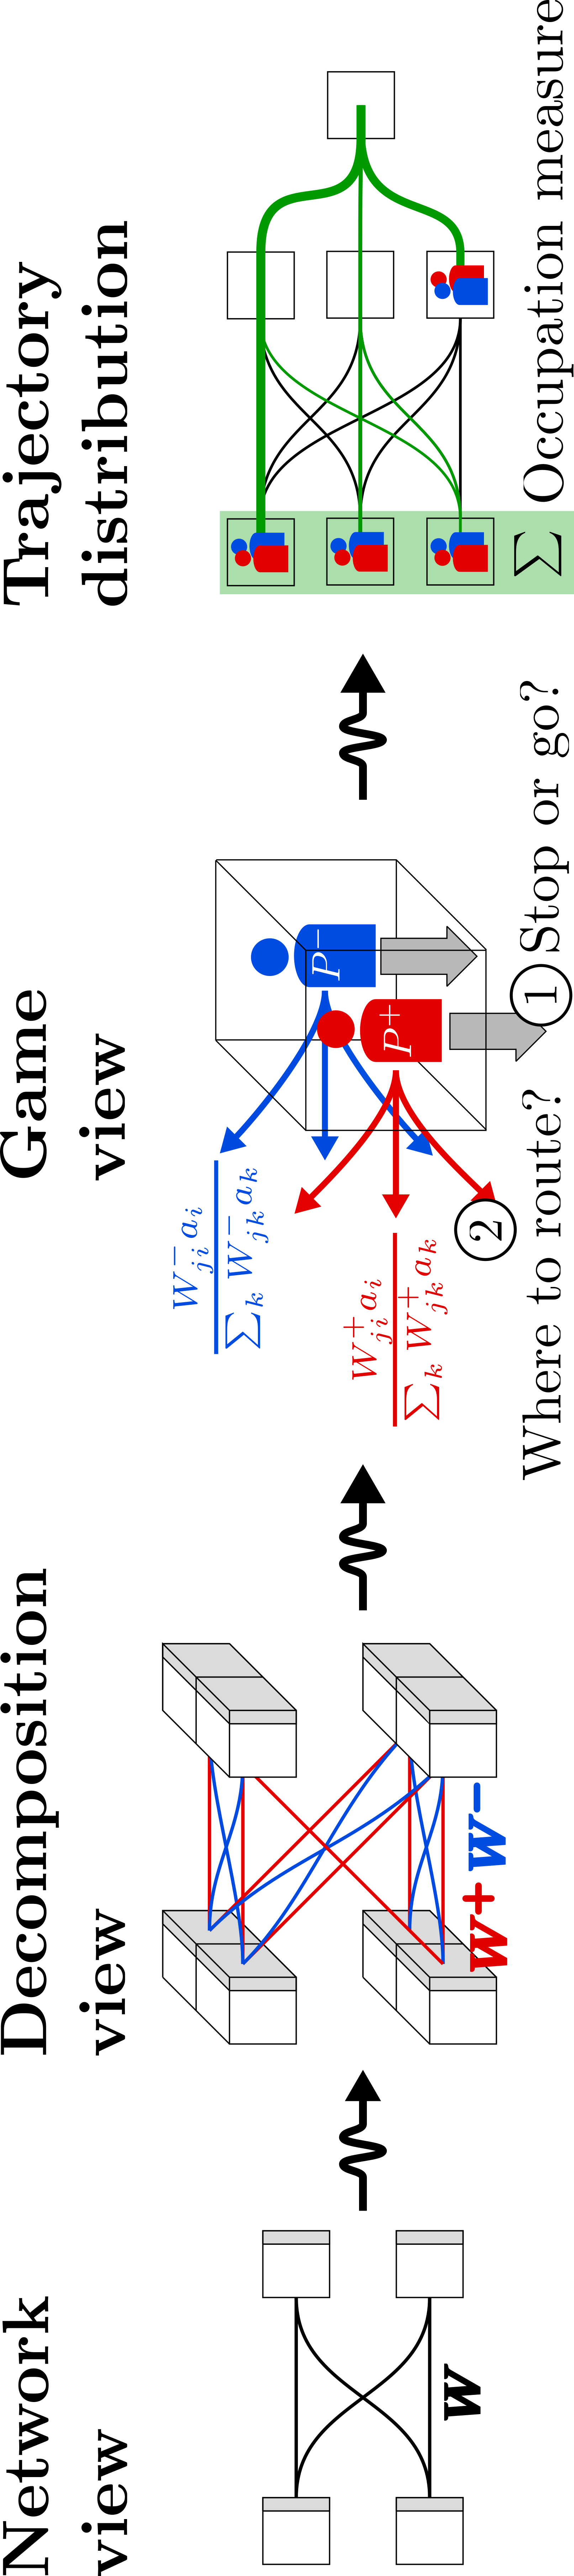
\includegraphics[angle=270,width=0.86\textwidth]{figures/ptnb_v2/main_figure.png}
\caption[The backward pass as a two-player game]{The backward pass as a two-player game. The Stopping Decomposition splits every weight by
sign, $W = W^+ - W^-$; at each state of the extended graph the players decide (1) stop or continue
and (2) where to route. Their equilibrium policies induce a distribution over backward
trajectories, and its signed discounted occupation measures at the input states recover the
attribution map.}
\label{fig:game_trajectory_overview}
\end{figure}

Oversight depends on the reliability of the evidence it uses. Parameter insensitivity, input dependence, perturbation fragility, and misleading modified-gradient structure~\parencite{Adebayo2018sanity,Kindermans2018PatternAttribution,Ghorbani2019fragile,Nie2018guided} can give false assurance about a model's visual dependencies. The two papers address complementary parts of this problem: the split representation exposes internal contributions and their derivative identities, while the game representation makes routing choices and distributions over calculations explicit. Numerical stabilization enables the former at depth; policy regularization, risk aversion, and extended action sets provide design choices for the latter. Hellinger diagnostics compare the resulting trajectory laws, complementing comparisons of their projected attribution maps. The experiments assess properties of these attribution methods; whether their use improves oversight or supports safer deployment remains a further empirical question.

Three research questions organize this combined account. \emph{What structure can be exposed without changing the network's function?} The decomposition framework connects monotone convex streams, sign-separated paths, and the polyhedral geometry of attainable gradients. \emph{What does a backward attribution actually calculate?} Derivative identities and game occupation measures relate local propagation rules to explicit global objects. \emph{How can these calculations support reliable inspection of vision models?} Stable implementations, controlled modifications of backward rules, and complementary evaluation criteria provide a basis for assessing what an attribution reveals and where its limitations lie.

\paragraph{Publication basis.}
This thesis brings together and extends two research works on which the thesis author is first author:
\begin{itemize}
    \item \emph{Hidden Monotonicity: Explaining Deep Neural Networks via their DC Decomposition}, coauthored with Georg Loho, was published at \textbf{CVPR 2026 and selected as a Highlight}~\parencite{hiddenMono}.\footnote{Official CVPR listing: \url{https://cvpr.thecvf.com/virtual/2026/poster/36564}.}
    \item \emph{Playing the Network Backward: A Game-Theoretic Attribution Framework}, coauthored with Jim Berend, Georg Loho, Sebastian Lapuschkin, and Wojciech Samek, is a \textbf{preprint}; this thesis uses arXiv:2605.06212v2, revised for AISTATS~\parencite{playingBackward2026}.
\end{itemize}
Their results are organized by the shared chain of questions: representation, backward semantics, method design, and evaluation. The experiments from each work remain separately identifiable. The thesis reuses their model-evaluation outputs, describes the implemented protocols, and recomputes the VOC uncertainty estimates with images as the resampling unit. It adds a common exposition of the decompositions, further mathematical connections, and a partial Lean formalization; Appendix~\ref{app:publication_provenance} records publication provenance and tool use.


\paragraph{Author's contribution.}
My principal contributions to the two underlying papers were developing the
theory, developing and conducting the experiments, and writing all appendices
and most of the paper text outside the introductions. These contributions were developed in
collaboration with the coauthors listed above. Appendix~\ref{app:author_contribution}
distinguishes this work from the subsequent integration and formalization in
the thesis.

\section{Contributions of This Thesis}\label{sec:contributions}

The contributions of this thesis are the following.

\begin{enumerate}
    \item \textbf{A general framework of network decompositions.}
    Chapter~\ref{ch:decompositions} introduces a \emph{network decomposition} and its \emph{validity}: a lift of a network into a pair of non-negative streams, propagated by non-negative maps $\Wsig{l}{+}, \Wsig{l}{-}$ and pairwise activations, whose difference recovers the original computation at every layer. Within it the thesis constructs a whole family --- the mixing family $\fmix$ interpolating between maximum- and minimum-based pair activations, the stopping decomposition $\fstop$, and regularized decompositions $\freg$ whose entropy-regularized member $\fsoft$ yields sigmoid-gated soft splits. The classical \ac{dc} split $f = g - h$ is the $\eta = 1$ endpoint of the mixing family rather than an isolated trick, and a splitting theorem for activations with integrable curvature extends the construction beyond \ac{relu} to GELU, Swish, tanh, sigmoid, and softplus networks.

    \item \textbf{A numerically stable \ac{dc} decomposition of \ac{relu} networks and \acp{cnn}.}
    A naive split can grow rapidly with depth while its difference stays bounded, so floating-point cancellation destroys the signal. Chapter~\ref{ch:decompositions} develops stabilization through transformations of the split activations and propagated signals. The exact convex representation extends to convolutions, convexity-preserving max-pooling, average pooling, fixed-statistic batch normalization, residual connections, and fixed dropout masks. The evaluated implementation additionally uses input-dependent recentering, cache correction, and optional winner-takes-it-all pooling. These procedures target forward reconstruction and usable backward signals; the individual stabilized streams do not inherit all convexity and monotonicity guarantees of the original representation.

    \item \textbf{A game-theoretic reformulation of the backward pass.}
    Chapter~\ref{ch:game_theory} reinterprets the stopping decomposition as a two-player zero-sum stopping game on an extended network graph, adapting the ReLU Net Game of \textcite{Gaubert2025}: layers are rounds, neurons states, sign switches hand the turn to the opponent, and the network output is the game value. Backward attribution is represented by \emph{signed discounted occupation measures over game trajectories}: propagation rules are equilibrium policies of the players $P^+$ and $P^-$, and attribution maps discounted occupation measures of that distribution. Two games anchor the theory --- the \ac{sg}, whose occupation measures recover the Jacobian, and the entropy-regularized \ac{rg}, recovering the full $\alpha\beta$-\ac{lrp} family --- giving the two methods a shared trajectory-space representation. These are representation theorems: the architecture alone does not determine a unique game or discount. The trajectory-space view of Chapter~\ref{ch:trajectory} further yields a Hellinger distance between normalized backward \emph{routing laws}, detecting routing changes that pixel-space sanity checks \parencite{Adebayo2018sanity} may obscure, and analytical \emph{modes} --- risk aversion, action-space augmentation, policy regularization --- mapping back to principled backpropagation rules.

    \item \textbf{New attribution methods and benchmark evaluations.}
    Chapter~\ref{ch:saliency} builds three attribution methods on the split representation: SplitCAM, a LayerCAM-inspired \parencite{Jiang2021LayerCAM} \ac{cam} method on the split-streams; SplitLRP, an adaptation of \ac{lrp} \parencite{Bach2015} to the split-pair; and SplitGrad, a gradient method exploiting the improved signal flow. Evaluated with the Quantus suite \parencite{Hedstrom2023} on VGG-16 \parencite{Simonyan2015} and ResNet-18 \parencite{He2016resnet} over ImageNet-S \parencite{Gao2022imagenets}, they show configuration-dependent gains in localization and Selectivity, with trade-offs in Pixel Flipping and robustness (Chapter~\ref{ch:experiments}). On ResNet-18, Guided Grad-CAM retains the highest reported Attribution Localization, and SplitCAM's Selectivity advantage over Guided Backprop is $0.014$. The chapter also develops directly trained difference-of-convex input neural networks and evaluates their stream sensitivities on MNIST (Section~\ref{sec:dcinns}).


    \item \textbf{A tropical-geometric interpretation and Imaginative Polytopes.}
    The tropical foundations (Section~\ref{sec:tropical_polyhedra_foundations}) place the decomposition in the polyhedral-geometry view of \ac{relu} networks \parencite{Zhang2018,Misiakos2022}: the split-streams $g$ and $h$ are the two tropical polynomials whose difference the network computes, their Newton polytopes evolving across layers by Minkowski sums and convex hulls. The thesis introduces \emph{Imaginative Polytopes} and proves that their vertices encode the attainable gradients of the split-streams, giving them an interpretation as learned visual prototypes and counterfactual feature profiles.

    \item \textbf{Extension to attention mechanisms and Transformers.}
    Chapter~\ref{ch:transformers} gives a recursive DC construction for deterministic Transformers of arbitrary finite depth, including signed attention projections, exact softmax, and LayerNorm with positive epsilon. Its streams are convex and monotone on non-negative doubled inputs and recover the full forward map exactly; numerical stability remains a separate issue. A distinct oracle-player construction treats the realized QK-softmax as a reference policy for conditioned Value routing. On ViT-B/16 \parencite{Dosovitskiy2021vit}, a selected game-derived attribution mode improves localization, with the selected configuration also evaluated on Pascal VOC without re-tuning. Pointing Game, Top-$k$ overlap, faithfulness, and robustness reveal distinct trade-offs; the revised evaluation reports independently validation-selected localization and faithfulness configurations, confidence intervals, and paired tests. These empirical results concern conditioned attribution, not the new full Transformer DC algorithm.
\end{enumerate}

\section{Positioning within the Literature}\label{sec:related_work}

This section positions the thesis along its three research questions; it is brief, since dedicated related-work discussions open the chapters where the material is developed --- games and propagation rules in Section~\ref{sec:related_work_games} and transformer interpretability in Section~\ref{sec:related_work_transformers}.

\paragraph{What structure is hidden inside a trained network?}
The idea that sign-constrained networks are the interpretable core of deep learning runs from monotonic networks \parencite{Sill1997_MonotonicNetworks,Daniels2010_MonotoneNN} through certified and lattice-based monotone models \parencite{Liu2020CertifiedMonotone,Gupta2016MonotoneLattice,Sivaraman2020_COMET,Nguyen2023_MonoNet,Runje_2023} to \acp{icnn} \parencite{Amos2017} and convex network calculus \parencite{Bach2017ConvexNN,Calafiore2019DLSE,sivaprasad2021curious}. \ac{dc} decompositions bridge this to unconstrained networks: classical \ac{dc} programming \parencite{Tao1997_DCProgramming,LeThi2018DCA,Sriperumbudur2009CCCP} and the representation theory of piecewise-linear functions as differences of convex ones \parencite{Melzer1986_PLasDC,Kripfganz1987_PWAasDC,Zalgaller2000_DCRepresentation,Griewank2020_PolyhedralDCDecomposition,Schlueter2021_ConvexDecompPAF,Koutschan2024_MinimalArity,Kazda2024_LP_DCPLA,Brandenburg2025_DecompositionPolyhedra} guarantee the split exists; \textcite{Awasthi2023DCNN} and \textcite{Siahkamari2020_DCRegression} construct essentially the split used here, for training and regression, and CDiNN-type architectures make the difference structure trainable \parencite{Sankaranarayanan2021CDINN,Chen2025_RCDiNN}. None confronts the numerical instability of the split or applies it to explanation, where this thesis departs. The geometric reading rests on the identification of \ac{relu} networks with \ac{cpwl} maps and tropical rational functions \parencite{Arora2018,Zhang2018,BalestrieroBaraniuk2018MadMax,Montufar2022,Misiakos2022,phuong2020functional,Hertrich2023,huchette2025deeplearningmeetspolyhedral}; the Newton-polytope perspective is developed in Section~\ref{sec:tropical_polyhedra_foundations}.

\paragraph{When can explanations be trusted?}
The attribution toolbox spans gradient saliency \parencite{Simonyan2014}, deconvolution and guided backpropagation \parencite{ZeilerFergus2014,Springenberg2015}, \ac{lrp} and Deep Taylor decomposition \parencite{Bach2015,Montavon2017DeepTaylor,Montavon2018}, \ac{cam} variants \parencite{Selvaraju2017,Chattopadhay2018,Jiang2021LayerCAM}, axiomatic methods \parencite{Sundararajan2017,Shrikumar2017}, noise averaging \parencite{Smilkov2017}, and perturbation- or surrogate-based explanations \parencite{Ribeiro2016,FongVedaldi2017,LundbergLee2017,Kolek2023_ShearletX,Fel2023_EVA}. A wave of critiques sharpened the trust question: sanity checks reveal parameter insensitivity \parencite{Adebayo2018sanity}, explanations can be fragile or manipulable \parencite{Ghorbani2019fragile,Dombrowski2019ManipulatedExplanations,AlvarezMelis2018robustness}, modified backward rules can produce structure unrelated to the model \parencite{Nie2018guided,sixt2020whenexplanationslie}, and input dependence confounds attribution \parencite{Kindermans2018PatternAttribution}. In response, evaluation frameworks such as Quantus \parencite{Hedstrom2023} operationalize faithfulness, localization \parencite{Zhang2018pointinggame}, robustness, and complexity \parencite{Bhatt2020complexity,Yeh2019} as measurable desiderata --- the standard this thesis holds its methods to in Chapter~\ref{ch:experiments}. The thesis' answer is structural rather than post hoc: attribution is computed on a representation (the split-pair) in which evidence cannot cancel invisibly, or derived from a game whose trajectory distribution records normalized backward routing and whose signed discounted occupation measures recover attribution, so sanity-check failures can be studied at both the trajectory and pixel levels (Chapter~\ref{ch:trajectory}); their different responses to randomization do not by themselves establish explanation faithfulness.

\paragraph{How can attribution be made stable?}
The closest precursor to the game framework is the ReLU Net Game of \textcite{Gaubert2025}, which identifies forward evaluation with the value of a zero-sum stopping game but connects it neither to the backward pass nor to attribution. Related stochastic views of relevance flow include Excitation Backprop's absorbing Markov chain \parencite{Zhang2018pointinggame}, which the \ac{sg} generalizes by adding an opponent, and the \ac{nrm} framework \parencite{Xiong2026nrm}, a signed-measure calculus over walks compared with our trajectory distributions in Section~\ref{sec:nrm_comparison}. Shapley-value methods \parencite{LundbergLee2017} play a \emph{different}, cooperative game over input coalitions in a black-box setting, complementary to the white-box backward game here. Stability itself has been approached via curvature reduction with softplus activations \parencite{Dombrowski2020} --- recovered here as entropy regularization of the stop decision --- and via risk-sensitive control \parencite{zhang2021risk} motivating the risk-averse game modes. On transformers, attention rollout and flow \parencite{Abnar2020attention}, transformer-\ac{lrp} \parencite{Chefer2021ICCV,Chefer2021GenericAttention,Ali2022AttnLRP,Achtibat2024AttnLRP}, and artifact-aware constructions \parencite{Wrobel2024,darcet2024vision} define the state of the art Chapter~\ref{ch:transformers} engages with; Section~\ref{sec:related_work_games} and Section~\ref{sec:related_work_transformers} give the full accounts. For visual inspection and attribution-guided correction~\parencite{Pahde2023R2R}, instability can obscure unwanted dependencies and misdirect subsequent interventions.

\paragraph{Outline.}
Chapter~\ref{ch:foundations} assembles the foundations: network notation, \ac{cpwl} mappings, convexity and monotonicity, \acp{mdp} and zero-sum games --- including the ReLU Net Game of Gaubert and Vlassopoulos --- and the tropical geometry of the split with the Imaginative-Polytope picture. Chapter~\ref{ch:decompositions} develops the decomposition framework, the smooth-activation splitting theorem, numerical stabilization, and the \ac{cnn} extension; Chapter~\ref{ch:game_theory} the two-player stopping and routing games, with gradients and $\alpha\beta$-\ac{lrp} recovered as equilibrium occupation measures; Chapter~\ref{ch:transformers} the extension and implementation on multiplicative operations and \acp{vit}; and Chapter~\ref{ch:saliency} the split methods SplitCAM, SplitLRP, and SplitGrad, inherently interpretable difference-of-convex architectures, and the attribution modes. Chapter~\ref{ch:experiments} reports the evaluation on ImageNet-S and Pascal VOC across VGG-16, ResNet, and ViT-B/16; Chapter~\ref{ch:trajectory} develops the trajectory-distribution view and its Hellinger diagnostics; and Chapter~\ref{ch:conclusion} concludes with future directions from \acp{llm} to hardware-level acceleration.

\chapter{Mathematical Foundations}\label{ch:foundations}

This chapter establishes the notation and background. Section~\ref{sec:nn_notation_pwl} introduces feedforward networks and their \ac{relu}--\ac{cpwl} equivalence. Section~\ref{sec:convex_monotone_foundations} defines monotone networks, \acp{icnn}, and Maxout units, the building blocks of Chapter~\ref{ch:decompositions}. Section~\ref{sec:game_theory_mdp_foundations} presents \acp{mdp}, zero-sum turn-based games, and the full ReLU Net Game of Gaubert and Vlassopoulos, distinguishing the framework inherited by Chapter~\ref{ch:game_theory} from its extensions. The absolute-curvature construction for smooth activations accompanies the network decomposition theorem in Section~\ref{sec:dc_splitting_smooth}.

\section{Neural Network Notation and PWL Mappings}\label{sec:nn_notation_pwl}

The standard feedforward architecture serves as the reference model throughout; convolutional and attention-based architectures are treated in Section~\ref{sec:cnn_decompositions} and Chapter~\ref{ch:transformers} as structured special cases and extensions.

\begin{definition}[Feedforward \ac{relu} network]\label{def:ffn_relu}
Let $L \in \NN$ and let $d^{(0)}, d^{(1)}, \ldots, d^{(L)} \in \NN$ denote the \emph{layer widths}, with input dimension $d^{(0)}$ and output dimension $d^{(L)}$. A \emph{feedforward \ac{relu} network} of depth $L$ is given by weight matrices $\Wl{l} \in \RR^{d^{(l)} \times d^{(l-1)}}$ and bias vectors $b^{(l)} \in \RR^{d^{(l)}}$ for $l = 1, \ldots, L$. On an input $x \in \RR^{d^{(0)}}$ it computes the recursion
\begin{align}
	\actl{0} &\coloneqq x, \notag\\
	\preactl{l} &\coloneqq \Wl{l} \actl{l-1} + b^{(l)}, && l = 1, \ldots, L, \label{eq:forward_recursion}\\
	\actl{l} &\coloneqq \relu\bigl(\preactl{l}\bigr), && l = 1, \ldots, L-1, \notag
\end{align}
where $\relu(z) \coloneqq \max\{z, 0\}$ acts componentwise, and the output layer is affine, $\actl{L} \coloneqq \preactl{L}$. We call $\preactl{l}$ the \emph{pre-activation} and $\actl{l}$ the \emph{(post-)activation} of layer $l$, and denote the \emph{network function} by
\begin{equation}
	f \colon \RR^{d^{(0)}} \longrightarrow \RR^{d^{(L)}},
	\qquad
	f(x) \coloneqq \actl{L}.
	\label{eq:network_function}
\end{equation}
Layers $1, \ldots, L-1$ are the \emph{hidden layers}. Throughout we fix the boundary convention $\relu'(0) \coloneqq 0$, so that the gate indicator $\1\{\preactl{l}_i > 0\}$ returns $0$ at $\preactl{l}_i = 0$.
\end{definition}

For layers $l, \ldots, L$, write $f^{(l)} \colon \RR^{d^{(l)}} \to \RR^{d^{(L)}}$ for the tail map, with $f = f^{(1)} \circ \bigl(x \mapsto \relu(\Wl{1} x + b^{(1)})\bigr)$ and $f^{(L)}$ the affine output map. Appending a constant \emph{intercept input} $1$ absorbs $b^{(l)}$ into a column of $\Wl{l}$; some proofs use this bias-free formulation implicitly.

Chapter~\ref{ch:decompositions} splits parameters and inputs by sign using the following notation.

\begin{definition}[Positive and negative parts]\label{def:posneg_parts}
For a scalar $u \in \RR$ we write $u^{+} \coloneqq \max\{u, 0\}$ and $u^{-} \coloneqq \max\{-u, 0\}$, so that $u = u^{+} - u^{-}$ and $\abs{u} = u^{+} + u^{-}$, with $u^+ u^- = 0$. For a matrix or vector $W$ and a sign label $\sigma \in \{+,-\}$, the \emph{entrywise part} $\posneg{W}{\sigma}$ is obtained by applying $u \mapsto u^{\sigma}$ to every entry. For the layer weights and biases of Definition~\ref{def:ffn_relu} we abbreviate
\begin{equation}
	\Wsig{l}{\sigma} \coloneqq \posneg{\Wl{l}}{\sigma},
	\qquad
	b^{(l,\sigma)} \coloneqq \posneg{b^{(l)}}{\sigma},
	\qquad \sigma \in \{+,-\},
	\label{eq:weight_split}
\end{equation}
so that $\Wl{l} = \Wsig{l}{+} - \Wsig{l}{-}$ and $\abs{\Wl{l}} = \Wsig{l}{+} + \Wsig{l}{-}$ entrywise, and both $\Wsig{l}{\sigma}$ are entrywise non-negative.
\end{definition}

\begin{remark}[Pair notation for decomposed activations]\label{rem:pair_notation}
The activation labels $\act{l}{\sigma}$, $\sigma \in \{+,-\}$, denote the two non-negative \emph{streams} defined in Section~\ref{sec:general_decomposition_def}, distinct from the entrywise parts $\posneg{\actl{l}}{\sigma}$. The streams carry strictly more information than the sign pattern of $\actl{l}$, supplying the sub-threshold signals exploited in Chapter~\ref{ch:saliency}.
\end{remark}

\subsection*{Continuous piecewise linear functions}

The function class computed by \ac{relu} networks admits an exact geometric description.

\begin{definition}[\ac{cpwl} function]\label{def:cpwl}
A function $f \colon \RR^{d} \to \RR^{m}$ is \emph{\acl{cpwl}} (\acs{cpwl}) if it is continuous and there exist finitely many closed polyhedra $Q_1, \ldots, Q_N \subseteq \RR^d$ with $\bigcup_{r=1}^{N} Q_r = \RR^d$ such that the restriction of $f$ to each $Q_r$ is an affine map. The full-dimensional polyhedra on which $f$ is affine, taken maximal with respect to inclusion, are called the \emph{linear regions} of $f$.
\end{definition}

For example, $\abs{\cdot} \colon \RR \to \RR$ is \ac{cpwl} with the two regions $(-\infty, 0]$ and $[0, \infty)$, and $x \mapsto \max\{x_1, \ldots, x_d\}$ is \ac{cpwl} with $d$ regions.

\begin{observation}[\LeanResult{obs:relu_is_cpwl}]\label{obs:relu_is_cpwl}
Every feedforward \ac{relu} network represents a \ac{cpwl} function.\end{observation}

\begin{proof}
Affine maps and componentwise $\relu$ are \ac{cpwl}. Composition preserves this class: if $f$ and $g$ are affine on polyhedral covers $Q_1, \ldots, Q_N$ and $P_1, \ldots, P_M$ of their respective domains, then $g\circ f$ is affine on the cover of at most $NM$ polyhedra $Q_r\cap f^{-1}(P_s)$. These are polyhedra because $f$ is affine on each $Q_r$; composition also preserves continuity. Induction along \eqref{eq:forward_recursion} proves the claim.
\end{proof}

Conversely, every \ac{cpwl} function has an exact \ac{relu} representation with a dimension-dependent depth bound \parencite{Arora2018}. This equivalence underlies the difference-of-convex analysis of Chapter~\ref{ch:decompositions}.

\begin{theoremenv}[\ac{cpwl}--\ac{relu} equivalence, \parencite{Arora2018}, \LeanResult{thm:cpwl_relu_equivalence}]\label{thm:cpwl_relu_equivalence}
A function $f \colon \RR^{d} \to \RR$ is \ac{cpwl} if and only if it is representable by a feedforward \ac{relu} network. Moreover, every \ac{cpwl} function on $\RR^d$ is representable by a \ac{relu} network of depth at most $\bigl\lceil \log_2(d+1) \bigr\rceil + 1$.\end{theoremenv}

\begin{proof}
Observation~\ref{obs:relu_is_cpwl} proves the ``if'' direction. For the converse, every \ac{cpwl} function $f$ admits a \emph{difference-of-convex} representation
\begin{equation}
	f = g - h,
	\qquad
	g = \max_{r \in [N_g]}\, \ell_r,
	\qquad
	h = \max_{s \in [N_h]}\, m_s,
	\label{eq:cpwl_dc_representation}
\end{equation}
with finitely many affine functions $\ell_r, m_s \colon \RR^d \to \RR$ \parencite{Melzer1986_PLasDC,Kripfganz1987_PWAasDC}; their finite maxima $g,h$ are convex. The maximum of two scalars is a two-layer \ac{relu} computation,
\begin{equation}
	\max\{u, v\}
	= \frac{u + v}{2} + \frac{\abs{u - v}}{2}
	= \frac{u + v}{2} + \frac{\relu(u - v) + \relu(v - u)}{2},
	\label{eq:max_as_relu}
\end{equation}
absorbing the affine pre- and post-combinations into surrounding weight matrices. A balanced binary tree of pairwise maxima realizes $g$ at depth $\lceil \log_2 N_g \rceil + 1$, and likewise $h$; a final affine layer forms \eqref{eq:cpwl_dc_representation}, proving representability. For the bound independent of the number of pieces, \textcite{Arora2018} use the Wang--Sun representation of every \ac{cpwl} function on $\RR^d$ as a signed sum of maxima of at most $d+1$ affine functions each. These need at most $\lceil \log_2(d+1) \rceil$ hidden layers and a final affine output layer.
\end{proof}

\begin{remark}[Expressivity and linear regions]\label{rem:linear_regions}
Theorem~\ref{thm:cpwl_relu_equivalence} identifies the function \emph{class}, not the \emph{cost} of representation: deep networks can represent \ac{cpwl} functions with exponentially many linear regions in the number of neurons, an interplay of depth, width, and region counts surveyed by \textcite{huchette2025deeplearningmeetspolyhedral}. The representation \eqref{eq:cpwl_dc_representation} also foreshadows the central theme of this thesis: the convex \ac{cpwl} streams $g$ and $h$ of the DC split can be extracted \emph{constructively and locally} from a trained network, the subject of Section~\ref{sec:dc_splitting_relu}. For a stream $g(x)=\max_r(a_r^\top x+b_r)$, a uniquely active affine piece gives $\nabla g(x)=a_r$: the stream gradient records the slope of its current linear region.
\end{remark}

\section{Convexity and Monotonicity in Neural Networks}\label{sec:convex_monotone_foundations}

Chapter~\ref{ch:decompositions} splits general networks into sign-constrained components. We define the two classes and prove their monotonicity and convexity, respectively.

We order $\RR^d$ coordinatewise: $x \le y$ if and only if $x_i \le y_i$ for all $i \in [d]$. A function $f \colon \RR^d \to \RR^m$ is \emph{monotone} (non-decreasing) if $x \le y$ implies $f(x) \le f(y)$.

\begin{definition}[Monotone neural network]\label{def:monotone_network}
A feedforward network with recursion \eqref{eq:forward_recursion} and monotone activation functions is called a \emph{monotone neural network} if all its weight matrices are entrywise non-negative, $\Wl{l} \ge 0$ for all $l = 1, \ldots, L$.
\end{definition}

Weight-sign constraints are an established device for building monotone models \parencite{Sill1997_MonotonicNetworks,Daniels2010_MonotoneNN} and remain central to modern monotone architectures \parencite{Runje_2023}; monotonicity can also be certified without imposing such constraints \parencite{Liu2020CertifiedMonotone}.

\begin{proposition}[Monotone networks represent monotone functions, \LeanResult{prop:monotone_represents}]\label{prop:monotone_represents}
A monotone neural network represents a monotone function; each coordinate function is non-decreasing in every input variable.\end{proposition}

\begin{proof}
Induct from the monotone input $\actl{0}=x$. Non-negative weights preserve coordinatewise order: $a\le a'$ implies $\Wl{l}a+b^{(l)}\le\Wl{l}a'+b^{(l)}$. Thus monotonicity of $\actl{l-1}$ implies that of $\preactl{l}$; componentwise monotone activation gives monotonicity of $\actl{l}$. The same order argument covers the affine output.
\end{proof}

\begin{definition}[\acl{icnn}, \parencite{Amos2017}]\label{def:icnn}
A feedforward network with recursion \eqref{eq:forward_recursion} whose activation functions are convex \emph{and} monotone is called an \emph{\acl{icnn}} (\acs{icnn}) if all weight matrices except possibly the first are entrywise non-negative, $\Wl{l} \ge 0$ for all $l = 2, \ldots, L$, while $\Wl{1}$ is unconstrained.
\end{definition}

Definition~\ref{def:icnn} covers the plain feedforward core of the architecture of \textcite{Amos2017}; their sign-unconstrained skip (``passthrough'') connections do not affect the statement below, since they enter each pre-activation affinely in $x$.

\begin{proposition}[\acp{icnn} represent convex functions, \LeanResult{prop:icnn_convex}]\label{prop:icnn_convex}
An \ac{icnn} represents a convex function; each coordinate of every activation $\actl{l}$, $l \ge 1$, is a convex function of the input $x$.\end{proposition}

\begin{proof}
We use two closure properties of convex functions: (i) a non-negative linear combination of convex functions plus a constant is convex; (ii) if $\varphi \colon \RR \to \RR$ is convex and non-decreasing and $u \colon \RR^d \to \RR$ is convex, then $\varphi \circ u$ is convex, since for $\lambda \in [0,1]$,
\begin{equation*}
	\varphi\bigl(u(\lambda x + (1-\lambda) y)\bigr)
	\le \varphi\bigl(\lambda u(x) + (1-\lambda) u(y)\bigr)
	\le \lambda\, \varphi(u(x)) + (1-\lambda)\, \varphi(u(y)),
\end{equation*}
where the first inequality uses convexity of $u$ and monotonicity of $\varphi$, and the second convexity of $\varphi$.

Induct over layers. The affine coordinates of $\preactl{1}=\Wl{1}x+b^{(1)}$ are convex, so (ii) gives convexity of $\actl{1}$. If $\actl{l-1}$ has convex coordinates, the non-negative weights for $l\ge2$ make $\preactl{l}=\Wl{l}\actl{l-1}+b^{(l)}$ convex by (i), and (ii) preserves convexity through the activation. The identity activation covers the affine output $\actl{L}=\preactl{L}$.
\end{proof}

\begin{remark}[Monotonicity and convexity combine]\label{rem:monotone_convex_combined}
If, in addition, $\Wl{1} \ge 0$ in Definition~\ref{def:icnn}, the network is simultaneously monotone and input-convex, hence non-decreasing \emph{and} convex by Propositions~\ref{prop:monotone_represents} and \ref{prop:icnn_convex}. Both $\relu$ and Maxout (below) are convex and monotone, so non-negative-weight \ac{relu} networks are of exactly this type. These are the building blocks of the DC splitting of Section~\ref{sec:dc_splitting_relu}: the streams $g$ and $h$ are computed by monotone networks acting on a signed embedding of the input, and are input-convex in the original input. The sign constraint also \emph{limits} expressivity---a weight-constrained \ac{relu} network represents only convex functions, precisely Proposition~\ref{prop:icnn_convex}, which is why monotone architectures add concave counterparts of the activation \parencite{Runje_2023}. The decompositions of this thesis turn the limitation into a feature: the difference of two such networks recovers full generality by Theorem~\ref{thm:cpwl_relu_equivalence} and \eqref{eq:cpwl_dc_representation}.
\end{remark}

\subsection*{Maxout units}

\begin{definition}[Maxout unit and Maxout network, \parencite{Goodfellow2013Maxout}]\label{def:maxout}
A \emph{rank-$k$ Maxout unit} with weights $w_1, \ldots, w_k \in \RR^{d}$ and biases $\beta_1, \ldots, \beta_k \in \RR$ computes
\begin{equation}
	x \longmapsto \maxout(x) \coloneqq \max_{j \in [k]} \bigl( w_j^{\top} x + \beta_j \bigr).
	\label{eq:maxout_unit}
\end{equation}
A \emph{rank-$k$ Maxout network} is a feedforward network whose neurons are rank-$k$ Maxout units; equivalently, layer $l$ carries $k$ weight matrices $W^{(l)}_1, \ldots, W^{(l)}_k$ and biases $b^{(l)}_1, \ldots, b^{(l)}_k$, and
\begin{equation}
	\actl{l}_i \coloneqq \max_{j \in [k]} \bigl( W^{(l)}_j \actl{l-1} + b^{(l)}_j \bigr)_i .
	\label{eq:maxout_layer}
\end{equation}
\end{definition}

\begin{observation}[\ac{relu} and max-pooling as Maxout, \LeanResult{obs:relu_maxout_special_case}]\label{obs:relu_maxout_special_case}
The \ac{relu} activation is the rank-$2$ Maxout unit with parameters $(w_1, \beta_1) = (w, \beta)$ and $(w_2, \beta_2) = (0, 0)$, since $\relu(w^\top x + \beta) = \max\{w^\top x + \beta,\, 0\}$. Max-pooling over a group $J$ of neurons is the rank-$\abs{J}$ Maxout unit whose $j$-th argument is the coordinate projection onto the $j$-th element of $J$. Every rank-$k$ Maxout unit is convex in its input and non-decreasing in each pre-activation argument $w_j^\top x + \beta_j$; hence Maxout qualifies as an admissible activation in Definitions~\ref{def:monotone_network} and \ref{def:icnn}.\end{observation}

\begin{proof}
The first two claims follow from \eqref{eq:maxout_unit}. A maximum of affine functions is convex. For argument-wise monotonicity, set $u_j=w_j^\top x+\beta_j$: $u_j\le u_j'$ for all $j$ implies $\max_j u_j\le\max_j u_j'$.
\end{proof}

\begin{remark}\label{rem:maxout_role}
Maxout networks are the natural piecewise-linear generalization of \ac{relu}: a rank-$k$ unit expresses a maximum of $k$ affine functions in one neuron, matching the building blocks of the DC representation \eqref{eq:cpwl_dc_representation}. The DC splitting of Chapter~\ref{ch:decompositions} is developed for \ac{relu} networks and extended to Maxout units---and to the multiplicative interactions needed for attention---in Chapter~\ref{ch:transformers}, using the exchange identity $\max_{j \in [k]}(u_j - v_j) = \max_{j \in [k]}\bigl\{ u_j + \sum_{i \ne j} v_i \bigr\} - \sum_{i \in [k]} v_i$ for pairs of non-negative streams.
\end{remark}

\section{Game Theory and Markov Decision Processes}\label{sec:game_theory_mdp_foundations}

Chapter~\ref{ch:game_theory} interprets backward propagation as a two-player zero-sum game on the decomposed network graph. We introduce \acp{mdp}, turn-based games, and their optimality equations, restricting throughout to finite state and action spaces.

\begin{definition}[\acl{mdp}]\label{def:mdp}
A (finite) \emph{\acl{mdp}} (\acs{mdp}) \parencite{Puterman1994mdp,SuttonBarto2018rl} is a tuple $\mathcal{M} = (S, A, \P, R, \gamma)$ consisting of a finite state set $S$, a finite action set $A(s)$ for each $s \in S$, a \emph{transition kernel} $\P(s' \mid s, a) \ge 0$ with $\sum_{s'} \P(s' \mid s, a) = 1$, a bounded \emph{reward function} $R(s, a) \in \RR$, and a \emph{discount factor} $\gamma \in [0, 1)$. A \emph{(stationary) policy} is a map $\pi$ assigning to each state $s$ a probability distribution $\pi(\cdot \mid s)$ over $A(s)$; $\pi$ is \emph{pure} (deterministic) if each $\pi(\cdot \mid s)$ is a point mass. A policy induces, for every start state, a Markov chain on $S$ and hence a distribution over trajectories $(s_0, a_0, s_1, a_1, \ldots)$; the \emph{value function} of $\pi$ is the expected discounted return
\begin{equation}
	V^{\pi}(s) \coloneqq \E^{\pi}\Bigl[ \textstyle\sum_{t=0}^{\infty} \gamma^{t}\, R(s_t, a_t) \,\Big|\, s_0 = s \Bigr],
	\label{eq:mdp_value}
\end{equation}
and the \emph{optimal value function} is $V^{\star}(s) \coloneqq \max_{\pi} V^{\pi}(s)$.
\end{definition}

Fixing an enumeration of $S$, a pure policy $\pi$ turns the kernel into a row-stochastic \emph{transition matrix} $P^{\pi} \in \RR^{S \times S}$ with $P^{\pi}_{s s'} = \P(s' \mid s, \pi(s))$ and the reward into a vector $R^{\pi}$, and \eqref{eq:mdp_value} becomes the Neumann series $V^{\pi} = \sum_{t \ge 0} \gamma^t (P^{\pi})^t R^{\pi}$. This matrix picture recurs in Chapter~\ref{ch:game_theory}, where the (sub)stochastic matrices are built from the normalized weight parts $\Wsig{l}{\sigma}$ of Definition~\ref{def:posneg_parts}.

\begin{proposition}[Bellman equations, \LeanResult{prop:bellman}]\label{prop:bellman}
Let $\mathcal{M}$ be a finite \ac{mdp} with $\gamma \in [0,1)$. Then:
\begin{enumerate}
	\item $V^{\pi}$ is the unique solution of the linear system
	\begin{equation}
		V(s) = \sum_{a \in A(s)} \pi(a \mid s) \Bigl[ R(s,a) + \gamma \sum_{s'} \P(s' \mid s, a)\, V(s') \Bigr],
		\qquad s \in S.
		\label{eq:bellman_evaluation}
	\end{equation}
	\item $V^{\star}$ is the unique solution of the \emph{Bellman optimality equation}
	\begin{equation}
		V(s) = \max_{a \in A(s)} \Bigl\{ R(s, a) + \gamma \sum_{s'} \P(s' \mid s, a)\, V(s') \Bigr\},
		\qquad s \in S,
		\label{eq:bellman_optimality}
	\end{equation}
	and any pure policy $\polstar$ that selects, in every state, an action attaining the maximum in \eqref{eq:bellman_optimality} is optimal: $V^{\polstar} = V^{\star}$.
\end{enumerate}\end{proposition}

\begin{proof}
Both claims are standard \parencite{Puterman1994mdp,SuttonBarto2018rl}. The right-hand sides of \eqref{eq:bellman_evaluation} and \eqref{eq:bellman_optimality} define $\gamma$-contractions on $\bigl(\RR^{S}, \norm{\cdot}_{\infty}\bigr)$, so each has a unique fixed point by the Banach fixed-point theorem; conditioning \eqref{eq:mdp_value} on the first transition identifies these fixed points as $V^{\pi}$ and $V^{\star}$, and any policy greedy for $V^{\star}$ is optimal. The acyclic games below make even the contraction argument unnecessary (Remark~\ref{rem:structural_discount}).
\end{proof}

\begin{remark}[State-dependent structural discounts]\label{rem:structural_discount}
Our games use \emph{state-dependent} discounts $\gamma(s)\ge0$ that may exceed $1$. These are \emph{structural} normalizers: for neuron $i$ in layer $l$, the absolute weight mass
\begin{equation}
	\gamma^{(l)}_i \coloneqq \sum_{j} \bigl( \Wsig{l}{+} + \Wsig{l}{-} \bigr)_{ij} = \sum_j \abs{\Wl{l}_{ij}},
	\label{eq:structural_discount}
\end{equation}
restores the mass after normalizing row $i$ of $\abs{\Wl{l}}$ into transition probabilities. Although contraction is unavailable, \emph{layered acyclic} graphs ensure finite trajectories and value sums. Backward induction gives a unique value and optimal policies, possibly nonunique at ties, as the two-player theorem below shows.
\end{remark}

\subsection*{Zero-sum turn-based games}

Two-player games enter because a decomposed network carries two interacting streams: a player $P^{+}$ who collects positive evidence and a player $P^{-}$ who collects negative evidence. We use the following conventions throughout: $p, q, r \in \{+, -\}$ denote player, turn, or sign labels; $\opp{p}$ denotes the opponent ($\opp{+} = -$, $\opp{-} = +$); the \emph{sign-XOR} $p \oplus q$ is $+$ if $p = q$ and $-$ otherwise; and $\xi_{p} \in \{+1, -1\}$ is the numerical sign of the label $p$, so that $\xi_{p}\, \xi_{q} = \xi_{p \oplus q}$.

\begin{definition}[Zero-sum turn-based game]\label{def:turn_based_game}
A (finite) \emph{zero-sum turn-based game} is a tuple $\mathcal{G} = (S_{+}, S_{-}, S_{\mathrm{ter}}, A, \P, R, \gamma)$ where the state set $S = S_{+} \uplus S_{-} \uplus S_{\mathrm{ter}}$ is partitioned into states controlled by player $P^{+}$, states controlled by player $P^{-}$, and terminal states; the action sets $A(s)$, the transition kernel $\P$, and the reward $R$ are as in Definition~\ref{def:mdp} on non-terminal states; $\gamma \colon S \to \RR_{\ge 0}$ is a (possibly state-dependent) discount; and each terminal state $s \in S_{\mathrm{ter}}$ carries a fixed one-time payoff $R(s)$. A \emph{policy pair} $\pi = (\pi_{+}, \pi_{-})$ consists of a policy $\pi_{p}$ for player $P^{p}$ on $S_{p}$. Play generates a trajectory as in an \ac{mdp}, with the player in turn choosing the action; the expected total payoff $V^{\pi}(s)$, defined as in \eqref{eq:mdp_value} with the discount accumulated multiplicatively along the trajectory ($\gamma^t$ replaced by $\prod_{m=0}^{t-1}\gamma(s_m)$), is paid \emph{by $P^{-}$ to $P^{+}$}: player $P^{+}$ maximizes $V^{\pi}$ and player $P^{-}$ minimizes it.
\end{definition}

\begin{theoremenv}[Shapley--Bellman optimality on layered games, \LeanResult{thm:shapley_bellman}]\label{thm:shapley_bellman}
Let $\mathcal{G}$ be a finite zero-sum turn-based game whose transition graph is acyclic. Then $\mathcal{G}$ has a \emph{value}: there is a unique function $V^{\star} \colon S \to \RR$ satisfying the \emph{Shapley--Bellman optimality equations}
\begin{equation}
	V^{\star}(s) =
	\begin{cases}
		\displaystyle \max_{a \in A(s)} \Bigl\{ R(s,a) + \gamma(s) \sum_{s'} \P(s' \mid s, a)\, V^{\star}(s') \Bigr\}, & s \in S_{+}, \\[1.2em]
		\displaystyle \min_{a \in A(s)} \Bigl\{ R(s,a) + \gamma(s) \sum_{s'} \P(s' \mid s, a)\, V^{\star}(s') \Bigr\}, & s \in S_{-}, \\[1.2em]
		R(s), & s \in S_{\mathrm{ter}},
	\end{cases}
	\label{eq:shapley_bellman}
\end{equation}
and there exist pure stationary policies $\polstar = (\polstar_{+}, \polstar_{-})$, obtained by selecting maximizing respectively minimizing actions in \eqref{eq:shapley_bellman}, such that for all $s \in S$ and all policies $\pi_{+}, \pi_{-}$,
\begin{equation}
	V^{(\polstar_{+}, \pi_{-})}(s) \;\ge\; V^{\polstar}(s) = V^{\star}(s) \;\ge\; V^{(\pi_{+}, \polstar_{-})}(s).
	\label{eq:saddle_point}
\end{equation}
In particular, $\polstar$ is a Nash equilibrium of every subgame, i.e.\ a subgame perfect equilibrium.\end{theoremenv}

\begin{proof}
Induct backward along a topological order of the finite acyclic graph. At terminal states, \eqref{eq:shapley_bellman} fixes $V^{\star}(s)=R(s)$ and \eqref{eq:saddle_point} holds. For $s\in S_+$, assume uniqueness and the saddle inequalities at all successors. Each action's bracket in \eqref{eq:shapley_bellman} is finite; maximizing over the finite action set uniquely defines $V^{\star}(s)$ and supplies a pure choice $\polstar_+(s)$. For any opponent policy $\pi_-$, condition on the first transition and apply the successors' left saddle inequality with $\gamma(s)\ge0$:
\begin{align*}
	V^{(\polstar_{+}, \pi_{-})}(s)
	&= R\bigl(s, \polstar_{+}(s)\bigr) + \gamma(s) \sum_{s'} \P\bigl(s' \mid s, \polstar_{+}(s)\bigr)\, V^{(\polstar_{+}, \pi_{-})}(s') \\
	&\ge R\bigl(s, \polstar_{+}(s)\bigr) + \gamma(s) \sum_{s'} \P\bigl(s' \mid s, \polstar_{+}(s)\bigr)\, V^{\star}(s')
	\;=\; V^{\star}(s),
\end{align*}
The last equality uses the maximizing choice $\polstar_+(s)$. Against $\polstar_-$, any $\pi_+$ averages the bracket to at most its maximum; conditioning and the successors' right saddle inequality give $V^{(\pi_+,\polstar_-)}(s)\le V^{\star}(s)$. For $s\in S_-$, exchange $\max$ with $\min$ and reverse the inequalities. Taking $\pi=\polstar$ in both inequalities gives $V^{\polstar}=V^{\star}$. The argument holds in every rooted subgame, proving subgame perfection.
\end{proof}

\begin{remark}\label{rem:shapley_history}
For general discounted stochastic games with cycles, existence of the value and of optimal stationary policies is Shapley's theorem \parencite{Shapley1953stochastic}, proved by the contraction argument of Proposition~\ref{prop:bellman} applied to the \emph{Shapley operator}---the min-max analogue of the Bellman operator \eqref{eq:shapley_bellman}. \textcite{Gaubert2025} formulate their network games in this operator language. The layered acyclic case of Theorem~\ref{thm:shapley_bellman} is all we need, and it additionally delivers subgame perfection, on which Chapter~\ref{ch:trajectory} relies.
\end{remark}

\subsection{The ReLU Net Game of Gaubert and Vlassopoulos}\label{subsec:relu_net_game}

\textcite{Gaubert2025} represent the forward pass of a \ac{relu} network as the value of a zero-sum turn-based stopping game played backward on its graph. We give their full construction in our notation; Chapter~\ref{ch:game_theory} retains its states, transitions, and stopping structure with revised payoff bookkeeping. Fix a network from Definition~\ref{def:ffn_relu} with scalar output ($d^{(L)}=1$), an input $x\in\RR^{d^{(0)}}$, and nonzero weight rows, ensuring strictly positive discounts \eqref{eq:structural_discount}.

Read the identity $\actl{l}_i = \max\bigl\{0,\, \preactl{l}_i\bigr\}$ as a decision: a player at neuron $i$ may \emph{stop}, securing payoff $0$, or \emph{continue}, collecting the bias $b^{(l)}_i$ plus the weighted contributions of the previous layer. Continuing propagates the decision backward through the network; a negative weight flips the sign of its contribution, i.e.\ hands the turn to an adversary facing the mirrored problem. The optimal value at neuron $i$ is exactly the activation $\actl{l}_i$.

\begin{definition}[ReLU Net Game, following \parencite{Gaubert2025}]\label{def:relu_net_game}
The \emph{ReLU Net Game} on the network $f$ at input $x$ is the zero-sum turn-based game with the following components.
\begin{itemize}
	\item \textbf{States.} For every hidden layer $l \in \{1, \ldots, L-1\}$, every neuron $i \in [d^{(l)}]$, and every turn label $q \in \{+,-\}$ there is an \emph{activation state} $s^{(l)}_{i,q}$, controlled by player $P^{q}$, so that $S_q = \bigl\{ s^{(l)}_{i,q} : l \in [L-1],\, i \in [d^{(l)}] \bigr\}$. For every input coordinate $k \in [d^{(0)}]$ and every $q \in \{+,-\}$ there is a \emph{terminal state} $s^{(0)}_{k,q}$, and there is one absorbing \emph{cemetery state} $\perp$ with zero payoff. Finally, there is a single \emph{output state} $s^{(L)}$ at the affine output neuron, at which no decision is taken.
	\item \textbf{Actions.} At every activation state the player in turn chooses an action from $\{\mathrm{stop}, \mathrm{cont}\}$. The output state has the single action $\mathrm{cont}$.
	\item \textbf{Transitions.} Stopping moves deterministically to the cemetery, $\P(\perp \mid s^{(l)}_{i,q}, \mathrm{stop}) = 1$. Continuation at $s^{(l)}_{i,q}$ moves one layer backward, to neuron $j$ of layer $l-1$ with probability proportional to the absolute weight, keeping the turn on positive weights and passing it to the opponent on negative weights:
	\begin{equation}
		\P\bigl( s^{(l-1)}_{j,r} \,\big|\, s^{(l)}_{i,q}, \mathrm{cont} \bigr)
		\coloneqq \frac{\Wsig{l}{q \oplus r}_{ij}}{\gamma^{(l)}_i},
		\qquad
		\gamma^{(l)}_i = \sum_{j} \bigl( \Wsig{l}{+} + \Wsig{l}{-} \bigr)_{ij},
		\label{eq:rng_kernel}
	\end{equation}
	where for $l = 1$ the successor $s^{(0)}_{j,r}$ is the corresponding terminal state. The output state transitions by the same rule \eqref{eq:rng_kernel} with $l = L$ and turn label $q = +$.
	\item \textbf{Payoffs and discounts.} Continuation at $s^{(l)}_{i,q}$ pays the signed bias $\xi_{q}\, b^{(l)}_i$; stopping pays $0$. A terminal state pays the signed input coordinate once, $R\bigl(s^{(0)}_{k,q}\bigr) \coloneqq \xi_{q}\, x_k$, and the game ends. The output state pays $b^{(L)}$ upon its forced continuation. The discount at every activation state and at the output state is the structural discount $\gamma\bigl(s^{(l)}_{i,q}\bigr) \coloneqq \gamma^{(l)}_i$ of \eqref{eq:structural_discount}.
\end{itemize}
Player $P^{+}$ maximizes and $P^{-}$ minimizes the expected discounted total payoff, as in Definition~\ref{def:turn_based_game}.
\end{definition}

The game graph is layered and acyclic---every transition strictly decreases the layer index or ends in the cemetery---so Theorem~\ref{thm:shapley_bellman} applies despite the discounts $\gamma^{(l)}_i$ being arbitrary positive numbers. Normalization and discounting cancel: the product of the transition probability \eqref{eq:rng_kernel} and the discount $\gamma^{(l)}_i$ is exactly the absolute weight $\abs{\Wl{l}_{ij}}$, so the Shapley--Bellman recursion reproduces the affine algebra of the forward pass.

\begin{theoremenv}[Forward pass as game value, \parencite{Gaubert2025}, \LeanResult{thm:relu_net_game_value}]\label{thm:relu_net_game_value}
The ReLU Net Game of Definition~\ref{def:relu_net_game} admits the subgame perfect equilibrium $\polstar = (\polstar_{+}, \polstar_{-})$ in which both players use the same pure stopping rule,
\begin{equation}
	\polstar_{q}\bigl( s^{(l)}_{i,q} \bigr) = \mathrm{cont}
	\quad \Longleftrightarrow \quad
	\preactl{l}_i > 0,
	\label{eq:rng_equilibrium_policy}
\end{equation}
and the value function of the game evaluates the network:
\begin{equation}
	V^{\star}\bigl(s^{(l)}_{i,q}\bigr) = \xi_{q}\, \actl{l}_i
	\quad \text{for } l \in \{0, 1, \ldots, L-1\},
	\qquad
	V^{\star}\bigl(s^{(L)}\bigr) = f(x),
	\label{eq:rng_value_identity}
\end{equation}
where for $l = 0$ we read $\actl{0}_k = x_k$. The equilibrium is unique up to tie-breaking at neurons with $\preactl{l}_i = 0$, where both actions are optimal; the convention \eqref{eq:rng_equilibrium_policy} stops at ties, matching $\relu'(0) = 0$.\end{theoremenv}

\begin{proof}
By Theorem~\ref{thm:shapley_bellman}, it suffices to check \eqref{eq:rng_value_identity} and policy \eqref{eq:rng_equilibrium_policy} against \eqref{eq:shapley_bellman}. Induct on layers.

\emph{Base case $l=0$.} The terminal payoff $R\bigl(s^{(0)}_{k,q}\bigr)=\xi_q x_k=\xi_q\actl{0}_k$ satisfies \eqref{eq:rng_value_identity}.

\emph{Inductive step.} Assume \eqref{eq:rng_value_identity} at layer $l-1$, $l\ge1$. At $s^{(l)}_{i,+}\in S_+$, stopping yields $0+V^{\star}(\perp)=0$; by \eqref{eq:rng_kernel} and induction, continuation yields
\begin{align}
	R\bigl(s^{(l)}_{i,+}, \mathrm{cont}\bigr) + \gamma^{(l)}_i \sum_{j, r} \frac{\Wsig{l}{+ \oplus r}_{ij}}{\gamma^{(l)}_i}\, \xi_{r}\, \actl{l-1}_j
	&= b^{(l)}_i + \sum_{j} \Bigl( \Wsig{l}{+}_{ij}\, \actl{l-1}_j - \Wsig{l}{-}_{ij}\, \actl{l-1}_j \Bigr) \notag\\
	&= b^{(l)}_i + \sum_j \Wl{l}_{ij}\, \actl{l-1}_j
	\;=\; \preactl{l}_i,
	\label{eq:rng_cont_value}
\end{align}
using $+ \oplus r = r$, $\xi_{+} = 1$, $\xi_{-} = -1$, and $\Wl{l} = \Wsig{l}{+} - \Wsig{l}{-}$. The maximizing player $P^{+}$ therefore obtains
\begin{equation*}
	V^{\star}\bigl(s^{(l)}_{i,+}\bigr) = \max\bigl\{ 0,\, \preactl{l}_i \bigr\} = \relu\bigl(\preactl{l}_i\bigr) = \actl{l}_i = \xi_{+}\, \actl{l}_i,
\end{equation*}
continuing exactly when $\preactl{l}_i > 0$. At the mirrored state $s^{(l)}_{i,-} \in S_{-}$ the continuation payoff is $\xi_{-} b^{(l)}_i = -b^{(l)}_i$, and the kernel labels satisfy $- \oplus r = \opp{r}$, so the computation \eqref{eq:rng_cont_value} returns the continuation value
\begin{equation*}
	-b^{(l)}_i + \sum_{j} \Bigl( \Wsig{l}{-}_{ij}\, \actl{l-1}_j - \Wsig{l}{+}_{ij}\, \actl{l-1}_j \Bigr)
	= -\preactl{l}_i .
\end{equation*}
Thus $P^-$ obtains $V^{\star}\bigl(s^{(l)}_{i,-}\bigr)=\min\{0,-\preactl{l}_i\}=-\relu\bigl(\preactl{l}_i\bigr)=\xi_-\actl{l}_i$, preferring continuation exactly when $-\preactl{l}_i<0$, the gate \eqref{eq:rng_equilibrium_policy}. At $\preactl{l}_i=0$, both actions give either player value $0$, proving uniqueness up to ties. Forced continuation at the affine output gives, by \eqref{eq:rng_cont_value} with $l=L$, $V^{\star}\bigl(s^{(L)}\bigr)=\preactl{L}=\actl{L}=f(x)$.
\end{proof}

\begin{remark}[Softplus networks from entropy regularization]\label{rem:softplus_game}
\textcite{Gaubert2025} also treat softplus networks, by \emph{regularizing} the stop/continue decision. Replace the hard choice at a positive activation state by a mixed policy $\nu \in \Delta(\{\mathrm{stop}, \mathrm{cont}\})$ rewarded with a Shannon-entropy bonus at temperature $\theta > 0$. At a negative state, the entropy term enters with the opposite sign in the payoff to $P^+$. By the Legendre--Fenchel identity for the entropy \parencite{BoydVandenberghe2004},
\begin{equation}
	\max_{\nu \in \Delta_n} \Bigl\{ \textstyle\sum_{i=1}^{n} \nu_i r_i + \theta\, \mathcal{H}(\nu) \Bigr\}
	= \theta \log \textstyle\sum_{i=1}^{n} e^{r_i / \theta},
	\qquad
	\mathcal{H}(\nu) = -\textstyle\sum_i \nu_i \log \nu_i,
	\label{eq:legendre_fenchel}
\end{equation}
with the Gibbs distribution $\nu^{\star}_i \propto e^{r_i/\theta}$ as unique maximizer, the regularized value at a positive state with continuation value $\preactl{l}_i$ (computed as in \eqref{eq:rng_cont_value}) becomes $\theta \log\bigl(1 + e^{\preactl{l}_i / \theta}\bigr)$---the softplus activation at temperature $\theta$---and the equilibrium policy continues with the sigmoid probability $\bigl(1 + e^{-\preactl{l}_i/\theta}\bigr)^{-1}$. The hard game of Definition~\ref{def:relu_net_game} is recovered in the limit $\theta \to 0$. Chapter~\ref{ch:game_theory} re-derives this mechanism from the regularized decompositions of Section~\ref{sec:regularized_decompositions} and reuses it at the routing states of the \ac{rg}, with the two temperatures $\theta$ (activation gates) and $\tau$ (routing) kept distinct.
\end{remark}

\begin{remark}[What Chapter~\ref{ch:game_theory} inherits and what it changes]\label{rem:inherited_vs_new}
The \ac{sg} of Chapter~\ref{ch:game_theory} keeps the structural skeleton of Definition~\ref{def:relu_net_game}: per-neuron $\pm$ states, stop-versus-continue actions, the bias as continuation payoff and the input as final payoff, the transition kernel \eqref{eq:rng_kernel} driven by the weight parts $\Wsig{l}{\sigma}$, the cemetery state, and the structural discounts $\gamma^{(l)}_i$. Two changes are load-bearing for attribution. First, the original tracks only the single signed value \eqref{eq:rng_value_identity}; Chapter~\ref{ch:game_theory} additionally maintains a \emph{non-negative payoff per player}, identifying the pair of player-specific values $\Vp{p}{s}$, $p \in \{+,-\}$, with the two streams of the Stopping Decomposition of Section~\ref{sec:stopping_decomposition} and recovering \eqref{eq:rng_value_identity} as their difference. Second, the signed terminal payoffs $\xi_q\, x_k$ become the non-negative pair $(x_k^{+}, x_k^{-})$ of Definition~\ref{def:posneg_parts}, keeping every player-specific quantity non-negative and exposing the parity structure of backward trajectories. Chapter~\ref{ch:game_theory} further extends the graph to skip connections and max-pooling and adds risk aversion and regularized policies, none of which appear in the original game.
\end{remark}

\chapter{Network Decompositions and DC Formulations}\label{ch:decompositions}

This chapter develops network decompositions that separate positive and negative contributions while preserving their difference. The DC instance exposes monotone, convex streams for the attribution methods of Chapter~\ref{ch:saliency}; the stopping instance preserves the gates underlying the games of Chapter~\ref{ch:game_theory}. Mixing and regularized decompositions connect these choices. Their shared forward invariant supports comparison of retained information and backward calculations; numerical stabilization makes them usable in deep networks.

\section{Generalized Network Decomposition}\label{sec:general_decomposition_def}

An ordinary signed activation combines opposing contributions into one number, hiding their magnitudes. Our decompositions replace it at every neuron and layer by a non-negative pair, exposing how supporting and opposing contributions accumulate while recovering the activation as their difference. Figure~\ref{fig:network_split_overview} illustrates the \ac{dc} instance of Section~\ref{sec:dc_splitting_relu}.

\begin{figure}[htbp]
	\centering
	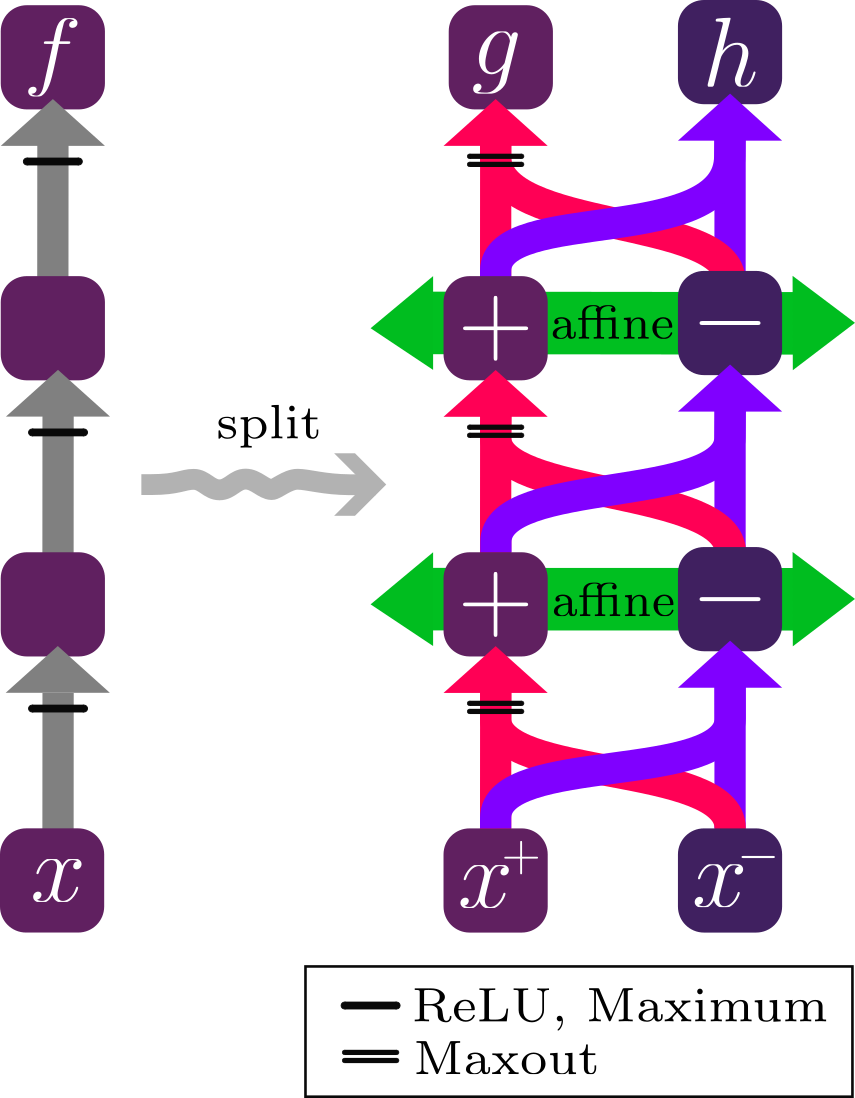
\includegraphics[width=0.28\textwidth]{figures/decompositions/network_split.png}
	\caption[The network splitting procedure]{The network splitting procedure: a \ac{relu} network $f$ is decomposed into two monotone, convex streams $g$ and $h$ with $f = g - h$ (Section~\ref{sec:dc_splitting_relu}).}
	\label{fig:network_split_overview}
\end{figure}

Consider an $L$-layer feedforward network with weights $\Wl{l}$, biases $b^{(l)}$, and entrywise activation $\varrho \colon \RR \to \RR$ (e.g.\ $\relu$ or softplus):
\begin{equation}
	\actl{0} = x,
	\qquad
	\preactl{l} = \Wl{l} \actl{l-1} + b^{(l)},
	\qquad
	\actl{l} = \varrho_l\bigl(\preactl{l}\bigr),
	\qquad l = 1, \dots, L,
	\label{eq:original_forward_pass}
\end{equation}
where $\varrho_l=\varrho$ for $1\leq l<L$ and $\varrho_L=\mathrm{id}$ gives the ungated affine readout $f(x)=\actl{L}\in\RR$. For multi-class networks, fix one target logit. We use the notation of Section~\ref{sec:nn_notation_pwl}, reserving $g,h$ for the split streams of Section~\ref{sec:dc_splitting_relu}.

A decomposition replaces each activation $\actl{l}_i$ by a non-negative pair propagated through non-negative linear maps and \emph{pairwise activation functions}. We first define this structure, then require its differences to recover the original network.

\begin{definition}[Decomposition]\label{def:decomposition}
A \emph{decomposition} of the $L$-layer network~\eqref{eq:original_forward_pass} propagates non-negative activation pairs $\bigl(\act{l}{+}_i, \act{l}{-}_i\bigr) \in \RR^2_{\ge 0}$ from input to output using only
\begin{enumerate}
	\item \textbf{non-negative linear maps}---matrices with non-negative entries together with non-negative bias vectors---and
	\item \textbf{pairwise activation functions} $\phi \colon \RR^2_{\ge 0} \to \RR^2_{\ge 0}$, $(z^+, z^-) \mapsto (a^+, a^-) = \phi(z^+, z^-)$, applied at every hidden neuron; the final affine readout uses the identity on the pair.
\end{enumerate}
Activations are indexed by $l \in \{0,\dots,L\}$, affine parameters by $l \in \{1,\dots,L\}$. The layer-$0$ pair is any non-negative split of the input,
\begin{equation}
	\bigl(\act{0}{+}_k, \act{0}{-}_k\bigr) \coloneqq \bigl(x_k^+, x_k^-\bigr),
	\qquad
	x_k^+ - x_k^- = x_k,
	\qquad
	x_k^+, x_k^- \ge 0,
	\label{eq:input_split_convention}
\end{equation}
and each affine layer $l$ maps the preceding activation pair to a non-negative pre-activation pair $\bigl(\preact{l}{+}_i, \preact{l}{-}_i\bigr)$. The pairwise activation applies for $l<L$; at $l=L$, $\act{L}{\pm}=\preact{L}{\pm}$. We call $\bigl(\act{l}{+}_i,\act{l}{-}_i\bigr)$ the \emph{decomposed activation} and $\bigl(\preact{l}{+}_i,\preact{l}{-}_i\bigr)$ the \emph{decomposed pre-activation}.
\end{definition}

\paragraph{Canonical non-negative linear map.}
We use the entrywise positive/negative split of the original weights and biases,
\begin{equation}
	\Wsig{l}{+} \coloneqq \posneg{\Wl{l}}{+},
	\qquad
	\Wsig{l}{-} \coloneqq \posneg{\Wl{l}}{-},
	\qquad
	b^{(l,+)} \coloneqq \posneg{b^{(l)}}{+},
	\qquad
	b^{(l,-)} \coloneqq \posneg{b^{(l)}}{-},
	\label{eq:canonical_weight_split}
\end{equation}
where $\posneg{\cdot}{\pm}$ are the entrywise positive and negative parts, so $\Wl{l} = \Wsig{l}{+} - \Wsig{l}{-}$ with $\Wsig{l}{\pm} \ge 0$. The resulting pre-activation pair at neuron $i$ is
\begin{align}
	\preact{l}{+}_i &\coloneqq b_i^{(l,+)} + \sum_j \Wsig{l}{+}_{ij}\, \act{l-1}{+}_j + \sum_j \Wsig{l}{-}_{ij}\, \act{l-1}{-}_j,
	\label{eq:split_pos}\\
	\preact{l}{-}_i &\coloneqq b_i^{(l,-)} + \sum_j \Wsig{l}{+}_{ij}\, \act{l-1}{-}_j + \sum_j \Wsig{l}{-}_{ij}\, \act{l-1}{+}_j.
	\label{eq:split_neg}
\end{align}
Positive weights preserve streams; negative weights swap them, turning excitatory contributions into inhibitory ones and vice versa. The following definition connects the structure of Definition~\ref{def:decomposition} to the original network.

\begin{definition}[Valid decomposition]\label{def:valid_decomposition}
A decomposition (Definition~\ref{def:decomposition}) is \emph{valid} for the network~\eqref{eq:original_forward_pass} with activation function $\varrho$ if the propagated activation pairs satisfy
\begin{equation}
	\act{l}{+}_i - \act{l}{-}_i = \varrho_l\bigl(\preactl{l}_i\bigr) = \actl{l}_i
	\label{eq:validity_condition}
\end{equation}
for every layer $l \in \{0, \dots, L\}$ and every neuron $i$, where at $l = 0$ condition~\eqref{eq:validity_condition} is read as $\act{0}{+}_k - \act{0}{-}_k = x_k$.
\end{definition}

Validity propagates through the canonical linear map, recovering the network output at the final layer.

\begin{proposition}[Validity recovers the network, \LeanResult{prop:validity_recovery}]\label{prop:validity_recovery}
Let a decomposition use the canonical non-negative linear map \eqref{eq:split_pos}--\eqref{eq:split_neg}. If the validity condition~\eqref{eq:validity_condition} holds at layer $l-1$, then the decomposed pre-activations at layer $l$ satisfy
\begin{equation}
	\preact{l}{+}_i - \preact{l}{-}_i = \preactl{l}_i
	\qquad \text{for every neuron } i.
	\label{eq:preactivation_difference}
\end{equation}
Consequently, every valid decomposition recovers the original network output as the difference of the final decomposed activations,
\begin{equation}
	f(x) = \act{L}{+} - \act{L}{-}.
	\label{eq:output_recovery}
\end{equation}\end{proposition}

\begin{proof}
Subtracting~\eqref{eq:split_neg} from~\eqref{eq:split_pos} and regrouping by predecessor $j$,
\begin{equation*}
	\preact{l}{+}_i - \preact{l}{-}_i
	= b_i^{(l,+)} - b_i^{(l,-)} + \sum_j \bigl( \Wsig{l}{+}_{ij} - \Wsig{l}{-}_{ij} \bigr) \bigl( \act{l-1}{+}_j - \act{l-1}{-}_j \bigr)
	= b_i^{(l)} + \sum_j \Wl{l}_{ij}\, \actl{l-1}_j
	= \preactl{l}_i,
\end{equation*}
The second equality uses $\Wl{l} = \Wsig{l}{+} - \Wsig{l}{-}$, $b^{(l)} = b^{(l,+)} - b^{(l,-)}$, and validity at layer $l-1$, proving~\eqref{eq:preactivation_difference}. At layer $L$, validity gives $\act{L}{+} - \act{L}{-} = \varrho_L\bigl(\preactl{L}\bigr) = \preactl{L} = f(x)$, proving~\eqref{eq:output_recovery}.
\end{proof}

By Proposition~\ref{prop:validity_recovery}, pre-activation differences recover the original pre-activations. A valid pairwise activation must therefore recover $\varrho(z^+-z^-)$ and preserve non-negativity on the input quadrant. Section~\ref{sec:dc_decompositions} gives conditions for convex, coordinatewise non-decreasing streams, constructs pairs from absolute curvature, and derives ReLU and smooth-activation formulas. Mixing (Section~\ref{sec:mixing_decomposition}), stopping (Section~\ref{sec:stopping_decomposition}), and regularized decompositions (Section~\ref{sec:regularized_decompositions}) preserve the same difference with other structural properties.

\section{Convex and Monotone DC Decompositions}\label{sec:dc_decompositions}

The required activation-level object is a pair of functions $F_+,F_-\colon\RR^2\to\RR$ satisfying
\begin{equation}
    \begin{gathered}
    \varrho(x-y)=F_+(x,y)-F_-(x,y),\\
    F_+,F_-\text{ convex and coordinatewise non-decreasing}.
    \end{gathered}
    \label{eq:general_dc_pair}
\end{equation}
Convexity alone is insufficient for recursive composition: a convex function of convex inputs need not be convex unless the outer function is non-decreasing in those inputs. Conversely, coordinatewise monotonicity does not mean that a function has non-negative values everywhere. We require the pair to be non-negative only on $\RR^2_{\ge0}$, the domain visited by the split network. The global domain $\RR^2$ in~\eqref{eq:general_dc_pair} makes the analytic requirements precise and permits signed inputs to the stream functions.

\subsection{The profile criterion and network composition}

Adding a common affine correction lifts a scalar DC decomposition $\varrho=p-q$ to such a pair. Here $L$ is a slope bound, independent of network depth. The criterion also covers ReLU's kink.

\begin{proposition}[Criterion for a convex, monotone pair, \LeanResult{prop:dc_profile_lift}]\label{prop:dc_profile_lift}
Let $L\ge0$ and $C\colon\RR\to\RR$, and define
\begin{equation}
    T_{C,L}(x,y)\coloneqq C(x-y)+Ly.
    \label{eq:dc_profile_lift}
\end{equation}
Then $T_{C,L}$ is convex on $\RR^2$ if and only if $C$ is convex. It is coordinatewise non-decreasing on $\RR^2$ if and only if
\begin{equation}
    0\le C(v)-C(u)\le L(v-u)\qquad(u\le v).
    \label{eq:dc_profile_increments}
\end{equation}
If $C$ is differentiable, condition~\eqref{eq:dc_profile_increments} is equivalent to $0\le C'\le L$. Consequently, given $p-q=\varrho$, the pair
\begin{equation}
    F_+(x,y)=p(x-y)+Ly,
    \qquad F_-(x,y)=q(x-y)+Ly
    \label{eq:asymmetric_dc_pair}
\end{equation}
is convex and coordinatewise non-decreasing exactly when both profiles are convex and satisfy~\eqref{eq:dc_profile_increments}. Under these conditions it maps $\RR^2_{\ge0}$ to itself exactly when $p(0),q(0)\ge0$.
\end{proposition}

\begin{proof}
Affine precomposition and affine addition preserve convexity; restriction to $y=0$ gives the converse. Increasing $x$ gives the lower bound in~\eqref{eq:dc_profile_increments}; increasing $y$ by $v-u$ changes the argument from $v$ to $u$, giving the upper bound. These inequalities also imply coordinatewise monotonicity. Difference quotients and the mean value theorem give the derivative criterion. The common $Ly$ cancels in $F_+-F_-$. On the non-negative quadrant, monotonicity gives $F_\pm(x,y)\ge F_\pm(0,0)$; evaluation at the origin proves necessity.
\end{proof}

\begin{theoremenv}[Network DC decomposition from activation pairs, \LeanResult{thm:general_dc_network}]\label{thm:general_dc_network}
Consider the network~\eqref{eq:original_forward_pass} with hidden activation $\varrho$. Choose a pair $F_+,F_-$ satisfying~\eqref{eq:general_dc_pair} on all of $\RR^2$ and $F_\pm(0,0)\ge0$. Use this pair entrywise after the canonical affine split~\eqref{eq:split_pos}--\eqref{eq:split_neg}, and use the identity pair at the final affine readout. Then every decomposed activation, and each of the two output streams $G,H$, is convex and coordinatewise non-decreasing as a function of the independent doubled input coordinates $(x^+,x^-)$. Moreover,
\begin{equation}
    G(x^+,x^-)-H(x^+,x^-)=f(x^+-x^-),
    \label{eq:general_network_dc_recovery}
\end{equation}
and both streams are non-negative when $x^+,x^-\ge0$. These conclusions also hold for every tail network starting at an intermediate layer.

If each component of an input split $x\mapsto(x^+(x),x^-(x))$ is convex, then $x\mapsto G(x^+(x),x^-(x))$ and $x\mapsto H(x^+(x),x^-(x))$ are convex. In particular, the usual split $x^\pm=\posneg{x}{\pm}$ gives a DC representation on the original input space.
\end{theoremenv}

\begin{proof}
The initial doubled coordinates are affine and non-decreasing. Non-negative affine combinations preserve convexity and coordinatewise monotonicity, as does composition with each convex, coordinatewise non-decreasing pair component. The final affine layer retains both properties. Induction proves the structural assertions for the network and every tail.

Subtracting each affine pair recovers the original affine map (Proposition~\ref{prop:validity_recovery}); each hidden pair gives $F_+(z^+,z^-)-F_-(z^+,z^-)=\varrho(z^+-z^-)$. The final identity pair gives the ungated pre-activation difference. Induction proves~\eqref{eq:general_network_dc_recovery}, including negative logits. Origin normalization and monotonicity preserve non-negativity at hidden layers, and canonical affine maps preserve it throughout. Composing a convex non-decreasing function with convex components proves the convex input-split assertion \parencite{Amos2017}.
\end{proof}

Monotonicity refers to independent pair coordinates. Under $x^\pm=\posneg{x}{\pm}$, convexity survives, while monotonicity in $x$ generally fails: $x^- =\max\{-x,0\}$ decreases with $x$. The theorem therefore gives monotone networks on doubled space and a DC representation on the original input space.

\subsection{Construction from absolute second derivatives}\label{sec:dc_splitting_smooth}

Finite positive and negative curvature gives bounded profile slopes. We construct them from $|f''|$, with $f$ now denoting a scalar activation.

\begin{theoremenv}[Absolute-curvature construction, \LeanResult{thm:absolute_curvature_split}]\label{thm:absolute_curvature_split}
Let $f\colon\RR\to\RR$ be differentiable, let $f'$ be locally absolutely continuous, and assume $f''\in L^1(\RR)$. Set
\begin{equation}
\begin{gathered}
    s_-\coloneqq\lim_{t\to-\infty}f'(t),\qquad
    V(t)\coloneqq\int_{-\infty}^{t}|f''(u)|\,\diff u,\\
    D(z)\coloneqq |f(0)|+|s_-|z+\int_0^z V(t)\,\diff t,\\
    p\coloneqq\frac{D+f}{2},\qquad q\coloneqq\frac{D-f}{2}.
\end{gathered}
    \label{eq:absolute_curvature_primitive}
\end{equation}
The limits $s_-$ and $s_+\coloneqq\lim_{t\to+\infty}f'(t)$ exist. With
\begin{equation}
    L\coloneqq\frac{\|f''\|_{L^1(\RR)}+|s_-|+|s_+|}{2},
    \label{eq:absolute_curvature_coefficient}
\end{equation}
the profiles $p,q$ are convex, satisfy $p-q=f$ and $0\le p',q'\le L$, and have $p(0)=\max\{f(0),0\}$, $q(0)=\max\{-f(0),0\}$. Therefore~\eqref{eq:asymmetric_dc_pair} is a convex, coordinatewise non-decreasing pair on $\RR^2$, is non-negative on $\RR^2_{\ge0}$, and recovers $f(x-y)$ exactly.
\end{theoremenv}

\begin{proof}
Local absolute continuity gives
$|f'(v)-f'(u)|\le\int_u^v|f''(t)|\,\diff t$ for $u\le v$.
Integrability makes $f'$ Cauchy at both ends of the real line, so its finite limits exist. Write
\begin{equation}
    P=\frac{|f''|+f''}{2},\qquad N=\frac{|f''|-f''}{2}.
    \label{eq:curvature_jordan_parts}
\end{equation}
Differentiating~\eqref{eq:absolute_curvature_primitive} yields
\begin{equation}
    p'(z)=\max\{s_-,0\}+\int_{-\infty}^z P(u)\,\diff u,
    \qquad
    q'(z)=\max\{-s_-,0\}+\int_{-\infty}^z N(u)\,\diff u.
    \label{eq:canonical_profile_slopes}
\end{equation}
Both derivatives are non-negative, non-decreasing, and bounded, and $p''=P$, $q''=N$ almost everywhere. Their upper limits are
$A=\max\{s_-,0\}+\int_{\RR}P$ and
$B=\max\{-s_-,0\}+\int_{\RR}N$.
Since $A+B=|s_-|+\|f''\|_1$ and $A-B=s_+$, their maximum is precisely~\eqref{eq:absolute_curvature_coefficient}. The difference and origin values follow directly from the definition. Proposition~\ref{prop:dc_profile_lift} now proves all pair properties.
\end{proof}

The functions $P$ and $N$ are the positive and negative parts of curvature. They are minimal: any twice weakly differentiable convex profiles $\widetilde p,\widetilde q$ with $\widetilde p-\widetilde q=f$ satisfy $\widetilde p''\ge P$ and $\widetilde q''\ge N$ almost everywhere. Within the affine lift~\eqref{eq:asymmetric_dc_pair}, the coefficient in~\eqref{eq:absolute_curvature_coefficient} is also the least possible common slope bound for globally convex non-decreasing profiles. Indeed, their non-negative limiting slopes at $-\infty$ differ by $s_-$, so they are at least $\max\{s_-,0\}$ and $\max\{-s_-,0\}$; their curvature measures dominate $P\,\diff z$ and $N\,\diff z$. Both upper slope bounds are therefore at least $A$ and $B$ from the proof. This is a minimality statement for this profile-and-affine-lift construction, not for arbitrary bivariate decompositions or for the sizes of the resulting network streams.

\begin{remark}[Why the global domain matters]\label{rem:global_curvature_necessity}
Under the regularity assumptions on $f'$ above, integrability of $f''$ is also necessary for the existence of \emph{finite-valued} convex, coordinatewise non-decreasing $F_+,F_-$ on all of $\RR^2$ with difference $f(x-y)$. To see this, restrict each component to $(t,0)$ for $t\le0$. The resulting convex non-decreasing function has slopes bounded between $0$ and a finite one-sided slope at the origin, hence finite curvature mass on the negative half-line. Next restrict each component to $(0,-t)$ for $t\ge0$. These restrictions are convex and non-increasing, so their slopes lie between a finite slope at the origin and $0$, giving finite curvature mass on the positive half-line. In both restrictions the difference is $f(t)$; the total variation of its curvature is bounded by the sum of the two positive curvature measures. Thus $\int_{\RR}|f''|<\infty$. This necessity argument concerns the global domain and does not apply if the pair is defined only on the non-negative quadrant. For example,
\begin{equation*}
    (x-y)^2=\bigl(2x^2+2y^2\bigr)-(x+y)^2
\end{equation*}
is a difference of two convex, coordinatewise non-decreasing functions on that quadrant, although the curvature of $f(z)=z^2$ is not integrable on $\RR$.
\end{remark}

\begin{corollary}[Exact splitting on a bounded activation interval]\label{cor:local_curvature_split}
Let $a<b$ and let $f\in C^1([a,b])$ have absolutely continuous derivative. There exist finite-valued convex, coordinatewise non-decreasing functions $F_+,F_-\colon\RR^2\to\RR$, non-negative on $\RR^2_{\ge0}$, such that $F_+(x,y)-F_-(x,y)=f(x-y)$ whenever $x-y\in[a,b]$.
\end{corollary}

\begin{proof}
Extend $f$ by its tangent affine functions at $a$ and $b$. The extension is continuously differentiable, its derivative is locally absolutely continuous, and its curvature vanishes outside $[a,b]$. Apply Theorem~\ref{thm:absolute_curvature_split} to this extension.
\end{proof}

This local statement applies, for example, to exponentiation on a fixed bounded score interval. It does not assert a global monotone convex split for $e^z$ on all of $\RR$, whose curvature is not integrable.

\subsection{ReLU: the maximum and identity pair}\label{sec:dc_splitting_relu}

For $f(z)=\relu(z)$ choose $p(z)=\relu(z)$, $q(z)=0$, and $L=1$. Both profiles are convex and satisfy~\eqref{eq:dc_profile_increments}, even though $p$ is not differentiable at the origin. The profile lift gives the exact pair
\begin{equation}
    \begin{gathered}
    F_+(a,b)=\relu(a-b)+b=\max\{a,b\},\qquad F_-(a,b)=b,\\
    \relu(a-b)=\max\{a,b\}-b.
    \end{gathered}
    \label{eq:splitting_identity}
\end{equation}
This specializes the general criterion to a positive Maxout component \parencite{Goodfellow2013Maxout} and a negative identity component. Replacing $f''\,\diff z$ by $\delta_0$ in the absolute-curvature construction gives the same pair (Remark~\ref{rem:bv_extension}). This classical ReLU-network DC split \parencite{Zhang2018,Siahkamari2020_DCRegression,Awasthi2023DCNN,hiddenMono} underlies our stabilized passes, CNN extension, and saliency methods.

The hidden-layer update is therefore
\begin{equation}
    \act{l}{+}=\max\{\preact{l}{+},\preact{l}{-}\},
    \qquad \act{l}{-}=\preact{l}{-},\qquad 1\le l<L,
    \label{eq:dc_split_activations}
\end{equation}
with $\act{L}{\pm}=\preact{L}{\pm}$ at the final affine readout. Theorem~\ref{thm:general_dc_network} gives validity and convexity. Section~\ref{sec:mixing_decomposition} identifies this as the mixing family's $\eta=1$ endpoint.

\begin{figure}[htbp]
	\centering
	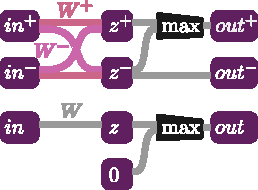
\includegraphics[width=.35\linewidth]{figures/decompositions/split_streams.pdf}
	\caption[Monotone, convex split streams and a standard ReLU layer]{Monotone, convex split streams (top) and a standard \ac{relu} layer (bottom). Negative weights swap positive and negative input streams into opposite pre-activation streams; positive weights preserve them.}
	\label{fig:splitstreams}
\end{figure}

\paragraph{The stream functions $g$ and $h$.}
The \ac{dc} \emph{split pair} consists of two monotone \emph{split streams}, non-negative on the input quadrant (Figure~\ref{fig:splitstreams}). Like the tail network $f^{(l)} \colon \RR^{d^{(l)}} \to \RR$ on layers $l+1, \dots, L$, define the restricted streams
\begin{equation}
	g^{(l)} \colon \RR^{d^{(l)}} \times \RR^{d^{(l)}} \to \RR,
	\qquad
	h^{(l)} \colon \RR^{d^{(l)}} \times \RR^{d^{(l)}} \to \RR,
	\label{eq:stream_functions}
\end{equation}
mapping an activation pair at layer $l$ to the $+$ and $-$ components of the decomposed output; we abbreviate $g \coloneqq g^{(0)}$, $h \coloneqq h^{(0)}$. On the output layer $g^{(L)}(x^+, x^-) = x^+$, $h^{(L)}(x^+, x^-) = x^-$, and for $0 \le l < L$,
\begin{equation}
	g^{(l)}(x^+, x^-) = g^{(l+1)}\bigl(\act{l+1}{+}, \act{l+1}{-}\bigr),
	\qquad
	h^{(l)}(x^+, x^-) = h^{(l+1)}\bigl(\act{l+1}{+}, \act{l+1}{-}\bigr),
	\label{eq:stream_recursion}
\end{equation}
where \eqref{eq:split_pos}--\eqref{eq:split_neg} and \eqref{eq:dc_split_activations} compute $\bigl(\act{l+1}{+}, \act{l+1}{-}\bigr)$ from $(x^+,x^-)$. These full tail functions, rather than individual layer activations, define $f=g-h$ and underpin Chapter~\ref{ch:saliency}. The \ac{mlp} split pass starts from $\bigl(\act{0}{+},\act{0}{-}\bigr)=(x^+,x^-)$, then applies the affine pair \eqref{eq:split_pos}--\eqref{eq:split_neg} and the maximum/identity update~\eqref{eq:dc_split_activations} for $l=1,\dots,L-1$. The final layer uses only the affine pair, allowing negative reconstructed logits.

Non-negative affine maps followed by Maxout gates and projections form monotone networks with convex, monotone activations. The composition principles of Section~\ref{sec:convex_monotone_foundations} \parencite{Amos2017} give:

\begin{proposition}[Monotonicity and convexity of the split streams, \LeanResult{prop:stream_properties}]\label{prop:stream_properties}
For every $0 \le l \le L$, the stream functions $g^{(l)}$ and $h^{(l)}$ of~\eqref{eq:stream_functions} are convex and non-decreasing in each coordinate of the pair $(x^+, x^-) \in \RR^{d^{(l)}} \times \RR^{d^{(l)}}$.\end{proposition}

\begin{proof}
Apply Theorem~\ref{thm:general_dc_network} to each tail network using the pair $(\max\{a,b\},b)$ from~\eqref{eq:splitting_identity}. The final pair is the identity, so the same argument includes the ungated affine head.
\end{proof}

The correctness statement asserts that the difference of the two split-stream outputs equals the original tail network evaluated at the difference of their inputs---at \emph{every} layer, not only at the input.

\begin{theoremenv}[Correctness of the split forward pass, \LeanResult{thm:split_correct}]\label{thm:split_correct}
For every $0 \le l \le L$ and all $x^+, x^- \in \RR^{d^{(l)}}_{\ge 0}$,
\begin{equation}
	f^{(l)}\bigl( x^+ - x^- \bigr)
	= \bigl( g^{(l)} - h^{(l)} \bigr)(x^+, x^-).
	\label{eq:split_correctness}
\end{equation}\end{theoremenv}

\begin{proof}
Apply Theorem~\ref{thm:general_dc_network} to each tail. Hidden-pair subtraction gives $\relu(z^+-z^-)$ by~\eqref{eq:splitting_identity}, and final-pair subtraction gives $z^+-z^-$ since $\varrho_L=\mathrm{id}$. The identity tail at $l=L$ and recursion~\eqref{eq:stream_recursion} give~\eqref{eq:split_correctness} at every layer.
\end{proof}

\begin{remark}[Preservation of sub-threshold signals]\label{rem:subthreshold}
At an inactive neuron, $\preactl{l}_i\le0$, ReLU outputs $\actl{l}_i=0$, discarding the losing pre-activation's magnitude. Downstream computation cannot distinguish degrees of suppression. The split pair $\bigl(\act{l}{+}_i,\act{l}{-}_i\bigr)=\bigl(\preact{l}{-}_i,\preact{l}{-}_i\bigr)$ has the required zero difference while retaining the cancelled mass $\preact{l}{-}_i$ in both components. These sub-threshold contributions give the streams more information than the original activations, which Chapter~\ref{ch:saliency} exploits. Retaining them also causes the numerical growth of Section~\ref{sec:stabilization_dc}: without subtractive cancellation, the streams accumulate absolute mass $\preact{l}{+}_i+\preact{l}{-}_i$ instead of the signed residual.
\end{remark}

\begin{remark}[Flexibility of the input split]\label{rem:input_split_flexibility}
Theorem~\ref{thm:split_correct} allows \emph{any} non-negative representation $x=x^+-x^-$, including $x^\pm=\posneg{x}{\pm}$ and $x^\pm=\posneg{x}{\pm}+c$ with $c\ge0$. Numerical stabilization and Chapter~\ref{ch:saliency}'s attribution baselines exploit this freedom. The half--half split $x^\pm=\pm x/2$ (Section~\ref{sec:stabilization_dc}) instead has signed components: it serves only as a backward chain-rule device along the unified input direction.
\end{remark}

\subsection{Closed formulas for smooth activations}\label{sec:closed_form_dc_activations}

The following activations admit explicit absolute-curvature profiles. Smooth curvature majorants yield shorter formulas, so we give both and distinguish exact recovery from minimal curvature. Write $\sigma(z)=(1+e^{-z})^{-1}$, let $\varphi,\Phi$ be the standard Gaussian density and distribution function, and set
\begin{equation*}
    s_\beta(z)\coloneqq\frac{1}{\beta}\log(1+e^{\beta z}),\qquad \beta>0.
\end{equation*}

\begin{corollary}[Explicit convex, monotone activation pairs, \LeanResult{cor:closed_form_dc_activations}]\label{cor:closed_form_dc_activations}
For $f(z)=z\Phi(z)$ (GELU), $f(z)=z\sigma(\beta z)$ (Swish), $f=\sigma$ (sigmoid), and $f=s_{1/\theta}$ (softplus), choose the corresponding row of Table~\ref{tab:closed_form_dc_profiles}. Then the functions $F_+(x,y)=p(x-y)+Ly$ and $F_-(x,y)=q(x-y)+Ly$ are convex and coordinatewise non-decreasing on $\RR^2$, map $\RR^2_{\ge0}$ to itself, and satisfy $F_+-F_-=f(x-y)$.
\end{corollary}

\begin{table}[htbp]
\TableContent{
\centering
\small
\setlength{\tabcolsep}{5pt}
\begin{tabularx}{\linewidth}{@{}l>{\raggedright\arraybackslash}X>{\raggedright\arraybackslash}Xc@{}}
\toprule
Activation & $p(z)$ & $q(z)$ & $L$ \\
\midrule
GELU & $2z\Phi(z)+2\varphi(z)$ & $z\Phi(z)+2\varphi(z)$ & $2$ \\[3pt]
Swish & $2s_\beta(z)$ & $2s_\beta(z)-z\sigma(\beta z)$ & $2$ \\[3pt]
Sigmoid & $\tfrac12(s_1(z)+\sigma(z))$ & $\tfrac12(s_1(z)-\sigma(z))$ & $\tfrac12$ \\[3pt]
Softplus & $s_{1/\theta}(z)$ & $0$ & $1$ \\
\bottomrule
\end{tabularx}
}%
\caption[Closed scalar profiles for smooth activations]{Closed profiles for~\eqref{eq:asymmetric_dc_pair}, $\beta,\theta>0$. GELU, Swish, and sigmoid trade additional curvature for shorter smooth formulas. GELU denotes the exact Gaussian activation, excluding its tanh approximation; SiLU is Swish with $\beta=1$.}
\label{tab:closed_form_dc_profiles}
\end{table}

\begin{proof}
In every row $p-q=f$. For GELU \parencite{Hendrycks2016}, direct differentiation gives
\begin{equation*}
    p'=2\Phi,\quad p''=2\varphi,\qquad
    q'=\Phi-z\varphi,\quad q''=z^2\varphi.
\end{equation*}
Hence both profiles are convex; $p'$ increases from $0$ to $2$ and $q'$ from $0$ to $1$. For Swish \parencite{Ramachandran2017_swish}, writing $u=\beta z$ gives
\begin{equation*}
    p'=2\sigma(u),\quad p''=2\beta\sigma'(u),\qquad
    q'=\sigma(u)-u\sigma'(u),\quad
    q''=\beta u\bigl(2\sigma(u)-1\bigr)\sigma'(u)\ge0.
\end{equation*}
The last inequality uses that $u$ and $2\sigma(u)-1$ have the same sign. The slopes again have limits $0,2$ for $p'$ and $0,1$ for $q'$, so they lie in $[0,2]$. For the sigmoid profiles,
\begin{equation*}
    p'=\tfrac12\sigma(2-\sigma),\quad
    q'=\tfrac12\sigma^2,\qquad
    p''=\sigma'(1-\sigma)\ge0,\quad q''=\sigma'\sigma\ge0,
\end{equation*}
with slopes in $[0,1/2]$. Softplus has $p'=\sigma(z/\theta)\in[0,1]$ and $p''=\sigma'(z/\theta)/\theta\ge0$, while $q=0$. All profile values at zero are non-negative (for sigmoid, $s_1(0)=\log2>1/2$). Proposition~\ref{prop:dc_profile_lift} proves the claim.
\end{proof}

These formulas require no numerical integration or auxiliary root solve. For example, the softplus row simplifies directly to
\begin{equation}
    F_+(x,y)=\theta\log\bigl(e^{x/\theta}+e^{y/\theta}\bigr),
    \qquad F_-(x,y)=y,
    \label{eq:softplus_dc_closed}
\end{equation}
whose limit as $\theta\downarrow0$ is exactly $(\max\{x,y\},y)$. The sigmoid row gives
\begin{equation}
    F_\pm(x,y)=\frac{\log(e^x+e^y)\pm\sigma(x-y)}{2}.
    \label{eq:sigmoid_dc_closed}
\end{equation}
Writing $d=x-y$, the GELU and Swish pairs are explicitly
\begin{equation}
\begin{aligned}
    F_+^{\mathrm{GELU}}(x,y)&=2\bigl(d\Phi(d)+\varphi(d)+y\bigr),\\
    F_-^{\mathrm{GELU}}(x,y)&=d\Phi(d)+2\varphi(d)+2y,
\end{aligned}
    \label{eq:gelu_dc_closed}
\end{equation}
and
\begin{equation}
\begin{aligned}
    F_+^{\mathrm{Swish}}(x,y)&=\frac{2}{\beta}\log\bigl(e^{\beta x}+e^{\beta y}\bigr),\\
    F_-^{\mathrm{Swish}}(x,y)&=F_+^{\mathrm{Swish}}(x,y)-d\sigma(\beta d).
\end{aligned}
    \label{eq:swish_dc_closed}
\end{equation}
Stable implementations of the exponential formulas should evaluate log-sum-exp through its usual shifted form.

\paragraph{Closed forms for the canonical absolute-curvature split.}
The smaller coefficients in Theorem~\ref{thm:absolute_curvature_split} can also be attained explicitly. For sigmoid,
\begin{equation}
    p(z)=\begin{cases}
        \sigma(z),&z\le0,\\
        \tfrac12+\tfrac14z,&z\ge0,
    \end{cases}
    \qquad q(z)=p(z)-\sigma(z),\qquad L=\tfrac14.
    \label{eq:sigmoid_canonical_dc}
\end{equation}
For both GELU and Swish, let $a>0$ be the positive zero of $f''$, and define $m=f'(a)-1$, $c=af'(a)-f(a)$ and $L=1+2m$. Then
\begin{equation}
    p(z)=\begin{cases}
        -c,&z\le-a,\\
        f(z)+mz,&-a\le z\le a,\\
        Lz-c,&z\ge a,
    \end{cases}
    \qquad q(z)=p(z)-f(z).
    \label{eq:gelu_swish_canonical_dc}
\end{equation}
The constants are
\begin{equation}
\begin{aligned}
    \text{GELU:}\quad &a=\sqrt2,\quad
    m=\Phi(\sqrt2)+\sqrt2\varphi(\sqrt2)-1,\quad c=2\varphi(\sqrt2),\\
    \text{Swish:}\quad &a=r/\beta,\quad m=(r-2)/4,\quad
    c=(r^2-4)/(4\beta),\quad L=r/2,
\end{aligned}
    \label{eq:canonical_activation_constants}
\end{equation}
where $r$ uniquely solves $r\tanh(r/2)=2$ on $r>0$ ($r\approx2.39936$): the left-hand side increases strictly from $0$ to infinity. Fixing $r$ gives a pointwise Swish formula without quadrature. Softplus already uses the canonical profiles in Table~\ref{tab:closed_form_dc_profiles}.

For~\eqref{eq:gelu_swish_canonical_dc}, both activations satisfy $f(-z)=f(z)-z$, $f'(-\infty)=0$, $f'(+\infty)=1$, and have positive curvature precisely on $(-a,a)$. Piecewise differentiation gives $p''=\max\{f'',0\}$, $q''=\max\{-f'',0\}$, with matching values and first derivatives at $\pm a$. Since $p(0)=q(0)=0$, these are Theorem~\ref{thm:absolute_curvature_split}'s normalized profiles. Sigmoid's curvature changes sign at zero, giving~\eqref{eq:sigmoid_canonical_dc} analogously. Canonical GELU and Swish profiles can be negative on the negative half-line; origin normalization and coordinatewise monotonicity ensure their lifted pairs are non-negative on the required quadrant.

\begin{corollary}[Modern activation functions, \LeanResult{cor:modern_activations}]\label{cor:modern_activations}
Theorems~\ref{thm:absolute_curvature_split} and~\ref{thm:smooth_dc_split} apply to the following activation functions, where $\varphi$ and $\Phi$ denote the standard Gaussian density and distribution function and $\sigma(x) = (1+e^{-x})^{-1}$ the logistic sigmoid:
\begin{enumerate}
	\item \emph{GELU}, $f(x) = x\,\Phi(x)$, with $f''(x) = (2 - x^2)\,\varphi(x)$; the curvature is positive on $(-\sqrt{2}, \sqrt{2})$ and negative outside.
	\item \emph{Swish/SiLU}, $f(x) = x\,\sigma(\beta x)$ with $\beta > 0$, with $f''(x) = \beta\,\sigma'(\beta x)\bigl( 2 + \beta x\,(1 - 2\sigma(\beta x)) \bigr)$; the curvature is positive on a bounded interval around the origin and negative in both tails.
	\item \emph{Mish}, $f(x) = x \tanh\bigl(\log(1 + e^{x})\bigr)$.
	\item \emph{Hyperbolic tangent}, $f(x) = \tanh(x)$, with $f''(x) = -2 \tanh(x)\operatorname{sech}^2(x)$, so $P$ is supported on $(-\infty, 0]$ and $N$ on $[0, \infty)$.
	\item \emph{Logistic sigmoid}, $f = \sigma$, with $f'' = \sigma'\,(1 - 2\sigma)$.
	\item \emph{Softplus at temperature $\theta > 0$}, $f(x) = \theta \log(1 + e^{x/\theta})$, with $f''(x) = \sigma'(x/\theta)/\theta \ge 0$; here $N = 0$, $C_2 = 0$, and the decomposition degenerates to the statement that softplus itself is convex.
\end{enumerate}
In each case $f(0) \ge 0$, and both constructions preserve non-negativity on the input quadrant (Remark~\ref{rem:smooth_valid_decomposition}).\end{corollary}

\begin{proof}
Direct differentiation gives the stated second derivatives. Each $f''$ is continuous and decays at least exponentially as $\abs{x}\to\infty$ (Gaussian for GELU). For Swish and Mish, exponential decay of $\sigma'(\beta x)$ and the derivatives of $\tanh\circ\operatorname{softplus}$ dominates the polynomial factor $x$. Thus $f''\in L^1(\RR)$ and $f'$ is locally absolutely continuous. Both constructions apply, with non-negative $f(0)\in\{0,\tfrac12,\theta\log2\}$.
\end{proof}

\begin{corollary}[Networks with smooth activations, \LeanResult{cor:smooth_dc_networks}]\label{cor:smooth_dc_networks}
Every finite feedforward network with GELU, Swish/SiLU, sigmoid, or softplus hidden activations, arbitrary signed weights and biases, and an affine output admits an exact decomposition into two convex, coordinatewise non-decreasing streams on doubled input space. Either the explicit profiles of Corollary~\ref{cor:closed_form_dc_activations} or the canonical profiles~\eqref{eq:sigmoid_canonical_dc}--\eqref{eq:gelu_swish_canonical_dc} and~\eqref{eq:softplus_dc_closed} may be used at every hidden neuron. With the usual non-negative input split, the streams remain non-negative and their pullbacks are convex functions of the original signed input. The same existence result holds for Mish and tanh by Theorem~\ref{thm:absolute_curvature_split}.
\end{corollary}

\begin{proof}
The activation pairs have the properties required by Theorem~\ref{thm:general_dc_network}, by Corollaries~\ref{cor:closed_form_dc_activations} and~\ref{cor:modern_activations}; apply that theorem with the identity pair at the output.
\end{proof}

The induction also permits different qualifying activations or profiles at each hidden layer. The theorem states the uniform-activation case used by the formal network interface.

\begin{remark}[Scope of the smooth extension]\label{rem:smooth_pointer}
The extension above is an exact structural theorem about the scalar activations and their composition into feedforward networks. It does not establish empirical attribution quality for these smooth networks, nor does it by itself extend the ReLU-specific hard-gate games or numerical stabilization formulas. The experiments later in the thesis evaluate the architectures and methods described in their protocols; the new smooth formulas are not additional experimental results.
\end{remark}

\subsection{Multivariate activations and softmax}\label{sec:multivariate_dc_softmax}

For activations coupling coordinates, convexity means componentwise convexity of each vector-valued pair. This differentiable lift suffices for softmax.

\begin{proposition}[Multivariate profile lift, \LeanResult{prop:multivariate_dc_lift}]\label{prop:multivariate_dc_lift}
Let $C\in C^1(\RR^n)$ and $\ell\in\RR^n_{\ge0}$. Define
\begin{equation}
    T_{C,\ell}(x,y)=C(x-y)+\langle\ell,y\rangle,
    \qquad x,y\in\RR^n.
    \label{eq:multivariate_dc_lift}
\end{equation}
Then $T_{C,\ell}$ is convex on $\RR^{2n}$ if and only if $C$ is convex, and is coordinatewise non-decreasing if and only if
$0\le\partial_j C(z)\le\ell_j$ for all $z$ and $j$.
Consequently, if $C_+-C_-=f$, both profiles are convex, and both satisfy these derivative bounds, the common lift gives a convex, coordinatewise non-decreasing pair with difference $f(x-y)$. If $C_+(0),C_-(0)\ge0$, the lifted pair is non-negative on $\RR^{2n}_{\ge0}$.
\end{proposition}

\begin{proof}
Affine precomposition preserves convexity; restriction to $y=0$ gives the converse. The derivatives $\partial_{x_j}T=\partial_jC$ and $\partial_{y_j}T=\ell_j-\partial_jC$ give the monotonicity criterion. The common affine term cancels, and monotonicity bounds values on the non-negative orthant by their origin values.
\end{proof}

Softmax admits a short pair because the log-sum-exp Hessian dominates its curvature. This uses multivariate curvature comparison, not the scalar integrability theorem.

\begin{theoremenv}[Explicit convex, monotone softmax pair, \LeanResult{thm:softmax_dc_split}]\label{thm:softmax_dc_split}
Let $n\ge1$, and define
\begin{equation*}
    H(z)=\log\!\left(\sum_{j=1}^n e^{z_j}\right),
    \qquad \pi_i(z)=\frac{e^{z_i}}{\sum_{j=1}^n e^{z_j}},
    \qquad c_n=\frac{\log n-1/n}{2}.
\end{equation*}
For each output coordinate $i$, set
\begin{equation}
    F_{i,\pm}(x,y)
    =\frac{H(x-y)\pm\pi_i(x-y)+\sum_{j=1}^n y_j}{2}-c_n.
    \label{eq:softmax_dc_pair}
\end{equation}
Both components are finite, convex, and coordinatewise non-decreasing on all of $\RR^{2n}$. They are non-negative on $\RR^{2n}_{\ge0}$ and satisfy
$F_{i,+}(x,y)-F_{i,-}(x,y)=\pi_i(x-y)$.
\end{theoremenv}

\begin{proof}
Fix $z$ and a direction $v\in\RR^n$, and abbreviate
$\mu=\sum_j\pi_j(z)v_j$ and
$V=\sum_j\pi_j(z)(v_j-\mu)^2$.
Differentiation along $z+tv$ gives
\begin{equation}
\begin{aligned}
    D^2H(z)[v,v]&=V,\\
    D^2\pi_i(z)[v,v]
    &=\sum_j\pi_j(z)\bigl(\1[j=i]-\pi_i(z)\bigr)(v_j-\mu)^2.
\end{aligned}
    \label{eq:softmax_curvature_domination}
\end{equation}
Since $|\1[j=i]-\pi_i|\le1$, it follows that
$|D^2\pi_i(z)[v,v]|\le V$. Thus $H+\pi_i$ and $H-\pi_i$ have positive semidefinite Hessians and are convex. For the profiles $C_{i,\pm}=(H\pm\pi_i)/2-c_n$, their partial derivatives are
\begin{equation}
\begin{array}{c|cc}
 & \partial_j C_{i,+} & \partial_j C_{i,-}\\ \hline
 j=i & \pi_i-\pi_i^2/2 & \pi_i^2/2\\
 j\ne i & \pi_j(1-\pi_i)/2 & \pi_j(1+\pi_i)/2.
\end{array}
    \label{eq:softmax_profile_gradients}
\end{equation}
Every entry lies in $[0,1/2]$; for the last entry, use $\pi_j\le1-\pi_i$. Proposition~\ref{prop:multivariate_dc_lift} with $\ell_j=1/2$ gives global convexity and monotonicity. At the origin, $F_{i,+}(0,0)=1/n$ and $F_{i,-}(0,0)=0$, proving non-negativity on the orthant. Subtraction gives exact recovery.
\end{proof}

For fixed masked softmax, apply the theorem to each row's nonempty allowed set and assign masked outputs $(0,0)$. Fully masked rows require a separate convention and lie outside this theorem. Fixed positive temperatures and fixed additive score biases enter the preceding affine map. Section~\ref{sec:transformer_dc} combines this pair with convex product and normalization pairs to split the full Transformer.

\subsection{The symmetric-tilt variant and curvature minimality}\label{sec:symmetric_curvature_variant}

A symmetric alternative uses the same curvature split with common tilt $M(a+b)$. Its fixed-profile minimality is independent of~\eqref{eq:asymmetric_dc_pair}. Both constructions recover the same difference, generally with different streams; only the asymmetric normalization above gives the literal ReLU pair $(\max\{a,b\},b)$.

\begin{theoremenv}[DC--monotone splitting under integrable curvature, \LeanResult{thm:smooth_dc_split}]\label{thm:smooth_dc_split}
Let $f\colon \RR \to \RR$ be differentiable with locally absolutely continuous derivative $f'$ and $f'' \in L^1(\RR)$. Then the limit $s_- \coloneqq \lim_{u\to-\infty} f'(u)$ exists and $f'$ is bounded. Write $P \coloneqq \max\{f'',0\}$ and $N \coloneqq \max\{-f'',0\}$, so that $f'' = P - N$ with $P, N \ge 0$, and define
\begin{align}
	C_1(x) &\coloneqq f(0) + \int_0^x \Bigl( s_- + \int_{-\infty}^t P(u)\,\diff u \Bigr) \diff t,
	&
	C_2(x) &\coloneqq \int_0^x \int_{-\infty}^t N(u)\,\diff u \,\diff t,
	\label{eq:curvature_antiderivatives}
\end{align}
as well as $M \coloneqq \max\bigl\{ \sup_{x\in\RR} \abs{C_1'(x)},\, \sup_{x\in\RR} \abs{C_2'(x)} \bigr\} < \infty$. Then the functions
\begin{equation}
	g(a,b) \coloneqq C_1(a-b) + M(a+b),
	\qquad
	h(a,b) \coloneqq C_2(a-b) + M(a+b)
	\label{eq:smooth_split_pair}
\end{equation}
are convex on $\RR^2$, non-decreasing in each argument, and satisfy
\begin{equation}
	f(a-b) = g(a,b) - h(a,b) \qquad \text{for all } (a,b) \in \RR^2.
	\label{eq:smooth_splitting_identity}
\end{equation}\end{theoremenv}

\begin{proof}
\emph{Well-definedness.}
For $x \le y$ we have $\abs{f'(y) - f'(x)} \le \int_x^y \abs{f''(u)} \diff u$, which tends to $0$ as $x, y \to -\infty$ because $f'' \in L^1(\RR)$; by the Cauchy criterion the limit $s_-$ exists. Consequently $\abs{f'(x)} \le \abs{s_-} + \norm{f''}_{L^1(\RR)}$ for all $x$, so the boundedness of $f'$ is automatic and need not be assumed. Since $0 \le P, N \le \abs{f''}$, both $P$ and $N$ lie in $L^1(\RR)$, the inner integrals in \eqref{eq:curvature_antiderivatives} are well-defined, non-decreasing in $t$, and bounded by $\norm{P}_{L^1(\RR)}$ and $\norm{N}_{L^1(\RR)}$ respectively. Hence $C_1, C_2$ are well-defined with locally absolutely continuous derivatives
\begin{equation*}
	C_1'(x) = s_- + \int_{-\infty}^{x} P(u) \,\diff u,
	\qquad
	C_2'(x) = \int_{-\infty}^{x} N(u) \,\diff u,
\end{equation*}
and $\abs{C_1'} \le \abs{s_-} + \norm{P}_{L^1(\RR)}$, $\abs{C_2'} \le \norm{N}_{L^1(\RR)}$, so $M < \infty$.

\emph{Exactness.}
For almost every $x$,
\begin{equation*}
	C_1'(x) - C_2'(x) = s_- + \int_{-\infty}^{x} \bigl( P(u) - N(u) \bigr) \diff u = s_- + \int_{-\infty}^{x} f''(u) \,\diff u = f'(x),
\end{equation*}
Integrating from $0$, with $C_1(0)-C_2(0)=f(0)$, gives $C_1-C_2=f$ on $\RR$. The common tilt cancels, proving~\eqref{eq:smooth_splitting_identity} at $x=a-b$.

\emph{Convexity.}
Since $P,N\ge0$, their (shifted) antiderivatives $C_1',C_2'$ are non-decreasing, so $C_1,C_2$ are convex. Linear precomposition by $(a,b)\mapsto a-b$ and addition of $M(a+b)$ preserve convexity, giving convex $g,h$ on $\RR^2$. When $f''$ is continuous, the Hessian of $C_1(a-b)$ has eigenvalues $0$ and $2C_1''(a-b)=2P(a-b)\ge0$.

\emph{Monotonicity.}
By the choice of $M$,
\begin{equation*}
	\frac{\partial g}{\partial a}(a,b) = C_1'(a-b) + M \ge 0,
	\qquad
	\frac{\partial g}{\partial b}(a,b) = -C_1'(a-b) + M \ge 0,
\end{equation*}
and analogously for $h$ with $C_2'$ in place of $C_1'$. Hence $g$ and $h$ are non-decreasing in each argument.
\end{proof}

The curvature split is canonical. For the fixed profiles~\eqref{eq:curvature_antiderivatives}, $M$ minimizes symmetric tilts $\lambda(a+b)$; this does not compare asymmetric corrections or other profile normalizations.

\begin{proposition}[Minimality of the curvature split, \LeanResult{prop:curvature_minimality}]\label{prop:curvature_minimality}
Let $f$ be as in Theorem~\ref{thm:smooth_dc_split} and suppose $f = c_1 - c_2$ for convex functions $c_1, c_2 \colon \RR \to \RR$ whose second distributional derivatives are locally integrable functions. Then $c_1'' \ge P$ and $c_2'' \ge N$ almost everywhere. In particular, $(C_1, C_2)$ is, up to a common affine summand, the unique pair of convex functions with $C_1 - C_2 = f$ of pointwise minimal curvature, and among all tilts of the form $(a,b) \mapsto \lambda(a+b)$, $\lambda \ge 0$, the constant $M$ in Theorem~\ref{thm:smooth_dc_split} is the smallest one rendering both components of \eqref{eq:smooth_split_pair} non-decreasing in each argument.\end{proposition}

\begin{proof}
Convexity gives $c_1''=f''+c_2''\ge f''$ and $c_1''\ge0$, hence $c_1''\ge\max\{f'',0\}=P$ almost everywhere; symmetrically, $c_2''\ge N$. Equality a.e.\ in both bounds makes $c_1-C_1$ and $c_2-C_2$ affine. They coincide because $c_1-c_2=f=C_1-C_2$. Monotonicity in both arguments requires $\lambda\ge\pm C_1'(x)$ for all $x$, equivalently $\lambda\ge\sup_x\abs{C_1'(x)}$, and likewise for $C_2'$. The least admissible $\lambda$ is $M$.
\end{proof}

\begin{remark}[Bounded variation and the piecewise-linear case]\label{rem:bv_extension}
The construction extends to locally absolutely continuous $f$ whose weak derivative has a bounded-variation representative, with finite signed Radon curvature measure $\mu$. Substitute $|\mu|$ for $|f''(u)|\,\diff u$ in Theorem~\ref{thm:absolute_curvature_split}, or Jordan parts $\mu_+,\mu_-$ for $P(u)\,\diff u,N(u)\,\diff u$. The resulting profiles are convex with bounded slopes; criterion~\eqref{eq:dc_profile_increments} handles kinks. ReLU has $\mu=\delta_0$, $s_-=0$, giving $p(z)=\max\{z,0\}$, $q=0$, $L=1$, hence exactly $(\max\{a,b\},b)$ under the asymmetric lift. The symmetric variant gives $(\relu(a-b)+a+b,a+b)$. Leaky ReLU with slope $\alpha$ has curvature $(1-\alpha)\delta_0$; standard ELU with unit negative-branch scale has curvature $e^z\indicator{z<0}\,\diff z$. Both fit this finite-measure construction, unifying piecewise-linear and smooth activations through bounded variation.
\end{remark}

\begin{remark}[Compatibility with valid decompositions]\label{rem:smooth_valid_decomposition}
Both constructions fit Definition~\ref{def:decomposition}. The asymmetric pair has non-negative origin values $F_+(0,0)=\max\{f(0),0\}$, $F_-(0,0)=\max\{-f(0),0\}$; monotonicity gives non-negativity on $\RR^2_{\ge0}$. The symmetric pair~\eqref{eq:smooth_split_pair} has $g(0,0)=f(0)$, $h(0,0)=0$, so this holds whenever $f(0)\ge0$, including Corollary~\ref{cor:modern_activations}. If $f(0)<0$, adding $|f(0)|$ to both components restores non-negativity and preserves their difference. Exactness gives activation-level validity; Theorem~\ref{thm:general_dc_network} gives network recovery, convexity, and monotonicity.
\end{remark}

\section{The Mixing Decomposition family}\label{sec:mixing_decomposition}

ReLU networks compute \ac{cpwl} functions \parencite{Arora2018} admitting \ac{dc} decompositions \parencite{Melzer1986_PLasDC,Kripfganz1987_PWAasDC,hiddenMono}. We extend the ReLU pair to a one-parameter family of pairwise activations interpolating between two arithmetic extremes.

\begin{definition}[Mixing decomposition function, \LeanResult{def:fmix}]\label{def:fmix}
For $\eta \in [0,1]$, the \emph{mixing decomposition function} is
\begin{equation}
	\fmix(z^+, z^-) \coloneqq \bigl(\, \eta \max\{z^+, z^-\} + (1-\eta)\, z^+, \;\; \eta\, z^- + (1-\eta) \min\{z^+, z^-\} \,\bigr).
	\label{eq:fmix_def}
\end{equation}
The \emph{Mixing Decomposition} uses $\fmix$ at every hidden neuron, the identity pair at the affine output, the canonical map \eqref{eq:split_pos}--\eqref{eq:split_neg}, and input convention~\eqref{eq:input_split_convention}. We tag its activations $a_{\mathrm{mix}}^{(l,\pm,\eta)}$ when comparing decompositions.
\end{definition}

{\setlength{\emergencystretch}{2em}%
Convex combinations and maxima/minima preserve non-negativity on $\RR^2_{\ge 0}$, so $\fmix$ is a pairwise activation (Definition~\ref{def:decomposition}). It linearly interpolates between $\bigl(\max\{z^+, z^-\},\, z^-\bigr)$ at $\eta = 1$ and $\bigl(z^+,\, \min\{z^+, z^-\}\bigr)$ at $\eta = 0$, giving a valid \ac{relu} decomposition for every parameter.\par}

\begin{theoremenv}[Layer-wise recovery of the Mixing Decomposition, \LeanResult{thm:mixing_recovery}]\label{thm:mixing_recovery}
Let the activation pairs be propagated by the canonical non-negative linear map \eqref{eq:split_pos}--\eqref{eq:split_neg}, initialised by~\eqref{eq:input_split_convention}, and updated by $\fmix$ for some $\eta \in [0,1]$. Then for every layer $l$ and neuron $i$,
\begin{equation}
	a_{\mathrm{mix},i}^{(l,+,\eta)} - a_{\mathrm{mix},i}^{(l,-,\eta)} = \varrho_l\bigl(\preactl{l}_i\bigr) = \actl{l}_i,
	\label{eq:mixing_recovery}
\end{equation}
i.e.\ the Mixing Decomposition is a valid decomposition (Definition~\ref{def:valid_decomposition}) of the \ac{relu} network for every $\eta \in [0,1]$.\end{theoremenv}

\begin{proof}
Induct on $l$.

\emph{Base case $l = 0$.} By the input convention~\eqref{eq:input_split_convention}, $a_{\mathrm{mix},k}^{(0,+,\eta)} - a_{\mathrm{mix},k}^{(0,-,\eta)} = x_k^+ - x_k^- = x_k = \actl{0}_k$.

\emph{Inductive step.} Assuming~\eqref{eq:mixing_recovery} at $l-1$, Proposition~\ref{prop:validity_recovery} gives $\preact{l}{+}_i - \preact{l}{-}_i = \preactl{l}_i$, proving recovery at the affine output. At a hidden layer, write $u = \preact{l}{+}_i$, $v = \preact{l}{-}_i$. Definition~\eqref{eq:fmix_def} gives
\begin{equation*}
	a_{\mathrm{mix},i}^{(l,+,\eta)} - a_{\mathrm{mix},i}^{(l,-,\eta)}
	= \eta \bigl( \max\{u,v\} - v \bigr) + (1-\eta) \bigl( u - \min\{u,v\} \bigr)
	= \relu(u - v)
	= \relu\bigl(\preactl{l}_i\bigr)
	= \actl{l}_i,
\end{equation*}
using the identities $\max\{u,v\} - v = \max\{u - v, 0\}$ and $u - \min\{u,v\} = \max\{u - v, 0\}$.
\end{proof}

Both endpoints recover $\relu(u-v)$: at $\eta = 1$ the $+$ stream carries the non-linearity through a maximum; at $\eta = 0$ the $-$ stream carries it through a minimum. The $\eta = 1$ endpoint produces \emph{convex} activations at every layer.

\begin{theoremenv}[$\eta = 1$ convex characterization of the Mixing Decomposition, \LeanResult{thm:mixing_convex_extreme}]\label{thm:mixing_convex_extreme}
Under the input convention~\eqref{eq:input_split_convention} with split components $x_k^\pm$ that are convex functions of $x$ (e.g.\ the entrywise split $x^\pm = \posneg{x}{\pm}$, or any affine split), the $\eta = 1$ mixing decomposed activations
\begin{equation*}
	a_{\mathrm{mix},i}^{(l,+,1)}(x) = \max\bigl\{ \preact{l}{+}_i(x),\, \preact{l}{-}_i(x) \bigr\}
	\qquad \text{and} \qquad
	a_{\mathrm{mix},i}^{(l,-,1)}(x) = \preact{l}{-}_i(x)
\end{equation*}
are convex in $x$ at every hidden layer $l$ and neuron $i$; at the final layer, both streams are non-negative affine combinations of the previous streams and remain convex. Consequently $\actl{l}_i = a_{\mathrm{mix},i}^{(l,+,1)} - a_{\mathrm{mix},i}^{(l,-,1)}$ is a difference of convex functions, the standard \ac{dc} representation of the \ac{cpwl} function computed by the network \parencite{Arora2018,hiddenMono}.\end{theoremenv}

\begin{proof}
For $\eta=1$, the activation pair is $(\max\{z^+,z^-\},z^-)$, so Theorem~\ref{thm:general_dc_network} applies. Its final assertion gives convexity after any componentwise convex input split, and its identity output pair includes the final affine readout.
\end{proof}

\begin{remark}[On the $\eta = 0$ extreme]\label{rem:eta_zero_extreme}
The dual \ac{dc} representation writes the output as $u(x) - v(x)$ with $v$ \emph{concave}, and $\fmix[0]$ places $a_{\mathrm{mix},i}^{(l,-,0)} = \min\bigl\{\preact{l}{+}_i, \preact{l}{-}_i\bigr\}$ in the role of $v$. This is concave only when both decomposed pre-activations are concave (or affine): the minimum of two concave functions is concave, but of two convex functions is in general neither. Under the input convention~\eqref{eq:input_split_convention}, the first pre-activations are convex in $x$, but later $\eta=0$ streams and pre-activations need not remain convex or concave. A canonical scalar example is $W^{(1)}=1$, $b^{(1)}=1$, giving the negative stream $v(x)=\min\{\max(x,0)+1,\max(-x,0)\}$. It satisfies $v(-2)=v(-1)=1$, $v(0)=v(1)=0$: the midpoint tests at $-1$ and $0$ respectively exclude convexity and concavity. By Theorem~\ref{thm:mixing_recovery}, $\fmix[0]$ still yields a valid arithmetic decomposition, and the network-level concave representation is recoverable with an unsplit affine input convention, at the cost of the $\pm$ structure.
\end{remark}

Only the $\eta=1$ endpoint inherits per-layer convexity: it is the maximum/identity DC split of Section~\ref{sec:dc_splitting_relu}, with $\eta=0$ its arithmetic dual.

\begin{corollary}[DC split as the $\eta = 1$ mixing endpoint, \LeanResult{cor:dc_split_endpoint}]\label{cor:dc_split_endpoint}
Set $\eta = 1$ in Definition~\ref{def:fmix} and drop the decomposition tag, writing $\act{l}{\pm} \coloneqq a_{\mathrm{mix}}^{(l,\pm,1)}$. The resulting \emph{\ac{dc} split} applies the update~\eqref{eq:dc_split_activations} entrywise at hidden layers $l = 1, \dots, L-1$, and sets $\act{L}{\pm}=\preact{L}{\pm}$ at the final affine readout, with the decomposed pre-activations \eqref{eq:split_pos}--\eqref{eq:split_neg} induced by the weight split $\Wl{l} = \Wsig{l}{+} - \Wsig{l}{-}$ and the input split $x = x^+ - x^-$. It is a valid decomposition of the \ac{relu} network, and under the input convention of Theorem~\ref{thm:mixing_convex_extreme} its decomposed activations are convex functions of the input.\end{corollary}

\begin{proof}
At $\eta=1$, \eqref{eq:fmix_def} equals~\eqref{eq:splitting_identity}; Proposition~\ref{prop:dc_profile_lift} and Theorem~\ref{thm:general_dc_network} give its properties and network recovery.
\end{proof}

\section{The Stopping Decomposition}\label{sec:stopping_decomposition}

The mixing family uses per-stream maxima and minima. The Stopping Decomposition applies the original network's hard gate as one \emph{shared} decision to both streams.

\begin{definition}[Stopping decomposition function, \LeanResult{def:fstop}]\label{def:fstop}
The \emph{stopping decomposition function} is
\begin{equation}
	\fstop(z^+, z^-) \coloneqq \bigl(\, \1\bigl[z^+ - z^- > 0\bigr]\, z^+, \;\; \1\bigl[z^+ - z^- > 0\bigr]\, z^- \,\bigr).
	\label{eq:fstop_def}
\end{equation}
The \emph{Stopping Decomposition} uses $\fstop$ at every hidden neuron, the identity pair at the affine output, the canonical map \eqref{eq:split_pos}--\eqref{eq:split_neg}, and input convention~\eqref{eq:input_split_convention}. We tag its activations $a_{\mathrm{stop}}^{(l,\pm)}$ when comparing decompositions.
\end{definition}

Multiplying non-negative inputs by indicators makes $\fstop$ a pairwise activation $\RR^2_{\ge 0}\to\RR^2_{\ge 0}$ (Definition~\ref{def:decomposition}). Its gate becomes a stop/continue decision in Chapter~\ref{ch:game_theory}.

\begin{theoremenv}[Validity of the Stopping Decomposition, \LeanResult{thm:stopping_validity}]\label{thm:stopping_validity}
Let the activation pairs be propagated by the canonical non-negative linear map \eqref{eq:split_pos}--\eqref{eq:split_neg}, initialised by~\eqref{eq:input_split_convention}, and updated by $\fstop$. Then for every layer $l$ and neuron $i$,
\begin{equation}
	a_{\mathrm{stop},i}^{(l,+)} - a_{\mathrm{stop},i}^{(l,-)} = \varrho_l\bigl(\preactl{l}_i\bigr) = \actl{l}_i,
	\label{eq:stopping_recovery}
\end{equation}
i.e.\ the Stopping Decomposition is a valid decomposition (Definition~\ref{def:valid_decomposition}) of the \ac{relu} network.\end{theoremenv}

\begin{proof}
Induction on $l$. The base case $l = 0$ is the input convention, and the final affine step follows directly from Proposition~\ref{prop:validity_recovery}. For a hidden-layer step, assume~\eqref{eq:stopping_recovery} at $l-1$; Proposition~\ref{prop:validity_recovery} gives $\preact{l}{+}_i - \preact{l}{-}_i = \preactl{l}_i$. Since both components of~\eqref{eq:fstop_def} carry the \emph{same} gate $\1\bigl[\preactl{l}_i > 0\bigr]$,
\begin{equation*}
	a_{\mathrm{stop},i}^{(l,+)} - a_{\mathrm{stop},i}^{(l,-)}
	= \1\bigl[\preactl{l}_i > 0\bigr] \bigl( \preact{l}{+}_i - \preact{l}{-}_i \bigr)
	= \1\bigl[\preactl{l}_i > 0\bigr]\, \preactl{l}_i
	= \relu\bigl(\preactl{l}_i\bigr)
	= \actl{l}_i. \qedhere
\end{equation*}
\end{proof}

\begin{remark}[Shared gate versus per-stream maxima]\label{rem:gate_vs_maxima}
At an inactive neuron, $\preactl{l}_i \le 0$, the \ac{dc} split of Corollary~\ref{cor:dc_split_endpoint} outputs $\bigl(\preact{l}{-}_i, \preact{l}{-}_i\bigr)$, preserving sub-threshold magnitude (Remark~\ref{rem:subthreshold}) and propagating cancelled mass. The Stopping Decomposition outputs $(0, 0)$, annihilating both streams exactly where the original \ac{relu} vanishes. Thus the convex mixing streams ($\eta = 1$) retain dead-neuron contributions in downstream pairs, while stopping mass follows only active neurons. The discontinuous stopping gate sacrifices global convexity for exact forward-support agreement and retains regularity on each linear region.
\end{remark}

\begin{lemmaenv}[Monotonicity of the Stopping Decomposition on linear regions, \LeanResult{lem:stop_monotone}]\label{lem:stop_monotone}
On each linear region of the \ac{relu} network---a maximal subset of input space on which all gate indicators $\1\bigl[\preactl{l}_j > 0\bigr]$ are constant---each stopping decomposed activation $a_{\mathrm{stop},i}^{(l,\pm)}$ is a non-negative-linear (i.e.\ affine with non-negative coefficients) function of the input pair $(x^+, x^-) \in \RR^{2 d^{(0)}}_{\ge 0}$, hence monotone non-decreasing in each coordinate $x_k^+$ and $x_k^-$.\end{lemmaenv}

\begin{proof}
Induction on $l$. At $l = 0$, $a_{\mathrm{stop},k}^{(0,\pm)} = x_k^\pm$ is a coordinate of $(x^+, x^-)$. At $l \ge 1$, the map \eqref{eq:split_pos}--\eqref{eq:split_neg} has $\Wsig{l}{\pm}, b^{(l,\pm)} \ge 0$, so $\preact{l}{\pm}_i$ is non-negative-linear in the layer-$(l-1)$ activations and, by the hypothesis, in $(x^+, x^-)$. On the linear region the gate $\1\bigl[\preactl{l}_i > 0\bigr]$ is constant, so $a_{\mathrm{stop},i}^{(l,\pm)} = \1\bigl[\preactl{l}_i > 0\bigr]\, \preact{l}{\pm}_i$ stays non-negative-linear.
\end{proof}

\paragraph{Excitatory and inhibitory path isolation.}
The shared gate never mixes streams, allowing exact accounting of \emph{which input mass reaches which stream}. Each decomposed pre-activation sums backward paths; the parity of their negative weights determines the excitatory ($+$) or inhibitory ($-$) destination.

\begin{lemmaenv}[Parity path view on the Stopping Decomposition, \LeanResult{lem:parity_path}]\label{lem:parity_path}
Fix a \ac{relu} network with weights $\Wl{l}$ and, for clarity, vanishing biases. For a neuron $i$ in layer $l \ge 1$, a \emph{backward path} to the input is a list $P = (P_l, \dots, P_0)$ with $P_l = i$ and $P_t$ a neuron in layer $t$, using weights $\Wl{t}_{P_t, P_{t-1}}$. Define the absolute weight product, parity sign, and gate factor
\begin{equation*}
\begin{gathered}
	\abs{w}(P) \coloneqq \prod_{t=1}^{l} \bigl|\Wl{t}_{P_t, P_{t-1}}\bigr|,
\\
\operatorname{sgn}(P) = + \iff \#\bigl\{ t : \Wl{t}_{P_t, P_{t-1}} < 0 \bigr\}
    \text{ is even},
\\
	G_{<l}(P) \coloneqq \prod_{t=1}^{l-1} \1\bigl[\preactl{t}_{P_t} > 0\bigr].
\end{gathered}
\end{equation*}
Then the decomposed pre-activations of the Stopping Decomposition admit the path-sum representation
\begin{equation}
	\preact{l}{+}_i = \sum_{P :\, P_l = i} G_{<l}(P)\, \abs{w}(P)\, x_{P_0}^{\operatorname{sgn}(P)},
	\qquad
	\preact{l}{-}_i = \sum_{P :\, P_l = i} G_{<l}(P)\, \abs{w}(P)\, x_{P_0}^{\operatorname{sgn}(P)'},
	\label{eq:parity_path_sums}
\end{equation}
where $\operatorname{sgn}(P)' $ denotes the opposite sign of $\operatorname{sgn}(P)$.\end{lemmaenv}

\begin{proof}
Induction on $l$.

\emph{Base case $l = 1$.} By~\eqref{eq:split_pos}, $\preact{1}{+}_i = \sum_k \bigl( \Wsig{1}{+}_{ik} x_k^+ + \Wsig{1}{-}_{ik} x_k^- \bigr)$. Paths with $P_1 = i$, $P_0 = k$ biject with predecessors $k$, each with $\abs{w}(P) = \bigl|\Wl{1}_{ik}\bigr|$, $G_{<1}(P) = 1$, and $\operatorname{sgn}(P) = +$ iff $\Wl{1}_{ik} \ge 0$. If $\Wl{1}_{ik} > 0$, only $\Wsig{1}{+}_{ik}$ contributes, giving $\abs{w}(P)\, x_k^+$ with $\operatorname{sgn}(P) = +$; if $\Wl{1}_{ik} < 0$, only $\Wsig{1}{-}_{ik}$ contributes, giving $\abs{w}(P)\, x_k^-$ with $\operatorname{sgn}(P) = -$. A zero-weight edge has zero contribution regardless of its parity label. Both nonzero cases match~\eqref{eq:parity_path_sums}; $\preact{1}{-}_i$ is identical with the parity swapped.

\emph{Inductive step $l \ge 2$.} The recursion~\eqref{eq:split_pos} takes stopping activations from layer $l-1$ as inputs,
\begin{equation*}
	\preact{l}{+}_i = \sum_j \Bigl( \Wsig{l}{+}_{ij}\, a_{\mathrm{stop},j}^{(l-1,+)} + \Wsig{l}{-}_{ij}\, a_{\mathrm{stop},j}^{(l-1,-)} \Bigr),
	\qquad
	a_{\mathrm{stop},j}^{(l-1,\pm)} = \1\bigl[\preactl{l-1}_j > 0\bigr]\, \preact{l-1}{\pm}_j.
\end{equation*}
Each path $P$ through predecessor $j$ uniquely prepends $i$ to a sub-path $P'$. The edge multiplies its absolute weight by $\bigl|\Wl{l}_{ij}\bigr|$; the gate at $j$ extends $G_{<l-1}(P')$ to $G_{\le l-1}(P')=G_{<l}(P)$. If $\Wl{l}_{ij}>0$, only $\Wsig{l}{+}_{ij}\,a_{\mathrm{stop},j}^{(l-1,+)}$ contributes to $\preact{l}{+}_i$, preserving $\operatorname{sgn}(P)=\operatorname{sgn}(P')$. The induction hypothesis therefore gives the terms of~\eqref{eq:parity_path_sums} carrying $x_{P_0}^{\operatorname{sgn}(P)}$. If $\Wl{l}_{ij}<0$, only $\Wsig{l}{-}_{ij}\,a_{\mathrm{stop},j}^{(l-1,-)}$ contributes and parity flips; the hypothesis for $\preact{l-1}{-}_j$ gives the same required terms through $x_{P'_0}^{\operatorname{sgn}(P')'}=x_{P_0}^{\operatorname{sgn}(P)}$. Zero-weight edges contribute nothing. Summing over $j$ proves the positive-stream formula; swapping streams proves the negative one. Biases add stub paths terminating at intermediate layers with the same parity rule.
\end{proof}

Subtracting the two path sums and using $x_k^+ - x_k^- = x_k$ recovers the standard active-path-sum representation $\preactl{l}_i = \sum_P G_{<l}(P)\, w(P)\, x_{P_0}$ with signed weight products $w(P)$: the Stopping Decomposition refines it by sorting every active path into the excitatory or inhibitory stream according to its parity. Chapter~\ref{ch:game_theory} reinterprets this decomposition as a two-player zero-sum stopping game, in which the gate of~\eqref{eq:fstop_def} becomes the players' optimal stop/continue decision.

\section{Regularized Decompositions}\label{sec:regularized_decompositions}

The hard gate of the Stopping Decomposition solves an optimization problem: for any $\Delta \in \RR$,
\begin{equation}
	\relu(\Delta) = \max_{\pi \in [0,1]} \pi \Delta,
	\qquad
	\1[\Delta > 0] \in \argmax_{\pi \in [0,1]} \pi \Delta,
	\label{eq:gate_as_argmax}
\end{equation}
so the indicator in~\eqref{eq:fstop_def} is the \emph{unregularized} stop ($\pi = 0$)/continue ($\pi = 1$) argmax for $\Delta = z^+ - z^-$. A convex regularization penalty can smooth this gate, replacing the recovered \ac{relu} by the regularizer's Fenchel conjugate.

\begin{definition}[Regularized decomposition function, \LeanResult{def:freg}]\label{def:freg}
Let $\Omega \colon [0,1] \to \RR_{\le 0}$ be a proper, closed, convex regularizer with $\Omega \le 0$. Define the \emph{regularized gate} and the \emph{conjugate activation}
\begin{equation}
	\pi_\Omega(\Delta) \in \argmax_{\pi \in [0,1]} \bigl\{ \pi \Delta - \Omega(\pi) \bigr\},
	\qquad
	\Omega^*(\Delta) \coloneqq \max_{\pi \in [0,1]} \bigl\{ \pi \Delta - \Omega(\pi) \bigr\},
	\label{eq:regularized_gate}
\end{equation}
where an arbitrary maximizer is fixed if several exist. The \emph{regularized decomposition function} is
\begin{equation}
	\freg(z^+, z^-) \coloneqq \Bigl(\, \pi_\Omega(\Delta)\, z^+ - \Omega\bigl(\pi_\Omega(\Delta)\bigr), \;\; \pi_\Omega(\Delta)\, z^- \,\Bigr),
	\qquad
	\Delta \coloneqq z^+ - z^-.
	\label{eq:freg_def}
\end{equation}
\end{definition}

Compactness of $[0,1]$ and upper semicontinuity of the objective ensure attainment in~\eqref{eq:regularized_gate}; $\Omega^*$ is the Fenchel conjugate of $\Omega$ extended by $+\infty$ outside $[0,1]$. Since $\pi_\Omega(\Delta) \in [0,1]$, $z^\pm \ge 0$, and $-\Omega \ge 0$, both components of~\eqref{eq:freg_def} are non-negative, making $\freg$ a pairwise activation (Definition~\ref{def:decomposition}). All maximizers recover $\Omega^*(\Delta)$, but their components can differ: for $\Omega=0$, $z^+=z^-=1$, the choices $\pi=0,1$ produce $(0,0),(1,1)$. Hence Definition~\ref{def:freg} fixes a selection. Here the untagged pair $\bigl(\act{l}{+}_i, \act{l}{-}_i\bigr)$ denotes regularized-family activations, replacing the \ac{dc} ($\eta=1$) meaning of Corollary~\ref{cor:dc_split_endpoint}.

\begin{theoremenv}[Validity of regularized decompositions, \LeanResult{thm:freg_validity}]\label{thm:freg_validity}
Let $\Omega$ be as in Definition~\ref{def:freg}, and let the activation pairs be propagated by the canonical non-negative linear map \eqref{eq:split_pos}--\eqref{eq:split_neg}, initialised by~\eqref{eq:input_split_convention}, and updated by $\freg$ at hidden layers, with the identity pair at the final affine readout. Then for every hidden layer $l$ and neuron $i$,
\begin{equation}
	\act{l}{+}_i - \act{l}{-}_i = \Omega^*\bigl(\preactl{l}_i\bigr),
	\label{eq:freg_recovery}
\end{equation}
At the final affine layer, the difference is $\preactl{L}=\actl{L}$. Thus $\freg$ is a valid decomposition of the network~\eqref{eq:original_forward_pass} with activation function $\varrho = \Omega^*$. Moreover, $\Omega^*$ is convex, non-decreasing, and $1$-Lipschitz, and wherever $\Omega^*$ is differentiable the gate is its derivative, $\pi_\Omega(\Delta) = (\Omega^*)'(\Delta) \in [0,1]$.\end{theoremenv}

\begin{proof}
\emph{Recovery.} Induction on $l$. The base case is the input convention. Assume~\eqref{eq:freg_recovery} at $l-1$ for the network with activation $\Omega^*$; Proposition~\ref{prop:validity_recovery}---whose proof uses only the difference identity---gives $\Delta_i \coloneqq \preact{l}{+}_i - \preact{l}{-}_i = \preactl{l}_i$. Subtracting the components of~\eqref{eq:freg_def},
\begin{equation*}
	\act{l}{+}_i - \act{l}{-}_i
	= \pi_\Omega(\Delta_i)\, \bigl( \preact{l}{+}_i - \preact{l}{-}_i \bigr) - \Omega\bigl(\pi_\Omega(\Delta_i)\bigr)
	= \pi_\Omega(\Delta_i)\, \Delta_i - \Omega\bigl(\pi_\Omega(\Delta_i)\bigr)
	= \Omega^*\bigl(\preactl{l}_i\bigr),
\end{equation*}
where the last step evaluates~\eqref{eq:regularized_gate} at its maximizer (Fenchel--Young).

\emph{Properties of $\Omega^*$.} As a supremum of affine functions $\Delta \mapsto \pi \Delta - \Omega(\pi)$ with slopes $\pi \in [0,1]$, $\Omega^*$ is convex with subgradients in $[0,1]$, hence non-decreasing and $1$-Lipschitz. At a point of differentiability the subdifferential is $\{(\Omega^*)'(\Delta)\}$, and by Fenchel--Young every maximizer $\pi_\Omega(\Delta)$ is a subgradient; thus $\pi_\Omega(\Delta) = (\Omega^*)'(\Delta)$.
\end{proof}

\begin{corollary}[Unregularized case, \LeanResult{cor:freg_stop}]\label{cor:freg_stop}
For $\Omega \equiv 0$ on $[0,1]$, Definition~\ref{def:freg} with the maximizer $\pi_\Omega(\Delta) = \1[\Delta > 0]$ recovers the stopping decomposition function, $\freg[0] = \fstop$, and Theorem~\ref{thm:freg_validity} specialises to Theorem~\ref{thm:stopping_validity} with $\Omega^*(\Delta) = \max_{\pi \in [0,1]} \pi\Delta = \relu(\Delta)$.\end{corollary}

\begin{proof}
For $\Delta\neq0$, $\pi\Delta$ uniquely maximizes at $\1[\Delta>0]$ on $[0,1]$; for $\Delta=0$, every $\pi$ maximizes, including the selected $\1[0>0]=0$. Thus~\eqref{eq:freg_def} with $\Omega=0$ equals~\eqref{eq:fstop_def}, with value $\relu(\Delta)$.
\end{proof}

\subsection{The Softplus Decomposition as the entropic subcase}\label{subsec:softplus_decomposition}

The canonical smooth regularizer is the (negative) binary Shannon entropy at temperature $\theta > 0$,
\begin{equation}
	\Omega_\theta(\pi) \coloneqq -\theta H(\pi),
	\qquad
	H(\pi) \coloneqq -\pi \log \pi - (1 - \pi) \log(1 - \pi),
	\label{eq:entropy_regularizer}
\end{equation}
which is strictly convex on $[0,1]$ and satisfies $\Omega_\theta \le 0$.

\begin{corollary}[Softplus Decomposition, \LeanResult{cor:fsoft}]\label{cor:fsoft}
For $\Omega = \Omega_\theta$ as in~\eqref{eq:entropy_regularizer}, the regularized gate and conjugate activation are
\begin{equation}
	\pi_{\Omega_\theta}(\Delta) = \sigma'_\theta(\Delta) \coloneqq \frac{1}{1 + e^{-\Delta/\theta}},
	\qquad
	\Omega_\theta^*(\Delta) = \sigma_\theta(\Delta) \coloneqq \theta \log\bigl( 1 + e^{\Delta/\theta} \bigr),
	\label{eq:sigmoid_gate}
\end{equation}
the sigmoid gate and the softplus function at temperature $\theta$. The resulting decomposition function is the \emph{softplus decomposition function}
\begin{equation}
	\fsoft(z^+, z^-) = \Bigl(\, \sigma'_\theta(\Delta)\, z^+ + \theta\, H\bigl(\sigma'_\theta(\Delta)\bigr), \;\; \sigma'_\theta(\Delta)\, z^- \,\Bigr),
	\qquad
	\Delta = z^+ - z^-,
	\label{eq:fsoft_def}
\end{equation}
and by Theorem~\ref{thm:freg_validity} it yields a valid decomposition---the \emph{Softplus Decomposition}---of the softplus network with parameter $\beta = 1/\theta$. In the limit $\theta \to 0$, $\fsoft \to \fstop$ pointwise on $\{\Delta \neq 0\}$.\end{corollary}

\begin{proof}
The objective $\pi \Delta + \theta H(\pi)$ is strictly concave on $(0,1)$ with derivative $\Delta - \theta \log\frac{\pi}{1-\pi}$; the first-order condition gives the unique maximizer $\pi = \sigma'_\theta(\Delta)$. Substituting back, with $\log \sigma'_\theta(\Delta) = \Delta/\theta - \log(1 + e^{\Delta/\theta})$ and $\log(1 - \sigma'_\theta(\Delta)) = -\log(1 + e^{\Delta/\theta})$, yields the optimal value
\begin{equation}
	\sigma'_\theta(\Delta)\, \Delta + \theta H\bigl(\sigma'_\theta(\Delta)\bigr) = \theta \log\bigl( 1 + e^{\Delta/\theta} \bigr) = \sigma_\theta(\Delta),
	\label{eq:legendre_fenchel_softplus}
\end{equation}
the Legendre--Fenchel form of the binary log-sum-exp at temperature $\theta$ over $\{0, \Delta\}$. Then~\eqref{eq:fsoft_def} is~\eqref{eq:freg_def} with $-\Omega_\theta(\pi_{\Omega_\theta}(\Delta)) = \theta H(\sigma'_\theta(\Delta))$, and validity is Theorem~\ref{thm:freg_validity} with $\Omega^*_\theta = \sigma_\theta$. For the limit, $\sigma'_\theta(\Delta) \to \1[\Delta > 0]$ and $\theta H(\sigma'_\theta(\Delta)) = \sigma_\theta(\Delta) - \sigma'_\theta(\Delta) \Delta \to 0$ as $\theta \to 0$ for $\Delta \neq 0$.
\end{proof}

The $+$ stream carries the entire entropy bonus $\theta H(\sigma'_\theta(\Delta))$ in~\eqref{eq:fsoft_def}, leaving the $-$ stream purely gated. In Chapter~\ref{ch:game_theory}, this bonus is the active player's surplus from mixing.

\begin{remark}[Loss of stream monotonicity]\label{rem:soft-monotone}
The soft gate does not inherit the well-behavedness of the hard-gated Stopping Decomposition. Consider the negative stream $\act{l}{-} = \sigma'_\theta(\Delta)\, z^-$ with $\Delta = z^+ - z^-$: holding $z^+$ fixed and increasing $z^-$ both raises the factor $z^-$ and, through $\Delta$, \emph{lowers} the gate $\sigma'_\theta(\Delta)$. Differentiating, $\partial \act{l}{-} / \partial z^- = \sigma'_\theta(\Delta)\bigl(1 - z^-\, \sigma''_\theta(\Delta)/\sigma'_\theta(\Delta)\bigr)$ turns negative once $z^-$ exceeds $\theta / \bigl(1 - \sigma'_\theta(\Delta)\bigr)$, so $a_{\mathrm{soft}}^{(l,-)}$ is \emph{not} monotone non-decreasing in $z^-$. The per-region monotonicity of the Stopping Decomposition (Lemma~\ref{lem:stop_monotone}) therefore does not lift to the soft-gated family; the reader should not expect the Softplus Decomposition to inherit the monotone or convex structure of the hard-gated and \ac{dc} decompositions. Only the difference recovery of Theorem~\ref{thm:freg_validity} survives.
\end{remark}

\begin{remark}[Probit regularizer and GELU]\label{rem:probit_gelu}
The framework is not tied to the entropy. For the probit regularizer $\Omega_\Phi(\pi) \coloneqq -\phi\bigl(\Phi^{-1}(\pi)\bigr)$, with $\phi, \Phi$ the standard Gaussian density and distribution function, one has $\frac{\diff}{\diff \pi}\bigl(-\Omega_\Phi\bigr)(\pi) = -\Phi^{-1}(\pi)$, so the first-order condition for~\eqref{eq:regularized_gate} gives the gate $\pi_{\Omega_\Phi}(\Delta) = \Phi(\Delta)$ and the conjugate activation
\begin{equation*}
	\Omega_\Phi^*(\Delta) = \Delta\, \Phi(\Delta) + \phi(\Delta) = \E_{\varepsilon \sim \mathcal{N}(0,1)}\bigl[ \max(\Delta + \varepsilon, 0) \bigr],
\end{equation*}
the Gaussian smoothing of the \ac{relu}. This differs from GELU $\Delta\Phi(\Delta)$ \parencite{Hendrycks2016} by the term $\phi(\Delta)$, and the gate $\Phi(\Delta) = \E_\varepsilon\bigl[\1[\Delta + \varepsilon > 0]\bigr]$ is the hard stopping gate averaged over a Gaussian shift of its threshold---matching the original stochastic-gate motivation for GELU. The distinction matters for exact decomposability: the conjugate activation $\Omega_\Phi^*(\Delta) = \Delta\,\Phi(\Delta) + \phi(\Delta)$ is the object recovered by $\freg$ and, being a Fenchel conjugate, is convex, non-decreasing, and $1$-Lipschitz (Theorem~\ref{thm:freg_validity}). GELU $\Delta \mapsto \Delta\,\Phi(\Delta)$ is non-monotone---it dips below zero for $\Delta < 0$---and is therefore \emph{not} itself a conjugate activation $\Omega^*$; the exactly decomposable object is the $+\phi(\Delta)$ variant, and networks using GELU are only approximately captured by this decomposition.
\end{remark}

\begin{remark}[Connection to the integrable-curvature splitting]\label{rem:freg_smooth_connection}
Regularized gates connect to the convex activations covered by Theorem~\ref{thm:smooth_dc_split}. Suppose $\Omega$ is strictly convex and the gate $\pi_\Omega$ is locally absolutely continuous on $\RR$. Then $\Omega^*$ is differentiable with $(\Omega^*)' = \pi_\Omega$, which is non-decreasing with limits $0$ and $1$ at $-\infty$ and $+\infty$. Hence the weak curvature $(\Omega^*)'' \ge 0$ belongs to $L^1(\RR)$ and integrates to $1$. A sufficient condition is $\Omega\in C^2((0,1))$ with $\Omega''>0$ there: the gate is the inverse of $\Omega'$ on its range, extended by $0$ and $1$ beyond finite endpoint slopes. Strict convexity and smoothness alone do not guarantee local absolute continuity of the gate; the distributional curvature can have a singular part. Under the stated regularity, Theorem~\ref{thm:smooth_dc_split} applies with $N = 0$, $C_2 = 0$, and $C_1=\Omega^*$, as recorded for the softplus in Corollary~\ref{cor:modern_activations}(6). Regularizing the \emph{gate} (this section) and the curvature-based smooth split of Section~\ref{sec:dc_splitting_smooth} thus yield compatible valid decompositions of the same networks under these hypotheses, cf.\ Remark~\ref{rem:smooth_valid_decomposition}.
\end{remark}

\section{Numerical Stabilization of Split Passes}\label{sec:stabilization_dc}

Without cancellation, both streams accumulate the \emph{absolute} mass $\preact{l}{+} + \preact{l}{-}$ (Remark~\ref{rem:subthreshold}). In deep networks, their common magnitude grows roughly geometrically with products of entrywise absolute weight matrices, quickly exceeding the representable range while $\act{l}{+} - \act{l}{-} = \actl{l}$ stays moderate. We develop the affine stabilization of \textcite{hiddenMono}: shifting forward activations and backward local sensitivities. Absorbing biases into weights, write the absolute-weight product above layer $l$ as
\begin{equation}
	W_{\mathrm{abs}}^{[l, \rightarrow]} \coloneqq \prod_{j = L, \dots, l+1} \bigl| \Wl{j} \bigr|
	= \prod_{j = L, \dots, l+1} \bigl( \Wsig{j}{+} + \Wsig{j}{-} \bigr),
	\label{eq:w_abs}
\end{equation}
with the empty product at $l = L$ read as the identity.

\subsection{Shifting the forward pass}\label{subsec:forward_stabilization}

A \emph{common} shift at any layer translates both stream outputs equally, preserving their difference and hence the network value (Theorem~\ref{thm:split_correct}).

\begin{theoremenv}[Shift equivariance of the split streams, \LeanResult{thm:shift_forward}]\label{thm:shift_forward}
For any $0 \le l \le L$ and any $c, a^{(+)}, a^{(-)} \in \RR^{d^{(l)}}$ with $a^{(\pm)}, a^{(\pm)} + c \ge 0$,
\begin{equation}
\begin{aligned}
g^{(l)}\bigl( a^{(+)} + c,\, a^{(-)} + c \bigr)
    &= g^{(l)}\bigl( a^{(+)},\, a^{(-)} \bigr) + W_{\mathrm{abs}}^{[l, \rightarrow]}\, c,\\
h^{(l)}\bigl( a^{(+)} + c,\, a^{(-)} + c \bigr)
    &= h^{(l)}\bigl( a^{(+)},\, a^{(-)} \bigr) + W_{\mathrm{abs}}^{[l, \rightarrow]}\, c.
\end{aligned}
	\label{eq:shift_forward}
\end{equation}
In particular, $\bigl(g^{(l)} - h^{(l)}\bigr)\bigl( a^{(+)} + c,\, a^{(-)} + c \bigr) = \bigl(g^{(l)} - h^{(l)}\bigr)\bigl( a^{(+)},\, a^{(-)} \bigr)$.\end{theoremenv}

\begin{proof}
Induct backward on $l$ for $g^{(l)}$; $h^{(l)}$ follows analogously, then subtract. At $l = L$, $W_{\mathrm{abs}}^{[L, \rightarrow]} = I$ and $g^{(L)}$ is a projection. For $0 \le l < L$, the stream connections swap $\Wsig{l+1}{+}$ and $\Wsig{l+1}{-}$ (Figure~\ref{fig:splitstreams}), propagating a common shift to the next pair. At a hidden layer $l+1<L$,
\begin{align*}
	\act{l+1}{+}\big|_{+c}
	&= \max\bigl\{ \Wsig{l+1}{+} a^{(+)} + \Wsig{l+1}{-} a^{(-)},\; \Wsig{l+1}{-} a^{(+)} + \Wsig{l+1}{+} a^{(-)} \bigr\} + \bigl| \Wl{l+1} \bigr|\, c, \\
	\act{l+1}{-}\big|_{+c}
	&= \Wsig{l+1}{-} a^{(+)} + \Wsig{l+1}{+} a^{(-)} + \bigl| \Wl{l+1} \bigr|\, c,
\end{align*}
since $\bigl(\Wsig{l+1}{+} + \Wsig{l+1}{-}\bigr) c = \bigl|\Wl{l+1}\bigr| c$ factors out of the maximum. At the ungated affine readout $l+1=L$, non-negative linearity gives the common shift $|\Wl{L}|c$. Applying the hypothesis at $l+1$ with shift $\bigl|\Wl{l+1}\bigr| c$,
\begin{align*}
g^{(l)}\bigl( a^{(+)} + c,\, a^{(-)} + c \bigr)
    &= g^{(l+1)}\Bigl( \act{l+1}{+} + \bigl|\Wl{l+1}\bigr| c,\,
        \act{l+1}{-} + \bigl|\Wl{l+1}\bigr| c \Bigr)\\
    &= g^{(l)}\bigl( a^{(+)},\, a^{(-)} \bigr)
        + W_{\mathrm{abs}}^{[l, \rightarrow]}\, c. \qedhere
\end{align*}
\end{proof}

Theorem~\ref{thm:shift_forward} permits \emph{re-centering} large pairs by a common shift while preserving the function. The canonical choice
\[
    c^{(l)} = -\min\bigl\{\act{l}{+}, \act{l}{-}\bigr\}
\]
(entrywise) zeros at least one component of each pair. A fixed shift preserves head Jacobians because Maxout branch comparisons are unchanged. Input-dependent shifts must be detached for these sensitivities: differentiating through them adds $W_{\mathrm{abs}}^{[l,\rightarrow]} Dc$ to both head derivatives, preserving their difference but potentially changing each derivative. The paper reports double-precision intermediates; the released evaluation command requires an explicit precision setting. The forward implementation offers several magnitude-reduction modes. Common shifts preserve the difference (Theorem~\ref{thm:shift_forward}); common scaling generally changes it. With cached original activations, the implementation then applies the symmetric correction
\[
    e^{(l)}=\actl{l}-\bigl(\act{l}{+}-\act{l}{-}\bigr),
    \qquad
    \act{l}{+}\leftarrow\act{l}{+}+\tfrac12 e^{(l)},
    \qquad
    \act{l}{-}\leftarrow\act{l}{-}-\tfrac12 e^{(l)}.
\]
This restores the \textbf{forward invariant} in exact arithmetic. The default backward pass detaches the correction; differentiating through it changes stream sensitivities. Scaling modes, correction gradients, and convexity and monotonicity of stabilized streams require justification beyond the common-shift theorem. Floating-point reconstruction error still requires measurement.

\subsection{Shifting the backward pass}\label{subsec:backward_stabilization}

All classical derivative statements in this subsection are restricted to points with strict gate inequalities in the relevant head. At a gate tie, a fixed branch convention defines a backpropagated selection rather than asserting classical differentiability. The gradients of $g$ and $h$ involve only non-negative matrices, so they blow up like the forward activations. Let
\begin{equation}
	\delta^{(l,+,g)} \coloneqq \frac{\partial g^{(l)}}{\partial \act{l}{+}},
	\qquad
	\delta^{(l,-,g)} \coloneqq \frac{\partial g^{(l)}}{\partial \act{l}{-}},
	\qquad
	\delta^{(l,+,h)} \coloneqq \frac{\partial h^{(l)}}{\partial \act{l}{+}},
	\qquad
	\delta^{(l,-,h)} \coloneqq \frac{\partial h^{(l)}}{\partial \act{l}{-}}
	\label{eq:local_sensitivities}
\end{equation}
denote the \emph{local sensitivities} of the stream heads with respect to the split activations of layer $l$. Theorem~\ref{thm:shift_forward} pins down their pairwise structure.

\begin{theoremenv}[Sensitivity complementarity, \LeanResult{thm:delta_connection}]\label{thm:delta_connection}
For every $0 \le l \le L$,
\begin{equation}
	\delta^{(l,+,g)} = W_{\mathrm{abs}}^{[l, \rightarrow]} - \delta^{(l,-,g)},
	\qquad
	\delta^{(l,+,h)} = W_{\mathrm{abs}}^{[l, \rightarrow]} - \delta^{(l,-,h)}.
	\label{eq:delta_complementarity}
\end{equation}\end{theoremenv}

\begin{proof}
For a coordinate direction $e_j$, $j \in \{1, \dots, d^{(l)}\}$, Theorem~\ref{thm:shift_forward} with $c = \epsilon\, e_j$ gives $g^{(l)}\bigl(\act{l}{+} + \epsilon e_j,\, \act{l}{-}\bigr) = g^{(l)}\bigl(\act{l}{+},\, \act{l}{-} - \epsilon e_j\bigr) + \epsilon\, W_{\mathrm{abs}}^{[l, \rightarrow]} e_j$. Subtracting $g^{(l)}\bigl(\act{l}{+}, \act{l}{-}\bigr)$, dividing by $\epsilon$, and letting $\epsilon \to 0$ yields $\delta_j^{(l,+,g)} = W_{\mathrm{abs}}^{[l, \rightarrow]} e_j - \delta_j^{(l,-,g)}$. The claim for $h$ follows analogously.
\end{proof}

The chain rule gives four block Jacobians at hidden layers with strict gate patterns:
\begin{align}
\frac{\partial \act{l+1}{+}}{\partial \act{l}{+}}
&=\frac{\partial \act{l+1}{+}}{\partial \preact{l+1}{+}}\frac{\partial \preact{l+1}{+}}{\partial \act{l}{+}}
 +\frac{\partial \act{l+1}{+}}{\partial \preact{l+1}{-}}\frac{\partial \preact{l+1}{-}}{\partial \act{l}{+}}
\notag\\
		&= M^{(l+1,+)}\Wsig{l+1}{+}\!+\!M^{(l+1,-)}\Wsig{l+1}{-},\notag\\
\frac{\partial \act{l+1}{-}}{\partial \act{l}{+}}
&=0\cdot\Wsig{l+1}{+}+\Wsig{l+1}{-},\notag\\
\frac{\partial \act{l+1}{+}}{\partial \act{l}{-}}
&=\frac{\partial \act{l+1}{+}}{\partial \preact{l+1}{+}}\frac{\partial \preact{l+1}{+}}{\partial \act{l}{-}}
 +\frac{\partial \act{l+1}{+}}{\partial \preact{l+1}{-}}\frac{\partial \preact{l+1}{-}}{\partial \act{l}{-}}
\notag\\
&= M^{(l+1,+)}\Wsig{l+1}{-}+M^{(l+1,-)}\Wsig{l+1}{+},\notag\\
\frac{\partial \act{l+1}{-}}{\partial \act{l}{-}}
&=0\cdot\Wsig{l+1}{-}+\Wsig{l+1}{+}.
\label{eq:split_layer_jacobians}
\end{align}
Here $M^{(l,+)}$ and $M^{(l,-)}$ select the two complementary Maxout branches, defined below. For the final ungated affine layer, the same formulas hold with $M^{(L,+)}=I$ and $M^{(L,-)}=0$. Biases contribute constant shifts to the pre-activations, so their derivatives with respect to the preceding activations vanish; fixed biases also preserve convexity, monotonicity, and the piecewise-affine structure.

By~\eqref{eq:delta_complementarity}, each sensitivity pair sums to the exploding matrix $W_{\mathrm{abs}}^{[l, \rightarrow]}$, making at least one component large. Stabilization subtracts an $\alpha^{(l)}$-multiple of this bulk at each layer. Starting from $\delta_{\mathrm{shift}}^{(L,\pm,g)} \coloneqq \delta^{(L,\pm,g)} - \alpha^{(L)} \bigl( \delta^{(L,+,g)} + \delta^{(L,-,g)} \bigr)$ and analogously for $h$, the \emph{stabilized backward pass} iterates for $l = L-1, \dots, 0$: first the ordinary gradient recursion on the already shifted quantities,
\begin{align}
	\delta_{\mathrm{int}}^{(l,+,g)} &\coloneqq \delta_{\mathrm{shift}}^{(l+1,+,g)} \bigl( M^{(l+1,+)} \Wsig{l+1}{+} + M^{(l+1,-)} \Wsig{l+1}{-} \bigr) + \delta_{\mathrm{shift}}^{(l+1,-,g)}\, \Wsig{l+1}{-},
	\label{eq:delta_int_pos}\\
	\delta_{\mathrm{int}}^{(l,-,g)} &\coloneqq \delta_{\mathrm{shift}}^{(l+1,+,g)} \bigl( M^{(l+1,+)} \Wsig{l+1}{-} + M^{(l+1,-)} \Wsig{l+1}{+} \bigr) + \delta_{\mathrm{shift}}^{(l+1,-,g)}\, \Wsig{l+1}{+},
	\label{eq:delta_int_neg}
\end{align}
and then the uniform shift
\begin{equation}
	\delta_{\mathrm{shift}}^{(l,\pm,g)} \coloneqq \delta_{\mathrm{int}}^{(l,\pm,g)} - \alpha^{(l)} \bigl( \delta_{\mathrm{int}}^{(l,+,g)} + \delta_{\mathrm{int}}^{(l,-,g)} \bigr),
	\label{eq:delta_shift_def}
\end{equation}
with the same scheme for $h$. Here $M^{(l,+)} \coloneqq \diag\bigl(\1\bigl[\preactl{l} \ge 0\bigr]\bigr)$ and $M^{(l,-)} \coloneqq \diag\bigl(\1\bigl[\preactl{l} < 0\bigr]\bigr)$ are the Maxout gate patterns, and \eqref{eq:delta_int_pos}--\eqref{eq:delta_int_neg} are the exact chain-rule recursions of the unshifted sensitivities, obtained by differentiating \eqref{eq:split_pos}--\eqref{eq:split_neg} and \eqref{eq:dc_split_activations}: e.g.\ $\partial \act{l+1}{+} / \partial \act{l}{+} = M^{(l+1,+)} \Wsig{l+1}{+} + M^{(l+1,-)} \Wsig{l+1}{-}$ and $\partial \act{l+1}{-} / \partial \act{l}{+} = \Wsig{l+1}{-}$. For $\alpha^{(l)} \equiv 0$ the scheme reproduces the plain split-pair sensitivities. In the implementation, the gate patterns $M^{(l,\pm)}$ are taken from the cached original activations rather than the drifted split pre-activations, and cached original gradients give small corrections enforcing the \textbf{backward invariant} $\tfrac12\bigl[ (\delta^{(l,+,g)} - \delta^{(l,-,g)}) - (\delta^{(l,+,h)} - \delta^{(l,-,h)}) \bigr] = \partial f^{(l)} / \partial \actl{l}$.

Express the split gradients with respect to a unified input. Define $\tilde{g}^{(l)}(\actl{l}) \coloneqq g^{(l)}\bigl( \actl{l}/2,\, -\actl{l}/2 \bigr)$, the head on the half--half split, and analogously $\tilde{h}^{(l)}$; by the chain rule
\begin{equation}
	\delta^{(l,g)} \coloneqq \frac{\partial \tilde{g}^{(l)}}{\partial \actl{l}} = \frac{\delta^{(l,+,g)} - \delta^{(l,-,g)}}{2},
	\qquad
	\delta^{(l,h)} \coloneqq \frac{\partial \tilde{h}^{(l)}}{\partial \actl{l}} = \frac{\delta^{(l,+,h)} - \delta^{(l,-,h)}}{2},
	\label{eq:unified_split_gradients}
\end{equation}
and write $\delta_{\mathrm{shift}}^{(l,g)} \coloneqq \bigl( \delta_{\mathrm{shift}}^{(l,+,g)} - \delta_{\mathrm{shift}}^{(l,-,g)} \bigr)/2$, $\delta_{\mathrm{shift}}^{(l,h)} \coloneqq \bigl( \delta_{\mathrm{shift}}^{(l,+,h)} - \delta_{\mathrm{shift}}^{(l,-,h)} \bigr)/2$ for their stabilized counterparts, with $\delta^g_{\mathrm{shift}} \coloneqq \delta_{\mathrm{shift}}^{(0,g)}$, $\delta^h_{\mathrm{shift}} \coloneqq \delta_{\mathrm{shift}}^{(0,h)}$. For the final affine readout we use the uniform-notation convention $M^{(L,+)}=I$, $M^{(L,-)}=0$; these are algebraic placeholders, not an additional gate. Standard backpropagation gives $\delta^{(l)} \coloneqq \partial f^{(l)} / \partial \actl{l} = \prod_{j = L, \dots, l+1} W^{(j,x)}$ with gated matrices $W^{(l,x)} \coloneqq M^{(l,+)} \Wl{l}$.

\begin{theoremenv}[Closed formulas for the stabilized split gradients, \LeanResult{thm:closed_formula_shift}]\label{thm:closed_formula_shift}
With $\overline{\alpha}_j \coloneqq \prod_{j \le i \le L} \bigl( 1 - 2 \alpha^{(i)} \bigr)$, the stabilized backward pass \eqref{eq:delta_int_pos}--\eqref{eq:delta_shift_def} computes, for every $0 \le l \le L$,
\begin{align}
	\delta_{\mathrm{shift}}^{(l,g)}
	&= \frac{1}{2} \Bigl[ \delta^{(l)} - \sum_{l \le j < L} \overline{\alpha}_{j+1}\; W_{\mathrm{abs}}^{[j+1, \rightarrow]} \bigl( M^{(j+1,-)} \Wl{j+1} \bigr) \prod_{i = (j-1), \dots, l} W^{(i+1,x)} \Bigr],
	\label{eq:closed_formula_g}\\
	\delta_{\mathrm{shift}}^{(l,h)}
	&= -\frac{1}{2} \Bigl[ \delta^{(l)} + \sum_{l \le j < L} \overline{\alpha}_{j+1}\; W_{\mathrm{abs}}^{[j+1, \rightarrow]} \bigl( M^{(j+1,-)} \Wl{j+1} \bigr) \prod_{i = (j-1), \dots, l} W^{(i+1,x)} \Bigr].
	\label{eq:closed_formula_h}
\end{align}
The $j=L-1$ correction term is zero because $M^{(L,-)}=0$: no minimum or auxiliary $Q$ source is inserted at the affine readout. In particular, $\delta_{\mathrm{shift}}^{(l,g)} - \delta_{\mathrm{shift}}^{(l,h)} = \delta^{(l)}$ for all $l$; for $\alpha^{(i)} \equiv 0$ (i.e.\ $\overline{\alpha}_j = 1$) the formulas describe the plain split-pair gradients, and for $\alpha^{(i)} \equiv 1/2$ all correction terms vanish and the stabilized quantities are $\pm\delta^{(l)}/2$, halves of the original gradient.\end{theoremenv}

\begin{proof}
We record two auxiliary identities.

\emph{Claim 1 (bulk of the shifted sensitivities).} For every $l$,
\begin{equation}
	\delta_{\mathrm{shift}}^{(l,+,g)} + \delta_{\mathrm{shift}}^{(l,-,g)} = \prod_{l \le j \le L} \bigl( 1 - 2\alpha^{(j)} \bigr)\, W_{\mathrm{abs}}^{[l, \rightarrow]} = \overline{\alpha}_l\, W_{\mathrm{abs}}^{[l, \rightarrow]}.
	\label{eq:claim_bulk}
\end{equation}
At $l = L$, $\delta^{(L,+,g)} + \delta^{(L,-,g)} = I = W_{\mathrm{abs}}^{[L,\rightarrow]}$, and the shift multiplies the sum by $(1 - 2\alpha^{(L)})$, since subtracting $\alpha^{(L)}$ times the sum from \emph{each} component subtracts $2\alpha^{(L)}$ times it from the sum. For the step, adding \eqref{eq:delta_int_pos}, \eqref{eq:delta_int_neg} and using $M^{(l+1,+)} + M^{(l+1,-)} = I$, $\Wsig{l+1}{+} + \Wsig{l+1}{-} = \bigl|\Wl{l+1}\bigr|$,
\begin{equation*}
	\delta_{\mathrm{int}}^{(l,+,g)} + \delta_{\mathrm{int}}^{(l,-,g)}
	= \bigl( \delta_{\mathrm{shift}}^{(l+1,+,g)} + \delta_{\mathrm{shift}}^{(l+1,-,g)} \bigr) \bigl| \Wl{l+1} \bigr|
	= \overline{\alpha}_{l+1}\, W_{\mathrm{abs}}^{[l+1, \rightarrow]} \bigl| \Wl{l+1} \bigr|
	= \overline{\alpha}_{l+1}\, W_{\mathrm{abs}}^{[l, \rightarrow]}
\end{equation*}
by induction, and the shift~\eqref{eq:delta_shift_def} multiplies this by $(1 - 2\alpha^{(l)})$, giving $\overline{\alpha}_l\, W_{\mathrm{abs}}^{[l, \rightarrow]}$.

\emph{Claim 2 (recursion of the stabilized difference).} Subtracting \eqref{eq:delta_int_neg} from \eqref{eq:delta_int_pos}---the shift cancels in the difference---and regrouping with $M^{(l+1,+)} - M^{(l+1,-)}$ applied to $\Wl{l+1} = \Wsig{l+1}{+} - \Wsig{l+1}{-}$,
\begin{align}
	2\, \delta_{\mathrm{shift}}^{(l,g)}
	&= \bigl( \delta_{\mathrm{shift}}^{(l+1,+,g)} - \delta_{\mathrm{shift}}^{(l+1,-,g)} \bigr) M^{(l+1,+)} \Wl{l+1}
	- \bigl( \delta_{\mathrm{shift}}^{(l+1,+,g)} + \delta_{\mathrm{shift}}^{(l+1,-,g)} \bigr) M^{(l+1,-)} \Wl{l+1} \notag\\
	&= 2\, \delta_{\mathrm{shift}}^{(l+1,g)}\, W^{(l+1,x)} - \overline{\alpha}_{l+1}\, W_{\mathrm{abs}}^{[l+1, \rightarrow]} M^{(l+1,-)} \Wl{l+1},
	\label{eq:shifted_recursion}
\end{align}
The first equality groups terms using $M^{(l+1,+)} + M^{(l+1,-)} = I$; the second uses Claim~1 at $l+1$.

\emph{Induction.} At the base $l = L$ of \eqref{eq:closed_formula_g}, the initial shift cancels in the difference, so $\delta_{\mathrm{shift}}^{(L,g)} = \bigl( \delta^{(L,+,g)} - \delta^{(L,-,g)} \bigr)/2 = I/2 = \delta^{(L)}/2$ with empty correction sum. For the step, unfolding~\eqref{eq:shifted_recursion} with the hypothesis at $l+1$,
\begin{align*}
	2\, \delta_{\mathrm{shift}}^{(l,g)}
	&= \Bigl[ \delta^{(l+1)} - \sum_{l+1 \le j < L} \overline{\alpha}_{j+1} W_{\mathrm{abs}}^{[j+1, \rightarrow]} \bigl( M^{(j+1,-)} \Wl{j+1} \bigr) \prod_{i = (j-1), \dots, l+1} W^{(i+1,x)} \Bigr] W^{(l+1,x)} \\
	&\qquad - \overline{\alpha}_{l+1}\, W_{\mathrm{abs}}^{[l+1, \rightarrow]} M^{(l+1,-)} \Wl{l+1} \\
	&= \delta^{(l)} - \sum_{l \le j < L} \overline{\alpha}_{j+1}\, W_{\mathrm{abs}}^{[j+1, \rightarrow]} \bigl( M^{(j+1,-)} \Wl{j+1} \bigr) \prod_{i = (j-1), \dots, l} W^{(i+1,x)},
\end{align*}
using $\delta^{(l+1)} W^{(l+1,x)} = \delta^{(l)}$ and absorbing the extra term as summand $j = l$. Equation~\eqref{eq:closed_formula_h} is identical up to the sign flip $\delta_{\mathrm{shift}}^{(L,h)} = -I/2$. Subtracting \eqref{eq:closed_formula_h} from \eqref{eq:closed_formula_g} cancels the correction sums, giving the backward invariant $\delta_{\mathrm{shift}}^{(l,g)} - \delta_{\mathrm{shift}}^{(l,h)} = \delta^{(l)}$; the cases $\alpha \equiv 0$, $1/2$ are immediate from $\overline{\alpha}_j$.
\end{proof}

\begin{remark}[Interpretation of the correction terms]\label{rem:Q_network}
The correction summands in~\eqref{eq:closed_formula_g} are gradients of an auxiliary network: define $Q[j](x) \coloneqq W_{\mathrm{abs}}^{[j,\rightarrow]}\min\{\preactl{j}(x),0\}$, with the original prefix through layer $j$ followed by a linear absolute-weight tail without biases or activation gates. In a bias-free tail this agrees in value with subsequent minimum activations, but the explicit definition also handles arbitrary prefix biases. Then the $j$-th summand equals $\overline{\alpha}_{j+1}\, \partial Q[j+1] / \partial x$ (at $l = 0$), capturing the mass that switches streams at layer $j+1$. The factors $\overline{\alpha}_j$ counter their rapid growth toward the input and control each layer's stream-switching contribution. In practice $\alpha^{(l)}=\alpha$: $\alpha = 1/2$ gives exact halves of the original gradient, $\alpha = 0$ the raw split-pair gradients, and intermediate values control the additional split signal. Chapter~\ref{ch:saliency} uses these stabilized gradients for split saliency.
\end{remark}

\section{Generalization to Convolutional Neural Networks (CNNs)}\label{sec:cnn_decompositions}

Nothing in Definitions~\ref{def:decomposition} and~\ref{def:valid_decomposition} is specific to dense layers: a decomposition only requires that every component propagate non-negative pairs through non-negative linear maps and pairwise non-linearities. We extend the \ac{dc} split to standard \acp{cnn} \parencite{Simonyan2015,He2016resnet}, representing every component as a \emph{chunk module} $(u^+, u^-) \mapsto (v^+, v^-)$ and keeping linear layers and \ac{relu} gates as separate chunks, so that architectures with several linear operations between activations remain expressible; a converter implemented in PyTorch~\parencite{Paszke2019PyTorch} maps supported computation graphs to the split form. For each chunk we verify the same three properties---non-negative pairs map to non-negative pairs, the difference invariant $v^+ - v^- = \mathrm{op}(u^+ - u^-)$ holds, and (where applicable) monotonicity and convexity of the streams are preserved (Proposition~\ref{prop:stream_properties})---and chaining them yields Theorem~\ref{thm:cnn_split_correct}. Two chunks carry the substance, split convolution and gated max-pooling; every other supported chunk is a non-negative linear map applied streamwise, covered by a single lemma.

\paragraph{Convolution.}
A convolutional layer with kernel $K$ and bias $b$ computes $u \mapsto K * u + b$, with $*$ the (multi-channel) cross-correlation. Splitting the parameters entrywise, $K = \posneg{K}{+} - \posneg{K}{-}$ and $b = \posneg{b}{+} - \posneg{b}{-}$, we define the split chunk
\begin{equation}
	v^+ \coloneqq \posneg{K}{+} * u^+ + \posneg{K}{-} * u^- + \posneg{b}{+},
	\qquad
	v^- \coloneqq \posneg{K}{-} * u^+ + \posneg{K}{+} * u^- + \posneg{b}{-}.
	\label{eq:conv_split}
\end{equation}

\begin{proposition}[Correctness of split convolution, \LeanResult{prop:conv_correct}]\label{prop:conv_correct}
The chunk~\eqref{eq:conv_split} maps non-negative pairs to non-negative pairs, each output component is a non-negative linear (affine) function of $(u^+, u^-)$---hence convex and non-decreasing in each coordinate---and
\begin{equation*}
	v^+ - v^- = K * (u^+ - u^-) + b.
\end{equation*}\end{proposition}

\begin{proof}
Non-negative kernels and biases make $v^\pm$ affine maps with non-negative coefficients in $(u^+,u^-)$, hence convex and coordinatewise non-decreasing, with $v^\pm\ge0$ for $u^\pm\ge0$. Linearity of $*$ gives
\begin{equation*}
	v^+ - v^- = \bigl( \posneg{K}{+} - \posneg{K}{-} \bigr) * u^+ - \bigl( \posneg{K}{+} - \posneg{K}{-} \bigr) * u^- + \posneg{b}{+} - \posneg{b}{-} = K * (u^+ - u^-) + b. \qedhere
\end{equation*}
\end{proof}

Convolution followed by a \ac{relu} chunk---the entrywise Maxout gate~\eqref{eq:dc_split_activations}---is covered by the argument of Theorem~\ref{thm:split_correct}, a convolution being a dense layer with a sparse, weight-shared matrix. The same entrywise weight split handles every linear chunk at once.

\begin{lemmaenv}[Non-negative linear chunks preserve the invariants, \LeanResult{lem:linear_chunk}]\label{lem:linear_chunk}
Let a chunk compute an affine map $u \mapsto A u + c$ with real matrix $A = \posneg{A}{+} - \posneg{A}{-}$ and bias $c = \posneg{c}{+} - \posneg{c}{-}$, split streamwise as
\begin{equation*}
	v^+ \coloneqq \posneg{A}{+} u^+ + \posneg{A}{-} u^- + \posneg{c}{+},
	\qquad
	v^- \coloneqq \posneg{A}{-} u^+ + \posneg{A}{+} u^- + \posneg{c}{-}.
\end{equation*}
Then the chunk maps non-negative pairs to non-negative pairs, each component is affine with non-negative coefficients in $(u^+, u^-)$---hence convex and non-decreasing in each coordinate---and $v^+ - v^- = A(u^+ - u^-) + c$.\end{lemmaenv}

\begin{proof}
Identical to Proposition~\ref{prop:conv_correct}: the coefficients $\posneg{A}{\pm}, \posneg{c}{\pm}$ are non-negative, and subtracting the two lines gives $(\posneg{A}{+} - \posneg{A}{-})(u^+ - u^-) + \posneg{c}{+} - \posneg{c}{-} = A(u^+ - u^-) + c$.
\end{proof}

Split convolution~\eqref{eq:conv_split} is the instance $A = K*(\cdot)$; the remaining linear chunks are listed in Table~\ref{tab:linear_chunks}. Residual connections combine the identity chunk ($A = I$) with an already-split branch by streamwise addition $v^\pm = u^\pm + F^\pm(u^+, u^-)$, preserving all three invariants whenever the branch does.

\begin{table}[htbp]
	\centering
	\caption[Linear CNN chunks]{Linear \ac{cnn} chunks as instances of Lemma~\ref{lem:linear_chunk}.}
	\label{tab:linear_chunks}
\TableContent{
	\begin{tabular}{lll}
		\toprule
		Chunk & Affine map & Notes \\
		\midrule
		Average pooling & $A = \tfrac{1}{q}\sum_{j\in[q]}(\cdot)_j$, $c = 0$ & non-negative $A$, applied streamwise \\
		Batch norm (eval) & $A = \diag(c_{\mathrm{bn}})$, $c = d$ & scale $c_{\mathrm{bn}}$ may be signed; $1\times1$ diagonal conv \\
		Dropout (train) & $A = \diag(m)$, $c = 0$ & mask $m \in \{0, \tfrac{1}{1-p}\}^d$ from the original pass \\
		Residual add & $A = I$ plus split branch & streamwise sum with branch $(F^+, F^-)$ \\
		\bottomrule
	\end{tabular}
}%
\end{table}

Evaluation-mode batch normalization has a per-channel scale $c_{\mathrm{bn}} = \gamma/\sqrt{\sigma^2 + \epsilon}$ that may carry either sign \parencite{Guillemot2020BreakingBN,Hui2019BNDecomposition}; in practice we merge it into an adjacent convolution before splitting. Training-mode batch normalization, whose statistics depend on the batch, is genuinely multiplicative and requires the techniques of Chapter~\ref{ch:transformers}. Training-mode dropout uses the \emph{same} realised mask $m$ on both streams and on $u = u^+ - u^-$, so the split network drops exactly the units the original does.

\paragraph{Gated max-pooling.}
Max-pooling over a window $[q]$ computes $\max_{j \in [q]} u_j$ per channel, which is neither linear nor a shared gate on a single pair. It is a \ac{cpwl} function of the window and admits its own convexity-preserving splitting identity.

\begin{proposition}[Correctness of gated max-pooling, \LeanResult{prop:maxpool_correct}]\label{prop:maxpool_correct}
For a pooling window $[q]$, define the split chunk
\begin{equation}
	v^+ \coloneqq \max_{j \in [q]} \Bigl\{ u_j^+ + \sum_{i \in [q],\, i \neq j} u_i^- \Bigr\},
	\qquad
	v^- \coloneqq \sum_{i \in [q]} u_i^-.
	\label{eq:maxpool_split}
\end{equation}
Then $v^\pm \ge 0$ for $u^\pm \ge 0$, both components are convex and non-decreasing in each coordinate of $(u^+, u^-)$, and
\begin{equation}
	v^+ - v^- = \max_{j \in [q]} \bigl( u_j^+ - u_j^- \bigr).
	\label{eq:maxpool_identity}
\end{equation}\end{proposition}

\begin{proof}
Each candidate and the sum have non-negative coefficients, proving non-negativity; the linear combinations and maximum preserve convexity and monotonicity. For~\eqref{eq:maxpool_identity}, add and subtract $u_j^-$ for each $j \in [q]$:
\begin{equation*}
	u_j^+ + \sum_{i \neq j} u_i^- = \bigl( u_j^+ - u_j^- \bigr) + \sum_{i \in [q]} u_i^-,
\end{equation*}
The second summand is independent of $j$, so maximizing and subtracting $v^- = \sum_i u_i^-$ yields $\max_j \bigl( u_j^+ - u_j^- \bigr)$.
\end{proof}

Identity~\eqref{eq:maxpool_identity} generalizes~\eqref{eq:splitting_identity}, the case $q = 2$ with the pair $\bigl( u^+ - u^-, 0 \bigr)$. Optionally, \eqref{eq:maxpool_split} can be replaced by a \emph{winner-takes-it-all} rule forwarding, in both streams, the entries where the \emph{difference} is maximal; this preserves the difference invariant but sacrifices monotonicity and convexity, mirroring the shared-gate trade-off of Remark~\ref{rem:gate_vs_maxima}.

\paragraph{Implementation and caches.}
The pinned implementation uses PyTorch FX to trace supported operations into decomposition chunks. One cache accumulates inflowing activations and gradients per chunk; another mirrors the original model for layer-wise error analysis, optional correction, and reuse of its positivity patterns during backpropagation instead of drifted split maxima. Arithmetic is configurable as \texttt{float16}, \texttt{float32} (default), or \texttt{float64}; the original paper reports double precision. Conversion covers operations supported by the chunk implementations.

\paragraph{Alternative nonlinearities and exactness.}
The source implementation discussion proposes approximating nonlinearities such as ELU~\parencite{Clevert2016_elu} or Swish~\parencite{Ramachandran2017_swish} by small ReLU subnetworks before splitting. Finite ReLU networks are piecewise affine and cannot exactly reproduce these non-piecewise-affine activations. The split preserves the approximating network; its error relative to the original activation remains separate. The pinned repository's scalar approximation utility includes Swish, does not list ELU, and is unused by the inspected hybrid conversion path. Section~\ref{sec:dc_splitting_smooth} provides exact curvature-based scalar decompositions under its stated hypotheses.

\paragraph{The CNN split pass.}
The split forward pass processes the chunks of a computation graph $\mathcal{G}$ in topological order, applying to each the split rule of its type---Lemma~\ref{lem:linear_chunk} for the linear chunks, the Maxout gate~\eqref{eq:dc_split_activations} or max-pool split~\eqref{eq:maxpool_split} for the non-linear ones---with optional entrywise re-centering $v^\pm \leftarrow v^\pm - \min\{v^+, v^-\}$ after each chunk. The stabilization of Section~\ref{sec:stabilization_dc} applies unchanged, since Theorem~\ref{thm:shift_forward} uses only non-negative linearity and the Maxout gate structure.

\begin{theoremenv}[Correctness of the CNN split pass, \LeanResult{thm:cnn_split_correct}]\label{thm:cnn_split_correct}
Let $\mathcal{G}$ be a feedforward computation graph composed of the chunk types above, computing the function $x \mapsto f(x)$. Then for every input split $x = x^+ - x^-$ with $x^\pm \ge 0$, the split pass produces non-negative pairs satisfying the difference invariant
\begin{equation*}
	v_m^+ - v_m^- = v_m \qquad \text{for every chunk } C_m,
\end{equation*}
where $v_m$ is the corresponding original activation; in particular $f(x) = v_M^+ - v_M^-$. If neither winner-takes-it-all pooling nor input-dependent re-centering is used, every $v_m^\pm$ is convex in $(x^+, x^-)$ and non-decreasing in each coordinate.\end{theoremenv}

\begin{proof}
Induction over the topological order of $\mathcal{G}$. At the input node the invariant is the input convention, non-negativity holds by assumption, and $x^\pm_k$ are affine, convex, non-decreasing. For the step, assume all predecessors of $C_m$ satisfy the three properties. Lemma~\ref{lem:linear_chunk} (linear chunks), Proposition~\ref{prop:maxpool_correct} (max-pool), and Corollary~\ref{cor:dc_split_endpoint} with~\eqref{eq:splitting_identity} (the \ac{relu} gate) establish for every type that (i) non-negative pairs map to non-negative pairs, (ii) the output difference equals the original operation on the input difference---by the invariant the activation $v_m$---and (iii) each output component is convex and non-decreasing, being built from non-negative linear combinations and entrywise maxima whose compositions preserve both properties \parencite{Amos2017}. Re-centering subtracts a common shift, preserving the invariant and non-negativity (Theorem~\ref{thm:shift_forward}); it is omitted when convexity and coordinatewise monotonicity are required, since these properties need not survive the subtraction. Already re-centering the pair $(\max\{p,n\},n)$ gives $(\relu(p-n),0)$, whose first component decreases when $n$ increases with $p$ fixed. The output claim is the invariant at $C_M$.
\end{proof}

The toolbox now includes validity, a one-parameter family with a convex \ac{dc} endpoint, curvature-based smooth-activation splitting (Section~\ref{sec:dc_splitting_smooth}), hard- and regularized soft-gated decompositions, stabilized forward/backward passes, and CNN chunks. Chapter~\ref{ch:game_theory} builds games on the Stopping Decomposition; Chapter~\ref{ch:saliency} derives attribution methods from $g$ and $h$.

\chapter{Game-Theoretic Framework}\label{ch:game_theory}

The sign-separated streams of Chapter~\ref{ch:decompositions} expose accumulated opposing contributions. This chapter formalizes the backward-game picture of Figure~\ref{fig:game_trajectory_overview}, tracing backward rules through these contributions. The stopping decomposition supplies a common state graph for two games whose policies represent gradients and relevance propagation. Their trajectory distributions support method design (Chapter~\ref{ch:saliency}) and diagnostics (Chapter~\ref{ch:trajectory}). Exact recovery concerns the anchor rules; myopic temperature changes and risk-sensitive policies deform these rules. The companion supplement, Chapter~\ref{app:supp_games}, gives detailed definitions and proofs.

\section{Related Work}\label{ptnb:sec:related-work}\label{sec:related_work_games}

\textcite{Ancona2018} unify several gradient-based rules as modified gradients, a map-level construction excluding the $\alpha\beta$ rule. Our signed trajectory-space representation unifies gradients and the $\alpha\beta$ rule through their routing laws. Together with the split representation, it distinguishes which internal signals attribution retains and how it propagates them backward.

\textbf{Game and trajectory views.} The closest mathematical precursor, the ReLU Net Game of
\textcite{Gaubert2025}, identifies forward ReLU-network evaluation with a backward Stopping Game's
value, without connecting it to the backward pass or attribution. We reformulate it through a novel Stopping
Decomposition whose weight split relates to the \ac{dc} decomposition used directly for attribution
by \textcite{hiddenMono}. Our \ac{sg} and \ac{rg} use this weight split to recover backward attribution
rules rather than the pure DC decomposition.
The \ac{nrm} framework of \textcite{Xiong2026nrm} assigns normalized signed relevance to network walks.
Section~\ref{sec:nrm_comparison} compares its treatment of \ac{lrp} and concept relevance propagation with our
trajectory probabilities and discounted occupations.

\textbf{Relevance propagation and stochastic explanations.} \ac{lrp}, Deep Taylor, and Excitation
Backprop form the core relevance propagation family~\parencite{Bach2015,Montavon2017DeepTaylor,Zhang2018pointinggame}; variants modify redistribution for contrast, stability, or
signed relevance~\parencite{Binder2016LRN,Kohlbrenner2020,Gu2019CLRP,Nam2020,vukadin2024abslrp}. Our common
trajectory-space semantics recovers gradients through \ac{sg} and the generalized $\alpha\beta$ rule
through \ac{rg}, whose analytical modes give principled modifications of backward rules.
Excitation Backprop~\parencite{Zhang2018pointinggame} is an absorbing Markov chain whose redistribution
on non-negative activations gives the unstabilized $z^+$-rule with biases omitted: the
$(\alpha,\beta)=(1,0)$ case of $\alpha\beta$-\ac{lrp}. Our game adds an opponent for negative-weight
influence and replaces input-dependent transitions with soft Bellman equations.
Deep Taylor~\parencite{Montavon2017DeepTaylor} justifies $z^+$ on non-negative inputs;
\ac{rg} constructs a game for the generalized $\alpha\beta$ rule.

\textbf{Shapley-value attribution methods.} KernelSHAP explains marginal input-feature contributions
relative to a baseline through a cooperative \emph{black-box} game over feature
coalitions~\parencite{LundbergLee2017}. Our complementary \emph{white-box} game traces relevance
through network internals.

\textbf{Robust explanations via Softplus.} \textcite{Dombrowski2020} propose Softplus replacement as a
curvature-based defense against gradient-explanation manipulation.
Section~\ref{ptnb:app:softplus-stopping-game} shows that entropy-regularizing the activation-state
stop/continue choice in \ac{sg} recovers Softplus-network gradients, situating their construction
within our framework.

\textbf{Interpretability in Transformers and ViTs.} Attention Rollout / Flow use attention as a routing
graph~\parencite{Abnar2020attention}; transformer-\ac{lrp} propagates through attention and skip
connections~\parencite{Chefer2021GenericAttention,Ali2022AttnLRP,Achtibat2024AttnLRP}; DAVE addresses ViT
tokenization artifacts through conditioned operators and equivariant averaging~\parencite{Wrobel2024}.
Our game semantics represents conditioned operators through a QK-softmax oracle reference policy
and Value-routing attribution trajectories. Its \ac{rg}+Eq mode uses Reynolds averaging to suppress
DAVE's targeted tokenization-grid artifacts, with further control through the game modes.
\section{Backward Attribution}\label{ptnb:sec:background}

Throughout the game, attention, and trajectory derivations, $W^{(l)}_{ij}$ denotes the edge from
predecessor $i$ to successor $j$: the adjacency matrices transpose the DC recurrences' output-by-input
matrices while representing the same network. The tag $\mathrm{stop}$ distinguishes stopping from
DC streams. Consider a ReLU network with layers $l = 1,\dots,L$, input $a^{(0)} = x$, pre-activations
$z^{(l)}_j = \sum_i a^{(l-1)}_i W^{(l)}_{ij} + b^{(l)}_j$, and activations $a^{(l)}_j =
    \relu(z^{(l)}_j)$. We initially explain a scalar activation $f(x) = a^{(L)}_u$;
Section~\ref{ptnb:app:affine-readout} extends this to ungated, possibly negative affine logits.
Write $[u]^{+} = \max(u,0)$, $[u]^{-} = \max(-u,0)$, hence $u = [u]^+ - [u]^-$, and
$W^{(l,\pm)} = [W^{(l)}]^{\pm}$ entrywise.

\paragraph{Layer-wise relevance propagation.} Starting from $R^{(L)}_u = f(x)$,
\ac{lrp}~\parencite{Bach2015} redistributes each neuron's relevance $R^{(l)}_j$ backward, layer by layer, in proportion to each input's
pre-activation contribution $a^{(l-1)}_i W^{(l)}_{ij}$, with bias and stabilizer shares absorbed.
Rules weight these contributions differently. The $\alpha\beta$-rule uses $\alpha,\beta\geq0$;
$\alpha-\beta=1$ gives conservation when both participating sign streams are nonempty and bias,
stabilizer, and empty-stream absorption are accounted for. With $\varepsilon\geq0$
\ch{added to each sign denominator, as in common implementations~\parencite{Anders2021Zennit}},
positive and negative fractions are normalized separately and scaled by $\alpha$ and $\beta$:
\begin{align}\label{ptnb:eq:lrp-ab}
    R^{(l-1)}_i &= \textstyle\sum_j \Bigl( \alpha\, \tfrac{[a^{(l-1)}_i
    W^{(l)}_{ij}]^+}{\Sigma^{(l,+)}_j + \varepsilon} - \beta\, \tfrac{[a^{(l-1)}_i
    W^{(l)}_{ij}]^-}{\Sigma^{(l,-)}_j + \varepsilon} \Bigr) R^{(l)}_j, \nonumber\\
    \Sigma^{(l,\pm)}_j &= \textstyle\sum_k [a^{(l-1)}_k W^{(l)}_{kj}]^{\pm} + [b^{(l)}_j]^{\pm}.
\end{align}
Relevance assigned to the bias and to $\varepsilon$ is absorbed. For non-negative activations,
$(\alpha,\beta)=(1,0)$ with $\varepsilon=0$ and biases omitted from normalization gives the
$z^+$-rule of Deep Taylor decomposition~\parencite{Montavon2017DeepTaylor} and
Excitation Backprop~\parencite{Zhang2018pointinggame}; other rules (LRP-$\varepsilon$, LRP-$\gamma$)
change the redistribution fractions.

\paragraph{Transformers.} In a Vision Transformer (\acs{vit}), \ch{LayerNorm couples the features of a token through its
input-dependent mean and variance,} and the attention matrix $A = \softmax(QK^\top/\sqrt{d})$
depends on the input, which breaks conservation~\parencite{Ali2022AttnLRP}.
\ch{Transformer-specific rules therefore \emph{condition} on the forward pass: conservative
propagation~\parencite{Ali2022AttnLRP} and DAVE~\parencite{Wrobel2024} hold $A$ and the LayerNorm denominator fixed,
retain linear mean-centering, and propagate attention relevance through the Value path only;
AttnLRP~\parencite{Achtibat2024AttnLRP} also propagates through the softmax and the QK product.}

These rules route mass backward from each neuron to its inputs; the games below make that routing explicit.
\section{Attribution as a Game}\label{ptnb:sec:game}

\paragraph{Setup and common state-space structure.}
Using Section~\ref{ptnb:sec:background}'s notation, we construct a finite-horizon two-player
game~\parencite{OsborneRubinstein1994} played \emph{backward} from the output. States record layer,
neuron, and game-specific player-turn and stream-sign labels. At each non-terminal state, the active
player stops at an absorbing cemetery state~$\dagger$ or continues. Skip connections randomly select
summand states; max-pooling greedily selects maximal-payoff states.
Section~\ref{ptnb:app:notation} gives the labels (Table~\ref{ptnb:tab:notation}).
For player $p$ and opponent $p'$, the \ac{sg} value $V_p(s)$ is the $\gamma$-discounted expected
payoff difference $r_p-r_{p'}$ along trajectories from $s$ under the policies. For $p$ in turn at $s$,
the Bellman recursion is
\begin{align}\label{ptnb:eq:bellman}
    V_p(s) = \max_{a \in \mathcal{A}_x(s)} \Big\{ &r_p(s,a) - r_{p'}(s,a) \nonumber\\
    &+ \gamma(s) \textstyle\sum_{s'} \P_x(s' \mid s,a)\, V_p(s') \Big\},
\end{align}
and the \acl{rg} instead entropy-regularizes mixed routing decisions, yielding the soft game
value~\eqref{ptnb:eq:soft-bellman}.
Both games start with unit mass at the positive output state.
Player policies induce a backward trajectory measure $\Pi_x$ on $\zeta=(\zeta_0,
    \zeta_1, \dots)$. With game-specific cumulative discount $d_t(\zeta)$ up to time $t$, define the
\textbf{discounted occupation measure}
\begin{align}\label{ptnb:eq:attribution}
    \Gamma_x(v) \coloneqq \E_{\zeta \sim \Pi_x}\!\left[ \textstyle\sum_t d_t(\zeta)\,\1\{\zeta_t = v\}
    \right].
\end{align}
It measures the discounted weight visiting each state.

\subsection{The Stopping Game}\label{ptnb:sec:stopping}\label{sec:stopping_game_reinterpretation}

Each layer-$l$ neuron $j$ has states $s^{(l)}_{j,+}$ and $s^{(l)}_{j,-}$; the sign identifies the player in turn.
Continuation pays the bias and follows weight-magnitude environment transitions with discount $\gamma_j^{(l)} = \sum_i |W_{ij}^{(l)}|$ (positive- and
negative-weight predecessors follow $\P \propto W^{(l,\pm)}/\gamma^{(l)}_j$, and a negative weight
passes the turn to the opponent).
If $\gamma_j^{(l)}=0$, continuation pays the bias and enters the cemetery. We select $\operatorname{ReLU}'(0)=0$ and the smallest-index maximizer at pooling ties.
The expected payoffs realize the novel Stopping Decomposition into positive and negative paths to
each activation (Lemma~\ref{ptnb:lem:parity-path}); the gradient is the difference of two
\emph{non-negative} occupation measures:

\begin{theoremenv}[Gradient representation, \LeanResult{ptnb:thm:gradient}]\label{ptnb:thm:gradient}
The Stopping Game allows a subgame-perfect Nash equilibrium, unique up to tie-breaking at
zero-activation neurons.
On strict gate cells (and with unique max-pooling winners where applicable), under the stop-at-tie-breaks equilibrium the discounted occupation measure $\Gamma_x(s_{i,p}^{(l)})
    \ge 0$ equals the output derivative with respect to the corresponding \emph{Stopping Decomposition}
activation. At ties, the corresponding identities refer to the backward quantities selected by the stated gate and winner conventions.
On these cells, the gradient of $f$ with respect to the input is the difference $\Gamma_x(s_{i,+}^{(0)}) -
    \Gamma_x(s_{i,-}^{(0)})$.\end{theoremenv}
Section~\ref{ptnb:app:relu-net-game} supplies the proof, an example, the full skip/pooling state
space, and a comparison with the \ac{dc} decomposition.

Modeling $\alpha\beta$-\ac{lrp} or attention modules via the \ac{sg} would require
activation-dependent transitions. The \ac{rg} moves activation-dependence into the players'
policies, opening a continuous family of deformations.

\subsection{The Routing Game}\label{ptnb:sec:routing}\label{subsec:routing_game_def}

Each \ac{rg} neuron has an activation state $s^{(l,\mathrm{act})}_{j,q}$ and linear routing states
$s^{(l,\mathrm{lin})}_{j,q,+}$ and $s^{(l,\mathrm{lin})}_{j,q,-}$ for the weight parts $W^{(l,+)}$
and $W^{(l,-)}$. At the activation state, the player stops or continues; on continuation, each stream
is chosen with probability $\tfrac12$; the $-$ stream switches players, and \ch{game-value discount $2$}
compensates the split.
At linear state $s^{(l,\mathrm{lin})}_{j,q,\kappa}$ for layer-$l$ neuron $j$ and sign stream
$\kappa\in\{+,-\}$, the player $q$ in turn mixes over predecessors $i$, a bias
node, and an outside option $\perp_{\mathrm{lin}}$ under policy
$\pi_{q}(s_{j,q,\kappa}^{(l,\text{lin})})$. The latter two absorb the trajectory with log-payoffs
$\log[b^{(l)}_j]^\kappa$ and $\log\varepsilon$.
In log space, player $r$'s advantage of moving to predecessor $i$ becomes the additive action--value
\begin{align}\label{ptnb:eq:q-value}
    Q_r\bigl(s^{(l,\mathrm{lin})}_{j,q,\kappa}, i\bigr) = \begin{cases} \log W_{ij}^{(l,\kappa)} {+} V_r(s^{(l-1,\mathrm{act})}_{i,q}), & r{=}q,\, l{\ge}2,\\[0.2em] \log \bigl[x_i W_{ij}^{(1)}\bigr]^{\kappa}, & r{=}q,\, l{=}1, \\
        -\infty, & r \neq q,
    \end{cases}
\end{align}
where $V_r$ is the successor activation state's \emph{game value} for player $r$. Shannon-entropy
regularization of each linear routing subgame~\parencite{Geist2019regularized} yields the equilibrium
value and Gibbs best response:
\begin{align}
    V_q\!\bigl(s^{(l,\mathrm{lin})}_{j,q,\kappa}\bigr) &= \tau \log \textstyle\sum_i
    \exp\!\bigl(Q_q(s^{(l,\mathrm{lin})}_{j,q,\kappa}, i)/\tau\bigr), \label{ptnb:eq:soft-bellman}\\
    \pi_{q}(s_{j,q,\kappa}^{(l,\text{lin})})(i) &\propto
    \exp\!\bigl(Q_q(s^{(l,\mathrm{lin})}_{j,q,\kappa}, i)/\tau\bigr), \label{ptnb:eq:gibbs-policy}
\end{align}
where the sums include the bias node and $\perp_{\mathrm{lin}}$. For $\tau>0$, an SPNE exists;
at $\tau=1$, its occupation measure represents $\alpha\beta$-\ac{lrp}:

The Routing Game cumulative trajectory discount multiplies by $2\alpha$ on entering a positive linear-routing state, $2\beta$ on entering a negative one, and $1$ otherwise, separately from game-value discounting.

\begin{theoremenv}[$\alpha\beta$-\ac{lrp} representation, \LeanResult{ptnb:thm:lrp-recovery}]\label{ptnb:thm:lrp-recovery}\label{thm:lrp_recovery}
For $\tau>0$, the Gibbs policies of Eq.~\eqref{ptnb:eq:gibbs-policy} and stopping decisions from the corresponding continuation values yield a canonical SPNE of the entropy-regularized \ac{rg}. We select stopping at every activation log tie and absorption for an empty routing stream, as specified in Remark~\ref{ptnb:rem:routing-spne-uniqueness}. At the anchor $\tau=1$, the selected gate is $\mathbf{1}[z>0]$ and the
$\alpha\beta$-\ac{lrp} attribution map in~\eqref{ptnb:eq:lrp-ab} equals $R_i^{(l)} =
    f(x)\,\bigl(\Gamma_x(s_{i,+}^{(l)}) - \Gamma_x(s_{i,-}^{(l)})\bigr)$.\end{theoremenv}
Section~\ref{ptnb:app:routing-formal} gives the full game definition, the proofs, and a worked example
of the local routing dynamics (Figure~\ref{ptnb:fig:Routing-Game-illustration}).

In practice, $\tau$ is a \emph{myopic} control: each linear subgame uses its $\tau$-scaled Gibbs
policy on its own action values, with downstream game values fixed at $\tau=1$, preserving the network's actual forward
activations. Re-solving downstream at $\tau$ would change them. Thus $\tau\neq1$ deforms the
occupation measure; low $\tau$ concentrates routing on dominant pathways.

\section{Game-Theoretic Modes}\label{ptnb:sec:modes}\label{sec:risk_aversion_regularization}\label{ptnb:sec:controls}

Risk aversion and entropy regularization yield novel backward-rule modes for probing and tuning
explanations (Table~\ref{ptnb:tab:modes}). Section~\ref{ptnb:sec:game}'s exact representations are the
anchors; modes beyond the \ac{lrp} parameters $(\alpha,\beta,\varepsilon)$ are deformations, inactive at the anchor.
\ch{We use five: temperature $\tau$ (focus), activation-state risk aversion $\lambda$ and its
attention-logit variant $\lambda_{\mathrm{sm}}$, the probit gate $\tilde\Phi$ (smoothing), and equivariant averaging
over $N$ input transformations (grid artifacts).}

\ch{\emph{Focus.} The myopic temperature of Section~\ref{ptnb:sec:routing} rescales the Gibbs policy at every linear state while keeping the $\tau{=}1$ game values. Low $\tau$ concentrates routing on dominant predecessors; high $\tau$ spreads mass more uniformly, exposing broader contextual features as well as architectural priors.}
\ch{\emph{Risk aversion.} \Acl{ptnbADF} (\acs{ptnbADF};~\parencite{gast2018lightweight}) propagates a
Gaussian mean $\mu$ and variance $\sigma^2$ for every pre-activation $z$ from an input variance
$\sigma^2$ in one additional moment pass. At activation states, the risk-averse player replaces $z$ by the lower-confidence bound
$\mu+\lambda\sigma$, $\lambda<0$, attenuating high-variance routes while leaving linear-state routing
unchanged. This is the pessimistic counterpart of confidence-bound
exploration~\parencite{auer2002finite,zhang2021risk}. On attention
blocks, $\lambda_{\mathrm{sm}}$ applies the same shift to the oracle's attention logits before the
softmax, downweighting high-variance key tokens.}
\ch{\emph{Gate smoothing.} The risk-averse stop/continue rule is the hard gate
$\1[\mu/\sigma+\lambda>0]$. The probit gate $\tilde\Phi$ lets the player instead continue with
probability $\Phi(\mu/\sigma+\lambda)$, the marginal of a player who perceives the continuation
payoff as $z+\eta$, $\eta\sim\mathcal N(0,1)$, and continues iff it is positive. At $\mu{=}z$,
$\sigma{=}1$, $\lambda{=}0$ this probit-regularized choice recovers the Gaussian-smoothed ReLU
$\E[\relu(z+\eta)]$, just as entropy regularization recovers
Softplus (Section~\ref{ptnb:app:softplus-stopping-game}); on ReLU networks it is a smoothing
deformation. Because the gate uses the \ac{ptnbADF} $\sigma$, $\sigma^2$ is active whenever
$\tilde\Phi$ is on.}
\ch{\emph{Exact modes and cost.} $(\alpha,\beta)$ weight the two streams of the occupation
measure, and the \ac{lrp} stabilizer $\varepsilon$ adds an outside option $\perp_{\mathrm{lin}}$
with log-score $\log\varepsilon$ at every linear state, leaking weak-evidence neurons into the
cemetery while leaving strong-evidence ones near-unaffected (Theorem~\ref{ptnb:thm:ab-recovery}). The
exact modes and $\tau$ add no cost; $\lambda$, $\lambda_{\mathrm{sm}}$ and $\tilde\Phi$ add one
\ac{ptnbADF} pass ($\vitRGanchorTime\to\vitRGlocTime$\,s per ViT-B/16 image); averaging multiplies the
cost by $N$ ($4.93$\,s at $N{=}50$, $\vitRGEqTime$\,s with $\lambda_{\mathrm{sm}}$).
Section~\ref{ptnb:app:modes} derives the modes and gives defaults, costs and an order of use.}

\begin{table}[t]
    \centering
    \caption[Modes of the games]{Modes of the games. ``Exact'': the mode stays within a represented rule; ``deform.'':
    optional deformation, off (default value) at the anchor. $\sigma^2$: input variance of the \ac{ptnbADF}
    moment propagation; $N$: number of transformed inputs averaged by \ac{rg}+Eq.}\label{ptnb:tab:modes}
\TableContent{
    \small
    \setlength{\tabcolsep}{4pt}
    \begin{tabularx}{\textwidth}{@{}>{\raggedright\arraybackslash}p{0.08\textwidth}>{\raggedright\arraybackslash}X>{\raggedright\arraybackslash}p{0.08\textwidth}>{\raggedright\arraybackslash}p{0.24\textwidth}@{}}
        \toprule
        \textbf{Mode} & \textbf{Effect on the game} & \textbf{Default} & \textbf{Property} \\
        \midrule
        $(\alpha,\beta)$ & branch discounts of the two streams (exact) & $(2,1)$ & support / oppose \\
        $\varepsilon$ & outside option $\perp_{\mathrm{lin}}$, payoff $\log\varepsilon$ (exact) & $0.5$ &
        damps low-inflow neurons \\
        $\tau$ & entropy regularization of routing (deform.) & $1$ & sharp / diffuse \\
        $\lambda$, $\sigma^2$ & values $\to$ lower-confidence bounds (deform.) & $\lambda{=}0$ & noise /
        fragility \\
        $\lambda_{\mathrm{sm}}$ & attention logits shifted by $\lambda_{\mathrm{sm}}$ times a per-key
        \ac{ptnbADF} std (deform.) & $0$ & stable attention \\
        $\tilde\Phi$ & noise on player observations (deform.) & off & gate smoothing \\
        $N$ & average over input transformations (deform.) & off & grid artifacts \\
        \bottomrule
    \end{tabularx}
}%
\end{table}


\section{Signed affine output logits}\label{ptnb:app:affine-readout}

The activation-output formulation above extends to the signed logits of a classifier by an
\emph{ungated affine readout}. Let $h_j=a_j^{(L)}\geq0$ be the last hidden activations and
\begin{align}\label{ptnb:eq:affine-readout}
    f_u(x)=\sum_j c_{uj}h_j(x)+b_u.
\end{align}
This output has no ReLU or sign-dependent stopping gate.

\paragraph{Stopping Game.}
Add a root with forced continuation, immediate bias payoff difference $b_u$, and structural
discount $\gamma_u=\sum_j|c_{uj}|$. When $\gamma_u>0$, it moves to hidden neuron $j$ with
probability $|c_{uj}|/\gamma_u$, retaining the player for $c_{uj}\geq0$ and switching players
for $c_{uj}<0$. Its value is therefore $b_u+\sum_jc_{uj}h_j=f_u(x)$, even when this value is
negative. If $\gamma_u=0$, the root pays $b_u$ and moves to the cemetery; the input derivative
is zero. On the strict gate cells of Theorem~\ref{ptnb:thm:gradient}, let
$\Gamma^{\mathrm{SG}}_{j,\pm}(i)$ denote the input-state occupations from a unit source at
hidden neuron $j$ with initial player $+$. The added transition gives
\begin{align}\label{ptnb:eq:affine-readout-gradient}
    \partial_i f_u(x)=\sum_j c_{uj}
    \bigl(\Gamma^{\mathrm{SG}}_{j,+}(i)-\Gamma^{\mathrm{SG}}_{j,-}(i)\bigr).
\end{align}
This chain rule retains non-negative path occupations and the selected-backward convention at gate
or pooling ties.

\paragraph{Routing Game.}
Append an unconditionally continuing, ungated source to the hidden Routing Game, with positive and negative
branch masses including the bias:
$\Sigma_u^\kappa=\sum_j[h_jc_{uj}]^\kappa+[b_u]^\kappa$.
At $\tau=1$, the sign-oracle probabilities $1/2$, trajectory discounts $2\alpha$ and $2\beta$,
and the branchwise Gibbs policies give the coefficients
\begin{align}\label{ptnb:eq:affine-readout-routing}
    q_j^+=\alpha\frac{[h_jc_{uj}]^+}{\Sigma_u^++\varepsilon},
    \qquad q_j^-=\beta\frac{[h_jc_{uj}]^-}{\Sigma_u^-+\varepsilon}.
\end{align}
Bias and outside-option shares are absorbed. An empty branch is completed by a transition to
the cemetery, and its ordinary-successor fractions are zero ($0/0\coloneqq0$).
For unit-source hidden occupations $\Gamma^{\mathrm{RG}}_{j,\pm}(i)$, define
\begin{align}\label{ptnb:eq:affine-readout-occupation}
    \widehat\Gamma_\pm(i)=\sum_j\bigl(
    q_j^+\Gamma^{\mathrm{RG}}_{j,\pm}(i)
    +q_j^-\Gamma^{\mathrm{RG}}_{j,\mp}(i)\bigr).
\end{align}
Since $h_j=0$ implies $q_j^+=q_j^-=0$, only positive hidden activations receive nonzero relevance.
Subtracting the equations gives affine $\alpha\beta$ redistribution followed by
Theorem~\ref{ptnb:thm:ab-recovery}'s hidden-layer recursion. For any real initial relevance $r_u$,
\begin{align}\label{ptnb:eq:affine-readout-relevance}
    R_i=r_u\bigl(\widehat\Gamma_+(i)-\widehat\Gamma_-(i)\bigr).
\end{align}
The trajectory law and both occupations remain non-negative; the signed seed scales their
\emph{difference}. Logarithms apply only to non-negative branch masses, never the signed logit.
Classical LRP seeds $r_u=f_u(x)$; the released Routing-Game routine uses $r_u=1$, so the former map
is $f_u(x)$ times the latter, reversing sign for negative logits. At zero logits, output-seeded
relevance vanishes while unit-seeded relevance can remain nonzero.

\chapter{Extensions: Attention and Transformers}\label{ch:transformers}

This chapter extends the decomposition and routing-game constructions to multiplicative layers and Transformers. It distinguishes the sign-sorted monotone split inherited from \textcite{hiddenMono}, an exact convex split of the full deterministic Transformer developed here, and the conditioned routing-game rules used in the experiments. Each construction has its own domain and preserves a different set of structural properties.

Two features separate a Transformer \parencite{Vaswani2017} from the pointwise-activation networks treated earlier. First, the attention products $QK^\top$ and $AV$ multiply input-dependent quantities. Second, softmax and LayerNorm couple several coordinates. Section~\ref{sec:multiplicative_splits} develops the sign-sorted product rule, which preserves monotonicity on non-negative split inputs. Section~\ref{sec:transformer_dc} instead combines polarization, the multivariate softmax pair of Theorem~\ref{thm:softmax_dc_split}, and a reciprocal-square-root pair to preserve convexity as well. Section~\ref{sec:attention_routing_game} then studies attention as a conditioned Value-routing game. Its implementation on \ac{vit}-B/16, described in Section~\ref{sec:vit_implementation}, supplies the attribution results evaluated in Chapter~\ref{ch:experiments}; the new full Transformer DC construction is an analytical result.

\section{Related Work: Interpretability in Transformers}\label{sec:related_work_transformers}

Early analyses of Transformer head roles combined attention patterns with LRP-based importance estimates and pruning experiments \parencite{Voita2019}. \textcite{Abnar2020attention} objected that single-layer weights ignore propagation through depth, and proposed \emph{attention rollout} --- multiplying the residual-corrected attention matrices across layers --- and \emph{attention flow}, a max-flow computation on the layered attention graph. Both use a routing graph: rollout treats attention matrices as transition kernels of a walk on tokens, whereas attention flow treats their entries as edge capacities. What they omit is everything outside the attention weights --- value magnitudes, the \acp{mlp}, the sign structure of the projections --- so rollout can assign high relevance to tokens whose values contribute nothing.

A second line adapts \ac{lrp} \parencite{Bach2015} to the Transformer. \textcite{Chefer2021GenericAttention} combined \ac{lrp}-style relevance with attention gradients to propagate class-specific relevance through self-attention, later generalized to co-attention and encoder--decoder architectures \parencite{Chefer2021ICCV}. \textcite{Ali2022AttnLRP} showed that naive gradient propagation through attention and layer normalization can \emph{violate conservation}; holding the attention matrix and LayerNorm denominator constant (``detached''), while retaining linear centering, gives conservative local rules. AttnLRP \parencite{Achtibat2024AttnLRP} introduced dedicated rules for the bilinear products and non-linearities, scaling to \acp{llm}. Related LRP variants provide concept-level \parencite{Achtibat2023CRP} and magnitude-aware \parencite{vukadin2024abslrp} explanations. On the vision side, DAVE \parencite{Wrobel2024} targeted patch-grid attribution artifacts in \acp{vit} \parencite{Dosovitskiy2021vit} with \emph{conditioned} operators and spatial averaging. Separately, \textcite{darcet2024vision} mitigated high-norm artifact tokens with registers. The ResLRP preprint targets attribution instability caused by cancellation between opposing residual branches. Its residual $\gamma$-rule conserves relevance and bounds absolute relevance amplification by a factor of $1+2/\gamma$ at each backward merge, assuming a nonzero residual output and $\gamma>0$ \parencite{Berend2026ResLRP}. At \ac{llm} scale, gradient approximations of activation patching \parencite{Syed2024AttributionPatching,Kramar2024AtPStar} localize circuits against interventions \parencite{Hanna2024Faithfulness}, and attribution increasingly acts as a control signal for head identification and guided decoding \parencite{Kahardipraja2025Atlas,Komorowski2026AGD}.

These approaches motivate two separate questions. The structural question asks whether the full forward map, including the attention-generating operations, admits explicit convex streams; Sections~\ref{sec:multiplicative_splits} and~\ref{sec:transformer_dc} develop the relevant product and normalization rules. The attribution question asks how relevance travels through the Value routes when the realized attention matrix is fixed. Section~\ref{sec:attention_routing_game} formulates that conditioned question as a KL-regularized routing game and recovers the conservative attention-block rule of \textcite{Ali2022AttnLRP}. This gives a precise interpretation of a routing calculation of the kind motivated by \textcite{Abnar2020attention}, with the conditioning assumptions stated explicitly.

\section{Decomposing Multiplicative Operations}\label{sec:multiplicative_splits}

Gating layers, squeeze-and-excitation blocks, and attention multiply activations entrywise or contract tensors. The sign-sorted construction of \textcite{hiddenMono} preserves the difference and monotonicity of non-negative stream pairs. Section~\ref{sec:transformer_dc} gives a convexity-preserving product identity combining with Chapter~\ref{ch:decompositions}'s multivariate softmax pair.

\paragraph{The gated product rule.}
For $a = a^{+} - a^{-}$ and $b = b^{+} - b^{-}$ with non-negative streams, as guaranteed by Section~\ref{sec:general_decomposition_def}, expand and sort the cross terms by sign:
\begin{equation}
	(a^{+} - a^{-})(b^{+} - b^{-})
	\;=\;
	\underbrace{\bigl(a^{+}b^{+} + a^{-}b^{-}\bigr)}_{\eqqcolon\, (ab)^{+}}
	\;-\;
	\underbrace{\bigl(a^{+}b^{-} + a^{-}b^{+}\bigr)}_{\eqqcolon\, (ab)^{-}}.
	\label{eq:pair_product_rule}
\end{equation}
Both terms are non-negative and non-decreasing in each incoming stream, so multiplication preserves monotone pairs, analogously to routing $\Wsig{l}{+}$ and $\Wsig{l}{-}$ separately in Section~\ref{sec:dc_splitting_relu}. Applying~\eqref{eq:pair_product_rule} entrywise splits Hadamard layers; applying it to scalar contractions splits matrix products. Convexity need not survive products. The resulting streams are finite maxima of \emph{posynomials}, polynomials with non-negative coefficients. Posynomials are closed under addition, multiplication and positive scaling, and are monotone on the non-negative orthant.

\paragraph{Maxout multiplication networks.}
We enlarge the architecture class for the splitting theorem. A rank-$k$ Maxout unit \parencite{Goodfellow2013Maxout} takes the maximum of $k$ affine forms; $\relu$ is the $k=2$ case with one form zero.

\begin{definition}[Maxout multiplication network]\label{def:maxout_multiplication_network}
A \emph{rank-$k$ Maxout multiplication network} is a finite directed acyclic graph of \emph{input neurons}, \emph{addition neurons}, and \emph{multiplication neurons}. An addition neuron $v$ carries weight vectors $w^{uv} \in \RR^k$ on its incoming arcs and computes the rank-$k$ Maxout activation $a^v = \max_{i \in [k]} \sum_{u} w^{uv}_i a^u$; a multiplication neuron carries natural exponents $w^{uv} \in \NN$ and computes the monomial $a^v = \prod_{u} (a^u)^{w^{uv}}$. The network is called \emph{monotone} if all weights are non-negative, and \emph{input-convex} if all weights are non-negative except possibly those on arcs leaving input neurons.
\end{definition}

This class includes linear and convolutional layers, biases via constant inputs, maxima and max-pooling, residual connections, Hadamard products, and matrix products. Natural exponents avoid division and fractional powers of possibly negative quantities. Definition~\ref{def:maxout_multiplication_network}'s structural conditions give the following representation.

\begin{proposition}[Representation by maxima of posynomials, \LeanResult{prop:posynomial_representation}]\label{prop:posynomial_representation}
A monotone rank-$k$ Maxout multiplication network with non-negative intermediate quantities represents the maximum of finitely many posynomials in its non-negative input variables, and is monotone on the non-negative orthant. This representation does not imply ordinary convexity: the positive-coefficient monomial $xy$ is a counterexample. Allowing signed input-incident affine maps likewise supplies no general input-convexity guarantee in the presence of multiplication.\end{proposition}

\begin{proof}[Proof sketch]
Induct in topological order on the non-negative orthant. Coordinate projections are posynomials; non-negative scaling, addition and maxima preserve finite maxima of posynomials. Products of non-negative factors distribute over finite maxima, covering every network operation. Convexity fails for $F(x,y)=xy$: $F(1,1)=1$ exceeds $\tfrac12F(2,0)+\tfrac12F(0,2)=0$.
\end{proof}

\paragraph{The splitting theorem.}
Two identities extend Section~\ref{sec:dc_splitting_relu}'s split to this class. Maxout uses the maximum-shift identity
\begin{equation}
	\max_{j \in [k]}\bigl(a_j^{+} - a_j^{-}\bigr)
	\;=\;
	\max_{j \in [k]}\Bigl\{a_j^{+} + \sum_{i \neq j} a_i^{-}\Bigr\}
	\;-\;
	\sum_{i \in [k]} a_i^{-},
	\label{eq:maxout_split_identity}
\end{equation}
which generalizes both the $\relu$ splitting identity $\relu(a - b) = \max\{a, b\} - b$ of Section~\ref{sec:dc_splitting_relu} and the gated max-pooling rule of Section~\ref{sec:cnn_decompositions}; multiplication neurons are split by the multinomial generalization of \eqref{eq:pair_product_rule}, expanding $\prod_u (a^{u,+} - a^{u,-})^{w^{uv}}$ and sorting the resulting monomials by the parity of the number of $(-)$-stream factors.

\begin{theoremenv}[Monotone split of multiplicative \ac{relu} networks, \LeanResult{thm:multiplicative_split}]\label{thm:multiplicative_split}
Let $N$ be a (residual) \ac{relu} network containing linear, convolutional, maximum, matrix-product, and Hadamard-product components. Then, on non-negative split-input variables, $N$ has two \emph{monotone} rank-$2$ Maxout multiplication networks $N^{+}$ and $N^{-}$ satisfying
\begin{equation*}
	N(x) = N^{+}(x^+,x^-) - N^{-}(x^+,x^-), \qquad x=x^+-x^-,\quad x^\pm\ge0,
\end{equation*}
Each component is monotone as a function of its non-negative split inputs and is representable there by a finite maximum of posynomials. This gives a difference-of-monotone representation; it does not establish a difference-of-convex representation in the original inputs. If the number of expanded monomials per multiplication neuron is uniformly bounded, the sizes of the split networks are linear in the size of $N$.\end{theoremenv}

\begin{proof}[Proof sketch]
In topological order, replace each neuron by a function-preserving pair $(v^{+}, v^{-})$, extending \textcite{hertrich2025neuralnetworksvirtualextended}'s extended-formulation argument. Supply \emph{inputs} as non-negative $x^+,x^-$ (e.g.\ $\relu(x),\relu(-x)$), flipping output-weight signs toward the $(-)$-copy; unsplit inputs do not generally restore convexity with multiplication. \emph{Addition (Maxout) neurons} split weights as $\posneg{w^{uv}}{+} - \posneg{w^{uv}}{-}$ and apply~\eqref{eq:maxout_split_identity}: the maximum defines $v^{+}$ and the subtracted sum $v^{-}$, both with non-negative weights. For \emph{multiplication neurons}, expand by signs and feed one auxiliary multiplication neuron per summand into collecting addition neurons $v^{+}$ (even parity) and $v^{-}$ (odd parity). These identities give $N = N^{+} - N^{-}$; non-negative weights imply monotonicity and Proposition~\ref{prop:posynomial_representation}'s representation. Growth is controlled by the expanded monomial count: a uniform bound suffices, whereas bounded fan-in with unbounded exponents does not.
\end{proof}

Theorem~\ref{thm:multiplicative_split} preserves the computation through non-negative monotone streams. Section~\ref{sec:transformer_dc} replaces the sign-sorted product pair to preserve convexity too.

\begin{remark}[Smooth normalizers: softmax and sigmoid gates]\label{rem:smooth_gates}
Theorem~\ref{thm:multiplicative_split} covers projections, bilinear products and residual additions, but excludes softmax. Section~\ref{sec:closed_form_dc_activations} gives exact scalar sigmoid and GELU pairs; Corollary~\ref{cor:local_curvature_split} covers exponentiation exactly on a fixed bounded score interval. Splitting softmax's coupled denominator requires Theorem~\ref{thm:softmax_dc_split}'s multivariate row pair, combined next with convex products and LayerNorm.

Conditioned attribution instead fixes the realized softmax matrix $A$, making $X\mapsto AV(X)$ affine \parencite{Ali2022AttnLRP,Wrobel2024}. The routing-game sections study this conditioned calculation; the full forward decomposition retains $A$'s input dependence.
\end{remark}

\section{A Constructive DC Decomposition of Transformers}\label{sec:transformer_dc}

Replacing~\eqref{eq:pair_product_rule}'s sign-sorted product by a square identity preserves convexity and coordinatewise monotonicity on non-negative split inputs. With Theorem~\ref{thm:softmax_dc_split}'s softmax pair and a reciprocal-square-root extension, this yields a constructive DC decomposition of the full deterministic Transformer. This analytical extension is separate from the conditioned attribution implementation evaluated below.

\begin{proposition}[Convex product pair by polarization, \LeanResult{prop:convex_product_pair}]\label{prop:convex_product_pair}
For $A,B,C,D\ge0$, let
\begin{equation}
\begin{aligned}
    P(A,B,C,D)&=\tfrac12\bigl((A+C)^2+(B+D)^2\bigr),\\
    Q(A,B,C,D)&=\tfrac12\bigl((A+D)^2+(B+C)^2\bigr).
\end{aligned}
    \label{eq:polarized_product_pair}
\end{equation}
Then $P-Q=(A-B)(C-D)$. Both functions are convex, non-negative, and coordinatewise non-decreasing on $\RR^4_{\ge0}$. Hence substituting non-negative convex, coordinatewise non-decreasing incoming streams preserves these properties. In particular,
\begin{equation}
    (A-B)^2=2(A^2+B^2)-(A+B)^2
    \label{eq:convex_square_pair}
\end{equation}
is a valid convex, monotone square pair on $\RR^2_{\ge0}$.
\end{proposition}

\begin{proof}
Expansion proves recovery. Each summand squares an affine form, hence is convex and non-negative. Its partial derivatives are non-negative on the stated orthant, permitting convex non-decreasing composition with convex components. Setting $C=A$ and $D=B$ gives~\eqref{eq:convex_square_pair}.
\end{proof}

Monotonicity requires the orthant: the derivative of $(A+C)^2$ in $A$ is $2(A+C)$, possibly negative outside it. The Transformer theorem therefore uses non-negative doubled inputs, although the softmax pair has a larger domain. Apply~\eqref{eq:polarized_product_pair} to scalar products and sum corresponding components to split matrix products.

\subsection{Layer normalization with positive epsilon}

For $\varepsilon>0$ and $d\ge1$, LayerNorm on $u\in\RR^d$ uses
\begin{equation}
\begin{gathered}
    \bar u=\frac1d\sum_{j=1}^d u_j,\qquad c_i=u_i-\bar u,
    \qquad v=\frac1d\sum_{j=1}^d c_j^2\ge0,\\
    \operatorname{LN}_{\varepsilon}(u)_i
    =\gamma_i c_i(\varepsilon+v)^{-1/2}+\beta_i.
\end{gathered}
    \label{eq:layernorm_dc_definition}
\end{equation}
Centering and the learned scale and bias are signed affine; variance is a positive sum of squares. Only the reciprocal square root on non-negative arguments is new. Extending it to negative arguments gives a global convex pair when the variance streams vary independently.

\begin{proposition}[Reciprocal-square-root pair, \LeanResult{prop:reciprocal_sqrt_pair}]\label{prop:reciprocal_sqrt_pair}
Let $\varepsilon>0$, put $M=(2\varepsilon^{3/2})^{-1}$, and define
\begin{equation}
    r_{\varepsilon}(t)=
    \begin{cases}
        \varepsilon^{-1/2}-Mt,&t\le0,\\
        (\varepsilon+t)^{-1/2},&t\ge0.
    \end{cases}
    \label{eq:reciprocal_sqrt_extension}
\end{equation}
Then
\begin{equation}
    R_+(x,y)=r_{\varepsilon}(x-y)+Mx,
    \qquad R_-(x,y)=Mx
    \label{eq:reciprocal_sqrt_pair}
\end{equation}
are convex and coordinatewise non-decreasing on $\RR^2$, are non-negative on $\RR^2_{\ge0}$, and have difference $r_{\varepsilon}(x-y)$. Whenever $x-y\ge0$, this difference is $(\varepsilon+x-y)^{-1/2}$.
\end{proposition}

\begin{proof}
The extension is continuously differentiable at zero, with matching derivative $-M$. On $t>0$ its second derivative is $3/(4(\varepsilon+t)^{5/2})>0$, whereas it is affine on $t<0$. Thus $r_\varepsilon$ is convex and $-M\le r_\varepsilon'\le0$. Affine precomposition and addition preserve convexity, and
$\partial_xR_+=r_\varepsilon'+M\ge0$,
$\partial_yR_+=-r_\varepsilon'\ge0$.
The linear component $R_-$ is also monotone. Their origin values are $\varepsilon^{-1/2}$ and $0$, giving non-negativity on the orthant; cancellation proves the stated differences. Equivalently, this is the scalar lift of Proposition~\ref{prop:dc_profile_lift} with profiles $p(t)=r_\varepsilon(t)+Mt$, $q(t)=Mt$, and slope bound $M$.
\end{proof}

To decompose~\eqref{eq:layernorm_dc_definition}, first split the affine centering map. Apply~\eqref{eq:convex_square_pair} to each centered coordinate and average the two streams separately to obtain $v=v^+-v^-$. Apply~\eqref{eq:reciprocal_sqrt_pair} to $(v^+,v^-)$. Because the recovered variance is non-negative, the extension agrees exactly with the actual normalization factor. Finally use the polarized product pair to multiply each centered coordinate by that factor, followed by the signed affine scale and bias. Every intermediate stream is convex, monotone, and non-negative on the original split-input orthant. The hypothesis $\varepsilon>0$ ensures that the normalization is defined for every input, including constant vectors.

\subsection{An explicit pre-normalization architecture}

To make the arbitrary-depth claim concrete, we specify the ordinary Transformer forward map before defining its split evaluation. Tokens are indexed by $t\in\{1,\dots,T\}$, with feature vectors in $\RR^d$, where $T,d\ge1$. Every matrix and bias below is a fixed real parameter and may have either sign.

\begin{definition}[Finite pre-normalization Transformer, \LeanResult{def:prenorm_transformer}]\label{def:prenorm_transformer}
A Transformer is specified by a positional bias $P\in\RR^{T\times d}$, a finite list of blocks $B_1,\dots,B_K$, an optional final LayerNorm, and a signed affine scalar readout. In block $k$, first normalize each token,
\begin{equation*}
    U_t=\operatorname{LN}_{k,1}(X_t).
\end{equation*}
Each head $h$ has positive query/key width $d_{q,h}$ and value width $d_{v,h}$, signed affine projections, a real score scale $\tau_h$, and a fixed nonempty allowed-key set $I_{h,t}\subseteq\{1,\dots,T\}$ for every query token. It computes
\begin{equation}
\begin{gathered}
    Q_{h,t}=W_{Q,h}U_t+b_{Q,h},\qquad
    K_{h,t}=W_{K,h}U_t+b_{K,h},\\
    V_{h,t}=W_{V,h}U_t+b_{V,h},\qquad
    S_{h,ts}=\tau_h\langle Q_{h,t},K_{h,s}\rangle,\\
    A_{h,ts}=\frac{e^{S_{h,ts}}}{\sum_{r\in I_{h,t}}e^{S_{h,tr}}}
       \quad(s\in I_{h,t}),\qquad
    O_{h,t}=\sum_{s\in I_{h,t}}A_{h,ts}V_{h,s}.
\end{gathered}
    \label{eq:explicit_transformer_attention}
\end{equation}
Masked coefficients outside $I_{h,t}$ are zero. The usual scaled dot product is the choice $\tau_h=1/\sqrt{d_{q,h}}$. Summing the per-head output projections is equivalent to concatenation followed by one output projection. The residual attention and pointwise feedforward updates are
\begin{equation}
\begin{aligned}
    Y_t&=X_t+\sum_h W_{O,h}O_{h,t}+b_O,\\
    B_k(X)_t&=Y_t+W_2\varrho_k\!\left(W_1\operatorname{LN}_{k,2}(Y_t)+b_1\right)+b_2.
\end{aligned}
    \label{eq:explicit_transformer_block}
\end{equation}
Both LayerNorms have positive epsilon and arbitrary signed learned scale and bias as in~\eqref{eq:layernorm_dc_definition}. The activation $\varrho_k$ is chosen from ReLU, exact Gaussian GELU, Swish/SiLU, sigmoid, and softplus, with the positive parameters required in Chapter~\ref{ch:decompositions}. Head widths, feedforward widths, masks, and parameters may differ between blocks, while the residual width is $d$.

For any finite depth $K\ge0$, define
\begin{equation}
\begin{gathered}
    X^{(0)}=X+P,\qquad X^{(k)}=B_k(X^{(k-1)})\quad(1\le k\le K),\\
    \widehat X^{(K)}=
    \begin{cases}\operatorname{LN}_{\mathrm{out}}(X^{(K)}),&\text{if a final norm is present},\\
    X^{(K)},&\text{otherwise},\end{cases}\\
    N(X)=b_{\mathrm{out}}+\sum_{t=1}^{T}\sum_{j=1}^{d}
           w_{tj}^{\mathrm{out}}\widehat X^{(K)}_{tj}.
\end{gathered}
    \label{eq:arbitrary_depth_transformer}
\end{equation}
The optional final norm is applied tokenwise with positive epsilon. The depth-zero case has no blocks and consists of the positional affine map, the optional final norm, and the readout. Choosing zero readout weights outside one token includes a class-token logit. This is a deterministic inference computation; a fixed dropout mask can additionally be represented by fixed coordinate scalings.
\end{definition}

\subsection{The recursive split algorithm}

Expand the affine maps, dot products, and matrix contractions in Definition~\ref{def:prenorm_transformer} into scalar expressions. The expression constructors are inputs, real constants, sums, signed scalar multiples, products, supported scalar activations, softmax coordinates, and LayerNorm coordinates. Their ordinary evaluation uses the usual real functions in~\eqref{eq:explicit_transformer_attention}--\eqref{eq:arbitrary_depth_transformer}. No convexity certificate is assumed as part of an ordinary expression.

Write $\mathcal C(e)=(e^+,e^-)$ for the recursively constructed pair, as a function of independent non-negative input streams $(x,y)$. Pair addition is componentwise, and signed scalar multiplication is
\begin{equation}
    \operatorname{Scale}_c(p,q)=
    \begin{cases}(cp,cq),&c\ge0,\\(-cq,-cp),&c<0.
    \end{cases}
    \label{eq:transformer_pair_scale}
\end{equation}
The operators $\operatorname{Prod}$, $\operatorname{Softmax}_i^{\pm}$, and $\operatorname{LN}_i^{\pm}$ below are the explicit constructions of~\eqref{eq:polarized_product_pair}, Theorem~\ref{thm:softmax_dc_split}, and the LayerNorm recipe following Proposition~\ref{prop:reciprocal_sqrt_pair}. In particular, the LayerNorm pair computes the centered pairs, their square pairs, their average, the reciprocal-square-root pair, and the final product and affine parameters; it retains the input-dependent statistics.

\begin{algorithm}[htbp]
\DontPrintSemicolon
\caption{Recursive DC evaluation of a finite Transformer expression}
\label{alg:transformer_dc_compile}
\KwIn{A scalar output expression $e$ from Definition~\ref{def:prenorm_transformer}; split inputs $x,y\ge0$.}
\KwOut{A pair $\mathcal C(e)(x,y)$ whose difference is the ordinary output at $x-y$.}
For an input coordinate $i$, return $\mathcal C(X_i)=(x_i,y_i)$; for a constant $c$, return $(\max\{c,0\},\max\{-c,0\})$.\;
Recursively compute the pair of each child expression before applying its parent operation.\;
For a sum $\sum_j e_j$, return $\sum_j\mathcal C(e_j)$; for $ce_1$, return $\operatorname{Scale}_c(\mathcal C(e_1))$.\;
For $e_1e_2$, return $\operatorname{Prod}(\mathcal C(e_1),\mathcal C(e_2))$ using the four-square formula~\eqref{eq:polarized_product_pair}.\;
For a scalar activation $\varrho(e_1)$, apply its explicit pair to $\mathcal C(e_1)$.\;
For a softmax coordinate, collect the compiled allowed-score pairs and apply $\operatorname{Softmax}_i^{\pm}$ to that vector of pairs.\;
For a LayerNorm coordinate, collect the compiled feature pairs and apply $\operatorname{LN}_i^{\pm}$ with its positive epsilon and signed scale and bias.\;
Return the pair at the requested affine readout.\;
\end{algorithm}

The algorithm recurses over any finite expression in real arithmetic, independently of depth. Translation follows the finite block list: the empty list preserves its input expression; appending a block substitutes current token expressions into its formulas. Induction identifies ordinary evaluation with~\eqref{eq:arbitrary_depth_transformer}. Implementations may reuse shared expressions; correctness requires no bound on expansion or runtime.

\subsection{The full Transformer construction}

\begin{theoremenv}[Exact DC decomposition of a deterministic Transformer, \LeanResult{thm:transformer_dc}]\label{thm:transformer_dc}
Let $N\colon\RR^{T\times d}\to\RR$ be the Transformer of Definition~\ref{def:prenorm_transformer}, with any finite list of blocks, including the empty list, and identify its token-feature input with $\RR^m$, where $m=Td$. Algorithm~\ref{alg:transformer_dc_compile}, applied to its output expression, terminates and exactly decomposes this forward map. It constructs functions
$N_+,N_-\colon\RR^{2m}_{\ge0}\to\RR_{\ge0}$,
convex and coordinatewise non-decreasing on that orthant, such that
\begin{equation}
    N(x-y)=N_+(x,y)-N_-(x,y)
    \qquad(x,y\in\RR^m_{\ge0}).
    \label{eq:transformer_dc_recovery}
\end{equation}
In particular, the functions
\begin{equation}
    g(u)=N_+(\posneg{u}{+},\posneg{u}{-}),\qquad
    h(u)=N_-(\posneg{u}{+},\posneg{u}{-})
    \label{eq:transformer_raw_dc}
\end{equation}
are convex on all of $\RR^m$, are non-negative, and satisfy $N=g-h$. The functions $N_+,N_-$ are coordinatewise non-decreasing in the independent split inputs; $g,h$ need not be coordinatewise non-decreasing in the original signed variable $u$.
\end{theoremenv}

\begin{proof}
The block list yields a finite expression, so syntax recursion terminates. Structural induction shows that each compiled expression has non-negative convex, coordinatewise non-decreasing heads on the input orthant, whose difference evaluates the expression at $x-y$.

Coordinate projections and positive/negative constant splits satisfy this invariant. Sums preserve it; signed scaling rescales by a non-negative coefficient, swapping heads for negative scalars. Proposition~\ref{prop:convex_product_pair} handles products by exact recovery and convex, monotone composition on non-negative streams. The scalar pair theorems handle activations; Theorem~\ref{thm:softmax_dc_split} handles the nonempty allowed-key vector. LayerNorm follows its centering, square, reciprocal, product and affine recipe, with non-negative recovered variance and positive epsilon. Thus every constructor preserves the invariant.

Induction over the block list equates ordinary evaluation with the independently specified recurrence~\eqref{eq:arbitrary_depth_transformer}, proving~\eqref{eq:transformer_dc_recovery} at every finite depth, including zero, with an ungated signed affine readout. Finally, $u\mapsto\posneg{u}{\pm}$ has convex components valued in the orthant. Convex monotone composition gives globally convex $g,h$, and subtraction recovers $N(u)$.
\end{proof}

The construction retains input dependence through Queries, Keys, Values, softmax and LayerNorm statistics. Its real-arithmetic proof establishes a forward DC representation, without numerical-stability, attribution-quality, floating-point-error or runtime guarantees. The reciprocal pair's common coefficient $M=(2\varepsilon^{3/2})^{-1}$ grows as $\varepsilon$ shrinks; products and squares can amplify this mass, potentially requiring cancellation between enormous streams. The companion supplement's Section~\ref{app:transformer_dc_numeric} tests the same primitive pairs in a post-normalization block, whose LayerNorm placement differs from Definition~\ref{def:prenorm_transformer}. In this unstabilized float64 diagnostic, 15 of 20 cases exceed $10^{-8}$ output error and streams reach $5.95\times10^{111}$. The thesis's attribution experiments evaluate the conditioned rules below, not this convex construction.

\section{Attention via a detached-logit oracle}\label{ptnb:sec:attention}

For conditioned transport, our LayerNorm rule fixes both mean and scale, giving a pointwise affine
map. CP-LRP and DAVE instead retain linear centering while fixing the scale~\parencite{Ali2022AttnLRP,Wrobel2024}.
The QK-softmax block is replaced by an \emph{oracle game} emitting
a detached reference policy, the softmax row $A_{t\cdot}$, with occupation-measure trajectories
flowing only through the Value route. \ch{Like conservative propagation~\parencite{Ali2022AttnLRP}, this explains the network conditioned on its
realized attention pattern.}

\begin{theoremenv}[Attention, informal]\label{ptnb:thm:attention}
With reference policy $A_{t\cdot}$, the KL-regularized Value-routing subgame has an SPNE whose
occupation measure at the block input equals $\alpha\beta$-\ac{lrp} on the conditioned effective
map $x \mapsto \sum_k A_{tk}\, x_k W_v + b_v$ (Theorem~\ref{ptnb:thm:attn-ab-recovery}).
\end{theoremenv}
Our implementation applies this rule to the attention product and the Value projection as one
composite step; a full gradient fallback through the attention block degrades localization (AL
$0.624$ vs.\ \vitRGlocAL{} at the localization-selected configuration). Equivariant Reynolds
averaging optionally suppresses tokenization-grid artifacts~\parencite{Wrobel2024} (\ac{rg}+Eq). The
target rule, oracle embedding and implementation are in Section~\ref{ptnb:app:attention-subgame};
the full KL formulation and occupation-measure proof are in Chapter~\ref{app:supp_attention}
of the companion technical supplement.
\section{Extension: Vision Transformer Attention}\label{ptnb:app:vit-extension}\label{sec:attention_routing_game}\label{ptnb:app:attention-subgame}

We state the target rule, oracle interpretation and implementation used by the ViT experiments.
The full state-space formulation, KL derivation and occupation-measure proof are given in
Chapter~\ref{app:supp_attention} of the companion technical supplement; the risk-averse attention
variant is in Section~\ref{ptnb:app:risk-attn}.

\subsection{Attention as fixed-reference KL Value routing}\label{ptnb:app:attention-kl-routing}

\subsubsection{Target rule: \texorpdfstring{$\alpha\beta$-\ac{lrp}}{LRP-alpha-beta} with detached logits}\label{ptnb:app:attention-target-rule}

We first state the rule that the Routing-Game state-space construction in
Section~\ref{ptnb:app:attention-state-space} is designed to recover. We focus on a single attention head; the multi-head extension carries an additional head
index $h$ and the recovery is per-head. Note that ViT-B/16 implements the Value projection as a
single $D \times D$ linear $v = X W_v$ followed by a reshape into $n_h$ heads (the per-head matrix
$W_v^{(h)} \in \RR^{D \times d_h}$ is the head-$h$ column block of the full $W_v$), so one input
embedding $X_{k,e}$ feeds Value entries of every head and the per-head $R^X$ contributions sum at
$X_{k,e}$ to give the total. The per-head description below applies unchanged. We omit the
$\varepsilon$ stabilizer inside the attention block --- the surrounding ReLU recursion of
\S\ref{ptnb:app:routing-attribution} carries its own $\varepsilon$ on every linear-routing state and
that mechanism transfers to the $Av{+}W_v$ composite without modification, but tracking it through
the tensor indexing here only obscures the structure.

\paragraph{Forward pass.} The Value projection is applied per token: for each $k \in \{1,\dots,S\}$,
\begin{align}\label{ptnb:eq:attn-V-forward}
    v_{k,d} \;=\; \sum_e W_{v,e,d}\, X_{k,e} + b_{v,d},
    \qquad d \in \{1,\dots,d_h\},
\end{align}
with shared $W_v \in \RR^{D \times d_h}$ and $b_v \in \RR^{d_h}$ applied independently per token. Detached softmax attention $A \in \RR^{S \times S}_{\ge 0}$, with $A_{t,k} \ge 0$ and $\sum_k A_{t,k} = 1$, mixes Values across tokens independently for each feature $d$. For output token $t \in \{1,\dots,S\}$,
\begin{align}\label{ptnb:eq:attn-AV-forward}
    O_{t,d} \;=\; \sum_k A_{t,k}\, v_{k,d}
    \;=\; \sum_{k,e} A_{t,k}\, W_{v,e,d}\, X_{k,e} + b_{v,d}.
\end{align}

\paragraph{Composite linear map and $\kappa$-stream split.} Holding $A$, the LayerNorm statistics and the \acs{ptnbGELU} gates at their forward values
(\S\ref{ptnb:app:vit-implementation}) is a modeling assumption about the explanation question---given
the realized attention policy, through which Value routes does relevance flow?---and not a theorem
about relevance through $Q$ and $K$. \ch{Our attention extension is therefore a Value-only attribution
conditioned on the realized attention matrix, resembling the conservative propagation of
\textcite{Ali2022AttnLRP} (CP-LRP), which holds the attention matrix constant, and DAVE's conditioned
operators~\parencite{Wrobel2024}. It differs from AttnLRP~\parencite{Achtibat2024AttnLRP}, which also
propagates relevance through the attention-generating operations (the softmax and the bilinear QK
product) and so attributes the Query and Key paths.} With $A$ so conditioned, the attention block reduces to the
affine \emph{conditioned effective map} $X \mapsto O$ with composite weights
$W^{\mathrm{eff}}_{(k,e),\,(t,d)} = A_{t,k}\, W_{v,e,d}$ and bias $b_{v,d}$. Since $A_{t,k} \ge 0$,
the sign of the composite weight is the sign of $W_{v,e,d}$:
\begin{align}\label{ptnb:eq:attn-composite-weight}
    \bigl[\,W^{\mathrm{eff}}_{(k,e),\,(t,d)}\,\bigr]^\kappa
    \;=\; A_{t,k}\, W_{v,e,d}^\kappa,
    \qquad \kappa \in \{+,-\}.
\end{align}
For signed inputs $X$ (LayerNorm outputs), the per-token $\kappa$-stream split of the Value tensor
(as in the fused input layer of the \ac{rg}, with the bias as a bias node) and the
per-output-feature stream sum are
\begin{align}\label{ptnb:eq:attn-Z-def}
    \tilde{v}_{k,d}^\kappa \;\coloneqq\; \sum_e [X_{k,e} W_{v,e,d}]^\kappa + [b_{v,d}]^\kappa,
    \qquad
    Z_{t,d}^\kappa \;\coloneqq\; \sum_{k} A_{t,k}\, \tilde{v}_{k,d}^\kappa
    \;=\; \sum_{k,e} A_{t,k}\, [X_{k,e} W_{v,e,d}]^\kappa + [b_{v,d}]^\kappa.
\end{align}
Note that $\tilde{v}_{k,d}^\kappa$ is the $\kappa$-stream split inherited from $W_v$ and the sign
of $X$ (not the standard scalar positive part $[v_{k,d}]^+ = \max(0, v_{k,d})$); the two coincide
only when $v_{k,d}$ has a single-signed predecessor decomposition.

\paragraph{Target rule.} Let $R^O_{t,d}$ be relevance arriving at $O_{t,d}$ from the surrounding LRP recursion. Apply the $\alpha\beta$-\ac{lrp} \ch{rule~\eqref{ptnb:eq:lrp-ab}} to the composite map $X \mapsto O$ in two stages, retaining $W_v$'s stream split $\tilde v_{k,d}^\kappa$ through~\eqref{ptnb:eq:attn-composite-weight}. \ch{Sequential $\alpha\beta$-\ac{lrp} on $X \to v \to O$ instead splits netted Values by sign and applies $(\alpha,\beta)$ twice, giving a different rule for mixed-sign predecessors. All reported ViT results and the implementation (Section~\ref{ptnb:app:vit-implementation}) use the composite rule; Section~\ref{ptnb:app:code-tests}'s tests check it against~\eqref{ptnb:eq:attn-target-input}.}

\paragraph{Zero-mass convention.}
All ratios of non-negative contributions in this subsection use
\begin{align}\label{ptnb:eq:attn-zero-ratio}
    \rho(u,D)\coloneqq
    \begin{cases}u/D,&D>0,\\0,&D=0,\end{cases}
    \qquad 0\leq u\leq D.
\end{align}
A zero denominator therefore gives zero. Zero-mass states route probability one to the cemetery and zero to ordinary successors, preserving a probability distribution. This applies to both $Z_{t,d}^\kappa$ and $\tilde v_{k,d}^\kappa$: zero $Z$ forces every $A_{t,k}\tilde v_{k,d}^\kappa$ to vanish; zero $\tilde v$ forces all matching input and bias contributions to vanish. The ideal formulas use $\varepsilon=0$. The released implementation also supports $Z_{t,d}^\kappa+\varepsilon$ with positive stabilization, routing the remaining share to the outside option.

\emph{AV mixing $O \to v$.} Applied to $O_{t,d} = \sum_k A_{t,k}\,v_{k,d}$, the rule gives the
relevance at the Value entry $v_{k,d}$ as the weighted difference of two per-stream contributions:
\begin{align}\label{ptnb:eq:attn-target-rule}
    R^{\mathrm{val}}_{k,d} \;=\; \alpha\,R^{\mathrm{val},+}_{k,d} \;-\;
    \beta\,R^{\mathrm{val},-}_{k,d},
    \qquad
    R^{\mathrm{val},\kappa}_{k,d} \;\coloneqq\; \sum_t \frac{A_{t,k}\,\tilde
    v_{k,d}^\kappa}{Z_{t,d}^\kappa}\,R^O_{t,d},
    \quad \kappa \in \{+,-\}.
\end{align}

\emph{Value projection $v \to X$.} Applied to $v_{k,d} = \sum_e W_{v,e,d}\,X_{k,e} + b_{v,d}$, the
rule routes each $\kappa$-stream contribution $R^{\mathrm{val},\kappa}_{k,d}$ to the input dim $e$
via the matching $\kappa$-stream ratio $[X_{k,e}W_{v,e,d}]^\kappa/\tilde v_{k,d}^\kappa$ (the bias
share is absorbed):
\begin{align}\label{ptnb:eq:attn-target-input-via-V}
    R^X_{k,e} \;=\; \sum_d \left(
    \alpha\, \frac{[X_{k,e} W_{v,e,d}]^+}{\tilde v_{k,d}^+}\,R^{\mathrm{val},+}_{k,d}
    \;-\;
    \beta\, \frac{[X_{k,e} W_{v,e,d}]^-}{\tilde v_{k,d}^-}\,R^{\mathrm{val},-}_{k,d}
    \right).
\end{align}

\emph{Aggregate.} Substitute~\eqref{ptnb:eq:attn-target-rule} into~\eqref{ptnb:eq:attn-target-input-via-V}. Positive $\tilde v_{k,d}^\kappa$ cancels; if it or $Z_{t,d}^\kappa$ is zero, both forms vanish by convention. Thus
\begin{align}\label{ptnb:eq:attn-target-input}
    R^X_{k,e}
    \;=\; \sum_{t,d} \left(
    \alpha\, \frac{A_{t,k}\, [X_{k,e} W_{v,e,d}]^+}{Z_{t,d}^+}
    \;-\;
    \beta\, \frac{A_{t,k}\, [X_{k,e} W_{v,e,d}]^-}{Z_{t,d}^-}
    \right) R^O_{t,d},
\end{align}
is exactly $\alpha\beta$-\ac{lrp} on the conditioned map $X \mapsto O$ with $W^{\mathrm{eff}}_{(k,e),(t,d)} = A_{t,k}\,W_{v,e,d}$ and bias $b_{v,d}$.

The state-space construction and the proof of Theorem~\ref{ptnb:thm:attn-ab-recovery} are given in Chapter~\ref{app:supp_attention} of the companion technical supplement.

\subsection{The reference as the policy of a QK oracle player}\label{ptnb:app:attention-oracle}

\S\ref{ptnb:app:attention-kl-routing} treated the softmax row $A_{t,\cdot}$ as a fixed reference policy.
It is itself the entropy-regularized best response of an auxiliary \emph{oracle} player whose
payoff is the detached query--key logit $e_{tk} = Q_t K_k^\top/\sqrt{d_h}$: by~\eqref{ptnb:eq:gibbs-lse}
at temperature $1$,
\begin{align}\label{ptnb:eq:attn-qk-oracle}
    \begin{gathered}
    A_{t,\cdot} \;=\; \argmax_{\pi \in \Delta(\{1,\dots,S\})} \Bigl\{ \textstyle\sum_{k} \pi(k)\,
    e_{tk} + \mathcal{H}(\pi) \Bigr\},\\
    \max_{\pi} \Bigl\{ \textstyle\sum_{k} \pi(k)\, e_{tk} + \mathcal{H}(\pi) \Bigr\}
    = \log \textstyle\sum_{k} \exp(e_{tk}).
    \end{gathered}
\end{align}
The oracle acts in the forward pass only and hands $\bar\pi_t = A_{t,\cdot}$ to the Value-routing
player; its states carry no occupation mass, so no relevance flows through $Q$ or $K$
(\S\ref{ptnb:app:vit-implementation}).

\subsection{Implementation details}\label{ptnb:app:vit-implementation}\label{sec:vit_implementation}

Four operator conventions align the \ch{\ac{rg} forward and backward passes on ViT-B/16} with \S\ref{ptnb:app:attention-state-space}'s explanatory walk. They define a DAVE-inspired \emph{conditioned forward pass}~\parencite{Wrobel2024} with the LayerNorm mean additionally frozen. Routing conservation includes bias and stabilizer absorption.

\paragraph{LayerNorm detachment.}\label{ptnb:app:dave-conditioned}
Standard backpropagation through $\text{LN}(x) = w_{\mathrm{LN}} \odot (x - m(x))/s(x) + b_{\mathrm{LN}}$ traverses data-dependent $m(x),s(x)$, \ch{coupling features within each token without mixing tokens}, and can violate \ac{lrp} conservation~\parencite{Ali2022AttnLRP}. Computing $m,s$ from $c = x.\text{detach}()$ gives the pointwise affine map $x \mapsto w_{\mathrm{LN}} \odot (x - m(c))/s(c) + b_{\mathrm{LN}}$. Our rule freezes both mean and scale; CP-LRP and DAVE freeze only the scale.

\paragraph{GELU gate detachment.}
Implement GELU as $x \cdot \Phi(c)$, with $c = x.\text{detach}()$ and standard normal CDF $\Phi$. Backward propagation then scales pointwise by constant $\Phi(c)$, realizing the elementwise LRP identity rule in modified Gradient$\times$Input implementations \parencite[Appendix~D.3]{Arras2025CloseLook}.

\paragraph{Softmax detachment.}
Softmax outputs are detached. As in \S\ref{ptnb:app:attention-oracle}, the cached row $A_{t,\cdot}$ is an auxiliary entropy-regularized equilibrium policy supplied to the Value-routing player; explanatory trajectories never enter $Q$ or $K$.

\paragraph{QK gradient detachment.}\label{ptnb:app:attention-grad-detach}
Softmax and QK-matmul backward hooks return zero, restricting QK to computing the detached KL reference $A_{t,\cdot}$; all attention-block explanatory mass follows Values. The composite rule of Theorem~\ref{ptnb:thm:attn-ab-recovery} retains each Value entry's projection-stream masses $\tilde v^\kappa_{k,d}$. Attention routes stream $\kappa$ proportionally to $A_{t,k}\tilde v^\kappa_{k,d}$, then the Value projection routes to same-sign $[X_{k,e}W_{v,e,d}]^\kappa$ contributions. Discounts $(\alpha,\beta)$ therefore act once per block, as in~\eqref{ptnb:eq:attn-target-input}. \ch{The released code implements only this rule (\texttt{av\_rule='merged'}); no reported result uses \S\ref{ptnb:app:attention-target-rule}'s sequential variant. Section~\ref{ptnb:app:code-tests}'s identity tests compare it with an independent reference for~\eqref{ptnb:eq:attn-target-input}.}

\ch{Together these conventions implement a conditioned \ac{rg} for \S\ref{ptnb:app:attention-target-rule}'s Value-only attribution question, shared with CP-LRP~\parencite{Ali2022AttnLRP}; AttnLRP~\parencite{Achtibat2024AttnLRP} also propagates relevance through softmax and QK.}

\subsection{Equivariant Spatial Averaging}\label{ptnb:app:equivariant}

The $16{\times}16$ patch tokenization breaks translation equivariance. Following DAVE~\parencite{Wrobel2024}, \ac{rg}+Eq explains transformed inputs, maps explanations back, and averages the aligned maps (a Monte-Carlo Reynolds average),
\begin{align}\label{ptnb:eq:equivariant-average}
    \mathcal{M}_N(x) \;=\; \frac{1}{N}\sum_{n=1}^{N} T_n^{-1}\bigl[\mathcal{M}(T_n x)\bigr],
\end{align}
where $\mathcal{M}$ is the \ac{rg} attribution and $T_n$ are i.i.d.\ random rotations (uniform in $\pm 10^\circ$), translations (up to $\pm 5\%$ per image axis) and horizontal flips (probability $0.5$), with $N = 50$ and no input noise. The conditioned pass (\S\ref{ptnb:app:vit-implementation}) separates operator variation from the effective transformation, following DAVE's argument~\parencite{Wrobel2024}. These transforms do not form a group, so this optional smoothing has no exactness guarantee.
\par\medskip

\chapter{Saliency and Attribution Methods}\label{ch:saliency}

This chapter develops interpretability methods from the streams $g,h$ with $f=g-h$ constructed in Section~\ref{sec:dc_splitting_relu}. Section~\ref{sec:split_attribution_concept} reads the streams separately to explain pretrained networks through SplitCAM, SplitLRP and SplitGrad~\parencite{hiddenMono}. It also studies directly trained difference-of-convex input neural networks (DCINNs), whose MNIST examples exhibit class-dependent stream sensitivities. Section~\ref{sec:game_based_attribution} collects practical \emph{modes} that turn the game equilibria of Chapter~\ref{ch:game_theory} into tunable attribution maps, and the \emph{technicalities} of equivariant averaging that improve attribution quality.

\section{Split-Based and Difference-of-Convex Attribution}\label{sec:split_attribution_concept}

Post-hoc attribution assigns each input feature a score for its influence on a fixed network output. Established families include gradient saliency~\parencite{Simonyan2014}, deconvolution and guided backpropagation~\parencite{ZeilerFergus2014,Springenberg2015}, \ac{lrp} and deep Taylor decomposition~\parencite{Bach2015,Montavon2017DeepTaylor}, class-activation mapping~\parencite{Zhou2016,Selvaraju2017}, baseline-based methods such as Integrated Gradients and DeepLIFT~\parencite{Sundararajan2017,Shrikumar2017}, noise-averaged gradients~\parencite{Smilkov2017}, and perturbation- or surrogate-based explanations~\parencite{Ribeiro2016,FongVedaldi2017,LundbergLee2017,Kolek2023_ShearletX,Fel2023_EVA}. These explain the original network. We identify signal loss in rules using ordinary local derivatives, then develop SplitCAM, SplitLRP and SplitGrad from the separate signals preserved by the split-pair of Section~\ref{sec:dc_splitting_relu}, closing with by-design DCINNs.

PRCA and DRSA optimize relevance over activation subspaces; their virtual layer preserves the decision function when a full orthogonal basis is retained~\parencite{Chormai2024DRSA}. Our split representation separates contributions using the original network's signs and gates.

Consider a feedforward \ac{relu} network with layers $1,\dots,L$, weights $\Wl{l}$, pre-activations $\preactl{l}=\Wl{l}\actl{l-1}$, hidden activations $\actl{l}=\relu(\preactl{l})$ for $l<L$, and ungated readout $\actl{L}=\preactl{L}$. We attribute a fixed scalar class logit: $f^{(l)}\colon\RR^{d^{(l)}}\to\RR$ denotes layers $l+1,\dots,L$ acting on layer-$l$ activations. Biases are absorbed as in Section~\ref{sec:dc_splitting_relu}. The split streams $g^{(l)},h^{(l)}\colon\RR^{d^{(l)}}\times\RR^{d^{(l)}}\to\RR$ act on $\act{l}{+},\act{l}{-}$ and satisfy
\begin{equation}
	f^{(l)}\bigl(a^{+} - a^{-}\bigr) = g^{(l)}(a^{+}, a^{-}) - h^{(l)}(a^{+}, a^{-})
	\qquad \text{for all } a^{+}, a^{-} \in \RR^{d^{(l)}},
	\label{eq:split_correctness_recall}
\end{equation}
and we write $g\coloneqq g^{(0)}$, $h\coloneqq h^{(0)}$ with balanced input split $\act{0}{\pm}=\pm x/2$. Derivatives are row vectors (scalar Jacobians); derivative statements hold at differentiability points, hence Lebesgue-almost everywhere because all functions involved are \ac{cpwl}.

A \ac{relu} gate transmits positive pre-activations and otherwise returns zero, erasing their negative magnitude and blocking the local gradient. This \emph{subthreshold signal loss} hides the suppressed pre-activation from the output through that gate and from backward rules retaining its ordinary derivative. Ordinary input gradients can therefore exhibit exact regional blindness.

\begin{proposition}[Regional blindness of the input gradient, \LeanResult{prop:gradient_blindness}]\label{prop:gradient_blindness}
Let $f$ be as above and $x_0$ an input with no zero pre-activations. If every path from input coordinate $i$ to the output passes through a neuron inactive at $x_0$, then $\partial f/\partial x_i\equiv0$ on some open neighborhood $U\ni x_0$, even if $f$ depends on $x_i$ elsewhere.\end{proposition}

\begin{proof}
Set $M^{(l,+)}\coloneqq\diag\bigl(\1\{\preactl{l}>0\}\bigr)$, $M^{(l,-)}\coloneqq\diag\bigl(\1\{\preactl{l}\leq0\}\bigr)$ and $\Wl{l,x}\coloneqq M^{(l,+)}\Wl{l}$ for hidden layers $1\leq l<L$. The affine logit readout is ungated and may be negative, so $\Wl{L,x}\coloneqq\Wl{L}=\partial f/\partial\actl{L-1}$. Continuity and nonzero hidden pre-activations at $x_0$ give an open $U\ni x_0$ with constant masks and affine $f$. Iterating the chain rule on $U$ yields
\begin{equation}
	\frac{\partial f}{\partial x}
	= \Wl{L,x} \, \Wl{L-1,x} \cdots \Wl{1,x},
	\label{eq:masked_path_product}
\end{equation}
and its $i$-th entry sums weight products over paths from input $i$ to the output, multiplied by indicators that every hidden neuron on the path is active; the output carries no mask. Every path contains an inactive hidden neuron, so every summand vanishes throughout $U$.
\end{proof}

The phenomenon already occurs in a single-hidden-neuron network.

\begin{remark}[The canonical counterexample]\label{rem:sensitivity_counterexample}
Following \textcite{Sundararajan2017}, consider the one-dimensional \ac{relu} network
\begin{equation}
	f(x) = 1 - \relu(1 - x),
	\label{eq:ig_counterexample}
\end{equation}
and compare input $x=2$ with baseline $x'=0$. The prediction changes by $f(2)-f(0)=1$, making the sole feature relevant. Yet $f$ is constant on $x\geq1$: at $x=2$, gradients, Input$\times$Gradient and rules retaining local \ac{relu} derivatives assign zero attribution. The hidden neuron is inactive, so Proposition~\ref{prop:gradient_blindness} applies with $U=(1,\infty)$.
\end{remark}

\textcite{Sundararajan2017} axiomatize this requirement.

\begin{definition}[Sensitivity(a)]\label{def:sensitivity}
An attribution method $A$, mapping an input $x$ and a baseline $x'$ to feature scores $A_i(x, x') \in \RR$, satisfies \emph{Sensitivity} if for every pair $(x, x')$ that differs in exactly one feature $i$ and satisfies $f(x) \neq f(x')$, the attribution of that feature is non-zero, $A_i(x, x') \neq 0$.
\end{definition}

Plain gradients violate Sensitivity (Remark~\ref{rem:sensitivity_counterexample}). Integrated Gradients restores it by integrating the gradient along the segment from $x'$ to $x$, requiring many forward--backward passes and inheriting the baseline choice. The split-pair instead preserves subthreshold signals in the \emph{representation} used for attribution.

Recall from Section~\ref{sec:dc_splitting_relu} how the split-pair processes a \ac{relu} gate: the pre-activation pair $\preact{l}{+}, \preact{l}{-}$ is mapped to
\begin{equation}
	\act{l}{+} = \max\bigl\{\preact{l}{+}, \preact{l}{-}\bigr\},
	\qquad
	\act{l}{-} = \preact{l}{-},
	\label{eq:split_maxout_gate}
\end{equation}
a rank-2 Maxout unit in the $g$-stream and identity in the $h$-stream. Their difference reproduces $\relu(\preactl{l})$. At an inactive neuron, both activations equal $\preact{l}{-}$: the suppressed signal's magnitude remains in their common level. The backward pass likewise retains subthreshold information.

\begin{definition}[Local sensitivities]\label{def:local_sensitivities}
Use the row sensitivities $\delta^{(l,\sigma,s)}$ of \eqref{eq:local_sensitivities}, for $s\in\{g,h\}$, $\sigma\in\{+,-\}$ and $0\le l\le L$, and write $\delta^{(l)}\coloneqq\partial f^{(l)}/\partial\actl{l}$. Abbreviate the absolute-weight product \eqref{eq:w_abs} by $W_{\mathrm{abs}}^{[l]}$, with $W_{\mathrm{abs}}^{[L]}=\1^\top$. For our scalar output, its $i$-th entry sums absolute weight products over all paths from layer-$l$ neuron $i$ to the output, active or inactive.
\end{definition}

The four local sensitivities obey coupled backward recursions, the split analogue of backpropagation underlying this chapter's methods.

\begin{lemmaenv}[Split backward recursions, \LeanResult{lem:split_backward_recursion}]\label{lem:split_backward_recursion}
With the activation masks $M^{(l,\pm)}$ of Proposition~\ref{prop:gradient_blindness}, extended by $M^{(L,+)}=I$ and $M^{(L,-)}=0$ for the affine readout, for every $0 \leq l < L$ and $s \in \{g, h\}$,
\begin{align}
	\delta^{(l, +, s)}
	&= \delta^{(l+1, +, s)} \bigl( M^{(l+1, +)} \Wsig{l+1}{+} + M^{(l+1, -)} \Wsig{l+1}{-} \bigr)
	+ \delta^{(l+1, -, s)} \, \Wsig{l+1}{-},
	\label{eq:delta_plus_recursion} \\
	\delta^{(l, -, s)}
	&= \delta^{(l+1, +, s)} \bigl( M^{(l+1, +)} \Wsig{l+1}{-} + M^{(l+1, -)} \Wsig{l+1}{+} \bigr)
	+ \delta^{(l+1, -, s)} \, \Wsig{l+1}{+},
	\label{eq:delta_minus_recursion}
\end{align}
with base case $\delta^{(L, +, g)} = \delta^{(L, -, h)} = \1^{\top}$ and $\delta^{(L, -, g)} = \delta^{(L, +, h)} = 0$.\end{lemmaenv}

The block Jacobians \eqref{eq:split_layer_jacobians} give these recursions: the maximum selects $\preact{l+1}{+}$ exactly at active neurons. Adding the recursions eliminates the complementary masks.

\begin{proposition}[Sensitivity mass conservation, \LeanResult{prop:sensitivity_mass}]\label{prop:sensitivity_mass}
For every $0 \leq l \leq L$ and both streams $s \in \{g, h\}$,
\begin{equation}
	\delta^{(l, +, s)} + \delta^{(l, -, s)} = W_{\mathrm{abs}}^{[l]}.
	\label{eq:mass_conservation}
\end{equation}\end{proposition}

\begin{proof}
Write $S^{(l)}=\delta^{(l,+,s)}+\delta^{(l,-,s)}$. Adding \eqref{eq:delta_plus_recursion} and \eqref{eq:delta_minus_recursion} gives $S^{(l)}=S^{(l+1)}|\Wl{l+1}|$, since $M^{(l+1,+)}+M^{(l+1,-)}=I$ and $\Wsig{l+1}{+}+\Wsig{l+1}{-}=|\Wl{l+1}|$. Backward induction from $S^{(L)}=\1^\top$ yields $S^{(l)}=W_{\mathrm{abs}}^{[l]}$.
\end{proof}

Differentiating split correctness recovers the original gradient.

\begin{corollary}[Backward invariant, \LeanResult{cor:backward_invariant}]\label{cor:backward_invariant}
For every $0 \leq l \leq L$,
\begin{equation}
	\delta^{(l, +, g)} - \delta^{(l, +, h)} = \delta^{(l)} = -\bigl( \delta^{(l, -, g)} - \delta^{(l, -, h)} \bigr),
	\quad \text{hence} \quad
	\bigl( \delta^{(l,+,g)} - \delta^{(l,-,g)} \bigr) - \bigl( \delta^{(l,+,h)} - \delta^{(l,-,h)} \bigr) = 2\,\delta^{(l)}.
	\label{eq:backward_invariant}
\end{equation}\end{corollary}

\begin{proof}
Differentiate the correctness identity \eqref{eq:split_correctness_recall} with respect to $a^{+}$ and $a^{-}$, respectively, and subtract the two resulting identities.
\end{proof}

For the combined gradients \eqref{eq:unified_split_gradients}, Corollary~\ref{cor:backward_invariant} gives $\delta^{(l,g)}-\delta^{(l,h)}=\delta^{(l)}$: regional blindness means equal combined stream gradients, possibly both zero. Partial sensitivities can differ from $\tfrac12W_{\mathrm{abs}}^{[l]}$, recording routing at active and inactive \ac{relu} gates. Proposition~\ref{prop:sensitivity_mass} guarantees a positive partial sensitivity per head for each feature connected to the output by a nonzero-weight path, without guaranteeing nonzero partial differences, combined gradients or attribution. For example, with $f(x)=\relu(\relu(x)+\relu(-x)-10)$ and balanced input split, both heads equal $10$ locally near $x=1$, and both combined gradients vanish.

\begin{remark}[The counterexample, revisited]\label{rem:counterexample_split}
For \eqref{eq:ig_counterexample} with balanced split $\act{0}{\pm}=\pm x/2$, Section~\ref{sec:dc_splitting_relu} gives $g(x)=x/2+1$, $h(x)=x/2$ and $g(x)-h(x)=1=f(x)$ for $x>1$. At $x=2$ both stream gradients equal $\tfrac{1}{2}$, while $f'(2)=\tfrac{1}{2}-\tfrac{1}{2}=0$. Thus the heads supply a nonzero signal consistent with $f(2)\neq f(0)$, even where their difference is constant. This example with $x'=0$ does not establish Definition~\ref{def:sensitivity} for arbitrary attribution rules or baselines. The following methods turn the pair-valued signal into scalar maps; the shifted combinations of Section~\ref{sec:split_grad} avoid exact cancellation here and assign positive attribution for every $\alpha<\tfrac{1}{2}$.
\end{remark}

Non-negative weights let each neuron only \emph{add} evidence, a structure long associated with interpretability~\parencite{ayinde2018nonnegativity,lee1999nmf}. The split-pair gives an arbitrary pretrained network this structure by doubling its width; the following methods exploit its signal flow.

\subsection{SplitCAM}\label{sec:split_cam}

\ac{cam} methods explain \ac{cnn} decisions by combining spatial activation maps of a convolutional layer with class-specific weighting coefficients. The original \ac{cam}~\parencite{Zhou2016} requires a global-average-pooling head; Grad-CAM~\parencite{Selvaraju2017} extends it to \acp{cnn} without that head requirement by weighting each channel with the spatially pooled gradient of the class logit, and Grad-CAM++~\parencite{Chattopadhay2018} refines the pooling weights. LayerCAM~\parencite{Jiang2021LayerCAM} drops the pooling altogether and weights every spatial location individually: for a layer $l$ with channel activation maps $\actl{l}_c$ and class logit $y$,
\begin{equation}
	\text{LayerCAM}^{(l)} = \relu\Bigl( \sum_{c} \relu\!\Bigl(\frac{\partial y}{\partial \actl{l}_c}\Bigr) \odot \actl{l}_c \Bigr),
	\label{eq:layercam}
\end{equation}
where $\odot$ denotes the elementwise product and the sum runs over the channels. This makes LayerCAM applicable to early layers with high spatial resolution. Inactive neurons contribute no activation-weighted term, and the positive-gradient weighting discards negative gradient evidence.

\emph{SplitCAM} applies LayerCAM's spatial activation weighting to signed split-stream maps. Raw sensitivities sum \emph{absolute} path products (Proposition~\ref{prop:sensitivity_mass}) and become numerically enormous in deep split-pairs, requiring the stabilized sensitivities of Section~\ref{subsec:backward_stabilization}.

\begin{definition}[Shifted local sensitivities, \LeanResult{def:shifted_sensitivities}]\label{def:shifted_sensitivities}
Fix shift parameters $\alpha^{(l)} \in [0, \tfrac{1}{2}]$. For $s \in \{g, h\}$ define, backward from layer $L$, intermediate sensitivities $\delta_{\mathrm{int}}^{(l, \pm, s)}$ by evaluating the recursions \eqref{eq:delta_plus_recursion}--\eqref{eq:delta_minus_recursion} (respectively the base case of Lemma~\ref{lem:split_backward_recursion} at $l = L$) with the already-shifted sensitivities of the subsequent layer, and set
\begin{equation}
	\delta_{\mathrm{shift}}^{(l, \pm, s)}
	\coloneqq \delta_{\mathrm{int}}^{(l, \pm, s)} - \alpha^{(l)} \bigl( \delta_{\mathrm{int}}^{(l, +, s)} + \delta_{\mathrm{int}}^{(l, -, s)} \bigr),
	\qquad
	\delta_{\mathrm{shift}}^{(l, s)} \coloneqq \frac{\delta_{\mathrm{shift}}^{(l, +, s)} - \delta_{\mathrm{shift}}^{(l, -, s)}}{2}.
	\label{eq:shift_definition}
\end{equation}
\end{definition}

The common shift preserves sensitivity differences. By \eqref{eq:claim_bulk}, its intermediate bulk is $\delta_{\mathrm{int}}^{(l,+,s)}+\delta_{\mathrm{int}}^{(l,-,s)}=\bigl[\prod_{i=l+1}^L(1-2\alpha^{(i)})\bigr]W_{\mathrm{abs}}^{[l]}$, with empty product $1$; the factor $\tfrac12$ matches the balanced input split \eqref{eq:unified_split_gradients}. We use $\alpha^{(l)}\equiv\alpha$ unless stated otherwise. Theorem~\ref{thm:closed_formula_shift} gives raw sensitivities at $\alpha=0$, multiples of the original gradient at $\alpha=\tfrac12$, and controlled layer-dependent damping of the split signal for $0<\alpha<\tfrac12$.

\paragraph{The SplitCAM attribution.}\label{subsec:splitcam_definition}
\begin{definition}[SplitCAM]\label{def:splitcam}
For a layer $l$ of the decomposed model, a stream $s \in \{g, h\}$ and a sign $\sigma \in \{+, -\}$, the SplitCAM attribution maps are
\begin{align}
	\text{SplitCAM}^{(l, \sigma, s)} &\coloneqq \sum_{c} \delta_{\mathrm{shift}}^{(l, \sigma, s)}\big\vert_c \odot \act{l}{\sigma}_c,
	\label{eq:splitcam_stream} \\
	\text{SplitCAM}^{(l, s)} &\coloneqq \sum_{c} \delta_{\mathrm{shift}}^{(l, s)}\big\vert_c \odot \actl{l}_c,
	\label{eq:splitcam_combined}
\end{align}
where $\act{l}{\sigma}_c$ denotes the channel-$c$ activation map of the $\sigma$-stream, $\actl{l}_c = \act{l}{+}_c - \act{l}{-}_c$ the reconstructed original activation map, and $\cdot\vert_c$ the restriction of a sensitivity tensor to channel $c$.
\end{definition}

SplitCAM \emph{omits positive-gradient clipping and the outer $\relu$}, retaining signed shifted sensitivities. It uses shifted sensitivities rather than raw derivatives: \eqref{eq:shift_definition} changes each map only by multiples of the pattern-independent $W_{\mathrm{abs}}^{[l]}$, keeping the quantities numerically meaningful.

Under Section~\ref{sec:stabilization_dc}, the forward pass scales split activations and restores their invariant against cached original activations. The backward pass applies Definition~\ref{def:shifted_sensitivities} using masks from those activations, preserving \eqref{eq:backward_invariant} against the cached original gradient.

\paragraph{Layer choice and resolution.}
Like LayerCAM, SplitCAM is defined at every layer, and the resulting map is bilinearly upsampled to the input resolution. Empirically the method peaks in the deep convolutional blocks --- for VGG-16~\parencite{Simonyan2015} at layer 26 --- where it concentrates on entire classified objects noticeably better than LayerCAM at the same layer; the full layer-ablation study and the quantitative comparison on the Quantus benchmark~\parencite{Hedstrom2023} for VGG-16 and ResNet-18~\parencite{He2016resnet} are reported in Chapter~\ref{ch:experiments}.

\subsection{SplitLRP}\label{sec:split_lrp}

\ac{lrp}~\parencite{Bach2015} propagates a relevance budget backward, distributing each neuron's relevance to its inputs in proportion to their contributions; \textcite{Montavon2018} give an overview and \textcite{Kohlbrenner2020} best practices. The $\gamma$-rule~\parencite{Montavon_2022_gammaLRP} emphasizes positive contributions. We use its bias-excluding, $\varepsilon$-stabilized variant: for $\preactl{l+1}_i=\sum_j\Wl{l+1}_{ij}\actl{l}_j+b^{(l+1)}_i$, define
\begin{equation}
	\tilde{z}^{(l+1)}_{ij} \coloneqq \actl{l}_j \Bigl( \Wl{l+1}_{ij} + \gamma\, \posneg{\Wl{l+1}_{ij}}{+} \Bigr),
	\qquad \gamma \geq 0,
	\label{eq:gamma_contribution}
\end{equation}
and redistributes the relevances $R^{(l+1)}_i$ onto the inputs as
\begin{equation}
	R^{(l)}_j = \sum_i \frac{\tilde{z}^{(l+1)}_{ij}}{\sum_{j'} \tilde{z}^{(l+1)}_{ij'} + \varepsilon \, \operatorname{sign}\bigl( \sum_{j'} \tilde{z}^{(l+1)}_{ij'} \bigr)} \, R^{(l+1)}_i,
	\label{eq:lrp_gamma_rule}
\end{equation}
with a small stabilizer $\varepsilon > 0$. Setting $\gamma = 0$ gives the corresponding bias-excluding $\varepsilon$-rule. For affine--ReLU blocks, ReLU activations pass relevance through unchanged, and redistribution acts on the affine layers.

\paragraph{Relevance propagation on the split-pair.}\label{subsec:splitlrp_definition}
\emph{SplitLRP} treats both streams as neuron groups in one decomposed network. Each layer carries relevance tensors $R^{(l,+)},R^{(l,-)}$, jointly propagated through the four coupling blocks built from $\Wsig{l}{+},\Wsig{l}{-}$. Propagation starts at the class-specific positive $g$-output $\act{L}{+}$. All weights are non-negative, so we use \eqref{eq:lrp_gamma_rule} with $\gamma=0$, $\varepsilon=10^{-6}$: the $\varepsilon$-rule needs no preference for positive over negative contributions. Paired Maxout gates \eqref{eq:split_maxout_gate} are transparent in the relevance pass.

The following conventions complete the specification.
\begin{itemize}
	\item \emph{Forward pass.} The split activations are computed with the same scaling stabilization and forward-invariant correction of Section~\ref{sec:stabilization_dc} as SplitCAM.
	\item \emph{Normalization.} The denominator of \eqref{eq:lrp_gamma_rule} renormalizes relevance layer-wise, preserving the combined budget of $R^{(l,+)},R^{(l,-)}$ at $\act{L}{+}$ up to the $\varepsilon$-stabilizer (Remark~\ref{rem:splitlrp_markov}). This replaces backward shifting (Definition~\ref{def:shifted_sensitivities}).
	\item \emph{Pooling and normalization layers.} Relevance passes through max-pooling by the winner-takes-it-all scheme, assigning the full relevance to the location attaining the maximum; batch-nor\-mal\-iza\-tion layers are merged into the adjacent linear or convolutional layers beforehand; residual additions split relevance evenly across branches.
\end{itemize}

\begin{definition}[Combined SplitLRP map]\label{def:splitlrp_combined}
The SplitLRP attribution at layer $l$ is the pair $\bigl(R^{(l,+)}, R^{(l,-)}\bigr)$; the \emph{combined} map is
\begin{equation}
	R^{(l, \mathrm{comb})} \coloneqq R^{(l, +)} - R^{(l, -)}.
	\label{eq:splitlrp_combined}
\end{equation}
\end{definition}

Positive-stream relevance traverses an even number of sign inversions and represents support; negative-stream relevance represents opposition. Equation~\eqref{eq:splitlrp_combined} combines them into a signed saliency map.

\begin{remark}[A probabilistic reading]\label{rem:splitlrp_markov}
The original network's $\varepsilon$-rule mixes signed contributions, producing a signed path measure (Chapter~\ref{ch:trajectory}). In the split-pair, $\tilde{z}^{(l+1)}_{ij}$ multiplies non-negative activations and weights. Up to the stabilizer, its propagation matrices are stochastic: SplitLRP is a Markov chain on the doubled graph, with unsigned relevance measure $\bigl(R^{(l,+)},R^{(l,-)}\bigr)$. Doubling the state space absorbs weight signs, as in the stopping game's probabilistic backward flow (Chapter~\ref{ch:game_theory}).
\end{remark}

\begin{remark}[Sensitivity to learned parameters]\label{rem:splitlrp_sanity}
The parameter-randomization sanity check of \textcite{Adebayo2018sanity} differentiates the three split methods. After reinitializing the last three feedforward layers of VGG-16, every reported SplitCAM and SplitGrad configuration has lower SSIM than every listed baseline, whereas the HOG and Spearman comparisons are mixed. This establishes sensitivity to the tested parameter changes, not faithfulness to the learned decision process. SplitLRP retains high HOG and Spearman similarity despite a decrease in SSIM. This retained structure is consistent with parameter-insensitivity concerns for some relevance-propagation rules~\parencite{sixt2020whenexplanationslie}, but the comparison does not identify the mechanism in SplitLRP. Section~\ref{app:p1_sanity} reports the quantitative results and the caveats of \textcite{Binder2022shortcomings} on randomization-based checks.
\end{remark}

\subsection{SplitGrad}\label{sec:split_grad}

SplitGrad uses the stabilized combined gradients of \eqref{eq:unified_split_gradients} directly. The balanced embedding $\act{0}{\pm}=\pm x/2$ gives the factor $\tfrac12$ in \eqref{eq:shift_definition}; Theorem~\ref{thm:closed_formula_shift} shows that the difference of the stabilized sensitivities of the two convex heads recovers the exact original gradient.

\begin{definition}[SplitGrad]\label{def:splitgrad}
For a layer $l$ and stream $s \in \{g, h\}$, the SplitGrad attribution map is the channel mean of the combined shifted sensitivity,
\begin{equation}
	\text{SplitGrad}^{(l, s)} \coloneqq \frac{1}{C^{(l)}} \sum_{c = 1}^{C^{(l)}} \delta_{\mathrm{shift}}^{(l, s)}\big\vert_c,
	\label{eq:splitgrad}
\end{equation}
where $C^{(l)}$ is the number of channels of layer $l$; the default configuration reads the $g$-stream, with forward and backward stabilization exactly as in Section~\ref{sec:split_cam}.
\end{definition}

\paragraph{What SplitGrad measures.}\label{subsec:closed_formulas}
Theorem~\ref{thm:closed_formula_shift} gives original-gradient terms $\delta/2$ and $-\delta/2$, where $\delta=\partial f/\partial x$, minus a shared, geometrically damped sum of layer-wise \emph{subthreshold probe-gradients} through inactive neurons. The shared sum cancels in the difference, recovering $\delta$. It can itself vanish, so subthreshold contributions need not yield nonzero attribution. In Remark~\ref{rem:counterexample_split}, however, $\delta=0$ and the probe term is nonzero, correctly attributing the feature for every $\alpha<\tfrac12$. The factors $\overline\alpha_j$ counteract probe-gradient growth toward the input, interpolating between full split information ($\alpha=0$) and signed halves of the original gradient ($\alpha=\tfrac12$). The sweep in Chapter~\ref{ch:experiments} supports metric- and configuration-dependent choices: the two main-text configurations have localization optima at $\alpha=0.35$ or $0.4$, and lowest Maximum Sensitivity at $\alpha=0$ (full ablation: Section~\ref{app:ablation}).

The three methods share one pipeline: a stabilized split forward pass caching the original activations, a stabilized backward pass --- relevance-based for SplitLRP (initialized at the class-specific $\act{L}{+}$ and propagated by the $\varepsilon$-rule), sensitivity-based otherwise (the shifted recursions of \eqref{eq:shift_definition}) --- and a method-specific readout, with the resulting map bilinearly upsampled to the input resolution. The network can be split once per model. In the reported implementation, SplitCAM takes approximately 14--29 times as long per image as the corresponding ordinary Grad-CAM and LayerCAM configurations; SplitGrad also takes substantially longer. Their timings are of the same order as the row labeled Guided Grad-CAM, but the released VGG-16 configuration dispatches Guided LayerCAM, limiting identification of that baseline. Section~\ref{app:p1_timing} details this ambiguity and the measurement scope.


\subsection{Directly Trained Difference-of-Convex Input Neural Networks}\label{sec:dcinns}

To study mechanisms exposed by the \ac{dc} decomposition of pretrained networks (Sections~\ref{sec:split_cam}--\ref{sec:split_grad}), we directly train small DC input neural networks (DCINNs) and their monotone relatives on MNIST. Their shared opposing-stream structure provides a controlled setting for examining class-dependent sensitivities on present and candidate missing strokes, with a modest, architecture-dependent accuracy cost.

\paragraph{Architecture and training.}\label{subsec:dcinn_architecture}

Use the \ac{icnn} and monotone-network definitions from Section~\ref{sec:convex_monotone_foundations}. An \ac{icnn}~\parencite{Amos2017} is a convex, monotone network acting on an unconstrained affine first layer (Definition~\ref{def:icnn}); constraining that layer too gives monotonicity in the original input (Propositions~\ref{prop:icnn_convex} and~\ref{prop:monotone_represents}).

\begin{definition}[DCINN and difference-of-monotone models]\label{def:dcinn}
For a fixed base architecture, a \emph{DCINN} (DIC model) is $f_{\mathrm{DIC}}=g-h$, where $g,h$ are independently parameterized \acp{icnn}, trained jointly by empirical risk minimization on their difference. A \emph{DM model} instead uses two monotone networks. The \emph{inverted-input} variants DICIN and DMIN feed $h$ the complement $\1-x$ for inputs in $[0,1]^d$.
\end{definition}

The two non-negative streams learn convex (respectively monotone) functions, making their difference a training-time inductive bias. Related CDiNN architectures address optimal control~\parencite{Sankaranarayanan2021CDINN}, with recurrent extensions for safety-critical model predictive control~\parencite{Chen2025_RCDiNN}; we study interpretability. Feeding a monotone $h$-stream $\1-x$ makes it accumulate evidence from missing input mass.

Three implementation choices matter in practice.
\begin{itemize}
	\item \emph{Activations.} Both streams use convex, monotone rank-2 Maxout units~\parencite{Goodfellow2013Maxout}, which consistently outperformed \ac{relu} streams in the difference setting. Their constrained layers use the same non-negative-weight Maxout building blocks as the split-stream construction in Section~\ref{sec:dc_splitting_relu}.
	\item \emph{Non-negativity.} Constrained weights are parameterized as $p(\tilde{W})$ with free parameters $\tilde{W}$ and a positivity transform $p$; among softplus, exponential and squaring, $p = \relu$ with absolute-value-of-Gaussian initialization gave the best test accuracy. The transform is also applied to biases and to the scale and shift parameters of batch-normalization layers.
	\item \emph{Regularization.} Since non-negative weights preclude cancellation, activations can grow quickly; a small initialization scale and a weight decay of $10^{-3}$ keep the streams stable during training.
\end{itemize}

The empirical study uses two MNIST base architectures: \texttt{cnn\_maxout}, a \ac{cnn} with four convolutional layers (32, 64, 128 and 128 channels with batch normalization) followed by three fully connected layers, roughly $1.2$ million parameters in total, and \texttt{mlp\_maxout}, a wide four-layer \ac{mlp} ($784 \to 800 \to 800 \to 800 \to 10$) with roughly $4.2$ million parameters --- each in eight variants: unconstrained (None), single-stream constrained (IC, Mon), and difference-of-two models (DIC, DM, DICIN, DMIN, and an unconstrained difference baseline).

\paragraph{Stream sensitivities and candidate counterfactual features.}\label{subsec:counterfactual_features}

The directly trained streams expose \emph{plain input gradients} without shifting, relevance rules or probe networks. For an inverted-input DIC class logit $f(x)=g(x)-h(\1-x)$, $\nabla g(x)$ measures the sensitivity of $g(x)$, while $(\nabla h)(\1-x)$ measures that of $-h(\1-x)$ to increases in the original input: complement and subtraction cancel the two chain-rule signs. At differentiable inputs, the complete model gradient is
\begin{equation*}
	\nabla f(x)=\nabla g(x)+(\nabla h)(\1-x).
\end{equation*}
The first affine layer of an \ac{icnn} is unconstrained, so convexity of the streams does not make either gradient non-negative in the original input coordinates. A positive entry of one stream gradient can be outweighed by a negative entry of the other. Even a positive entry of the complete gradient only establishes an increase for sufficiently small feasible increases in that coordinate at a differentiable input; it does not establish a necessary feature or a change in the predicted class. Finite counterfactual claims require evaluating the complete model under the proposed intervention. The displayed maps are thus stream-local sensitivities; their concentration on present and candidate missing strokes motivates a factual/counterfactual interpretation to be tested by interventions.

\begin{figure}[t]
\QualitativeImageContent{
	\centering
	\begin{minipage}[c]{0.15\linewidth}
		\centering
		
\includegraphics[width=\linewidth]{saliency/mnist_split_ic_saliency/image_030_true_3_pred_3/original.png}\\[-1pt]
		{\scriptsize Original}
	\end{minipage}\hspace{0.015\linewidth}%
	\begin{minipage}[c]{0.80\linewidth}
		\centering
		\begin{minipage}[b]{0.19\linewidth}\centering
			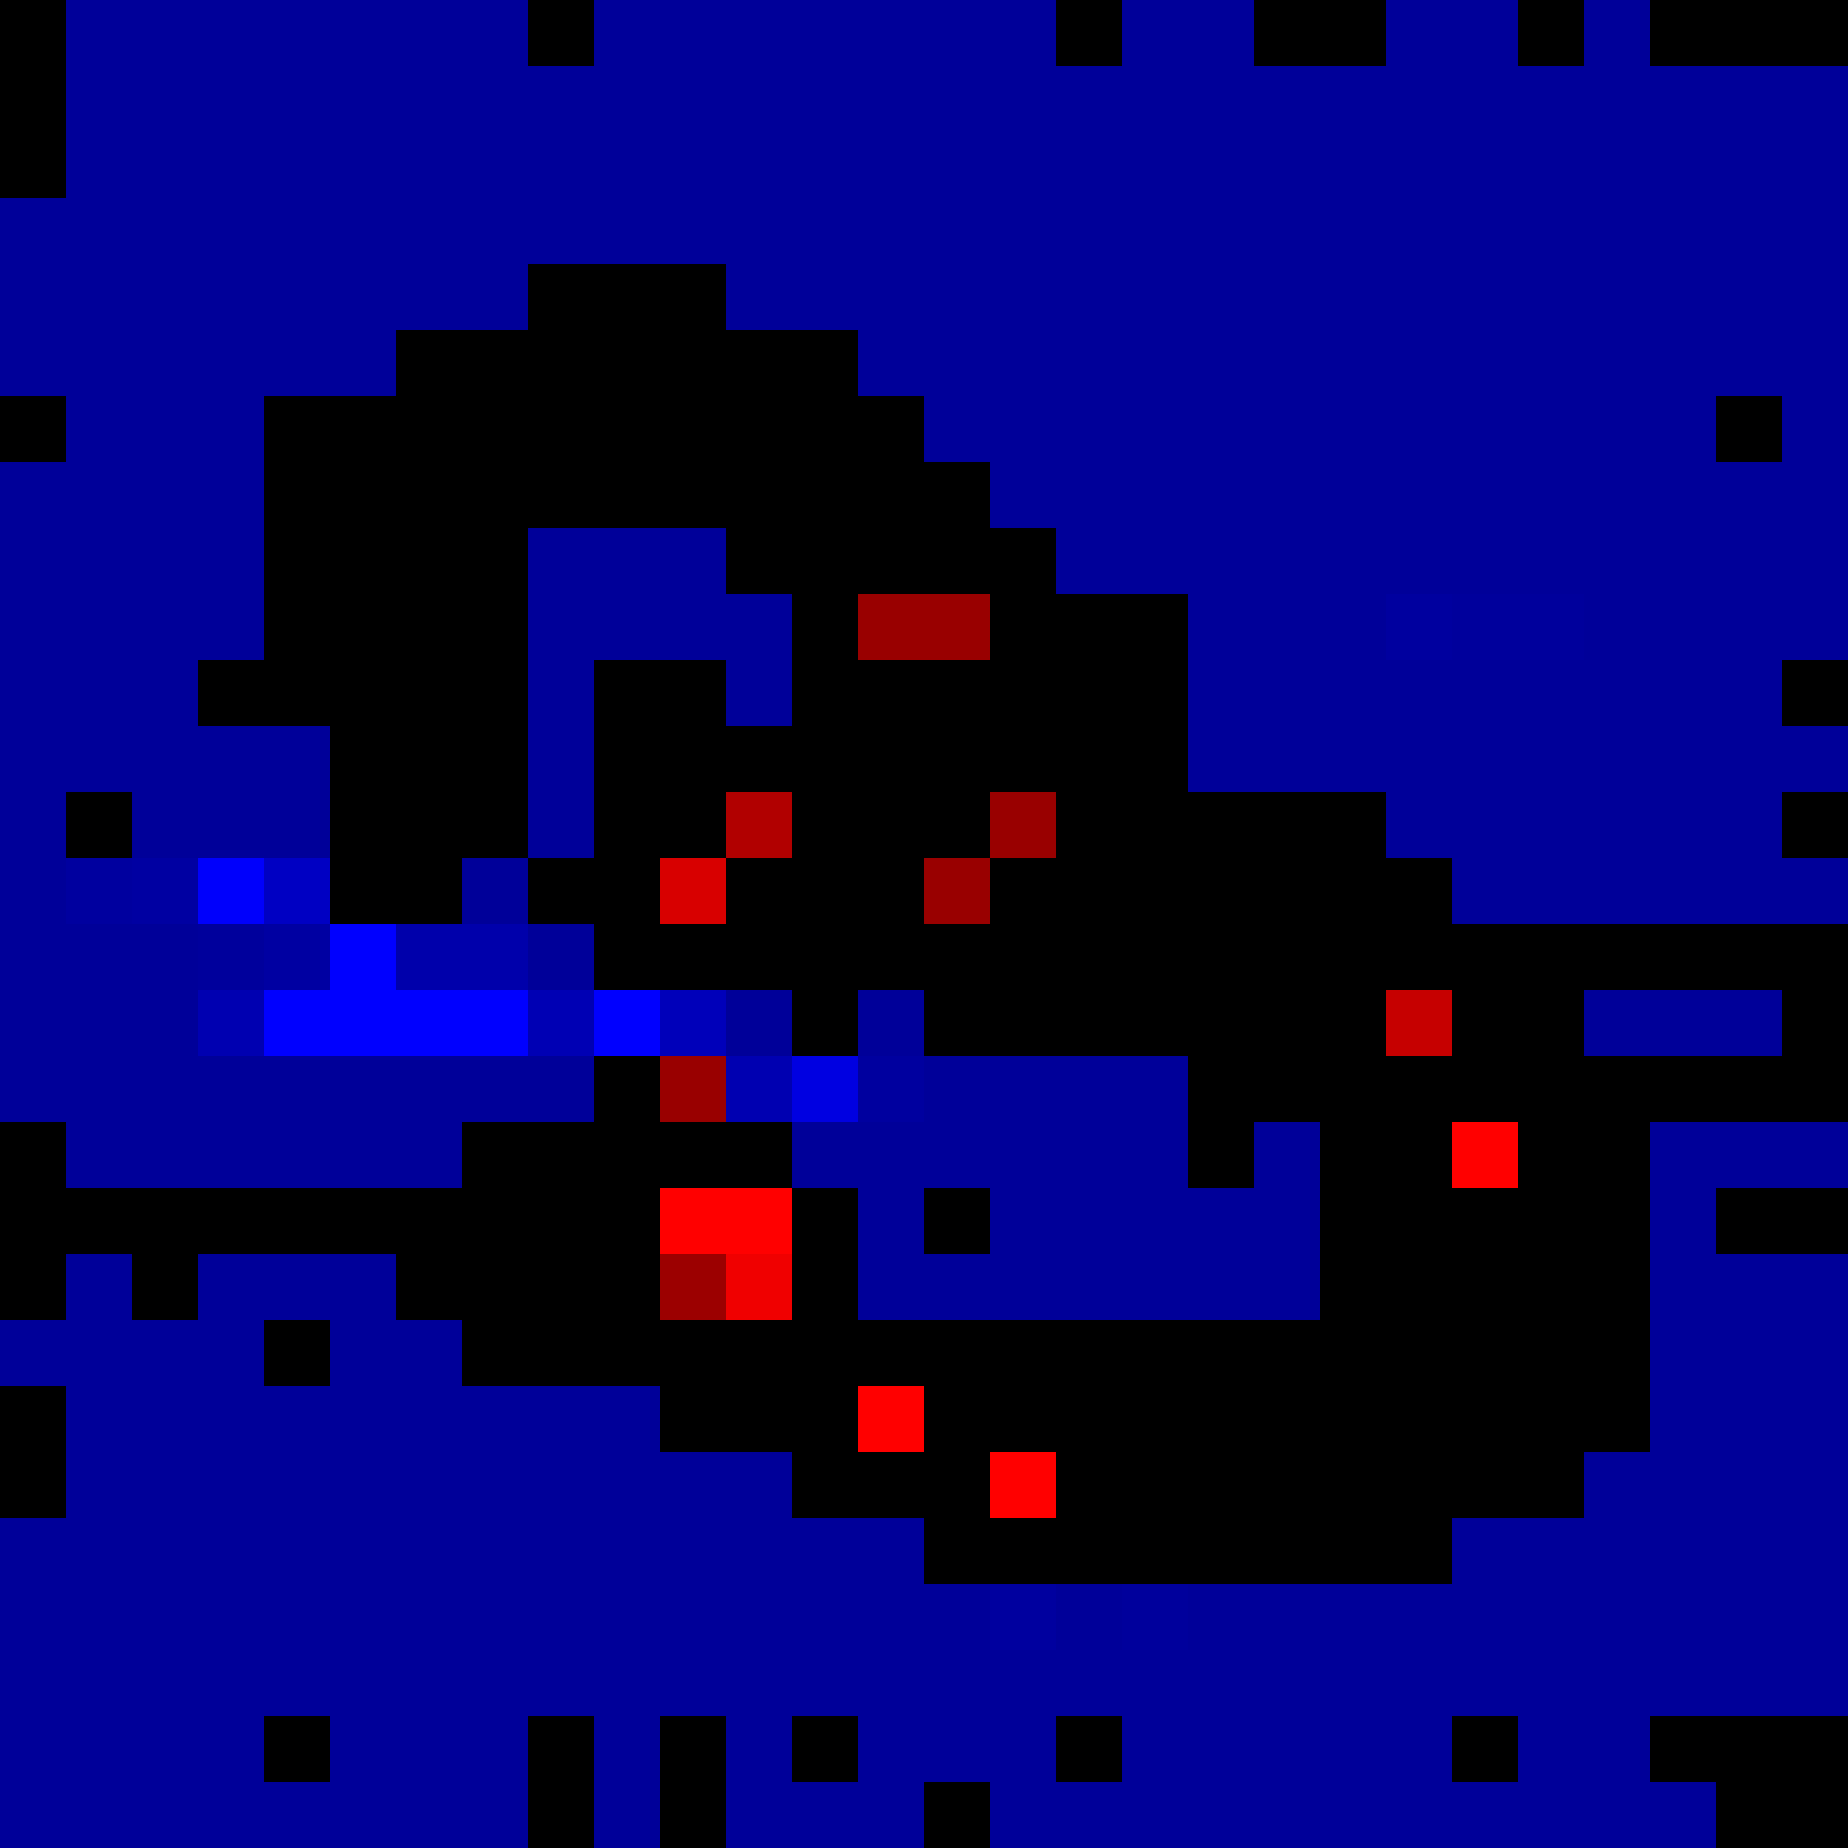
\includegraphics[width=\linewidth]{saliency/mnist_split_ic_saliency/image_030_true_3_pred_3/final_saliency_threshold_wrt_0_bright.png}\\[-1pt]{\scriptsize Logit 0}
		\end{minipage}%
		\begin{minipage}[b]{0.19\linewidth}\centering
			
\includegraphics[width=\linewidth]{saliency/mnist_split_ic_saliency/image_030_true_3_pred_3/final_saliency_threshold_wrt_1_bright.png}\\[-1pt]{\scriptsize Logit 1}
		\end{minipage}%
		\begin{minipage}[b]{0.19\linewidth}\centering
			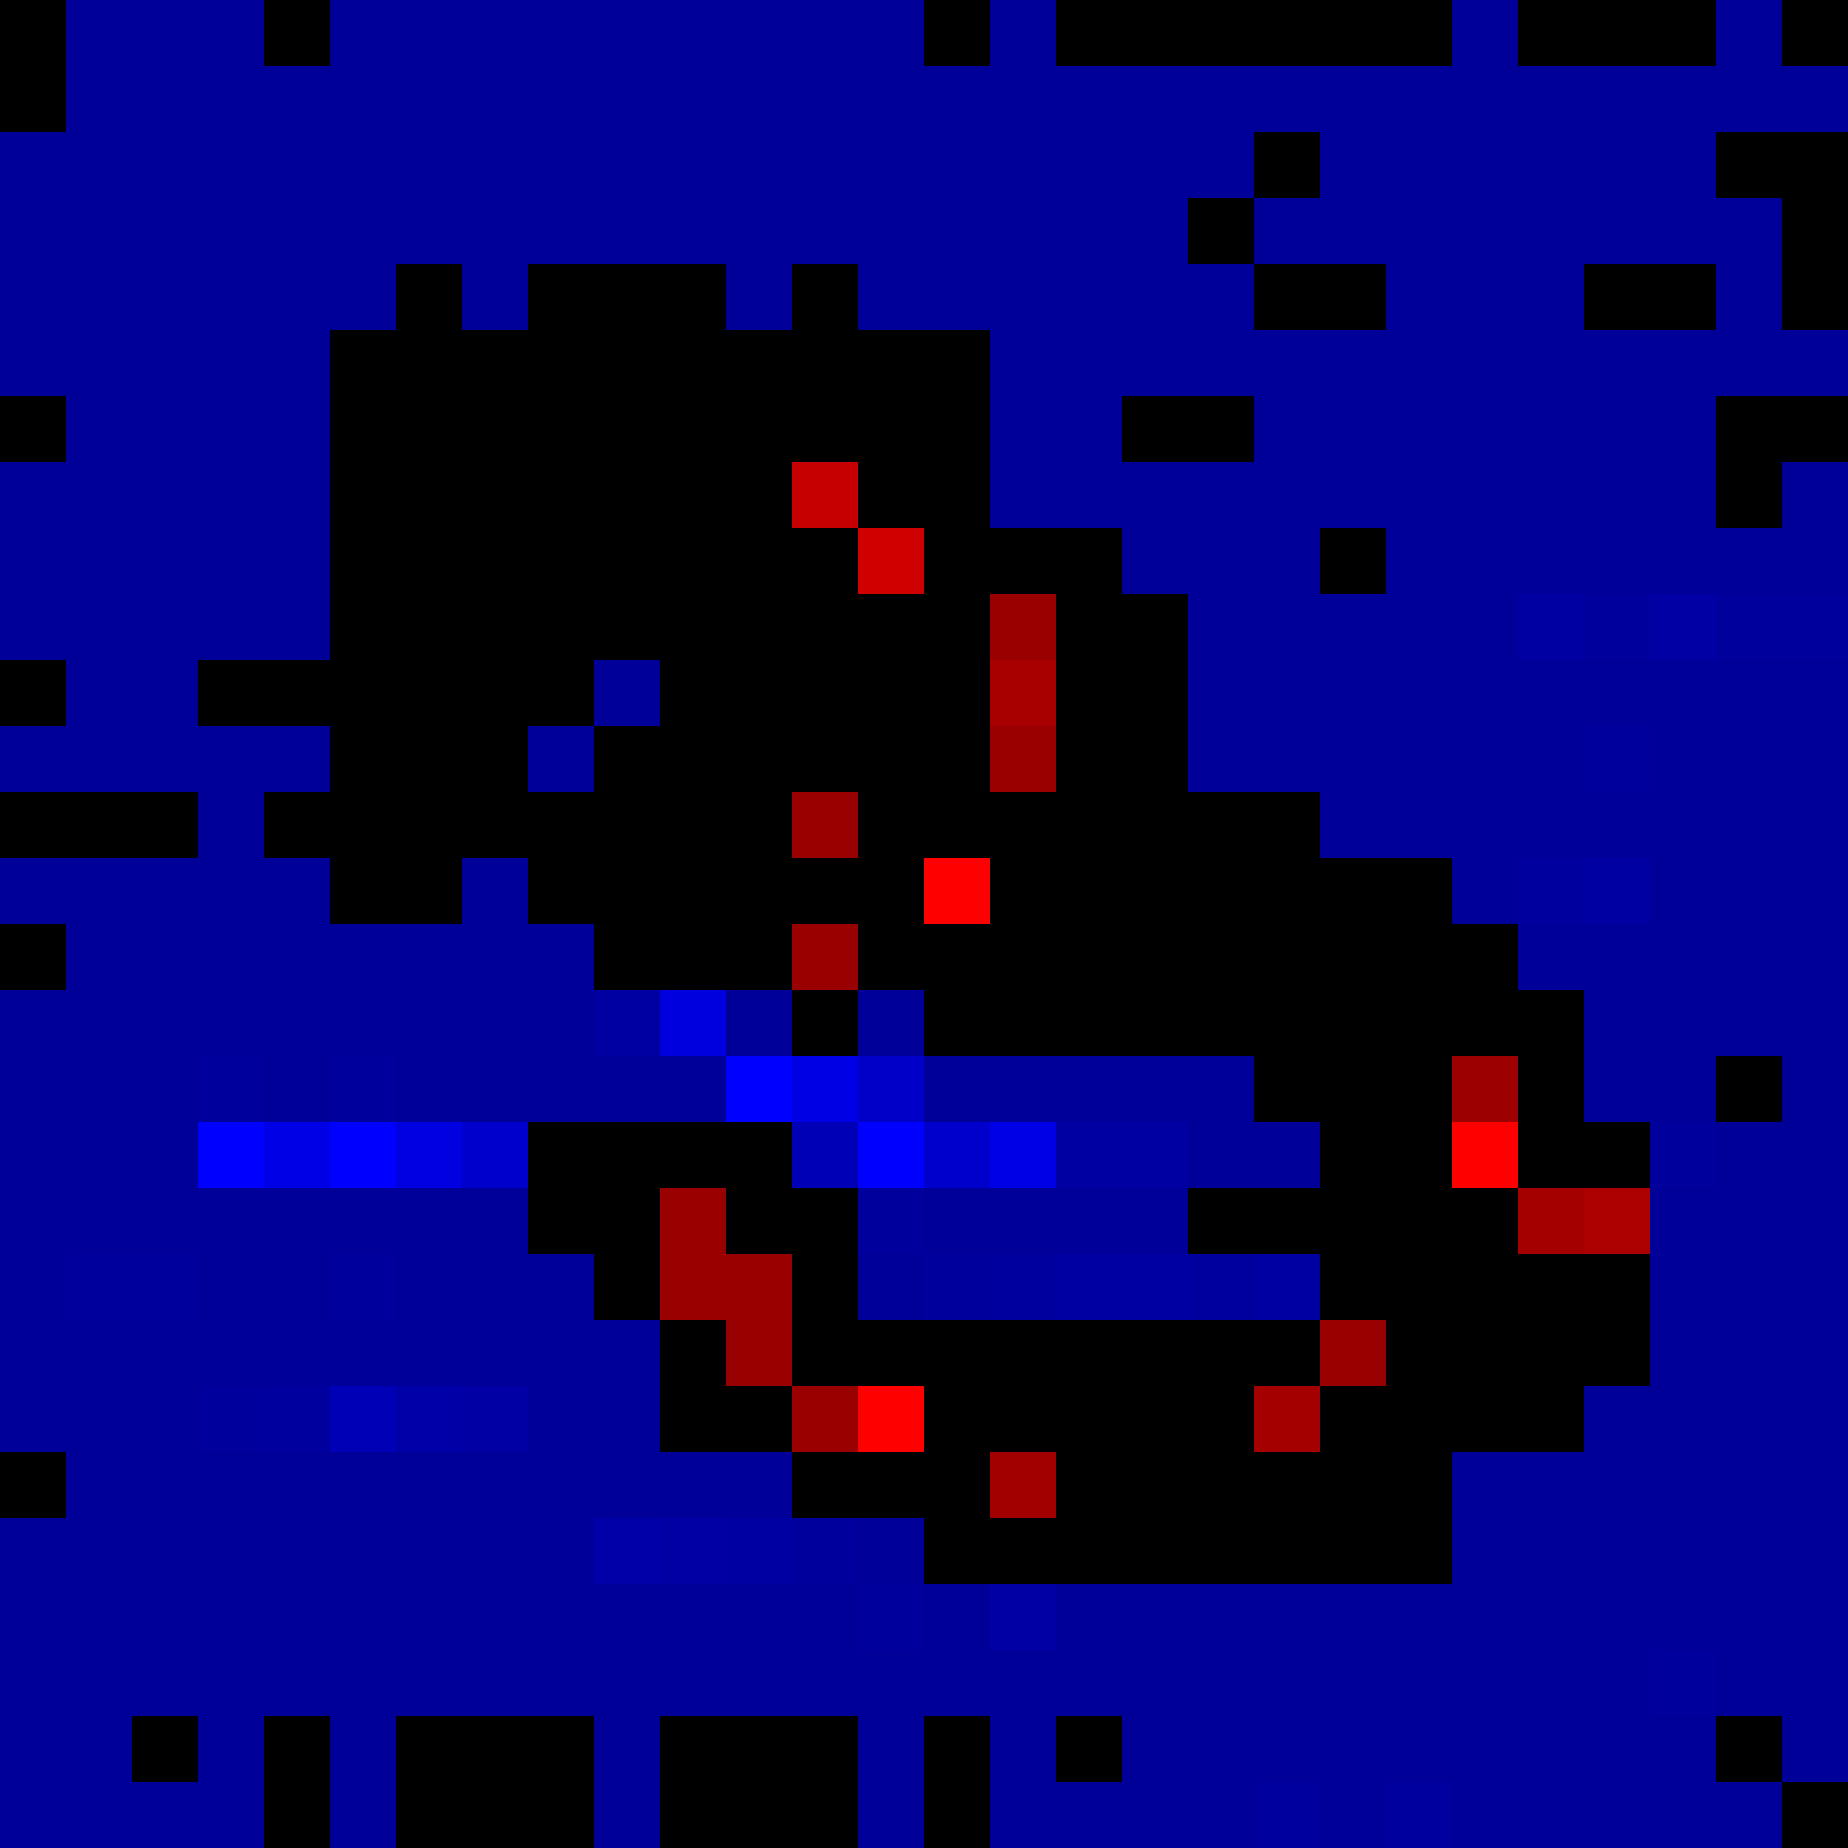
\includegraphics[width=\linewidth]{saliency/mnist_split_ic_saliency/image_030_true_3_pred_3/final_saliency_threshold_wrt_2_bright.png}\\[-1pt]{\scriptsize Logit 2}
		\end{minipage}%
		\begin{minipage}[b]{0.19\linewidth}\centering
			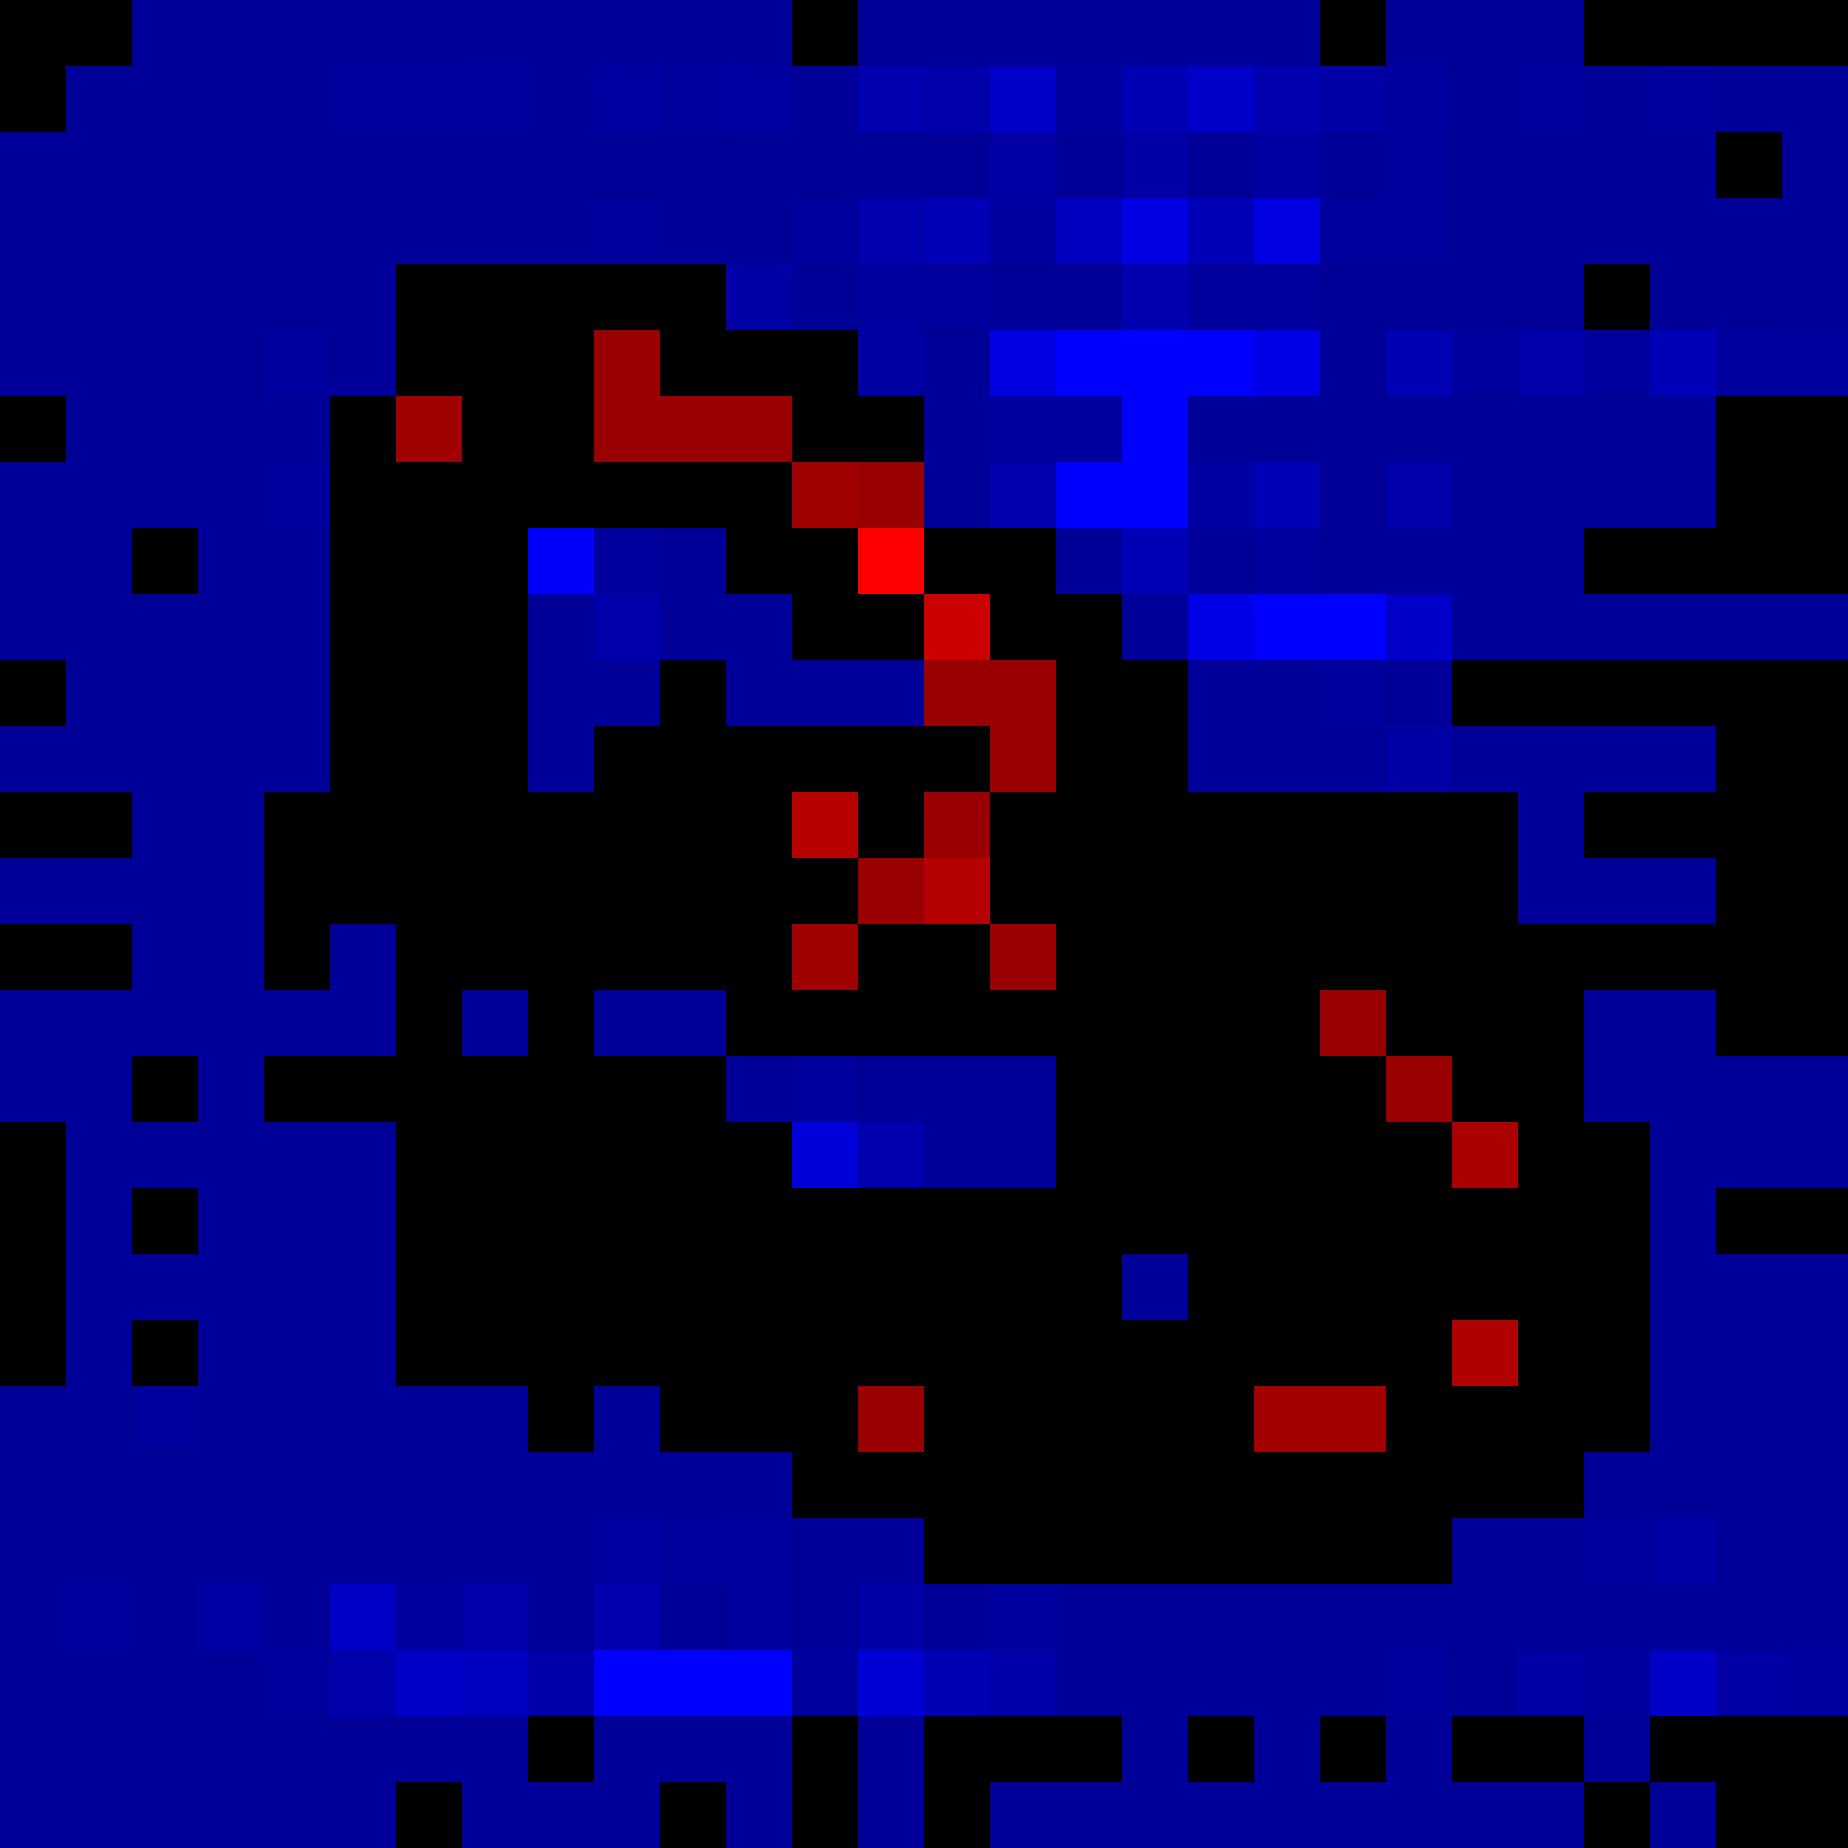
\includegraphics[width=\linewidth]{saliency/mnist_split_ic_saliency/image_030_true_3_pred_3/final_saliency_threshold_wrt_3_bright.png}\\[-1pt]{\scriptsize Logit 3}
		\end{minipage}%
		\begin{minipage}[b]{0.19\linewidth}\centering
			
\includegraphics[width=\linewidth]{saliency/mnist_split_ic_saliency/image_030_true_3_pred_3/final_saliency_threshold_wrt_4_bright.png}\\[-1pt]{\scriptsize Logit 4}
		\end{minipage}

		\vspace{0.12cm}

		\begin{minipage}[b]{0.19\linewidth}\centering
			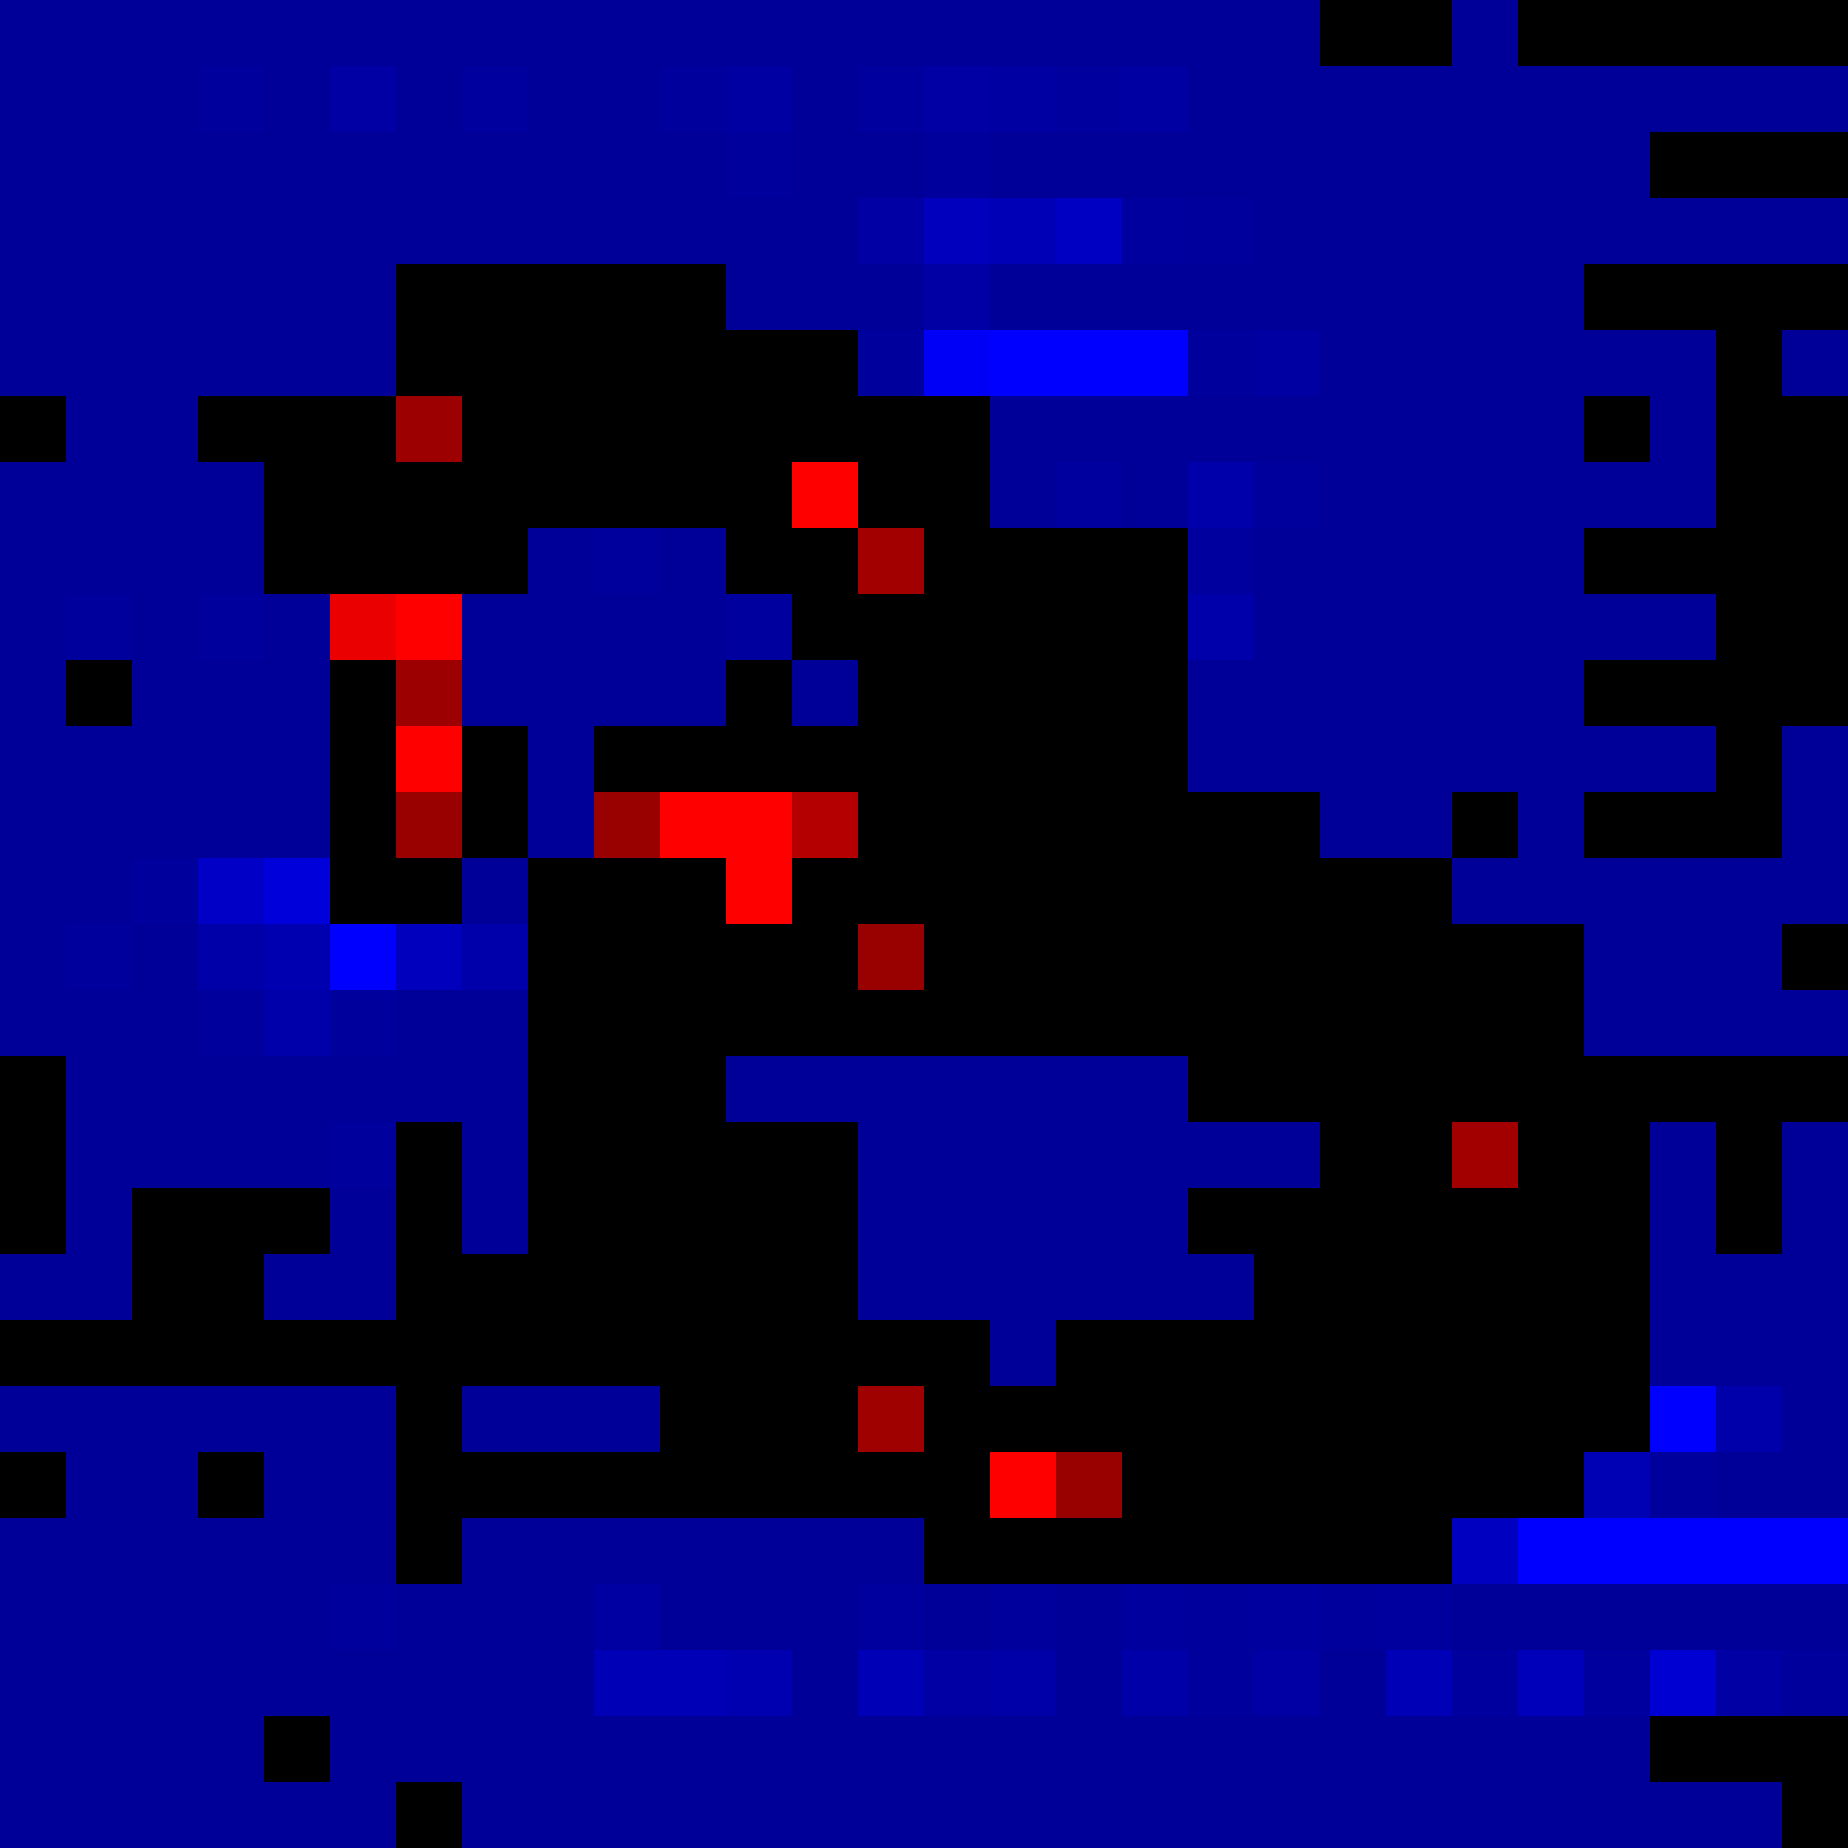
\includegraphics[width=\linewidth]{saliency/mnist_split_ic_saliency/image_030_true_3_pred_3/final_saliency_threshold_wrt_5_bright.png}\\[-1pt]{\scriptsize Logit 5}
		\end{minipage}%
		\begin{minipage}[b]{0.19\linewidth}\centering
			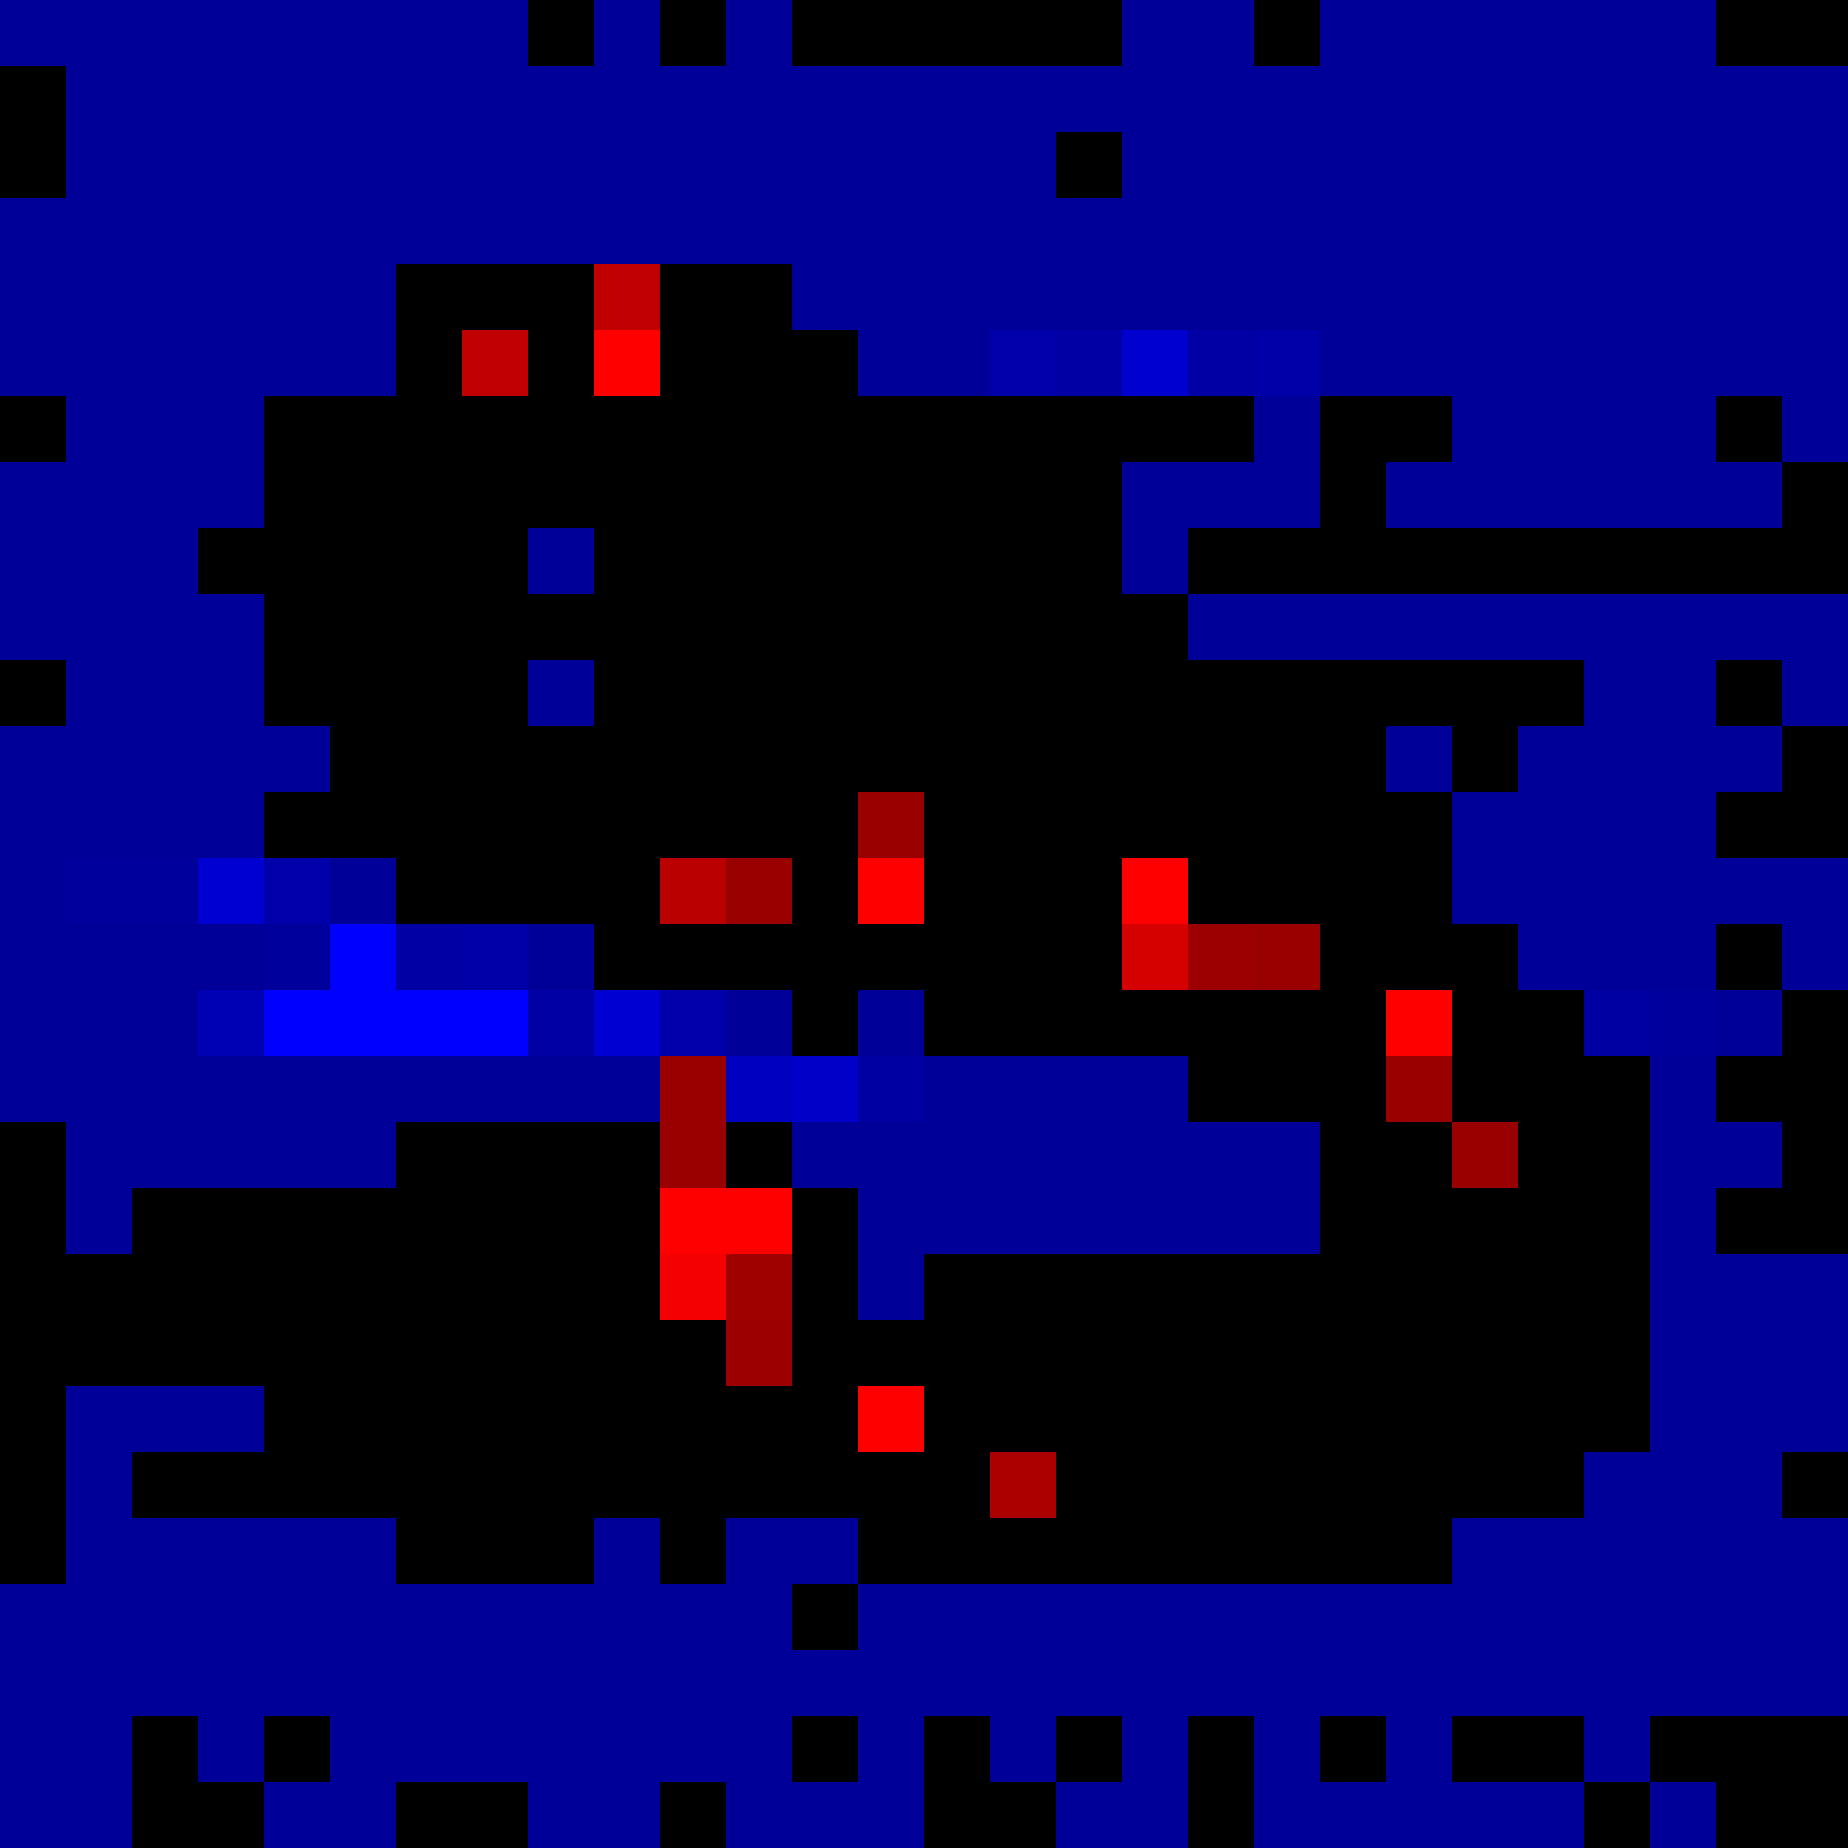
\includegraphics[width=\linewidth]{saliency/mnist_split_ic_saliency/image_030_true_3_pred_3/final_saliency_threshold_wrt_6_bright.png}\\[-1pt]{\scriptsize Logit 6}
		\end{minipage}%
		\begin{minipage}[b]{0.19\linewidth}\centering
			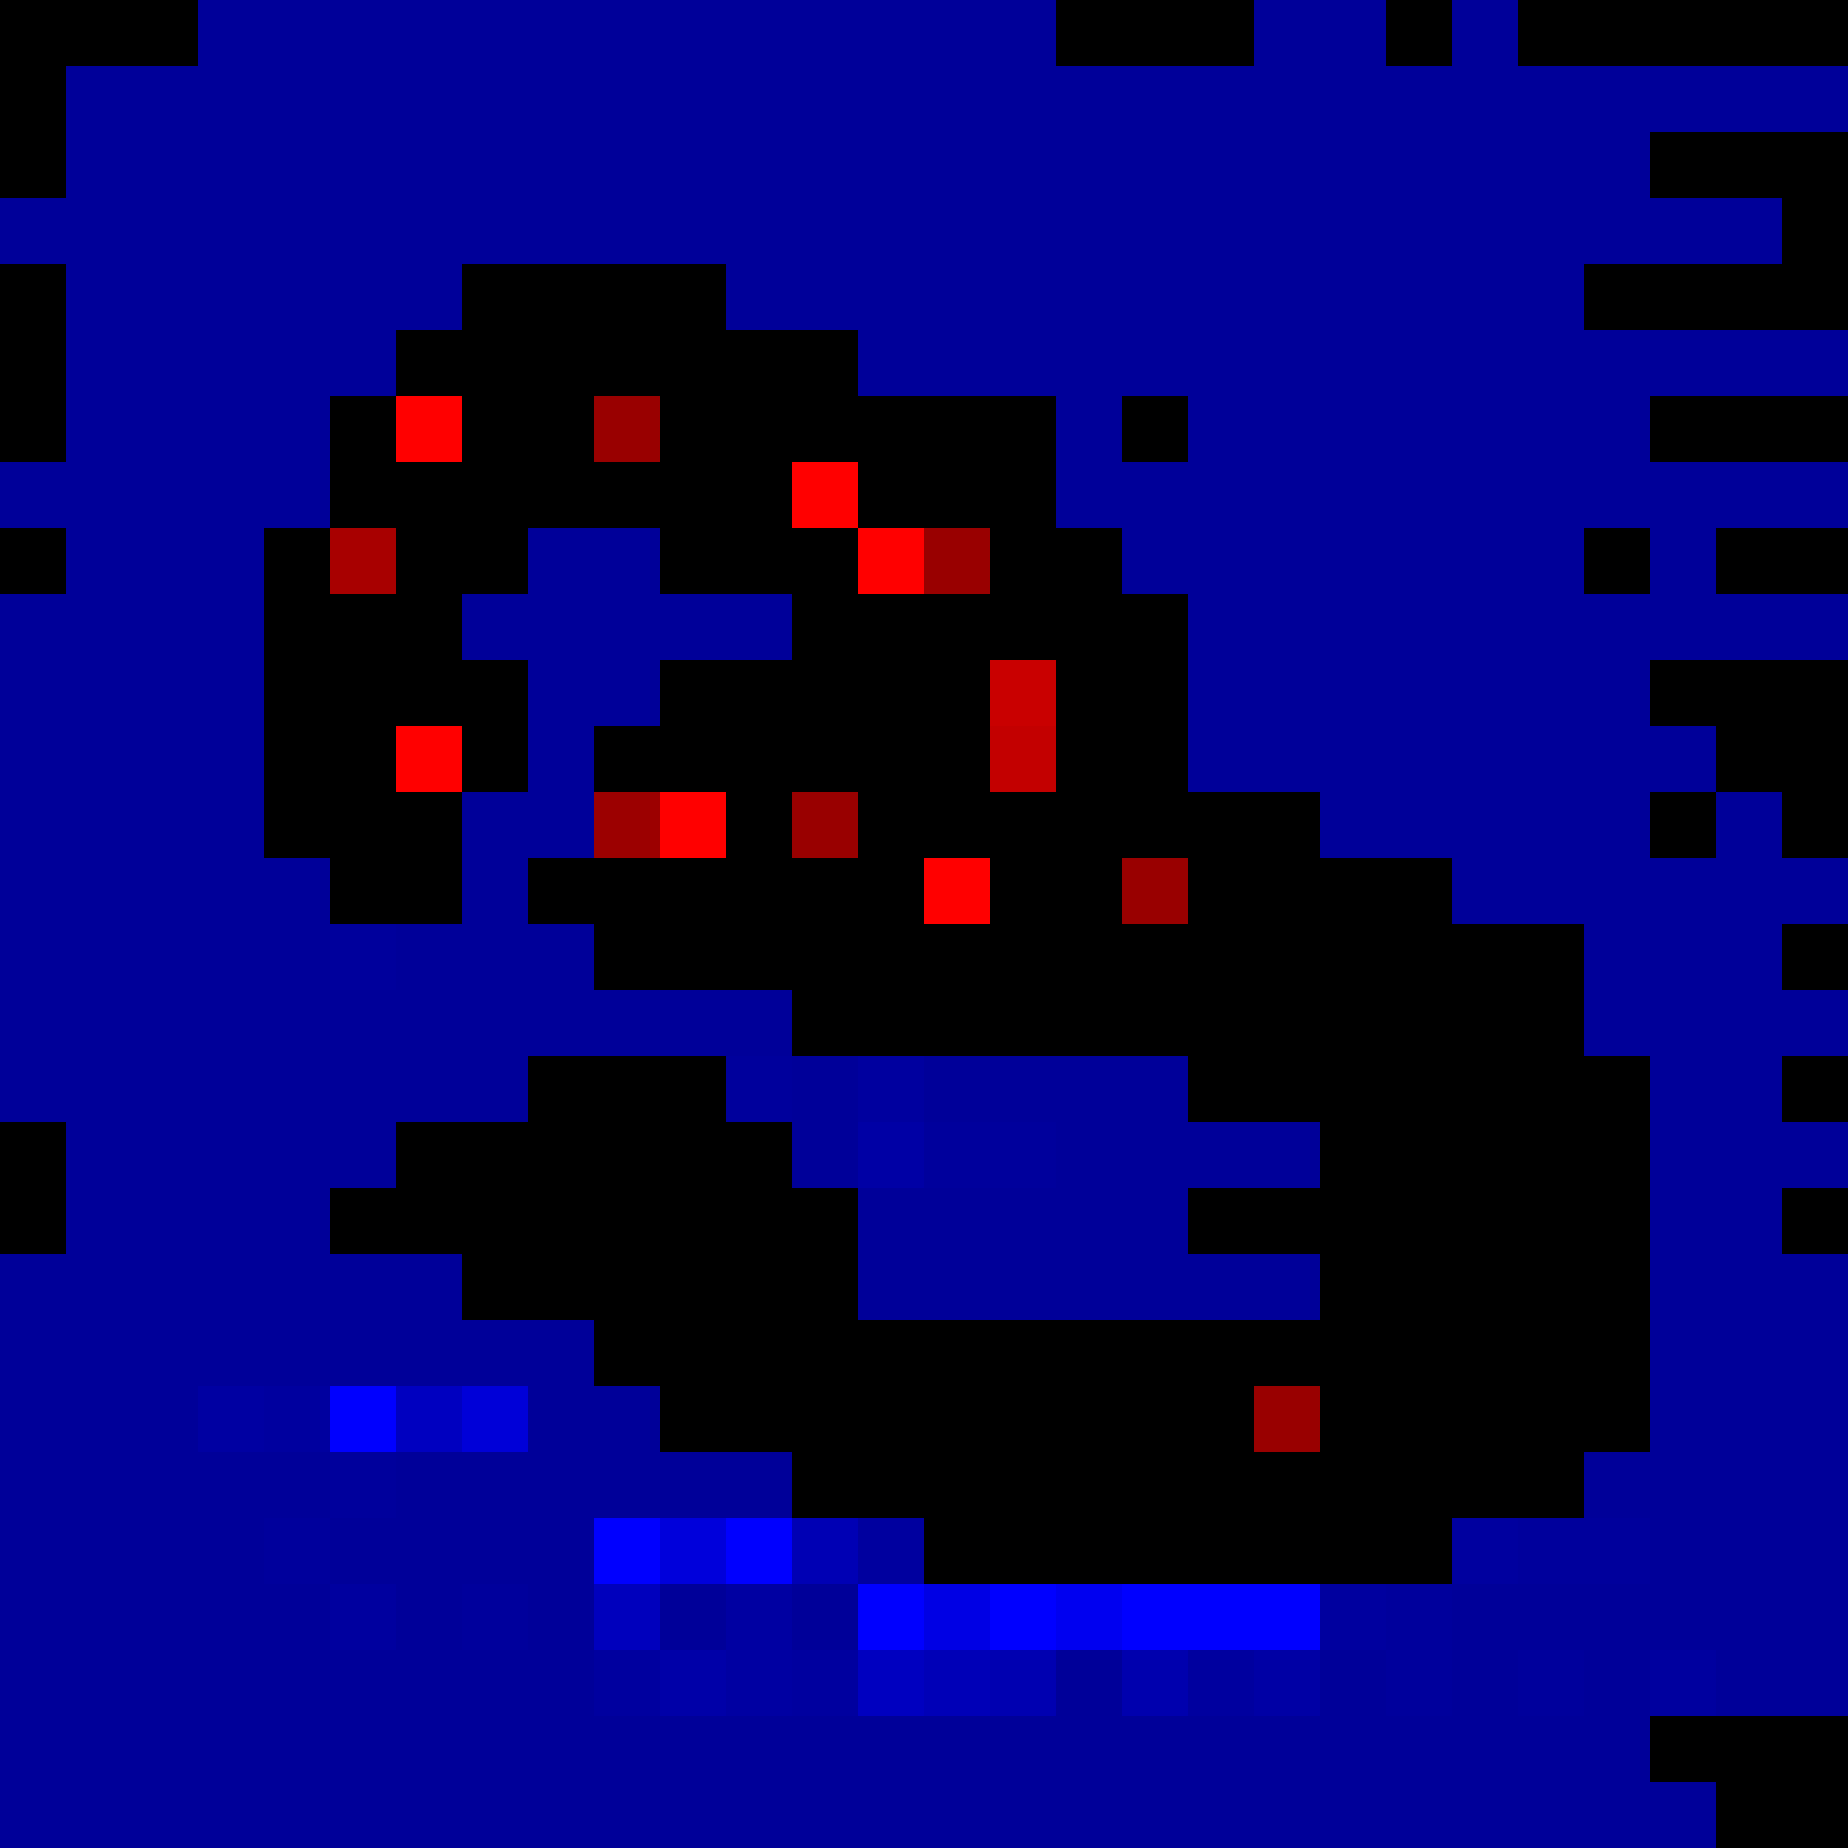
\includegraphics[width=\linewidth]{saliency/mnist_split_ic_saliency/image_030_true_3_pred_3/final_saliency_threshold_wrt_7_bright.png}\\[-1pt]{\scriptsize Logit 7}
		\end{minipage}%
		\begin{minipage}[b]{0.19\linewidth}\centering
			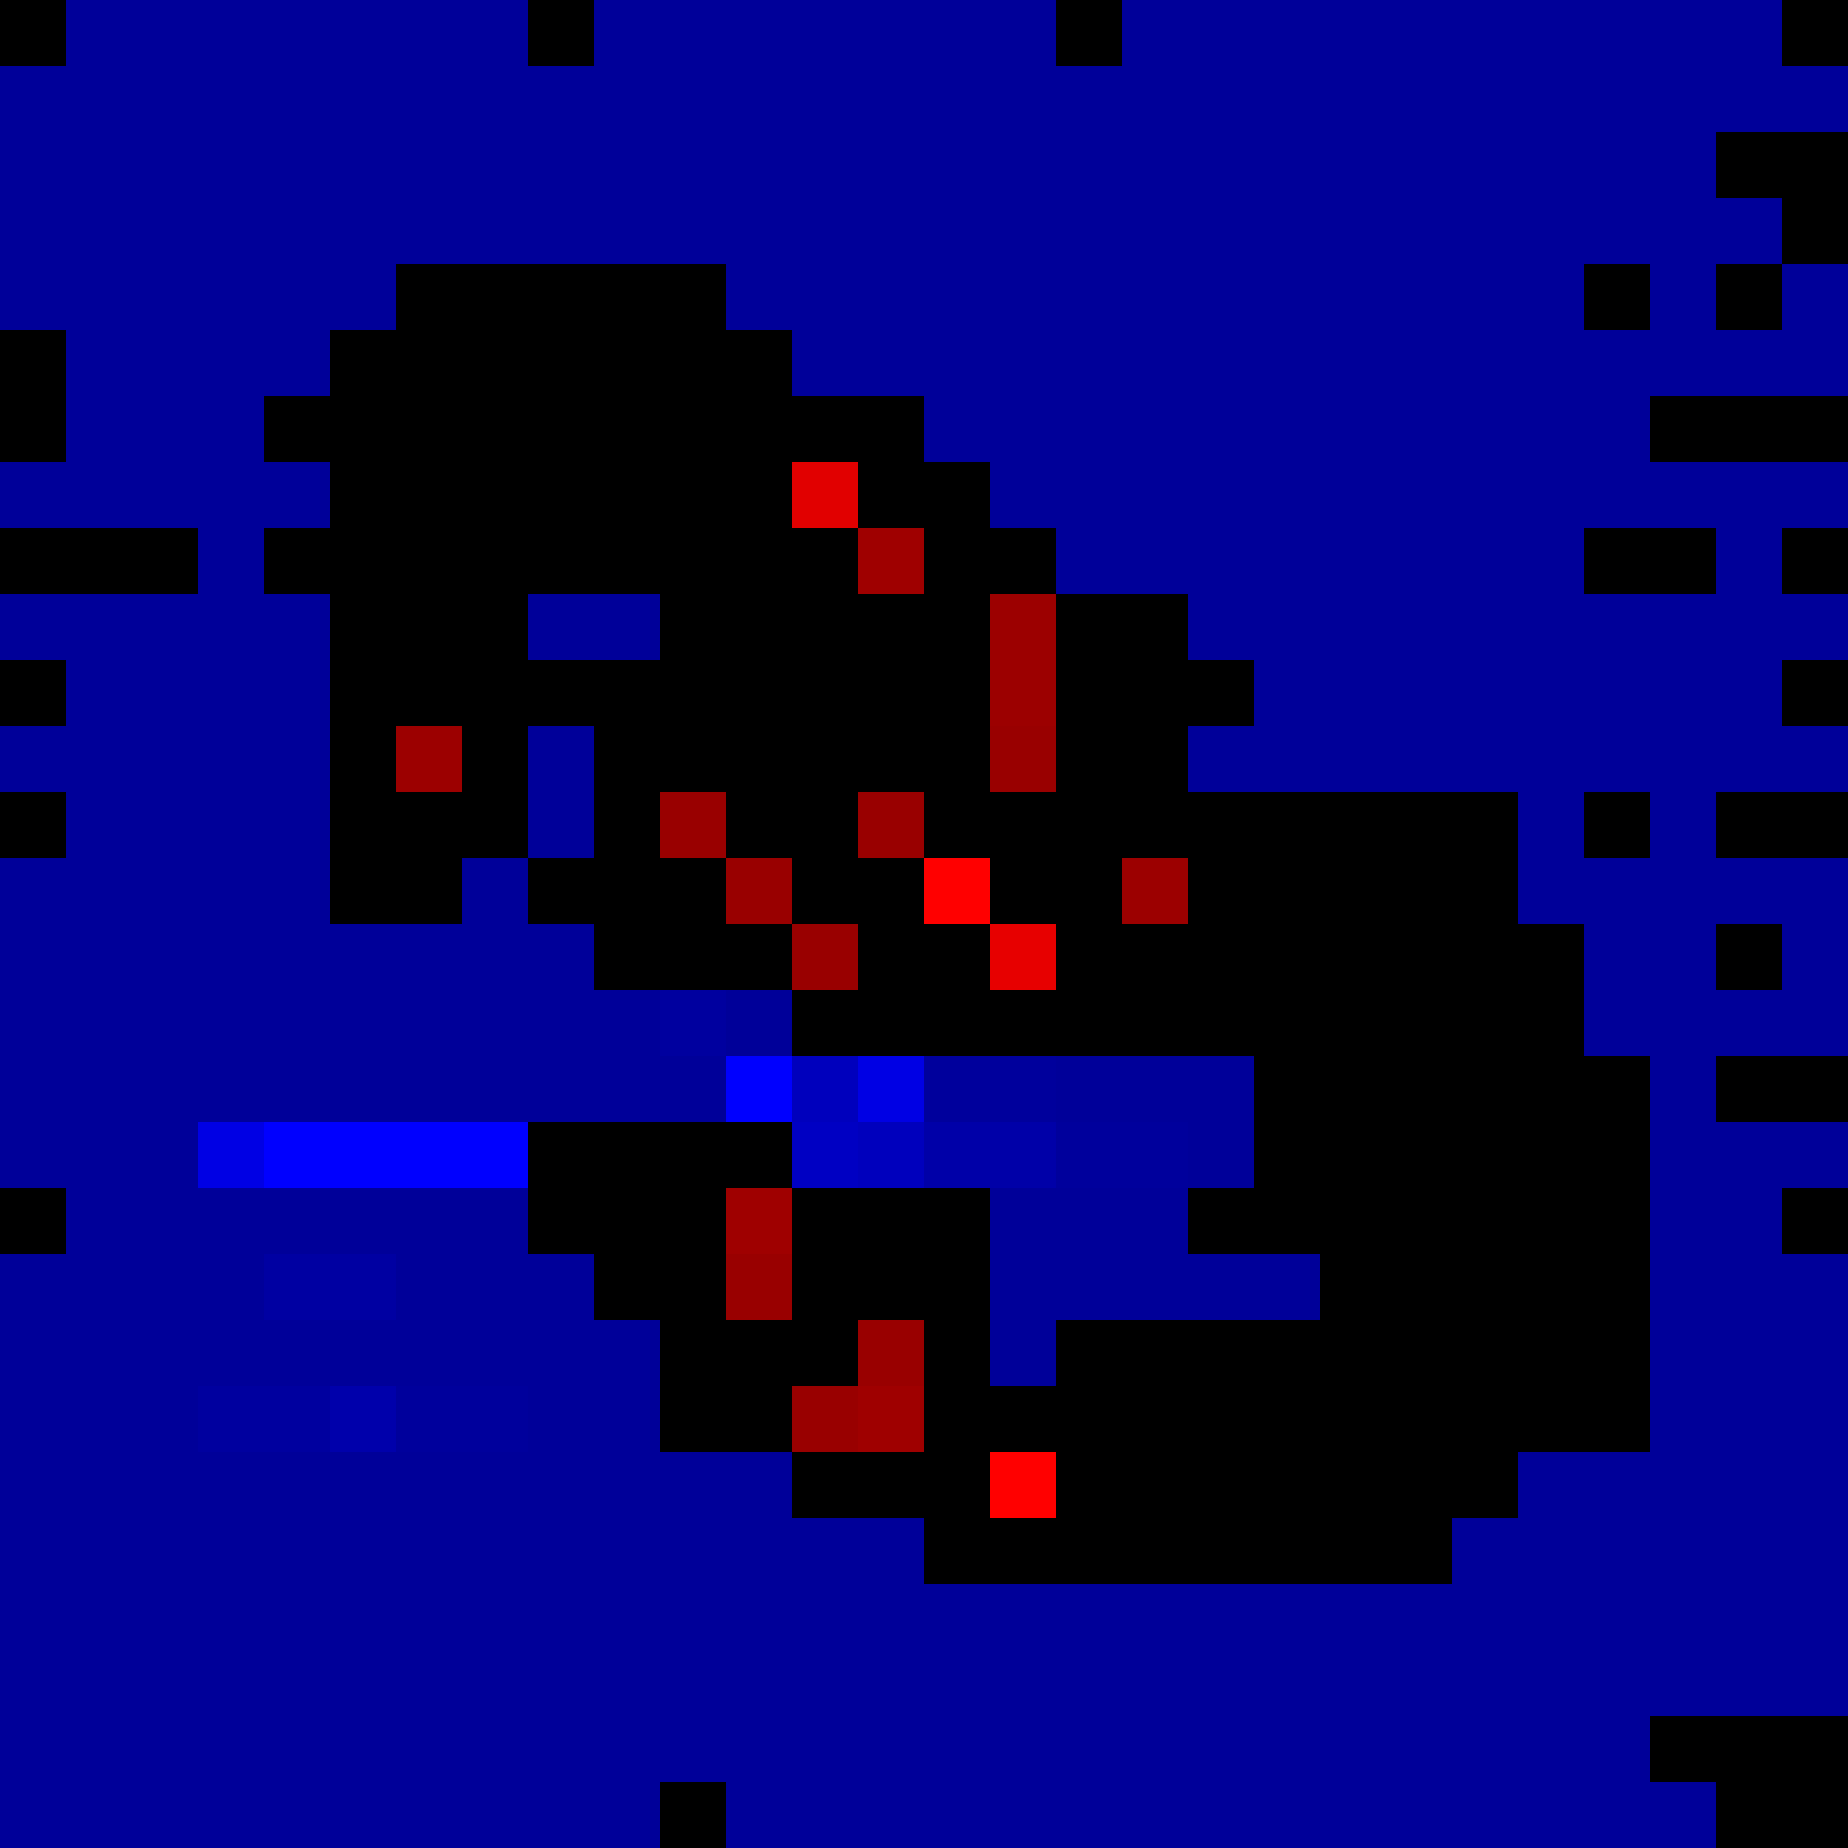
\includegraphics[width=\linewidth]{saliency/mnist_split_ic_saliency/image_030_true_3_pred_3/final_saliency_threshold_wrt_8_bright.png}\\[-1pt]{\scriptsize Logit 8}
		\end{minipage}%
		\begin{minipage}[b]{0.19\linewidth}\centering
			
\includegraphics[width=\linewidth]{saliency/mnist_split_ic_saliency/image_030_true_3_pred_3/final_saliency_threshold_wrt_9_bright.png}\\[-1pt]{\scriptsize Logit 9}
		\end{minipage}
	\end{minipage}
	}%
\caption[Stream gradients of the inverted-input DIC model]{Stream gradients of the inverted-input DIC model (\texttt{cnn\_maxout} DICIN) on a correctly classified MNIST test digit ``3'', thresholded and overlaid per class logit. The $g$-stream gradient (red) highlights sensitivities on present strokes, while the $h$-stream gradient (blue) highlights sensitivities at candidate missing-stroke locations. These stream-local maps do not by themselves establish the effect of adding pixels on the complete model. Left: the original digit.}
	\label{fig:mnist_split_ic_saliency}
\end{figure}

\begin{figure}[t]
\QualitativeImageContent{
	\centering
	\begin{minipage}[c]{0.15\linewidth}
		\centering
		
\includegraphics[width=\linewidth]{saliency/mnist_split_ic_saliency/image_036_true_3_pred_3/original.png}\\[-1pt]
		{\scriptsize Original}
	\end{minipage}\hspace{0.015\linewidth}%
	\begin{minipage}[c]{0.80\linewidth}
		\centering
		\begin{minipage}[b]{0.19\linewidth}\centering
			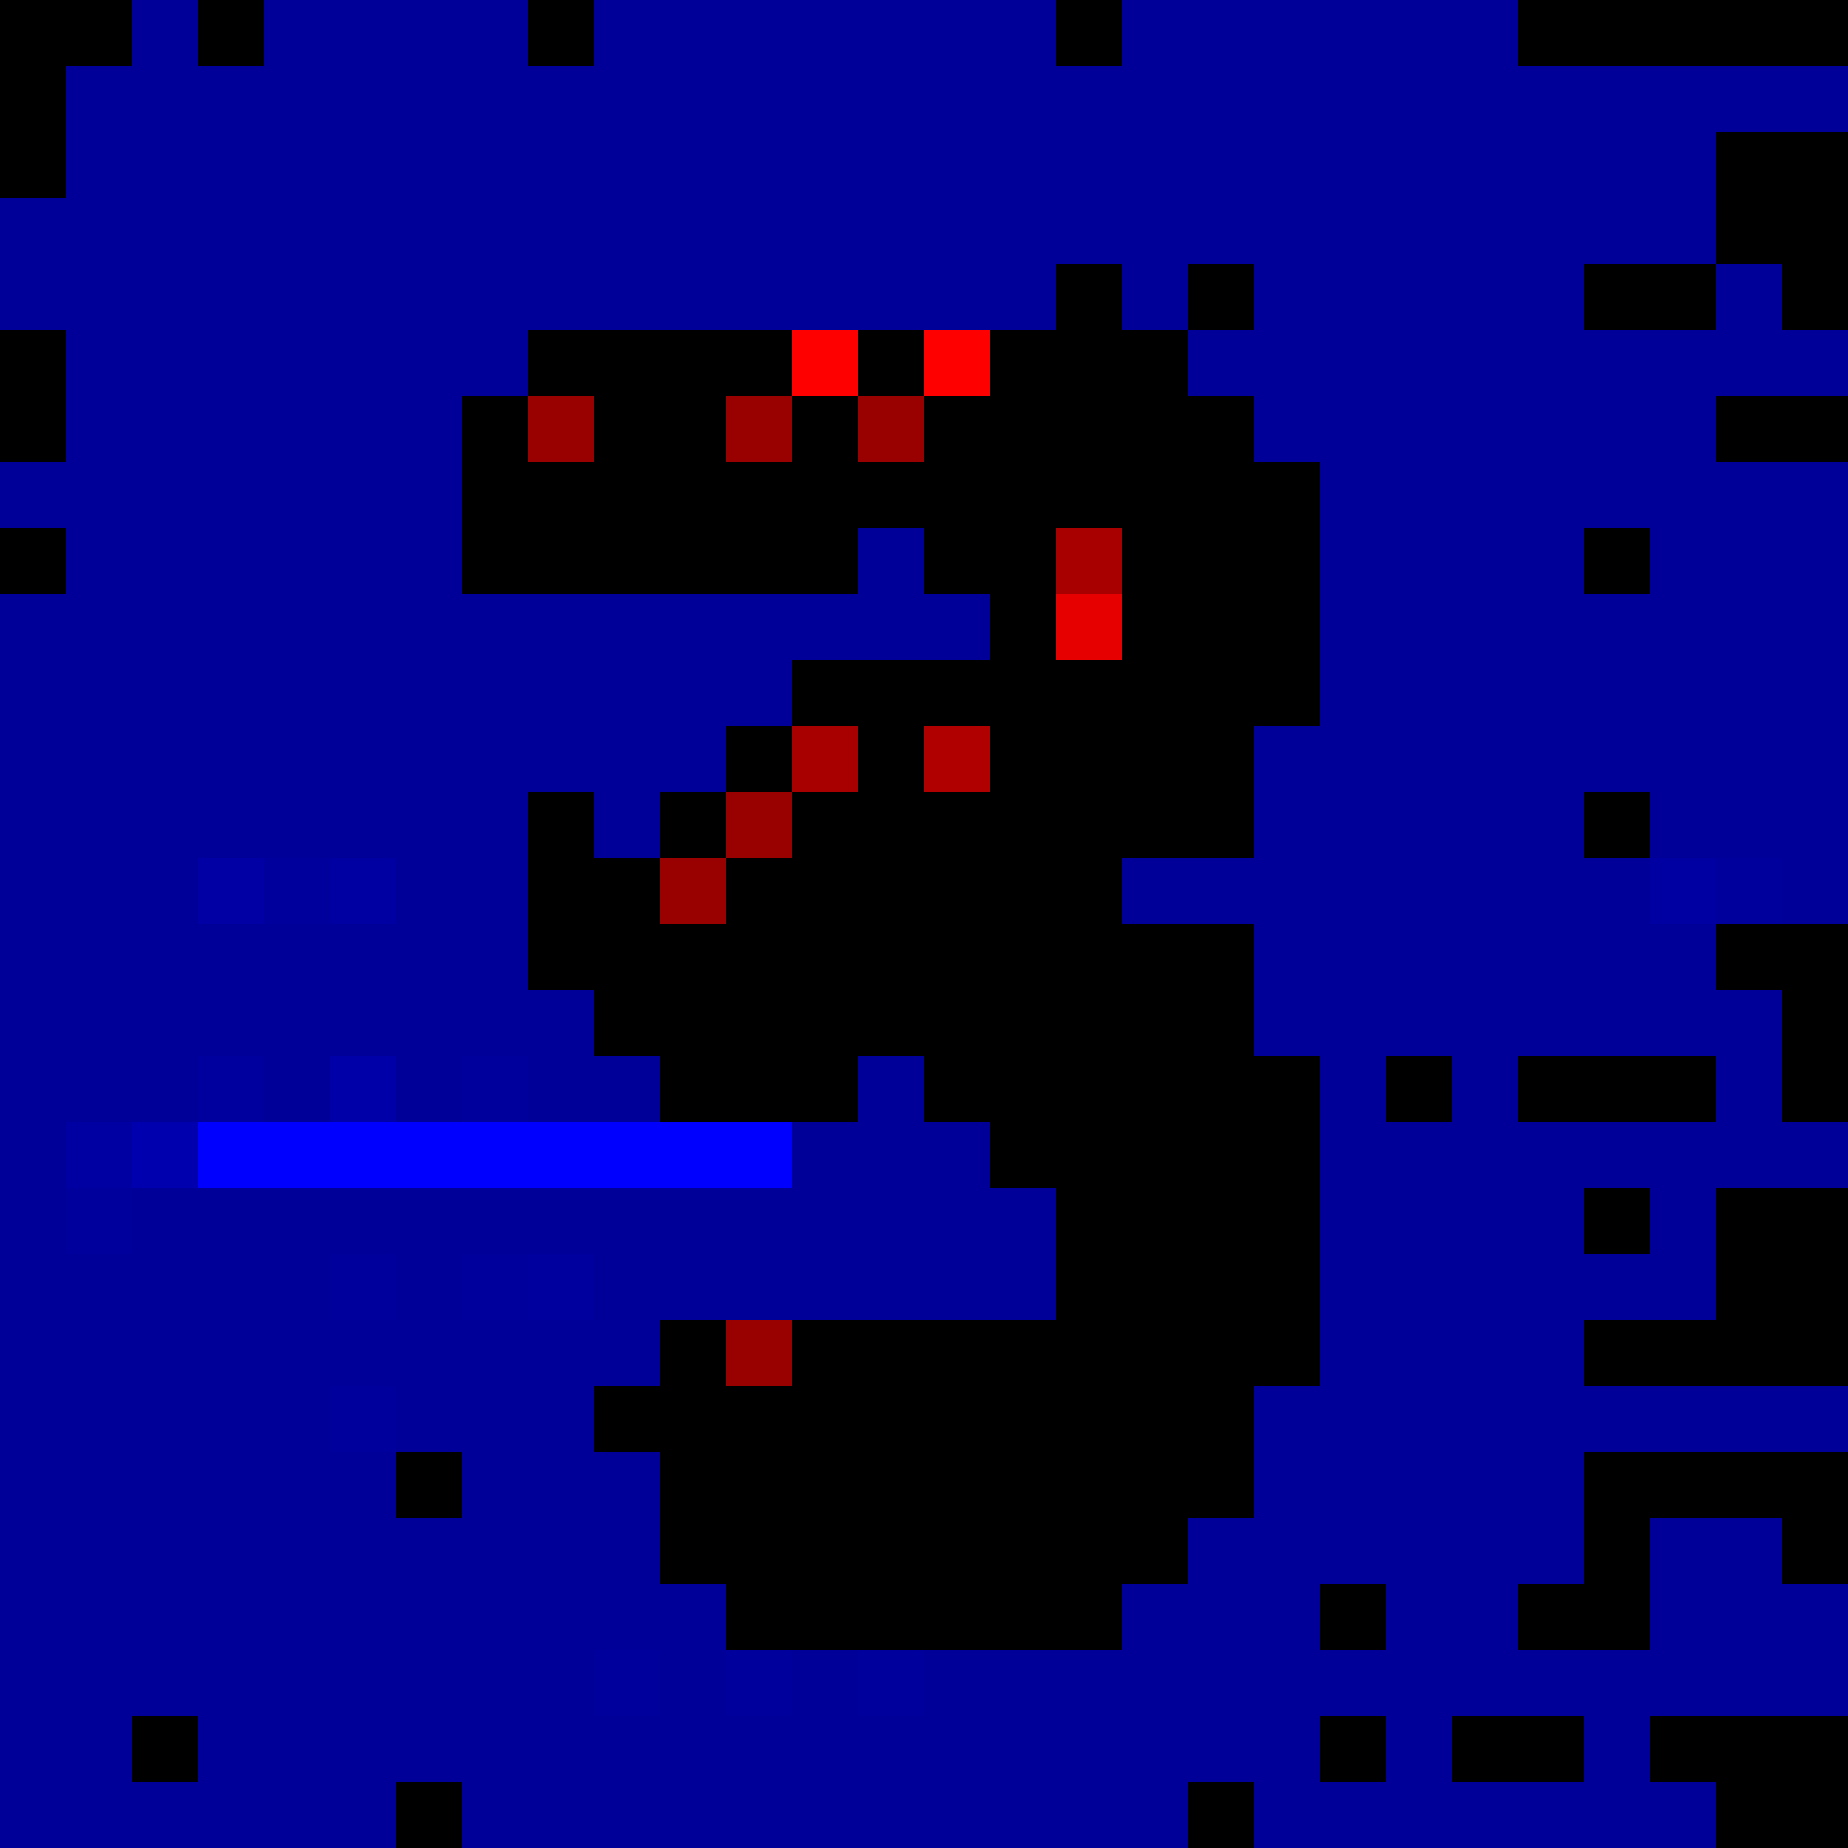
\includegraphics[width=\linewidth]{saliency/mnist_split_ic_saliency/image_036_true_3_pred_3/final_saliency_threshold_wrt_0_bright.png}\\[-1pt]{\scriptsize Logit 0}
		\end{minipage}%
		\begin{minipage}[b]{0.19\linewidth}\centering
			
\includegraphics[width=\linewidth]{saliency/mnist_split_ic_saliency/image_036_true_3_pred_3/final_saliency_threshold_wrt_1_bright.png}\\[-1pt]{\scriptsize Logit 1}
		\end{minipage}%
		\begin{minipage}[b]{0.19\linewidth}\centering
			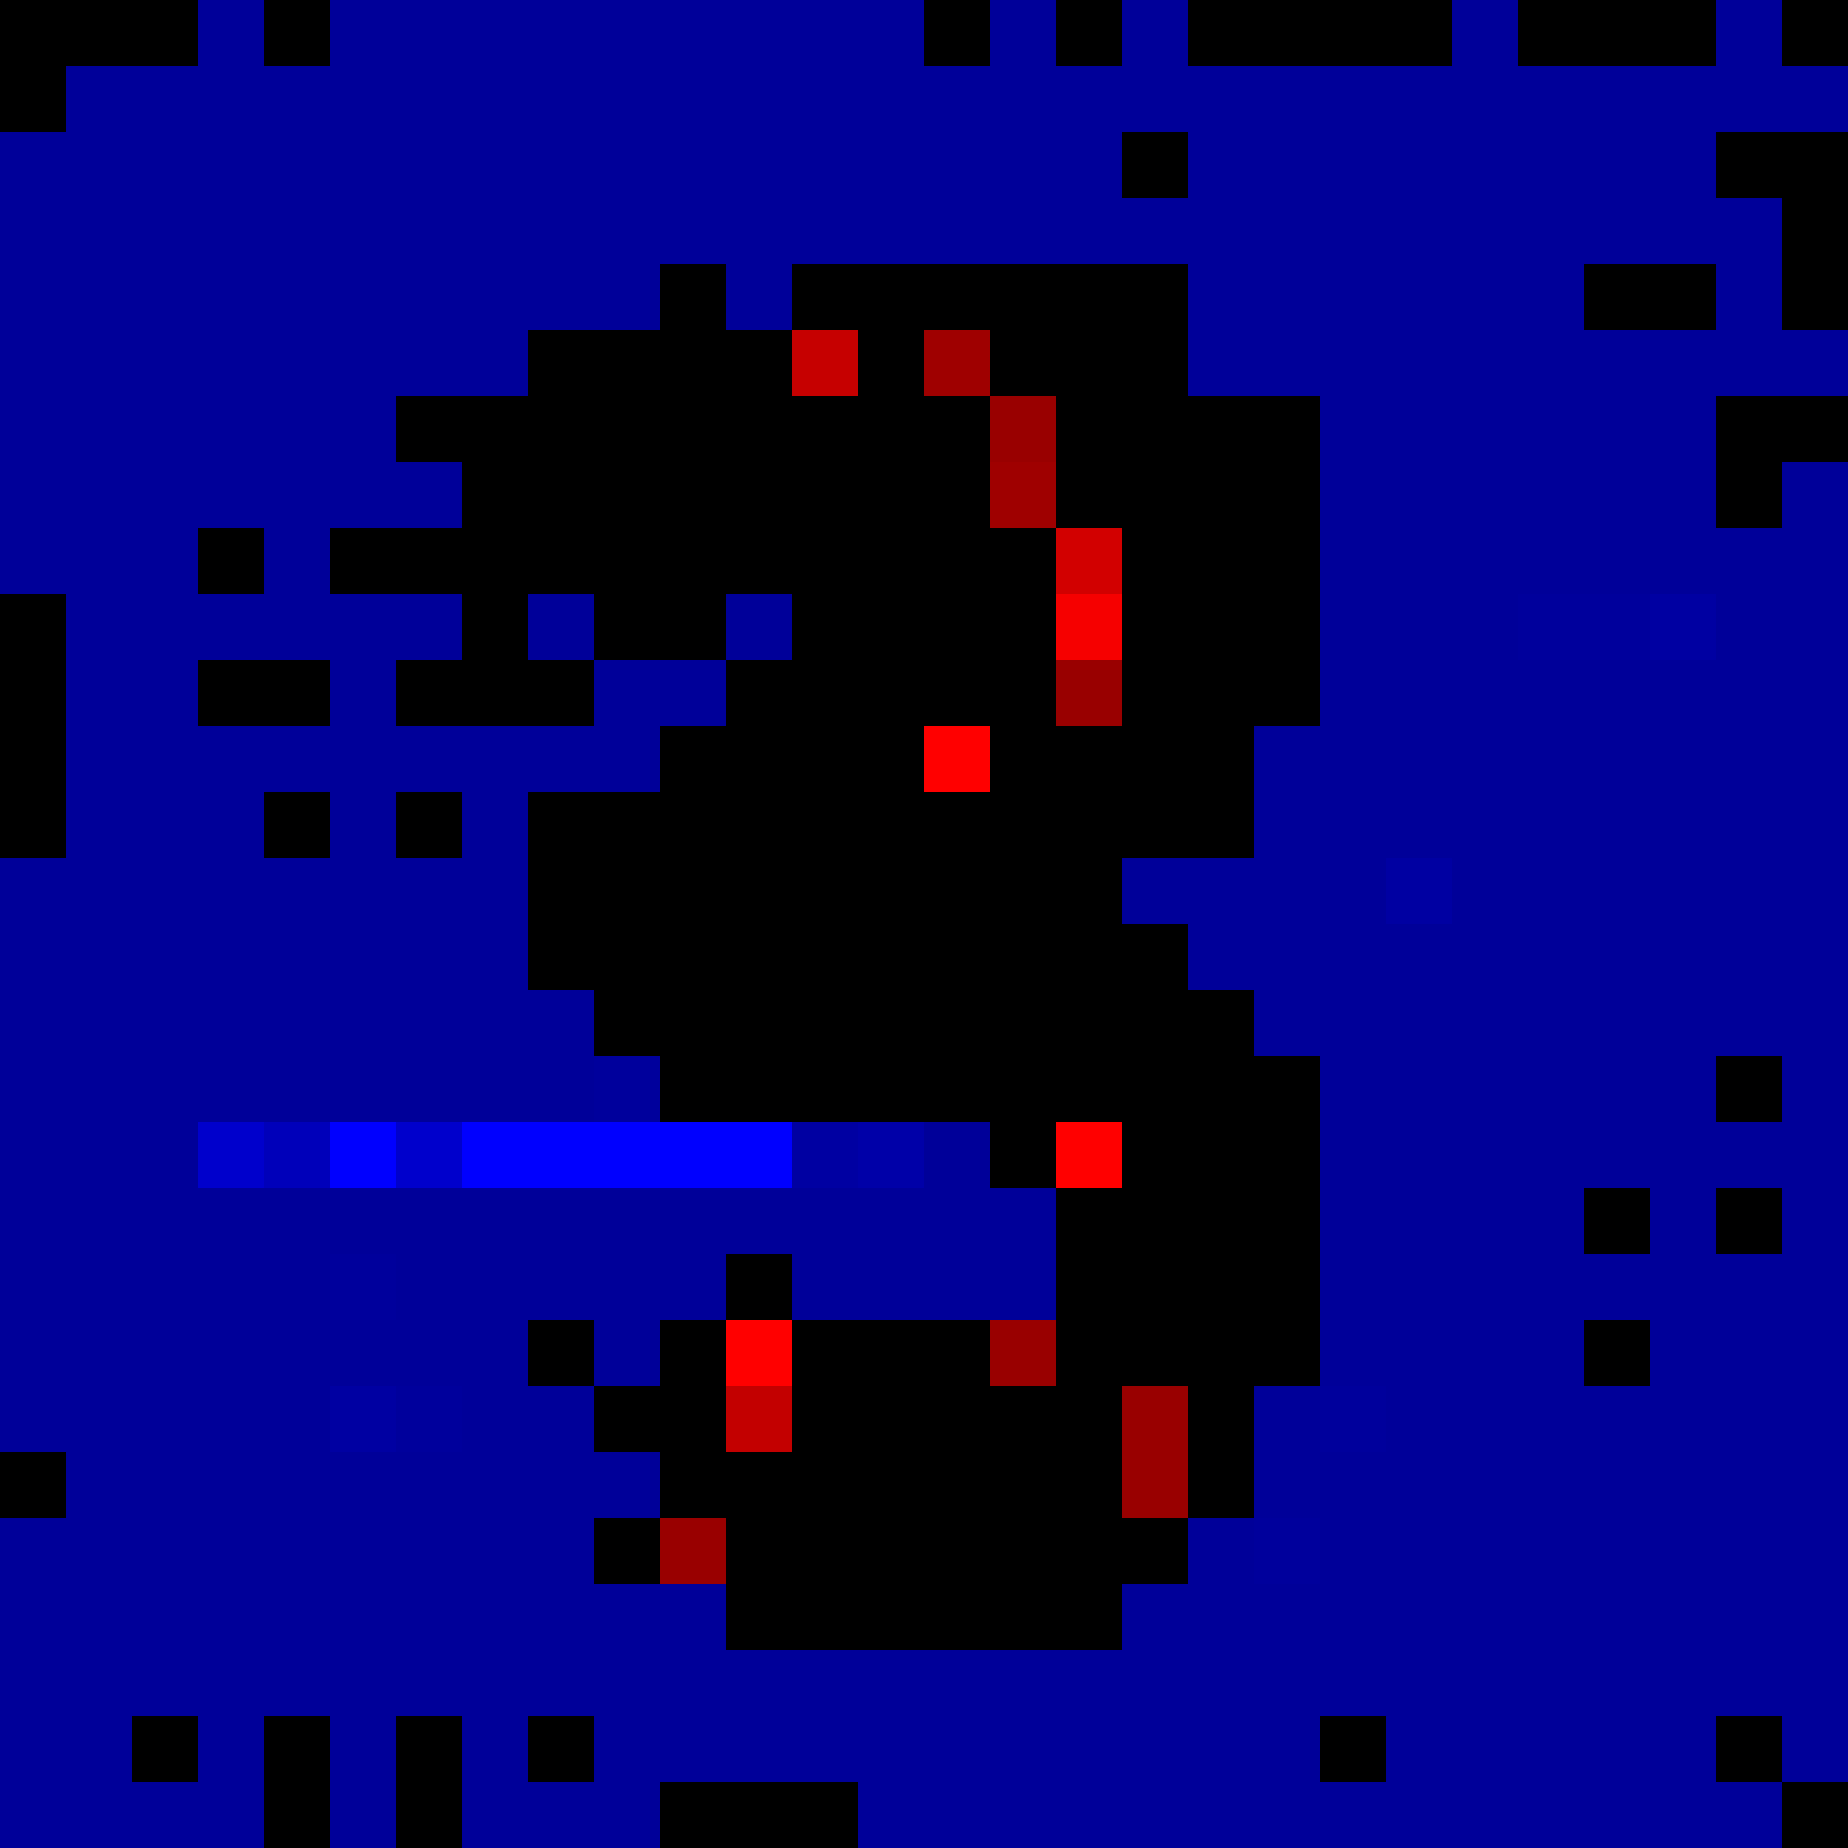
\includegraphics[width=\linewidth]{saliency/mnist_split_ic_saliency/image_036_true_3_pred_3/final_saliency_threshold_wrt_2_bright.png}\\[-1pt]{\scriptsize Logit 2}
		\end{minipage}%
		\begin{minipage}[b]{0.19\linewidth}\centering
			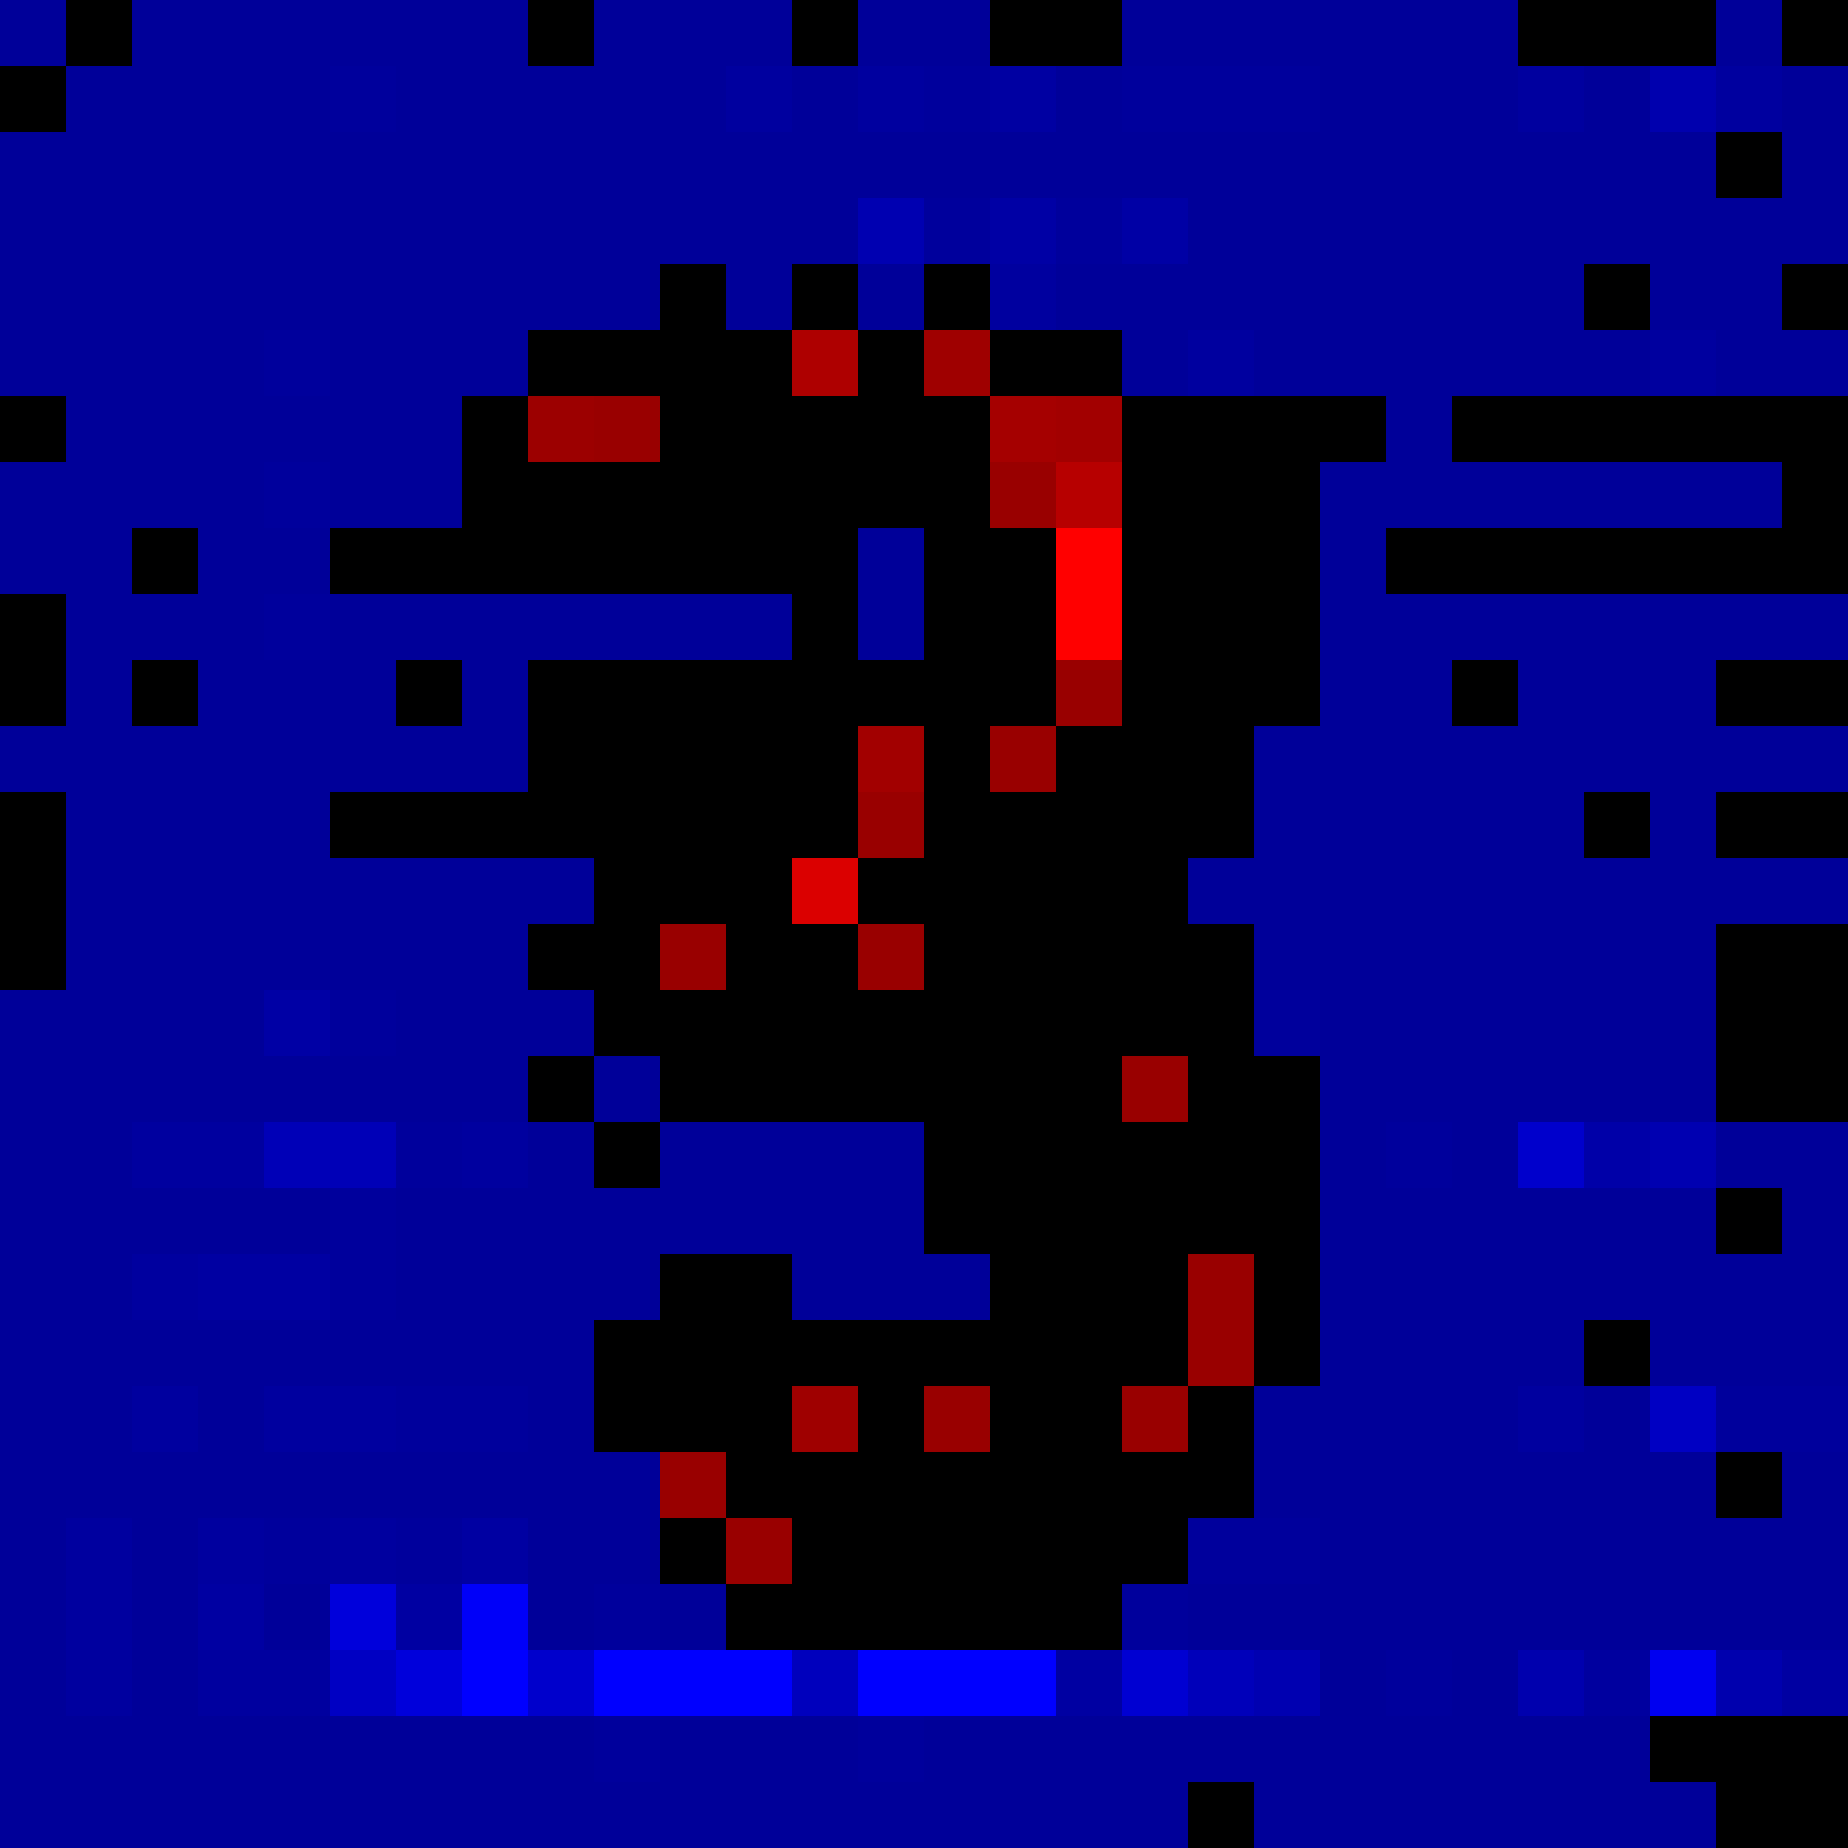
\includegraphics[width=\linewidth]{saliency/mnist_split_ic_saliency/image_036_true_3_pred_3/final_saliency_threshold_wrt_3_bright.png}\\[-1pt]{\scriptsize Logit 3}
		\end{minipage}%
		\begin{minipage}[b]{0.19\linewidth}\centering
			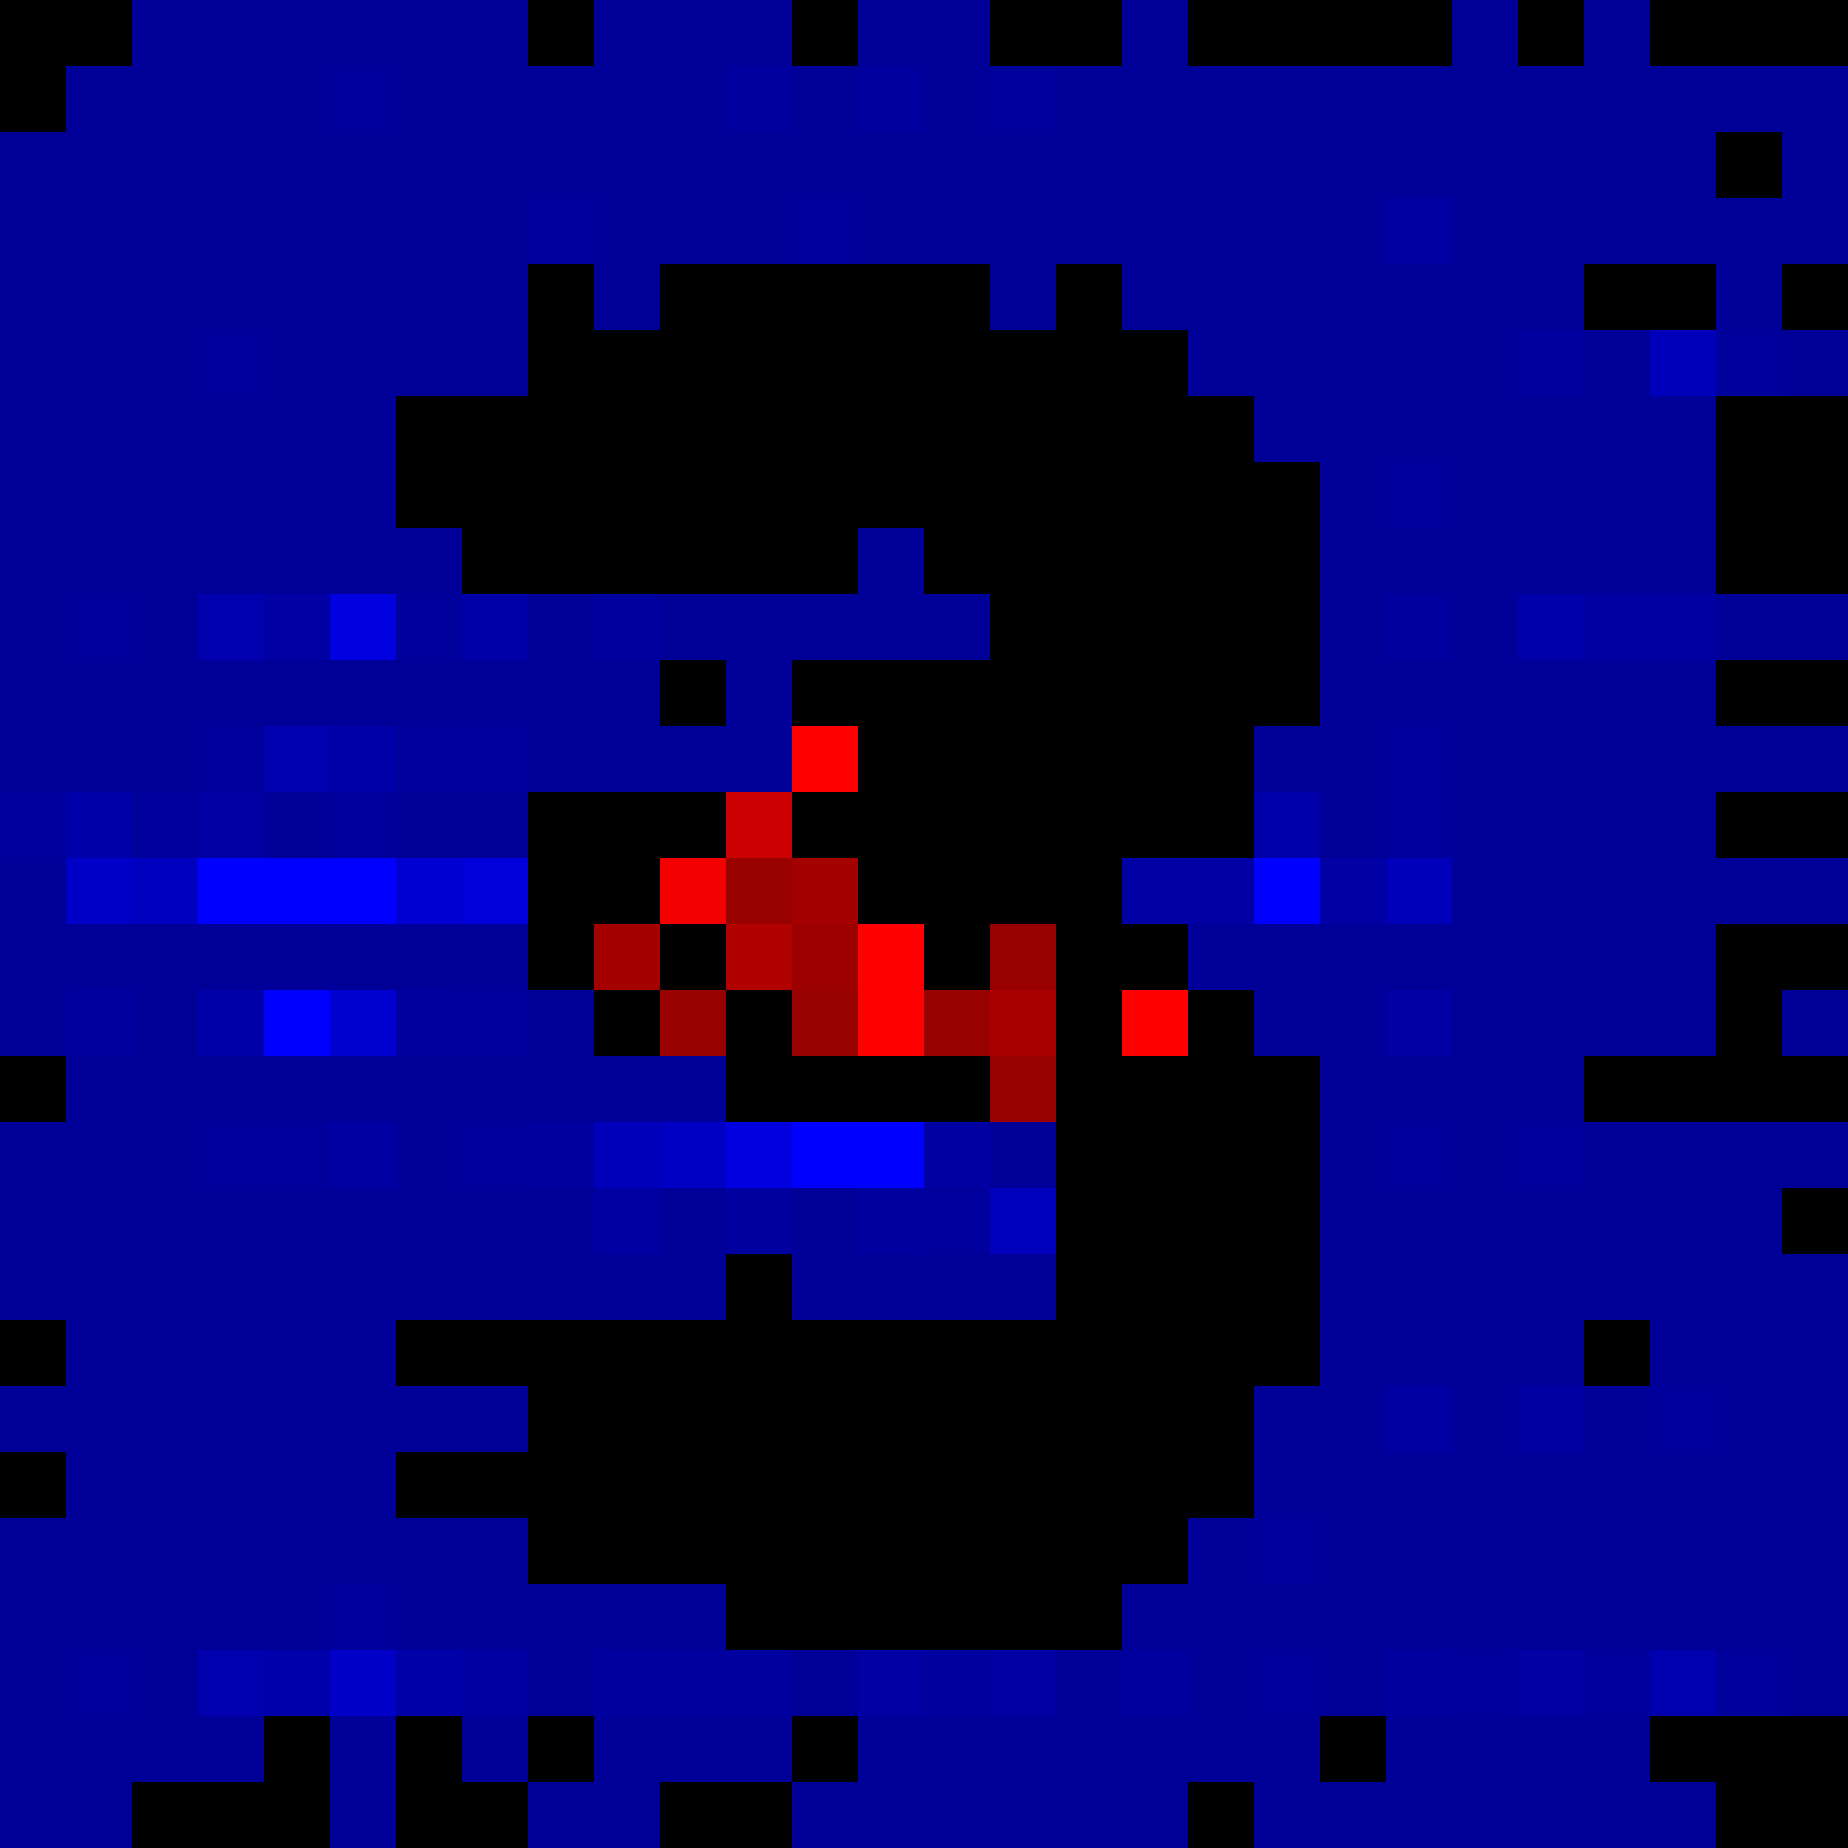
\includegraphics[width=\linewidth]{saliency/mnist_split_ic_saliency/image_036_true_3_pred_3/final_saliency_threshold_wrt_4_bright.png}\\[-1pt]{\scriptsize Logit 4}
		\end{minipage}

		\vspace{0.12cm}

		\begin{minipage}[b]{0.19\linewidth}\centering
			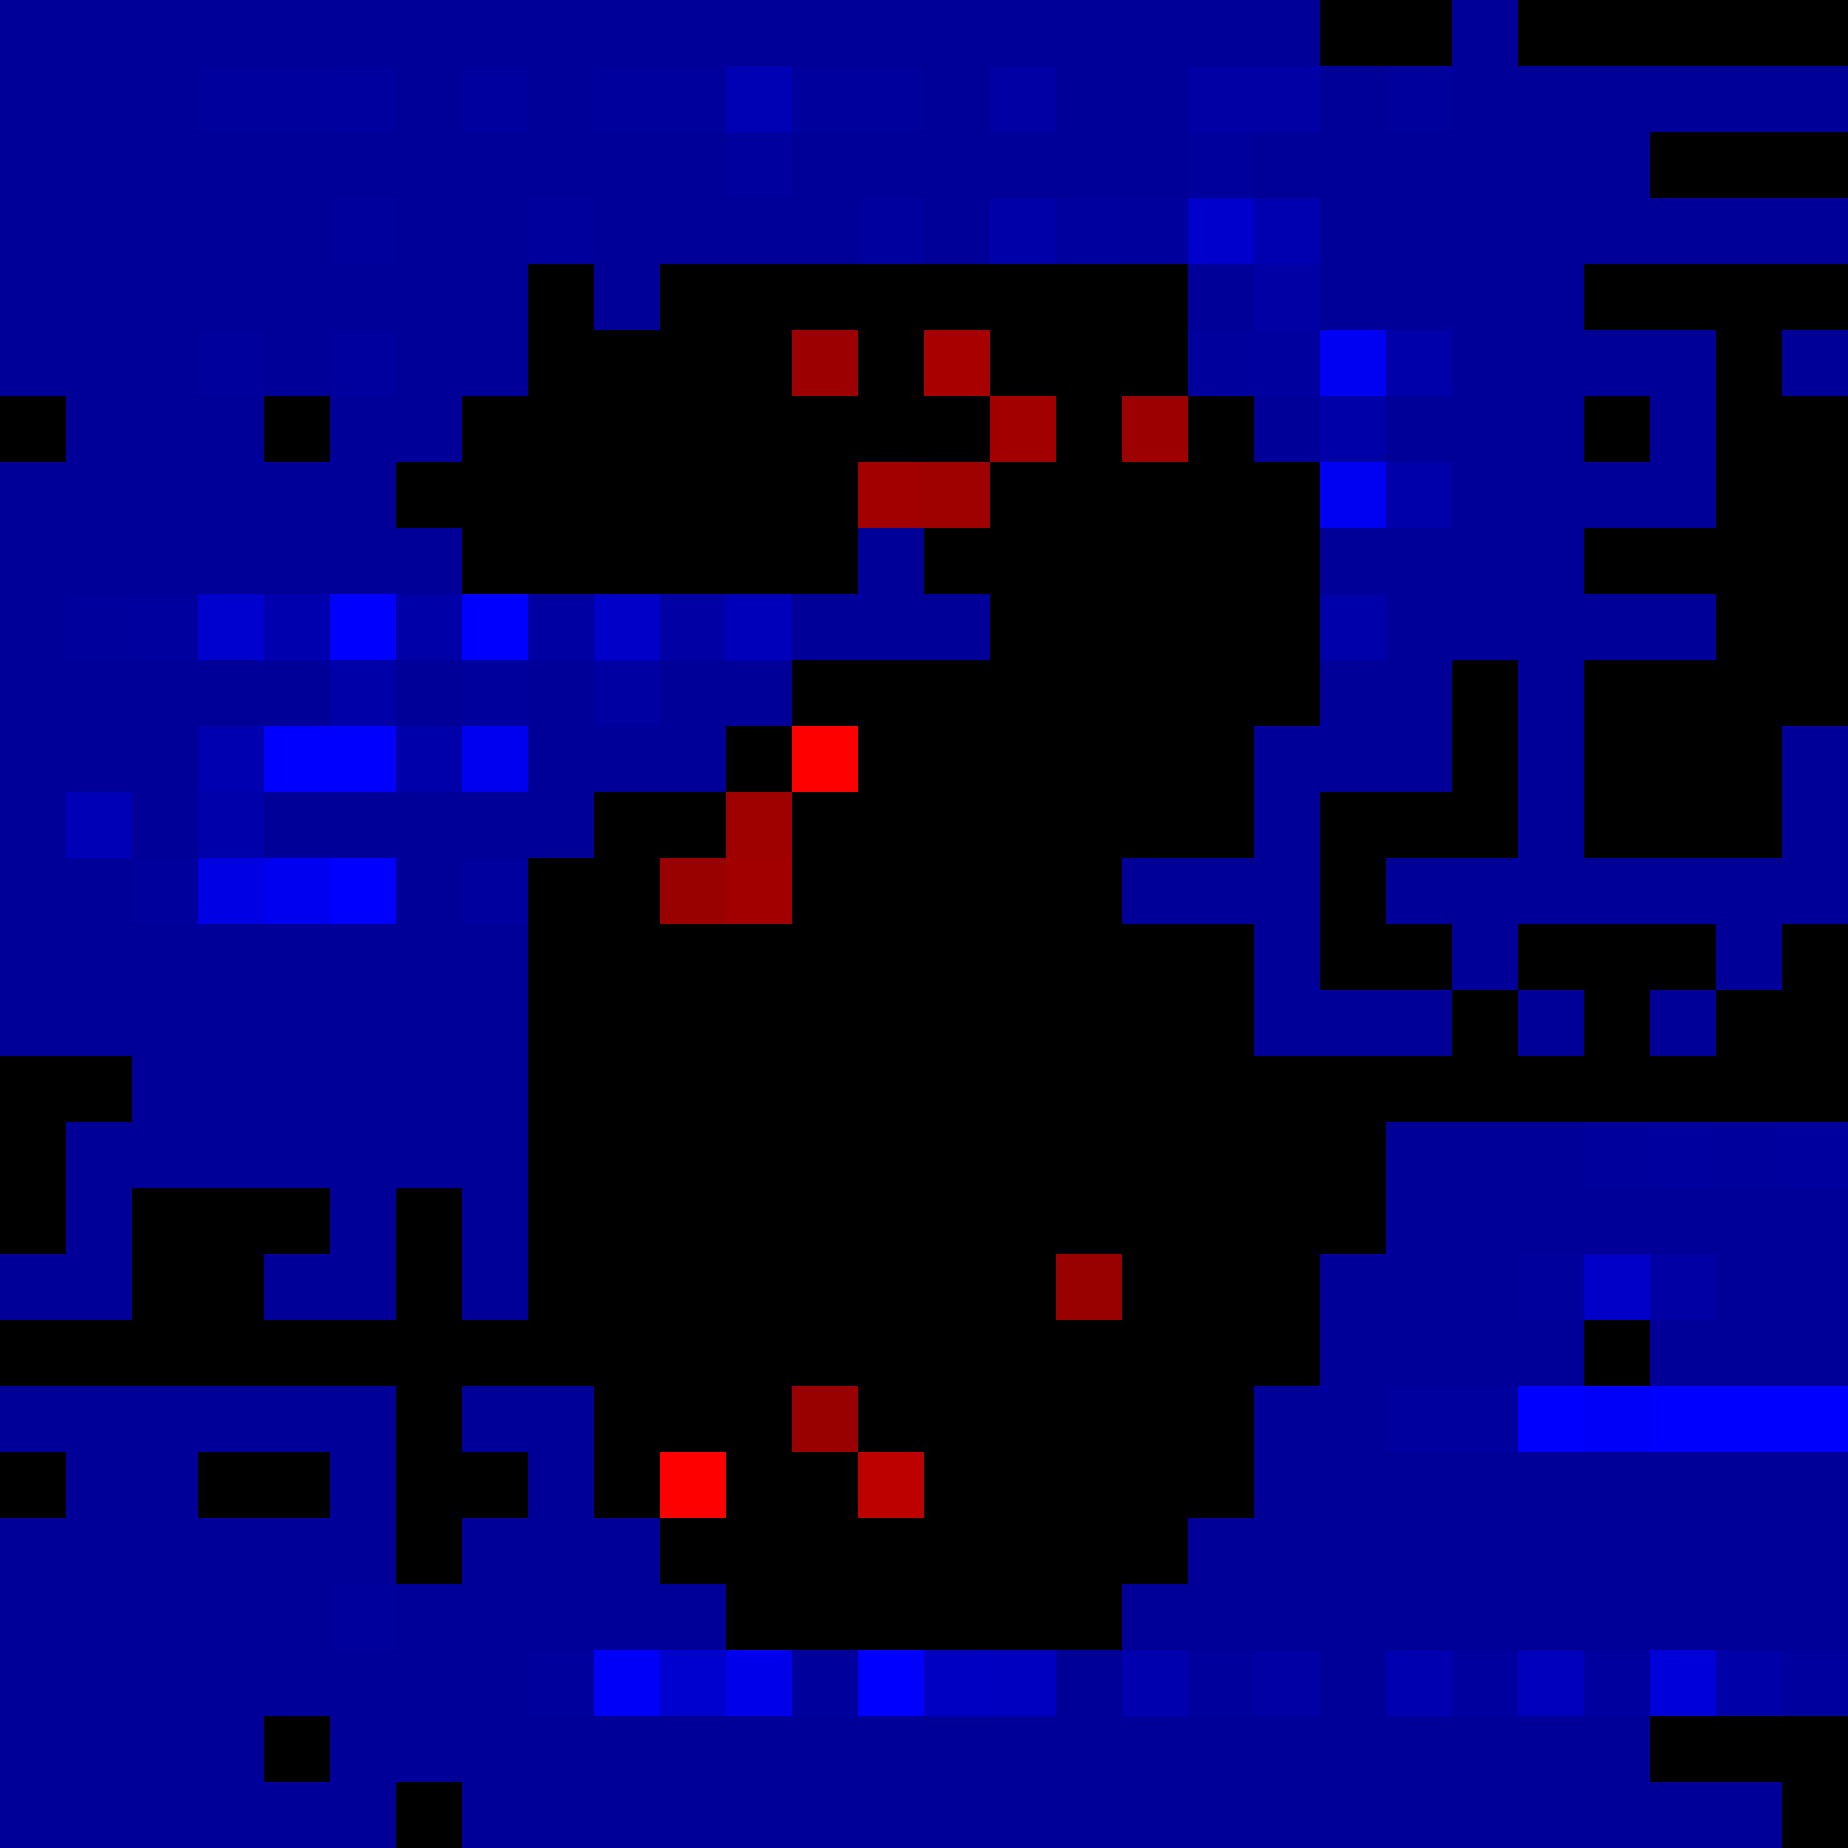
\includegraphics[width=\linewidth]{saliency/mnist_split_ic_saliency/image_036_true_3_pred_3/final_saliency_threshold_wrt_5_bright.png}\\[-1pt]{\scriptsize Logit 5}
		\end{minipage}%
		\begin{minipage}[b]{0.19\linewidth}\centering
			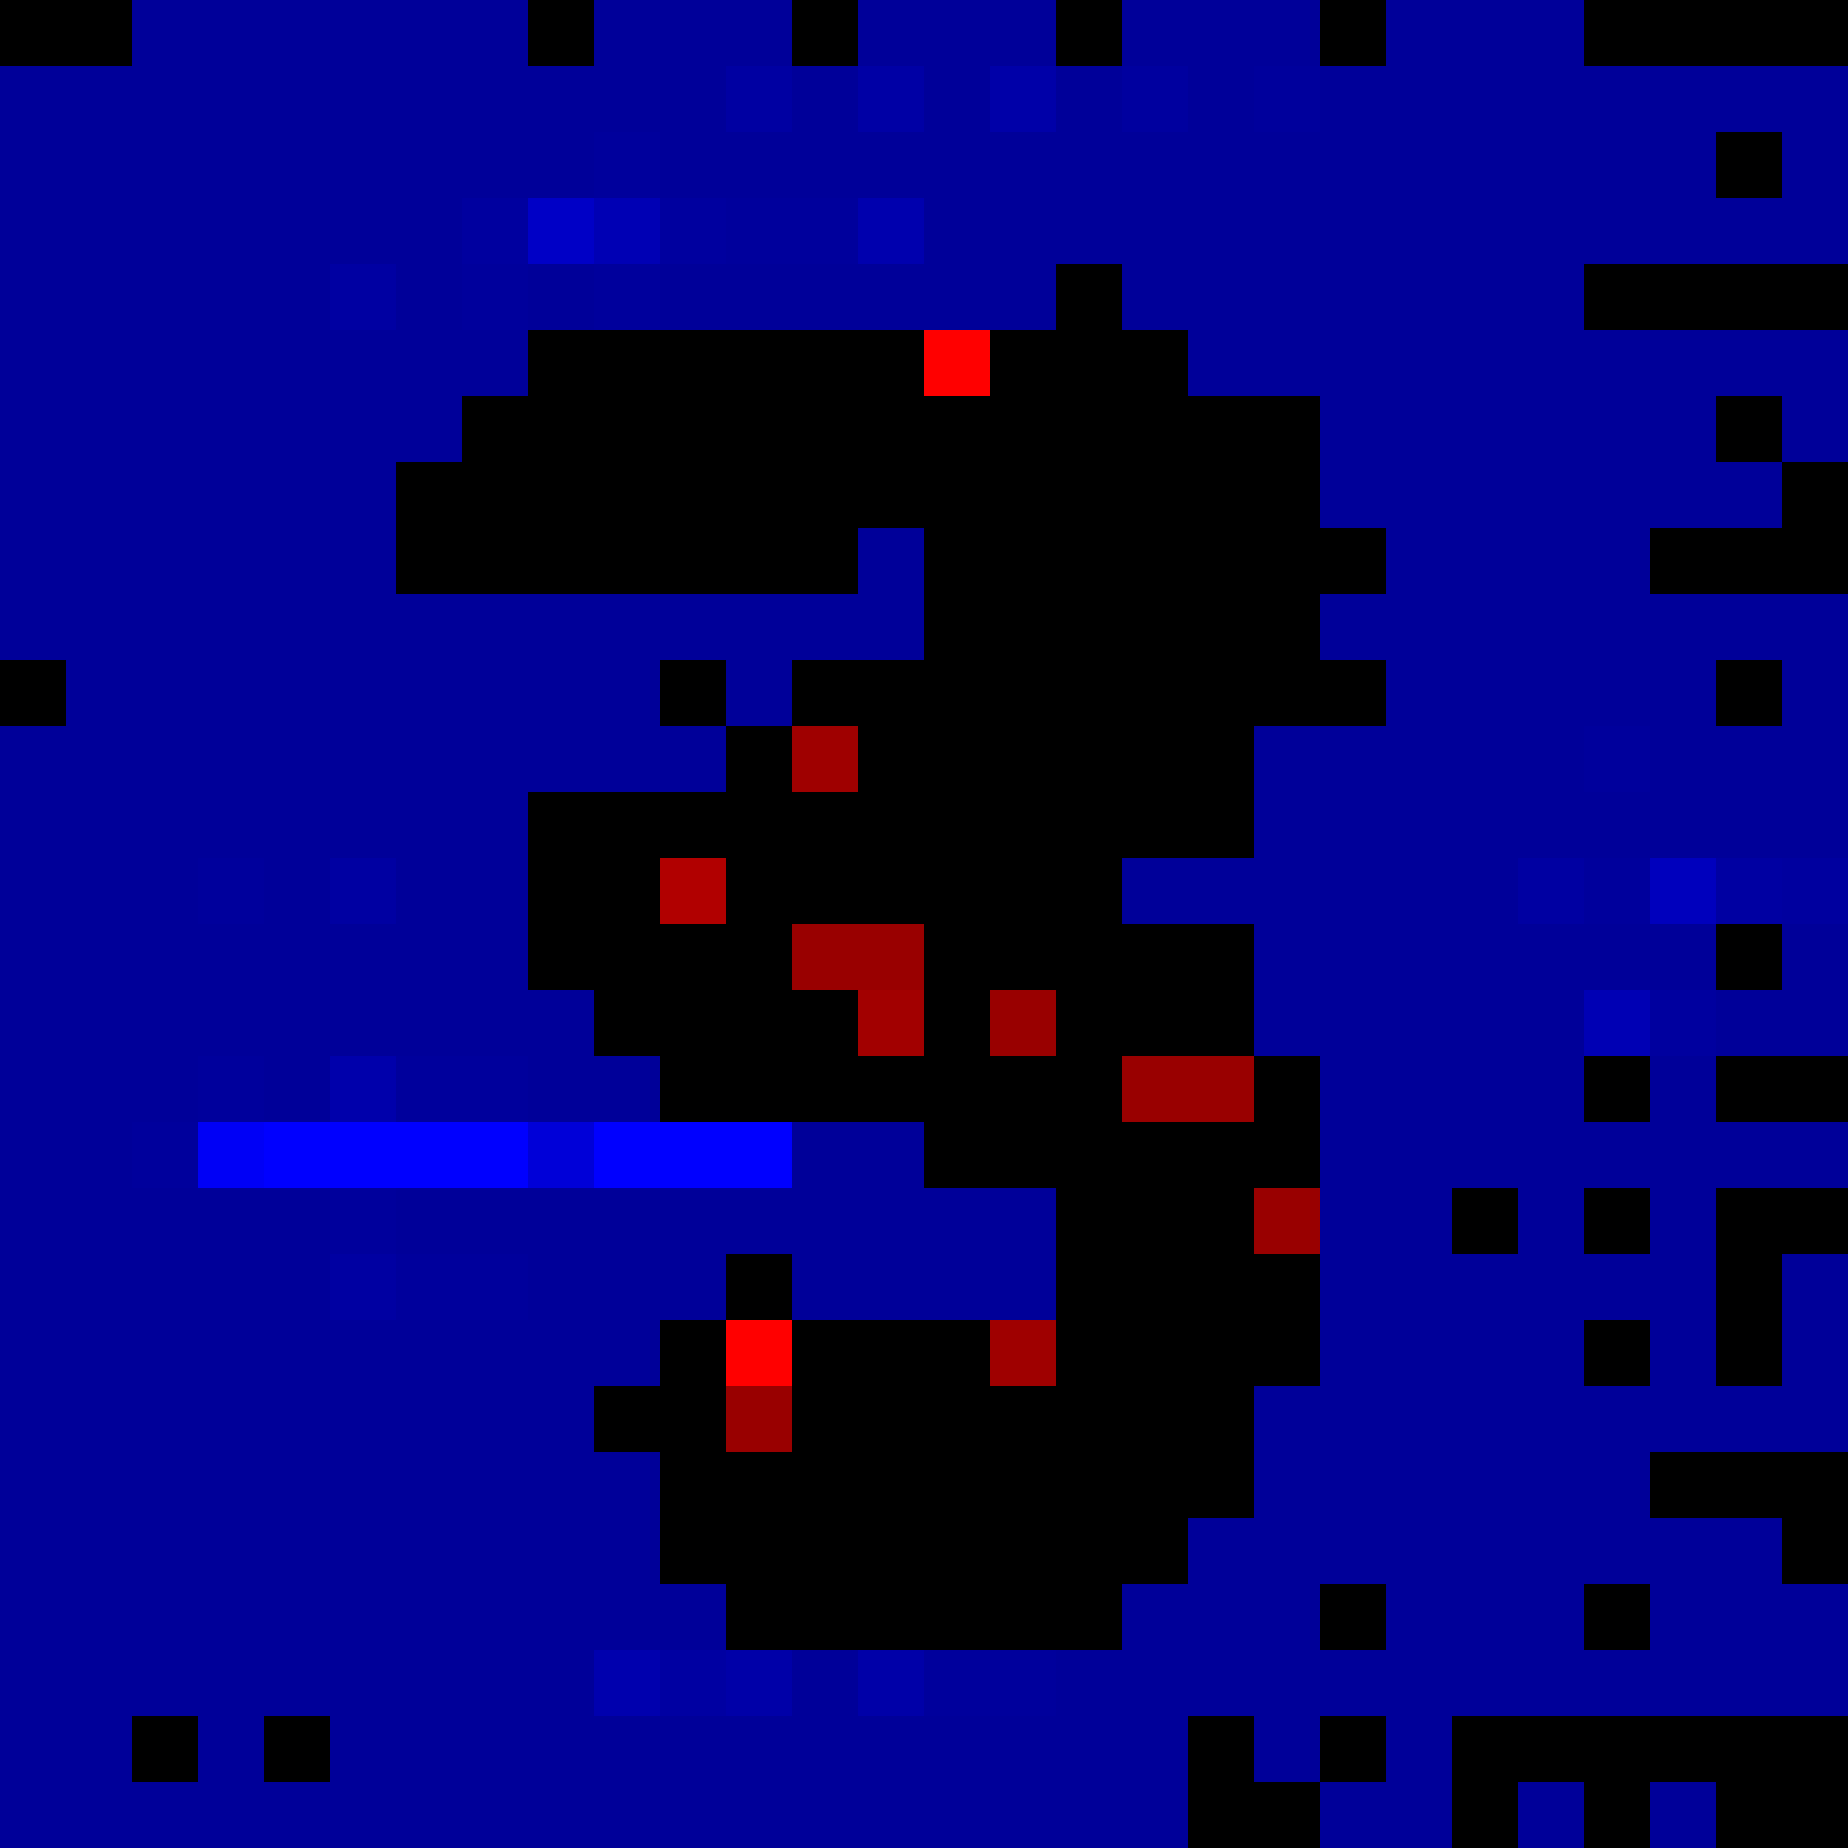
\includegraphics[width=\linewidth]{saliency/mnist_split_ic_saliency/image_036_true_3_pred_3/final_saliency_threshold_wrt_6_bright.png}\\[-1pt]{\scriptsize Logit 6}
		\end{minipage}%
		\begin{minipage}[b]{0.19\linewidth}\centering
			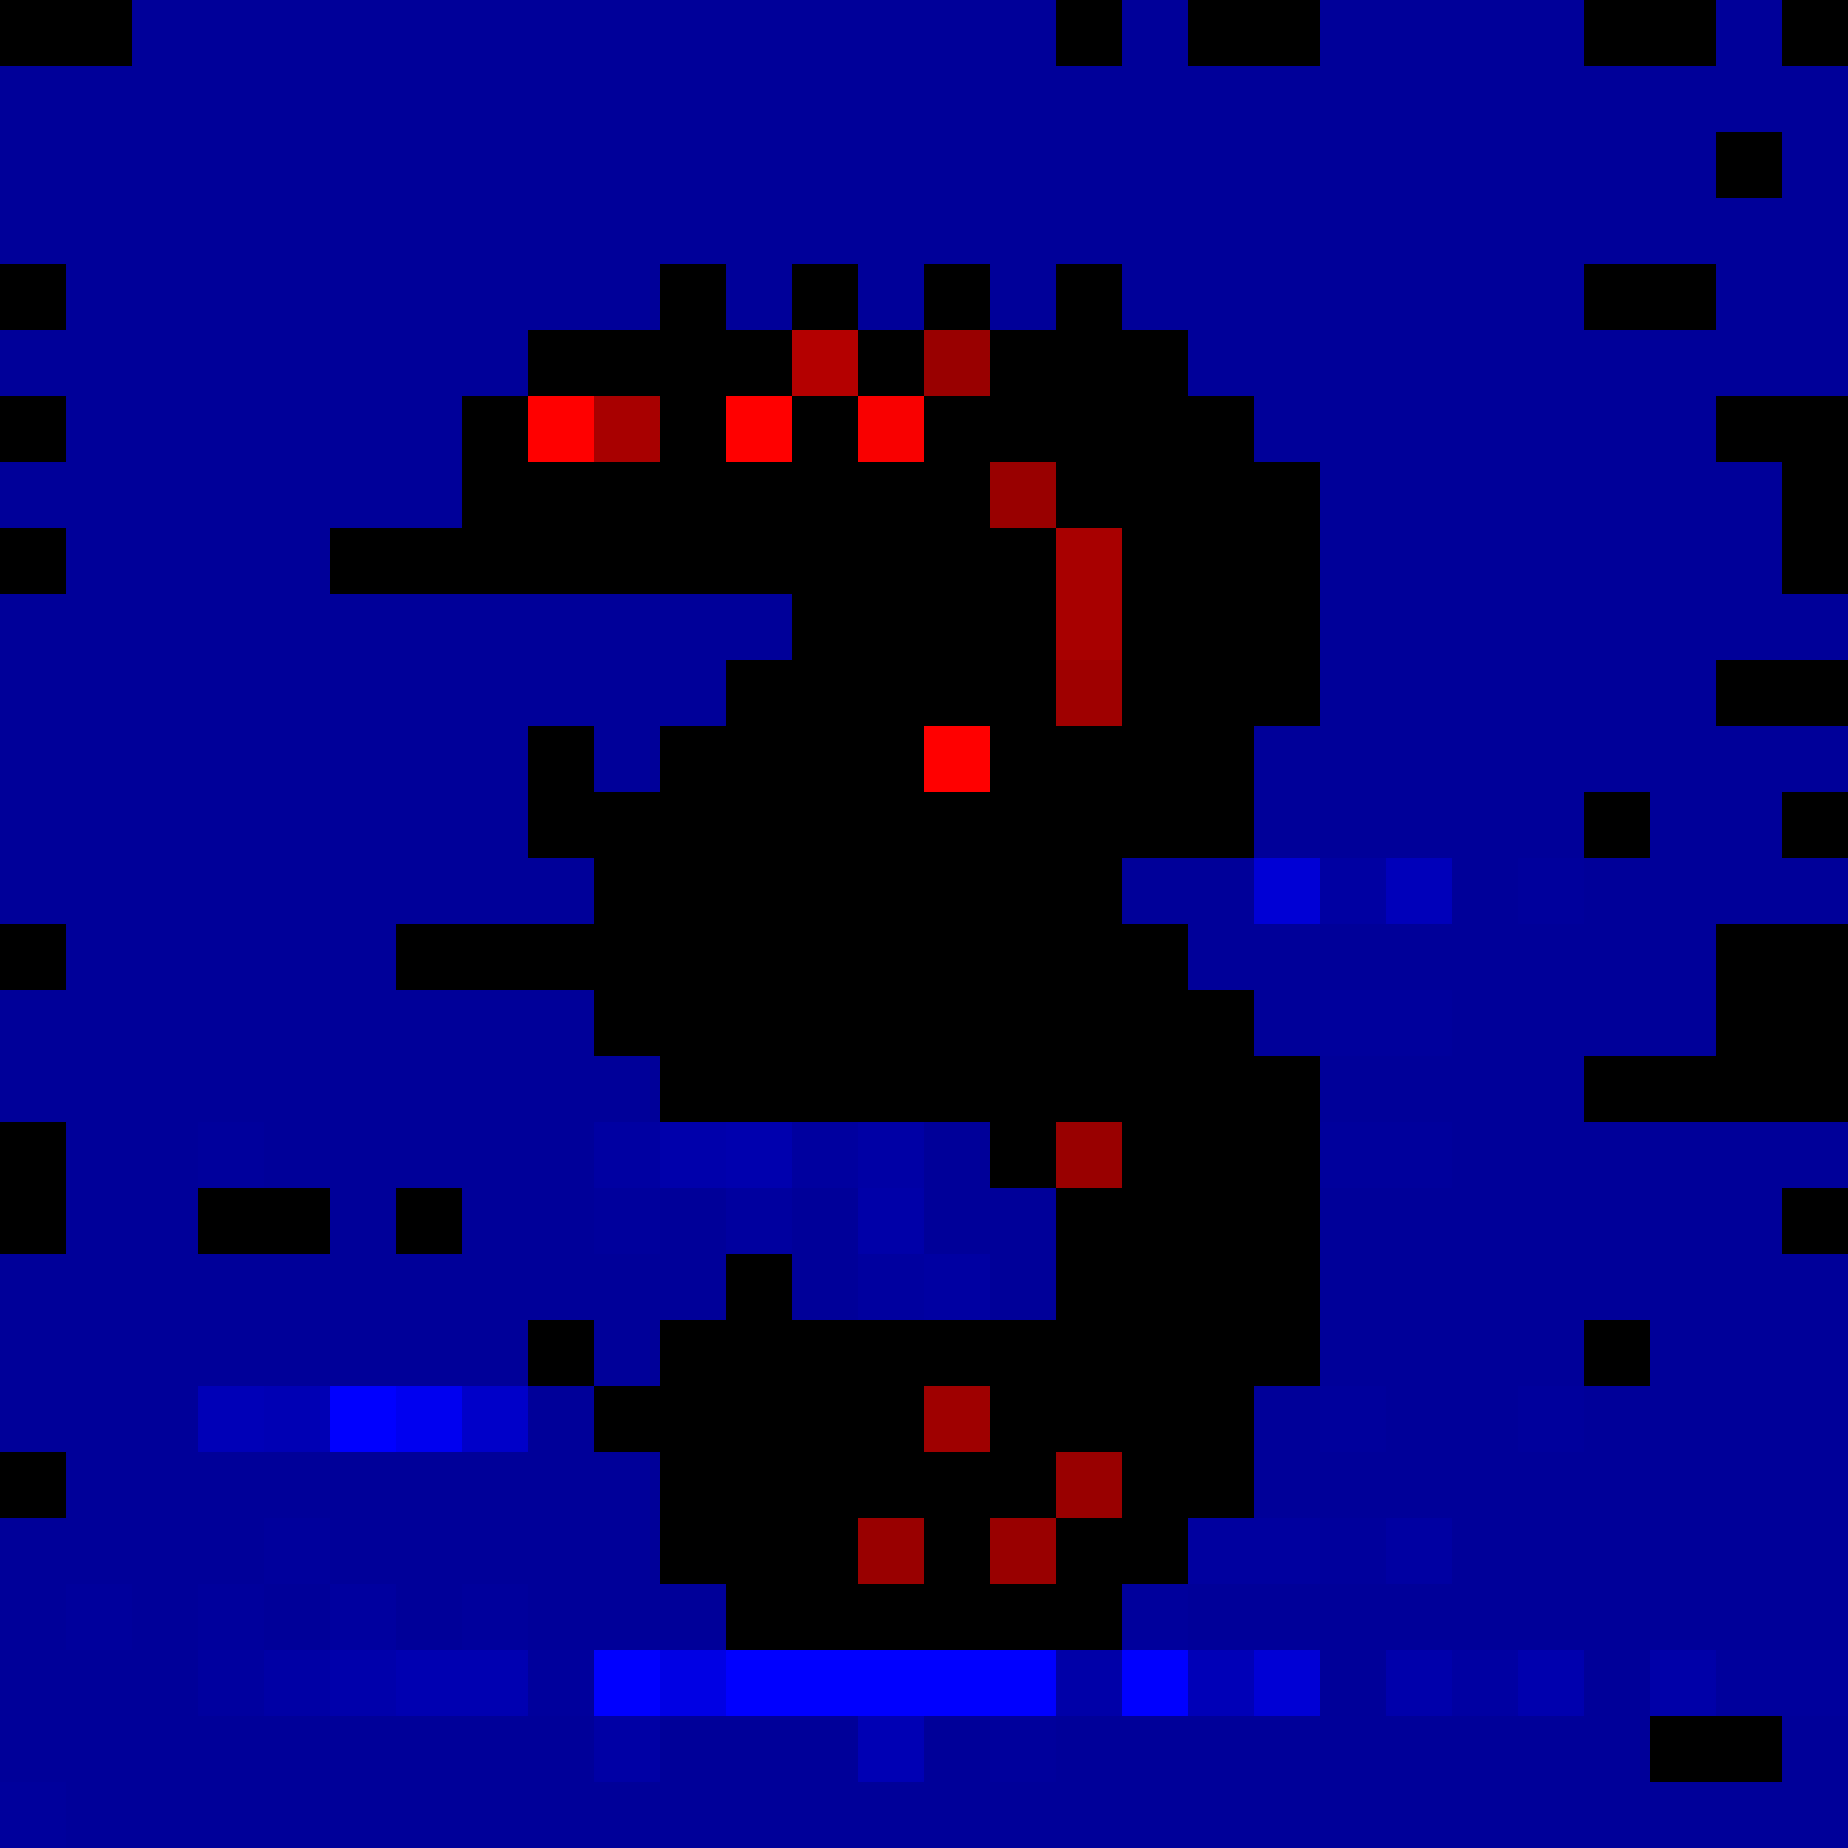
\includegraphics[width=\linewidth]{saliency/mnist_split_ic_saliency/image_036_true_3_pred_3/final_saliency_threshold_wrt_7_bright.png}\\[-1pt]{\scriptsize Logit 7}
		\end{minipage}%
		\begin{minipage}[b]{0.19\linewidth}\centering
			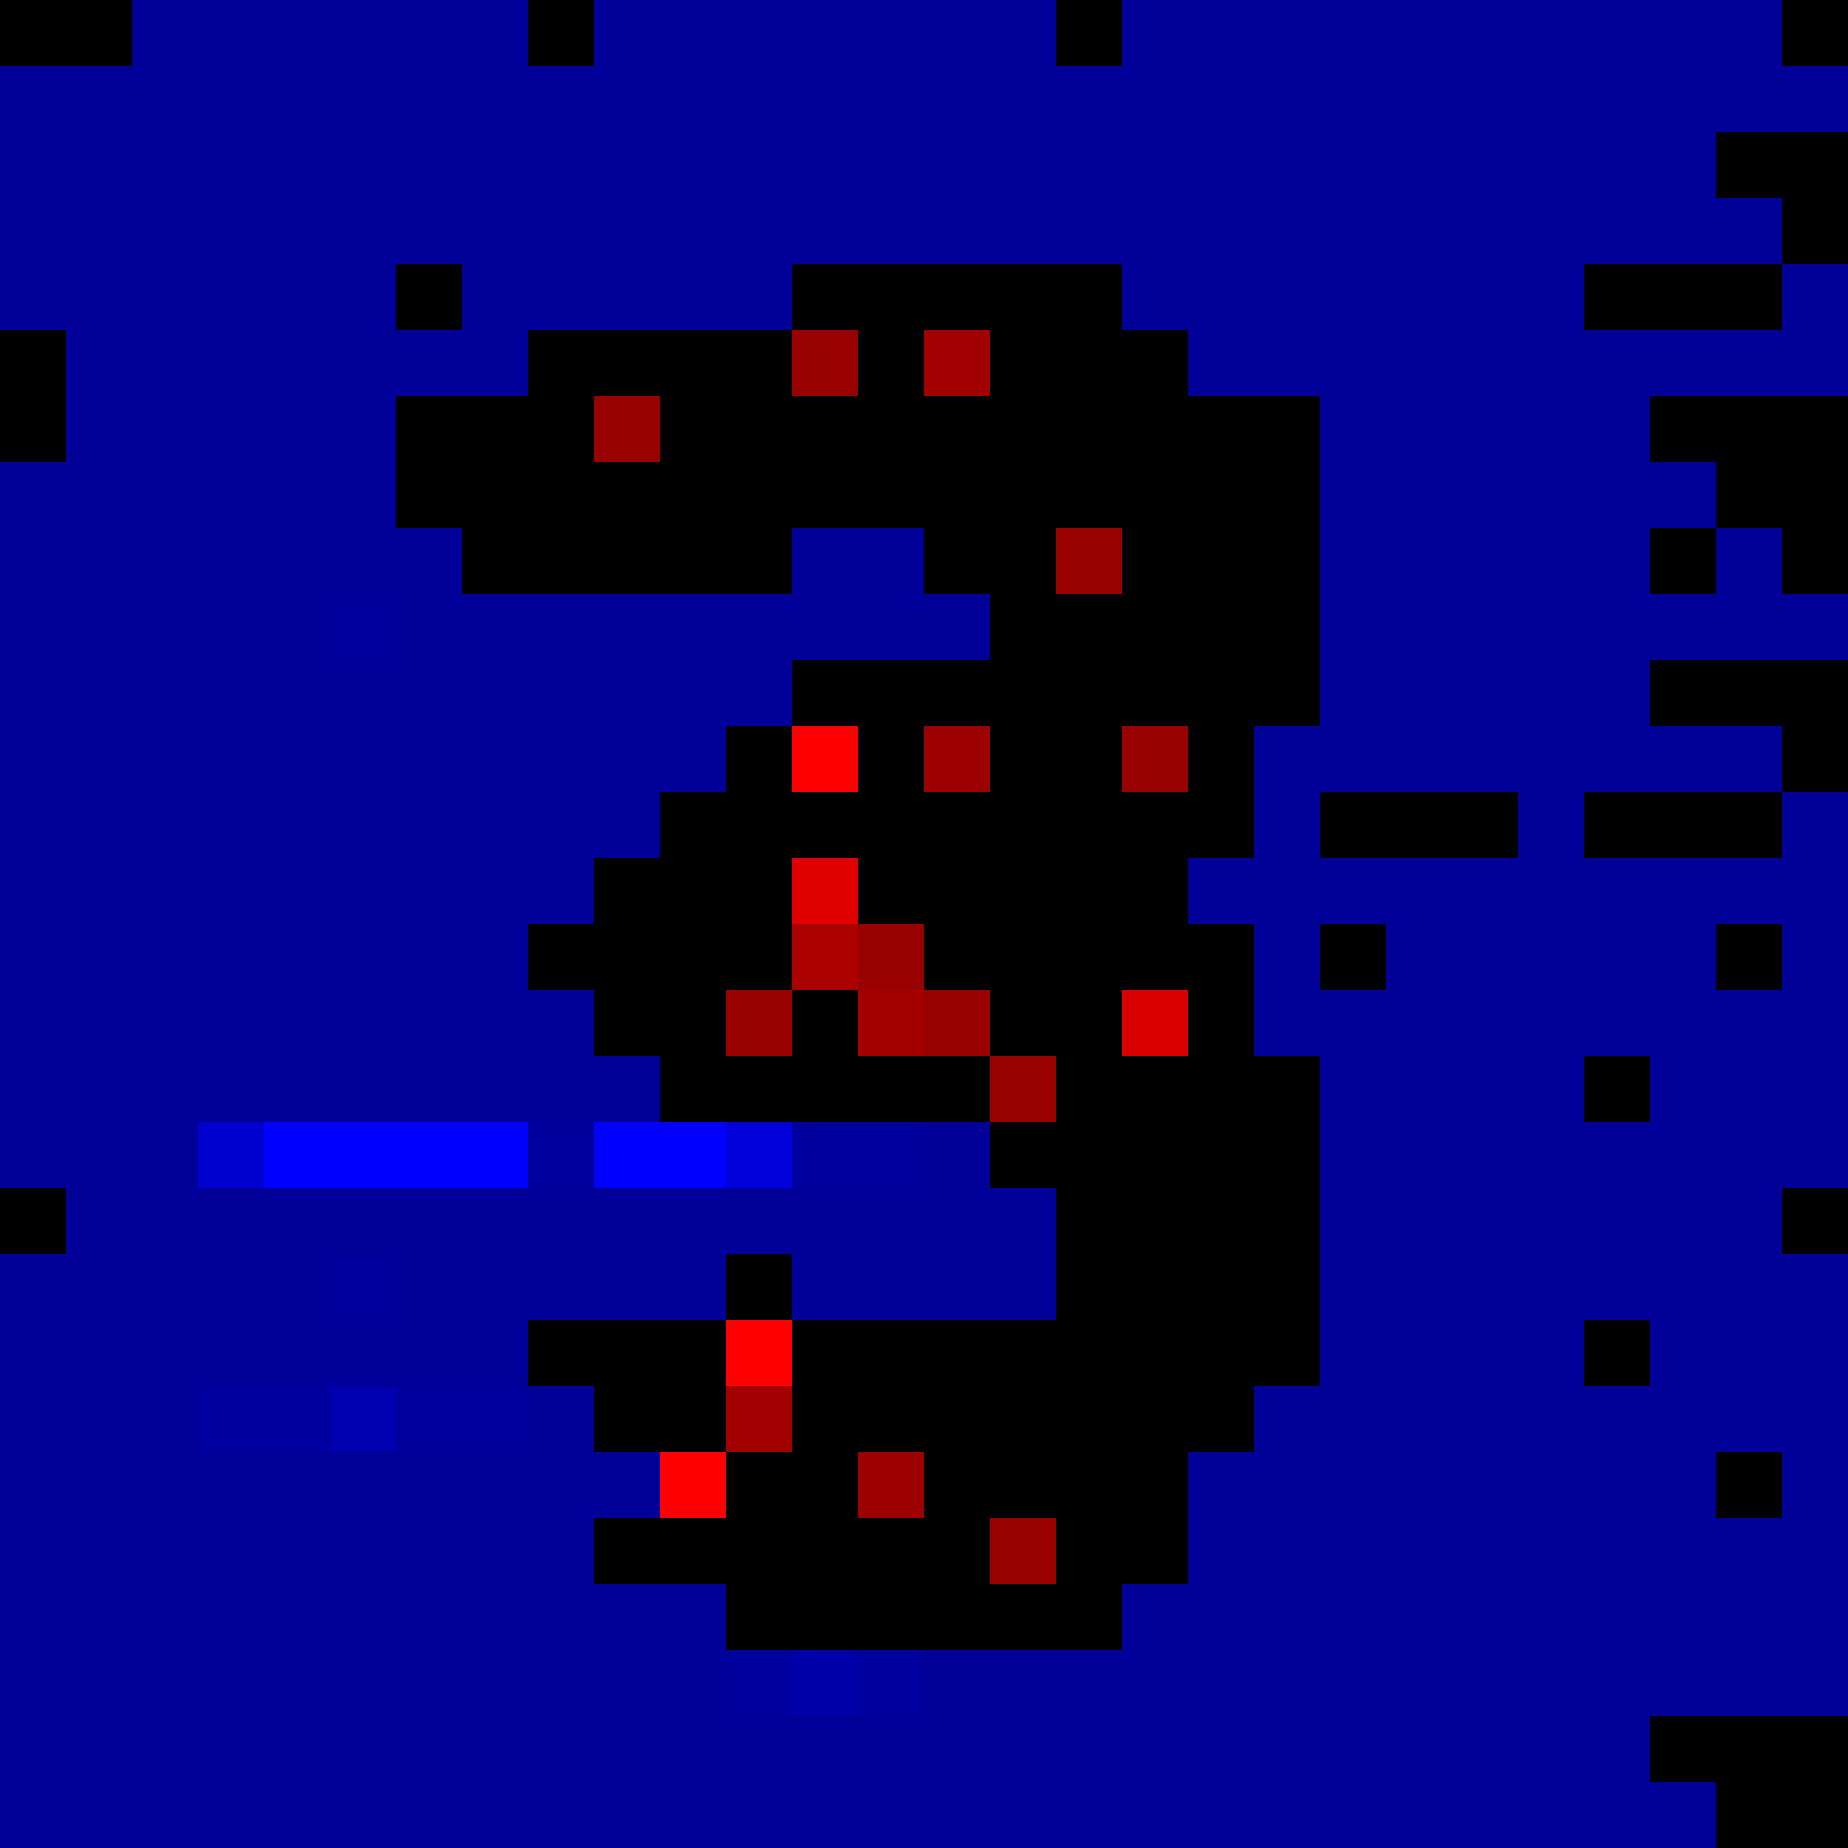
\includegraphics[width=\linewidth]{saliency/mnist_split_ic_saliency/image_036_true_3_pred_3/final_saliency_threshold_wrt_8_bright.png}\\[-1pt]{\scriptsize Logit 8}
		\end{minipage}%
		\begin{minipage}[b]{0.19\linewidth}\centering
			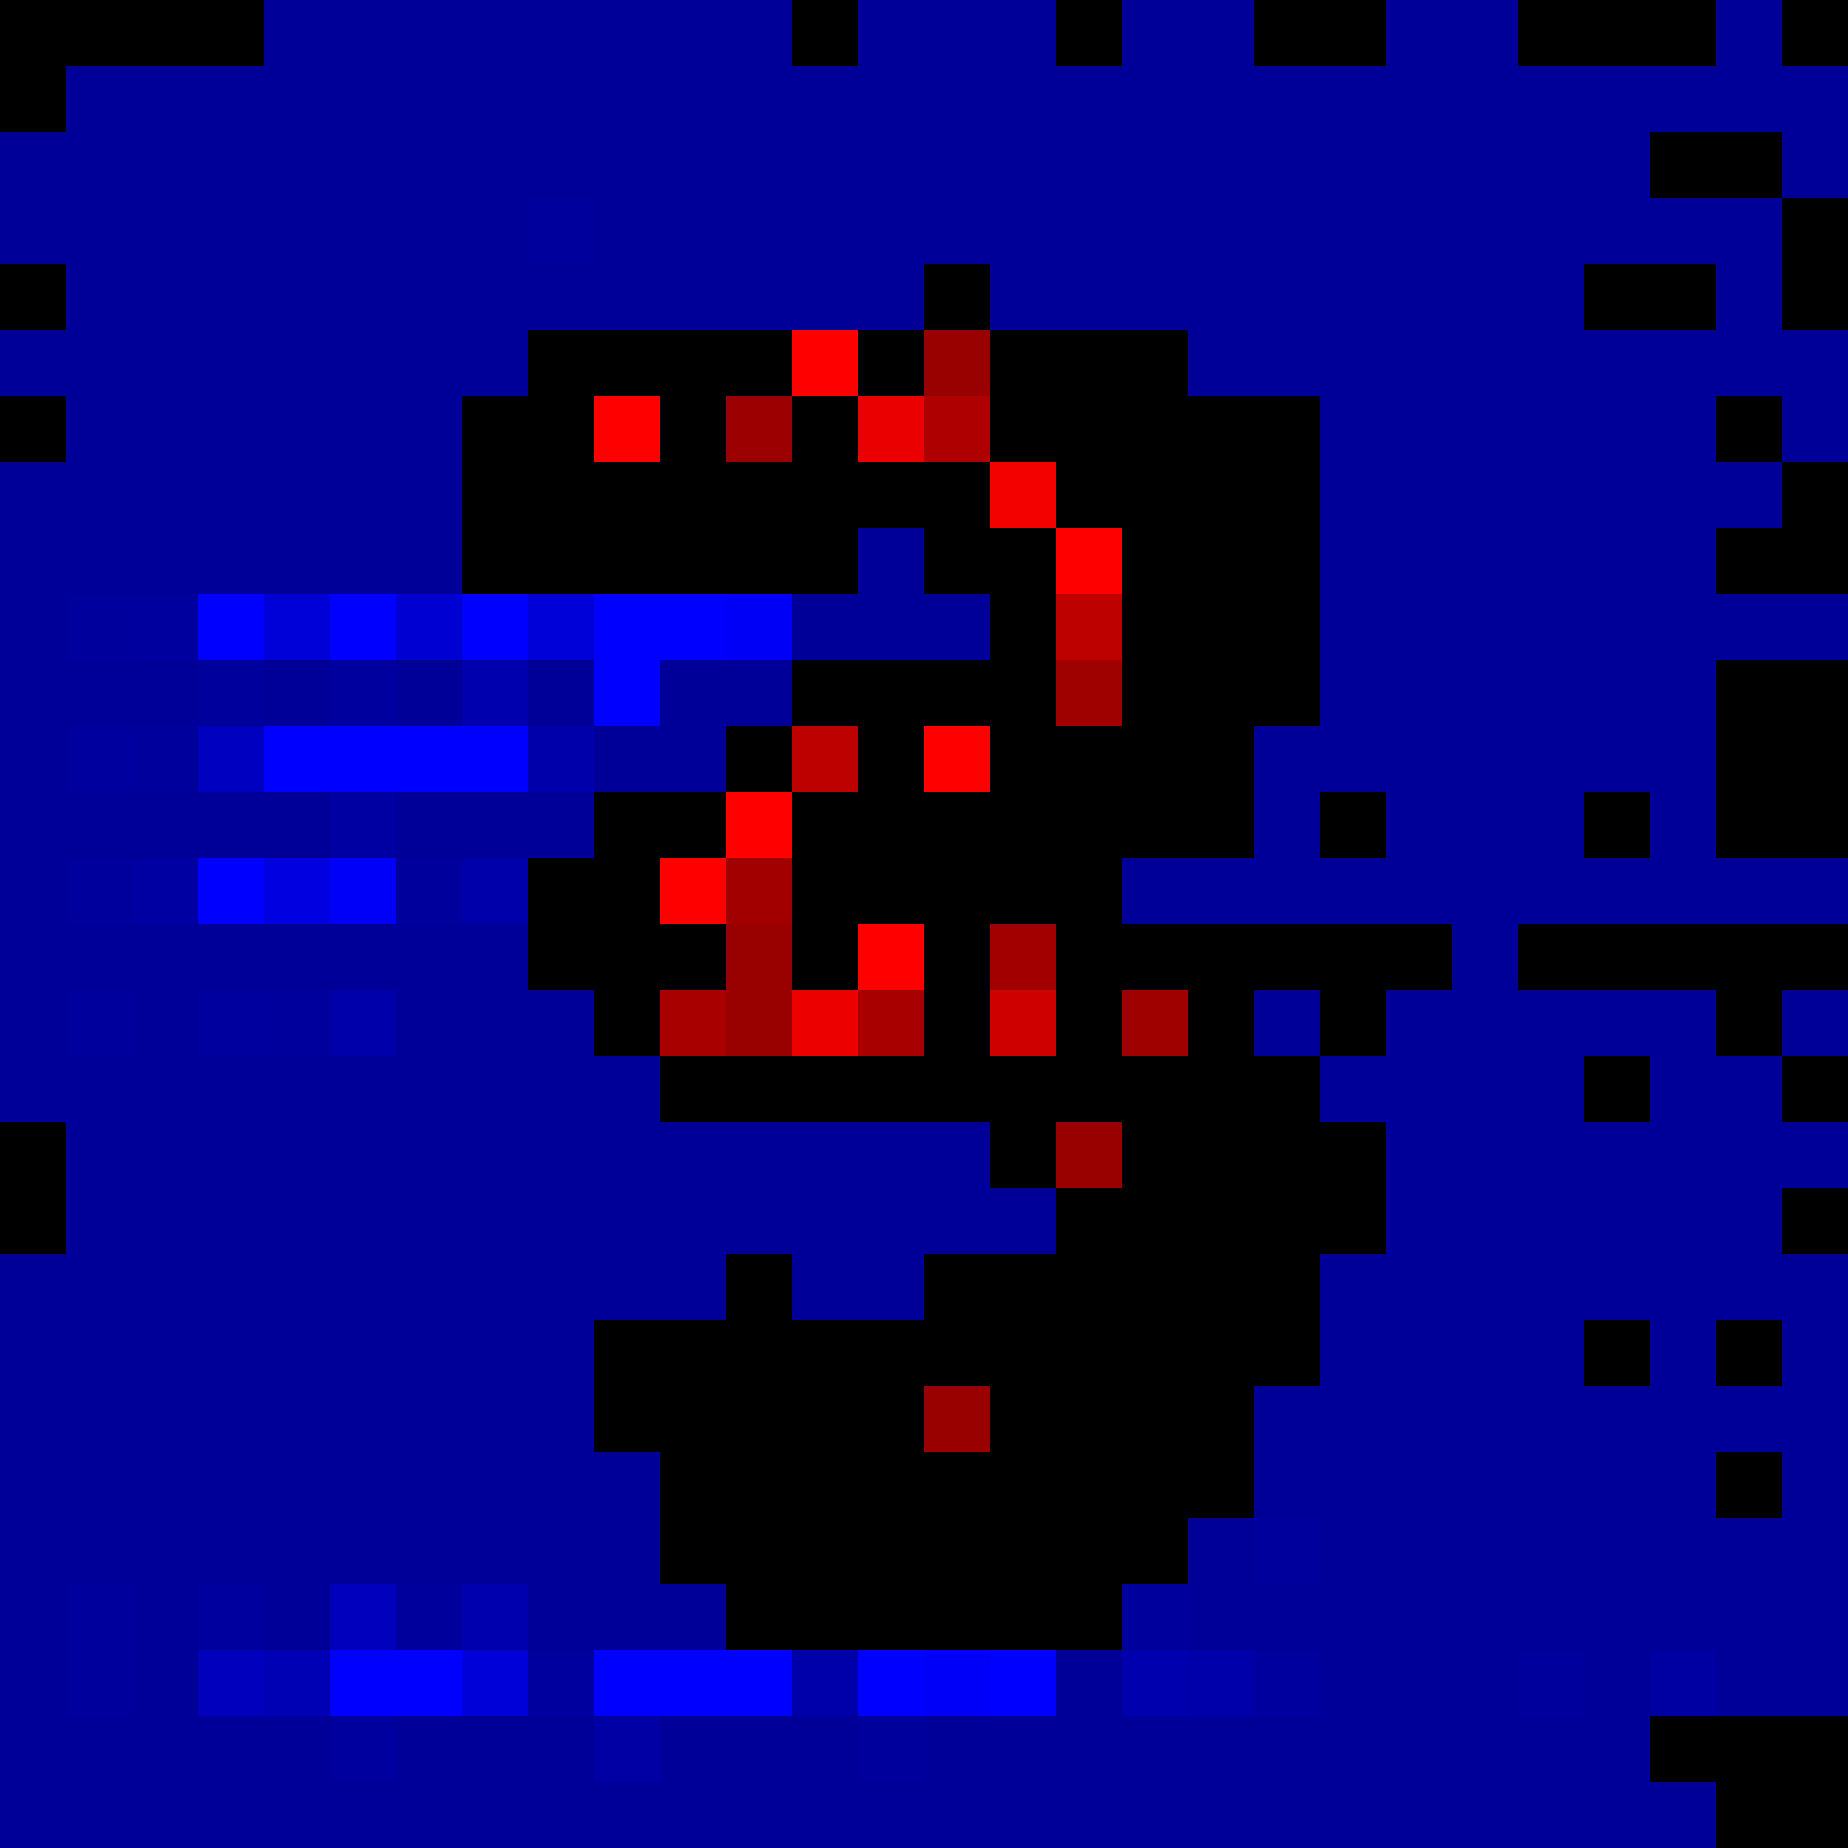
\includegraphics[width=\linewidth]{saliency/mnist_split_ic_saliency/image_036_true_3_pred_3/final_saliency_threshold_wrt_9_bright.png}\\[-1pt]{\scriptsize Logit 9}
		\end{minipage}
	\end{minipage}
	}%
\caption[Second example of inverted-input DIC stream gradients]{Second correctly classified MNIST test ``3'', using the model, per-class thresholded overlays and color convention of Figure~\ref{fig:mnist_split_ic_saliency}. Left: input. These stream-local maps do not by themselves establish the effect of adding pixels on the complete model.}
	\label{fig:mnist_split_ic_saliency_second}
\end{figure}

Figure~\ref{fig:mnist_split_ic_saliency} overlays both gradients for each class logit of a test ``3''. The $g$-gradient best traces strokes for the ground-truth logit; for competing ``6'', ``8'' and ``9'', $h$-gradients concentrate \emph{between the arches}, where added pixels would geometrically close loops. A second correctly classified ``3'' (Figure~\ref{fig:mnist_split_ic_saliency_second}) shows the same qualitative pattern. The single \texttt{cnn\_maxout} IC model's gradients are mostly positive on strokes and negative on background, with less class-dependent directional variation. These examples suggest a role for the difference structure without establishing general disentanglement.

\paragraph{Qualitative comparison with a single input-convex model.}
Figure~\ref{fig:mnist_ic_saliency} reproduces the source paper's ten-class input-gradient comparison for the single \texttt{cnn\_maxout} IC model, showing the stroke/background sign pattern described above. Together with the class-dependent DICIN maps (Figures~\ref{fig:mnist_split_ic_saliency},~\ref{fig:mnist_split_ic_saliency_second}), it motivates a factual/counterfactual reading; finite-intervention effects and separation across all inputs and models require further tests.

\begin{figure}[t]
\QualitativeImageContent{
    \centering
    \begin{minipage}[b]{0.09\linewidth}\centering
        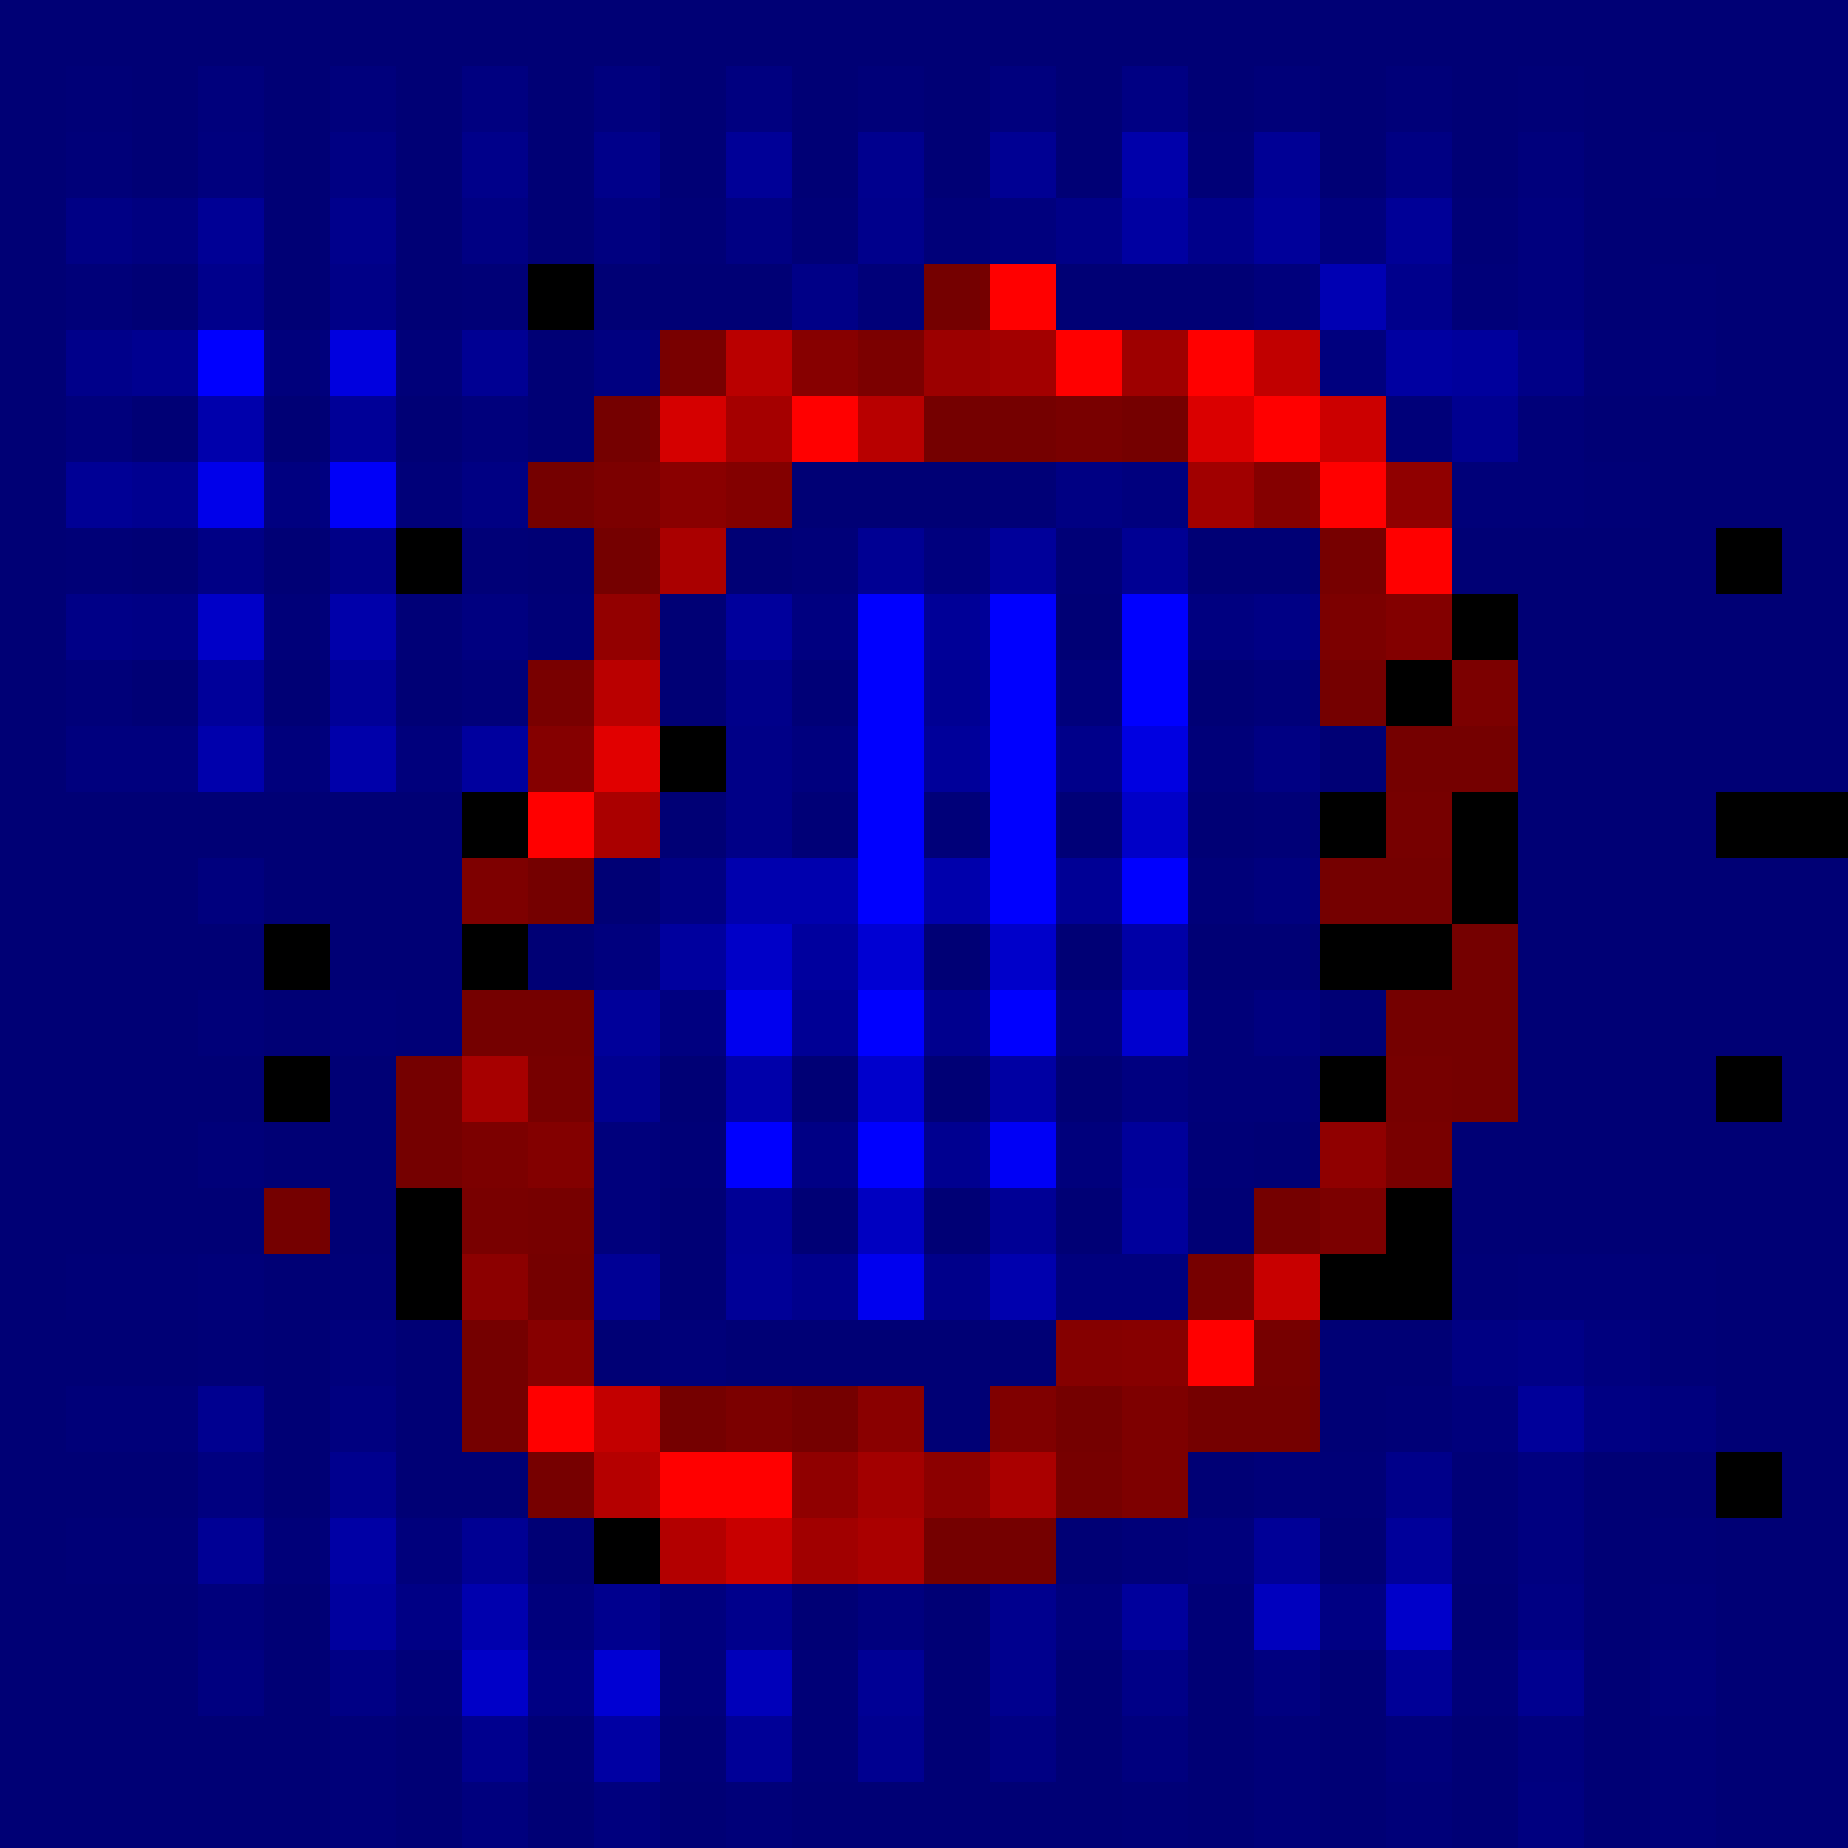
\includegraphics[width=\linewidth]{saliency/mnist_ic_saliency/saliency_threshold_wrt_0_bright.png}
        \scriptsize Gradient 0
    \end{minipage}%
    \begin{minipage}[b]{0.09\linewidth}\centering
        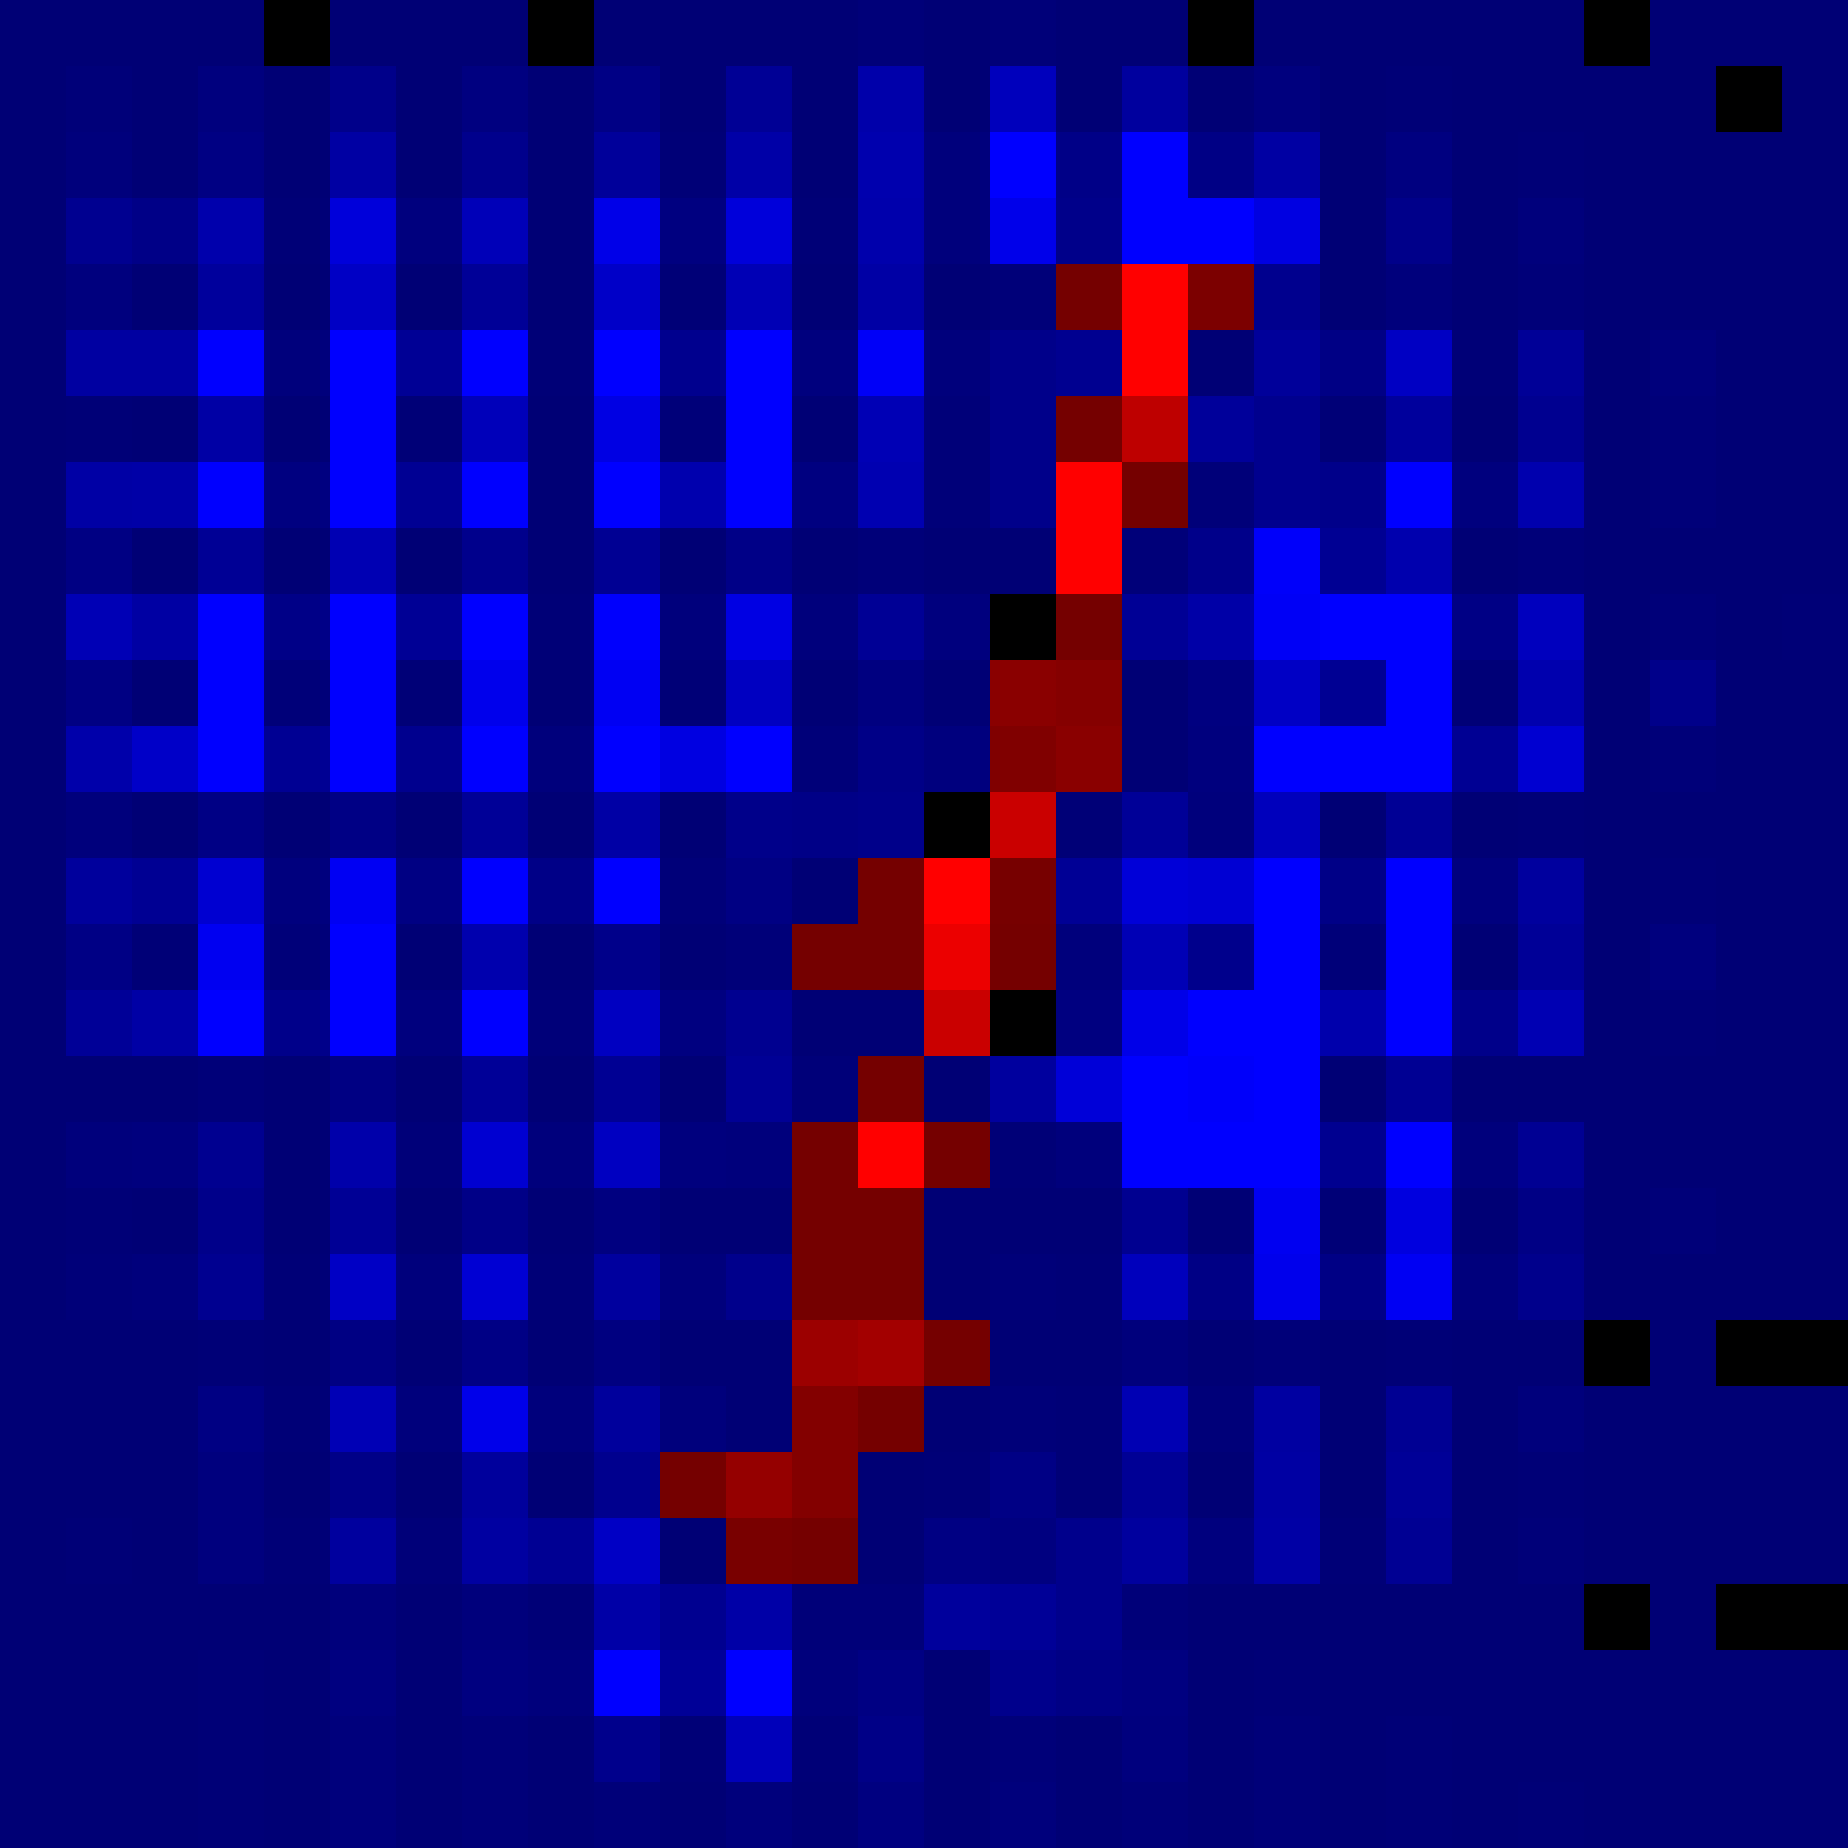
\includegraphics[width=\linewidth]{saliency/mnist_ic_saliency/saliency_threshold_wrt_1_bright.png}
        \scriptsize Gradient 1
    \end{minipage}%
    \begin{minipage}[b]{0.09\linewidth}\centering
        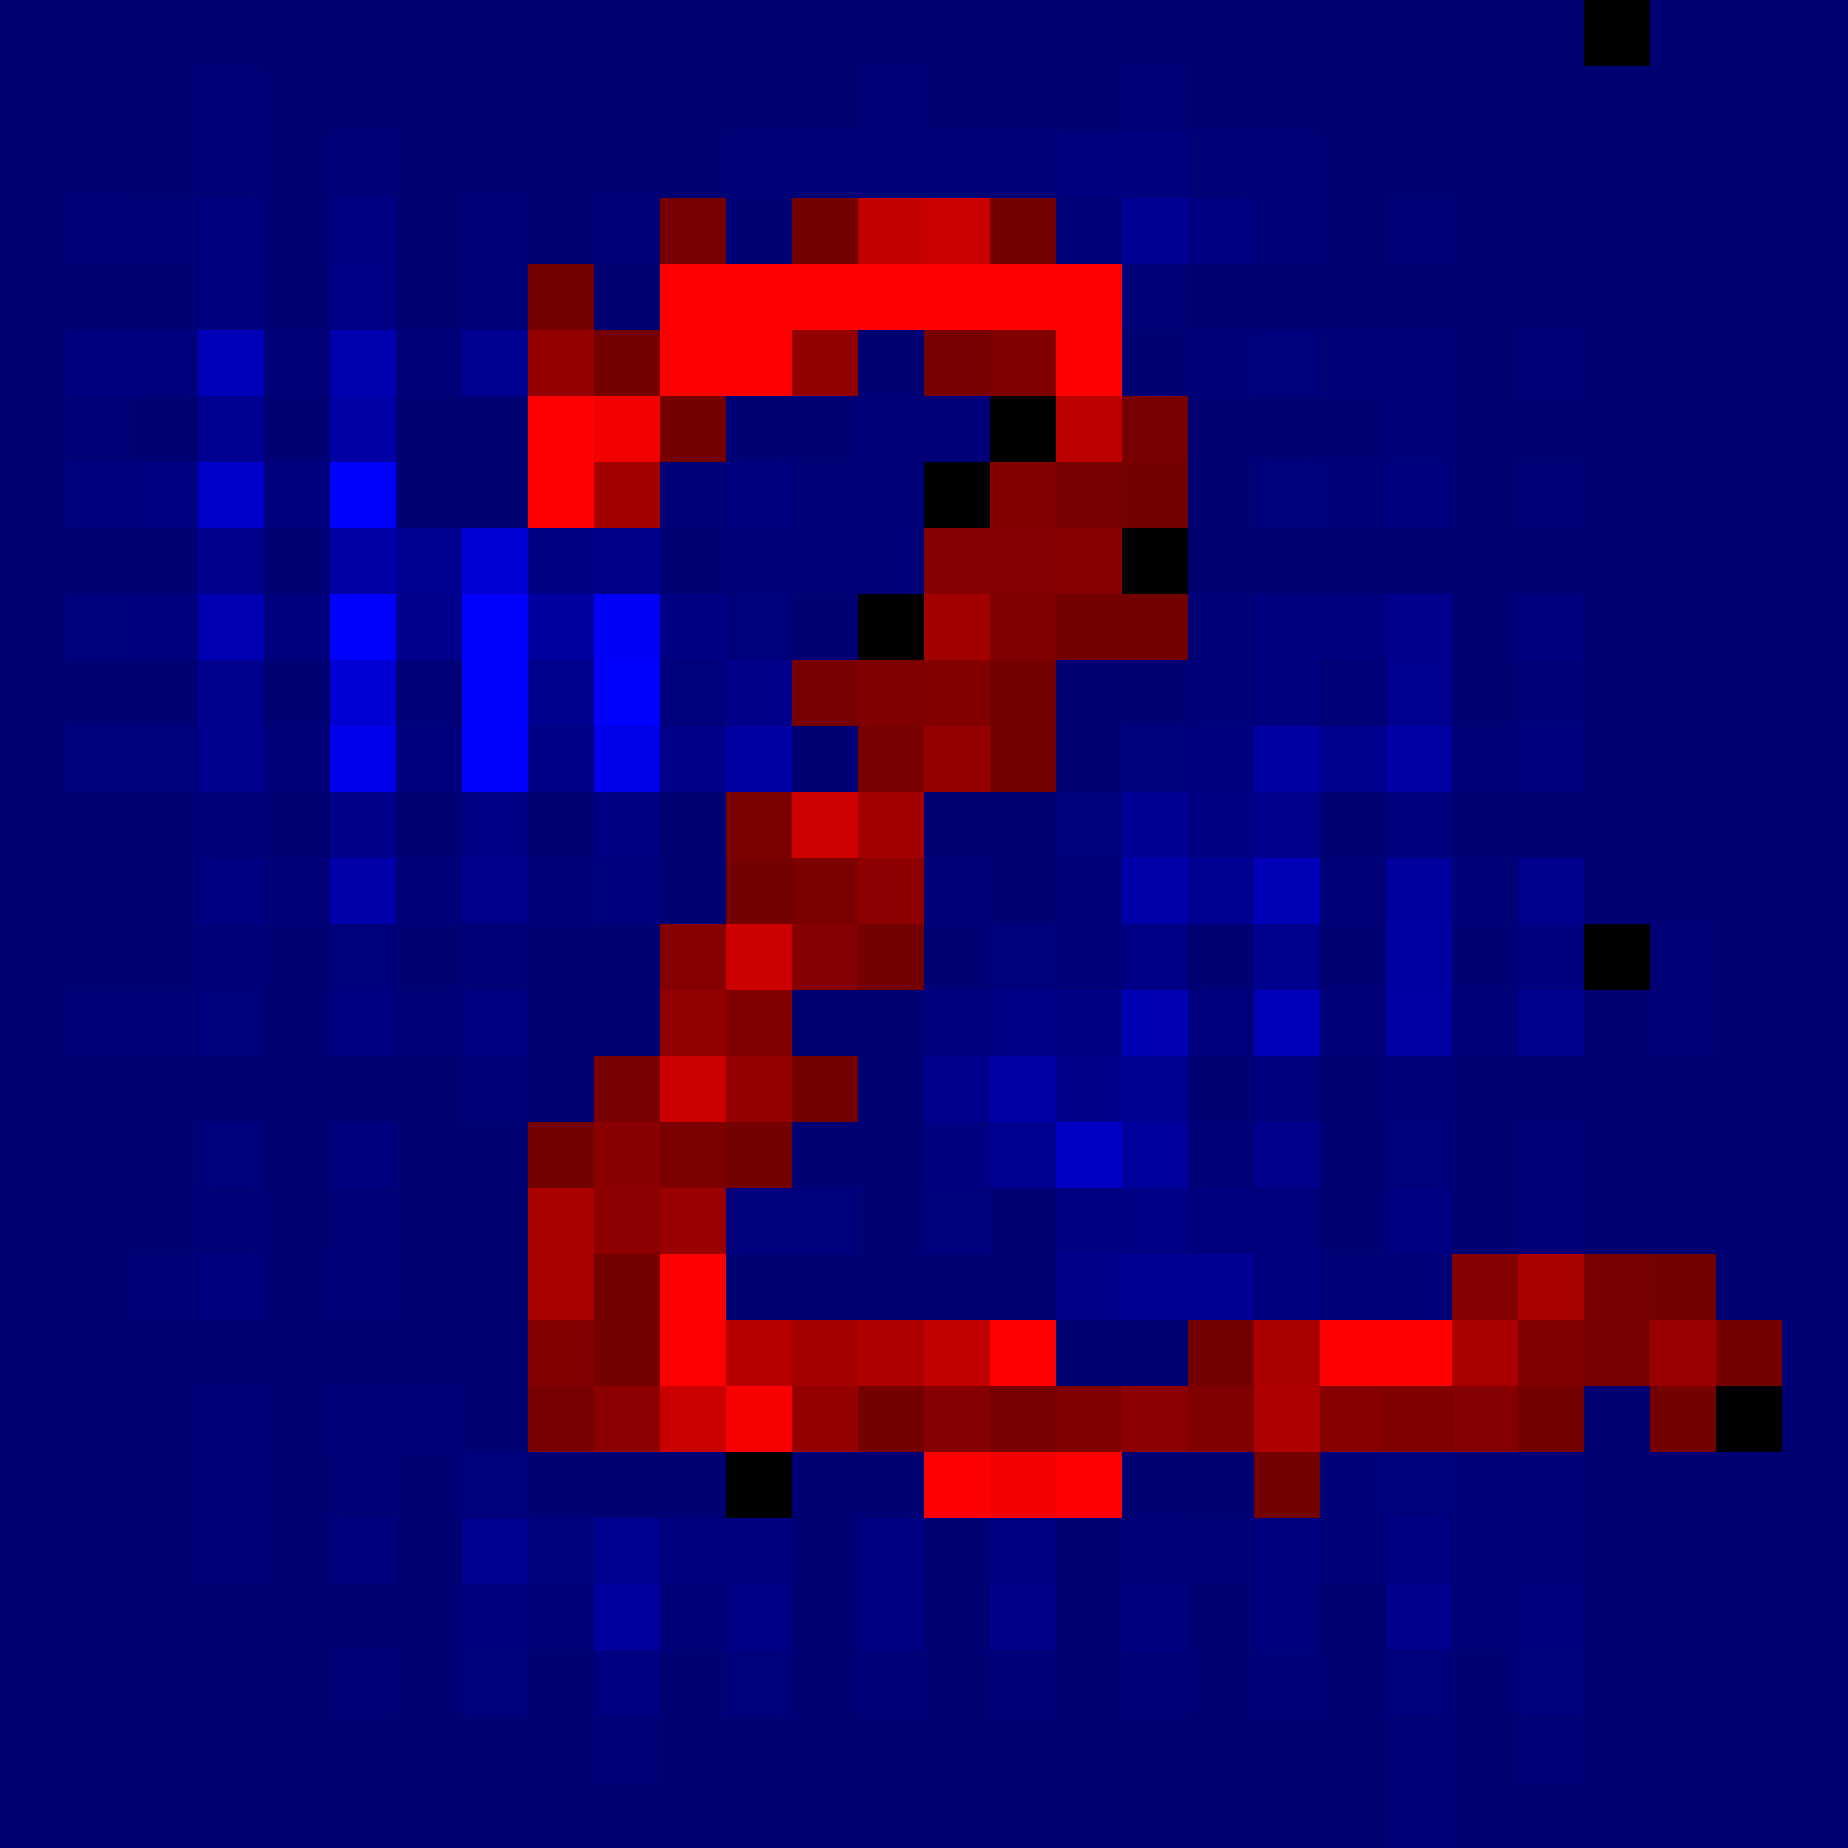
\includegraphics[width=\linewidth]{saliency/mnist_ic_saliency/saliency_threshold_wrt_2_bright.png}
        \scriptsize Gradient 2
    \end{minipage}%
    \begin{minipage}[b]{0.09\linewidth}\centering
        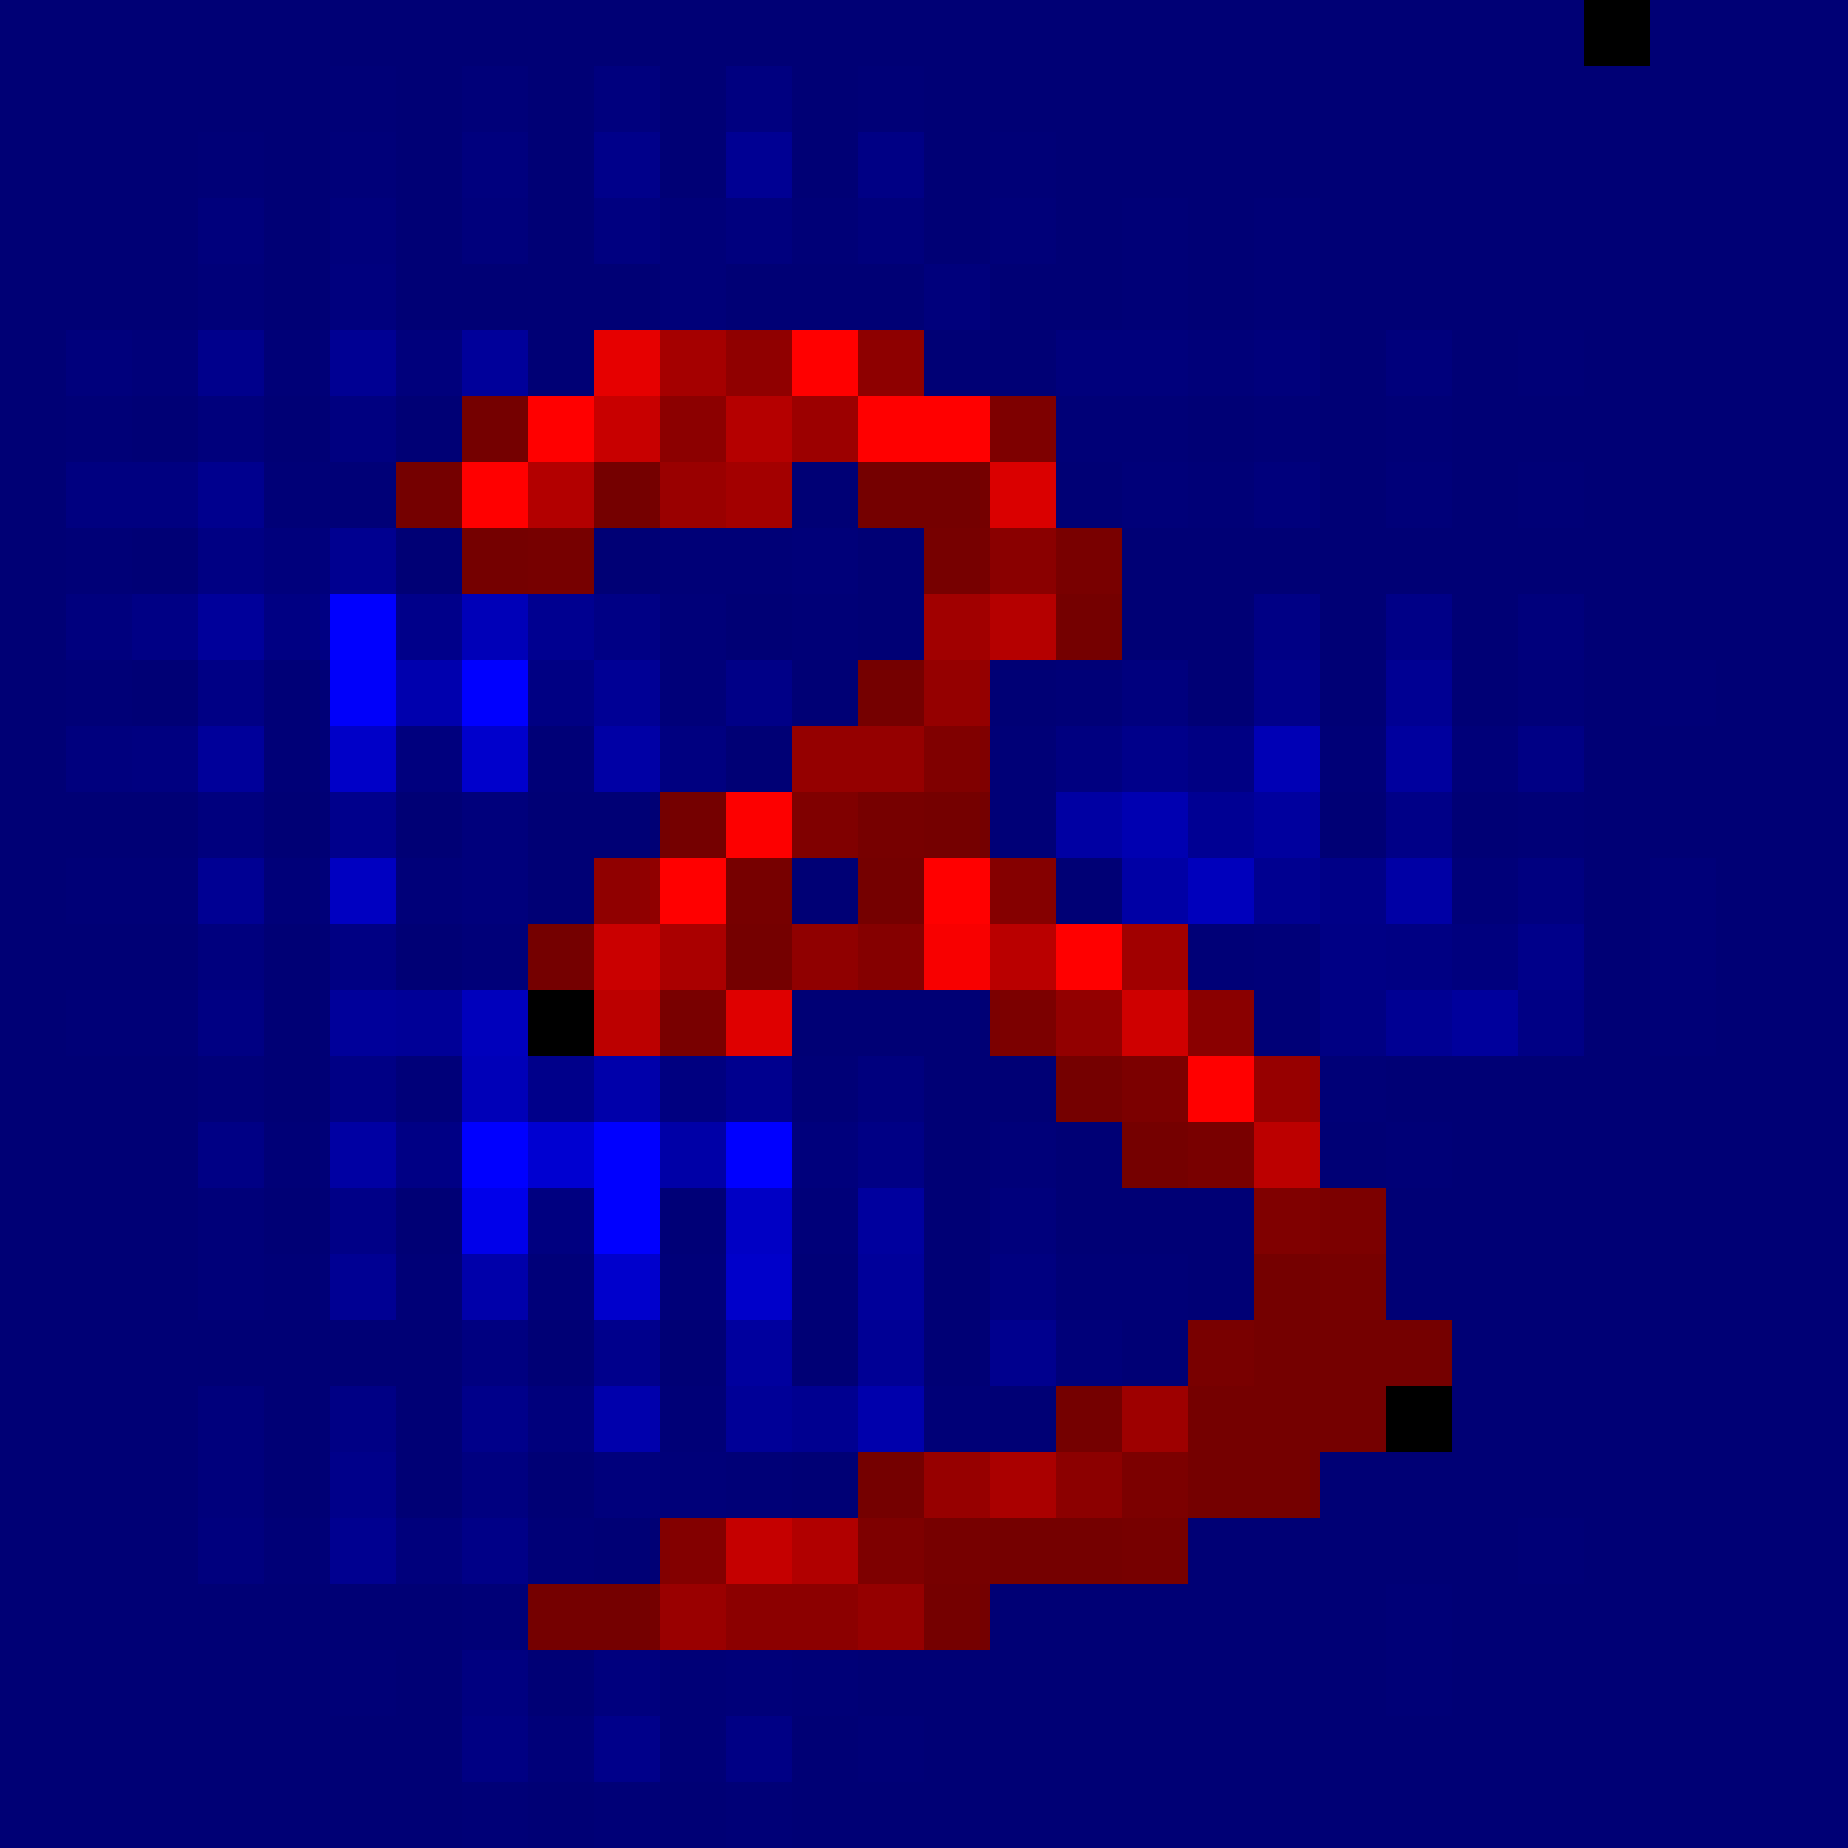
\includegraphics[width=\linewidth]{saliency/mnist_ic_saliency/saliency_threshold_wrt_3_bright.png}
        \scriptsize Gradient 3
    \end{minipage}%
    \begin{minipage}[b]{0.09\linewidth}\centering
        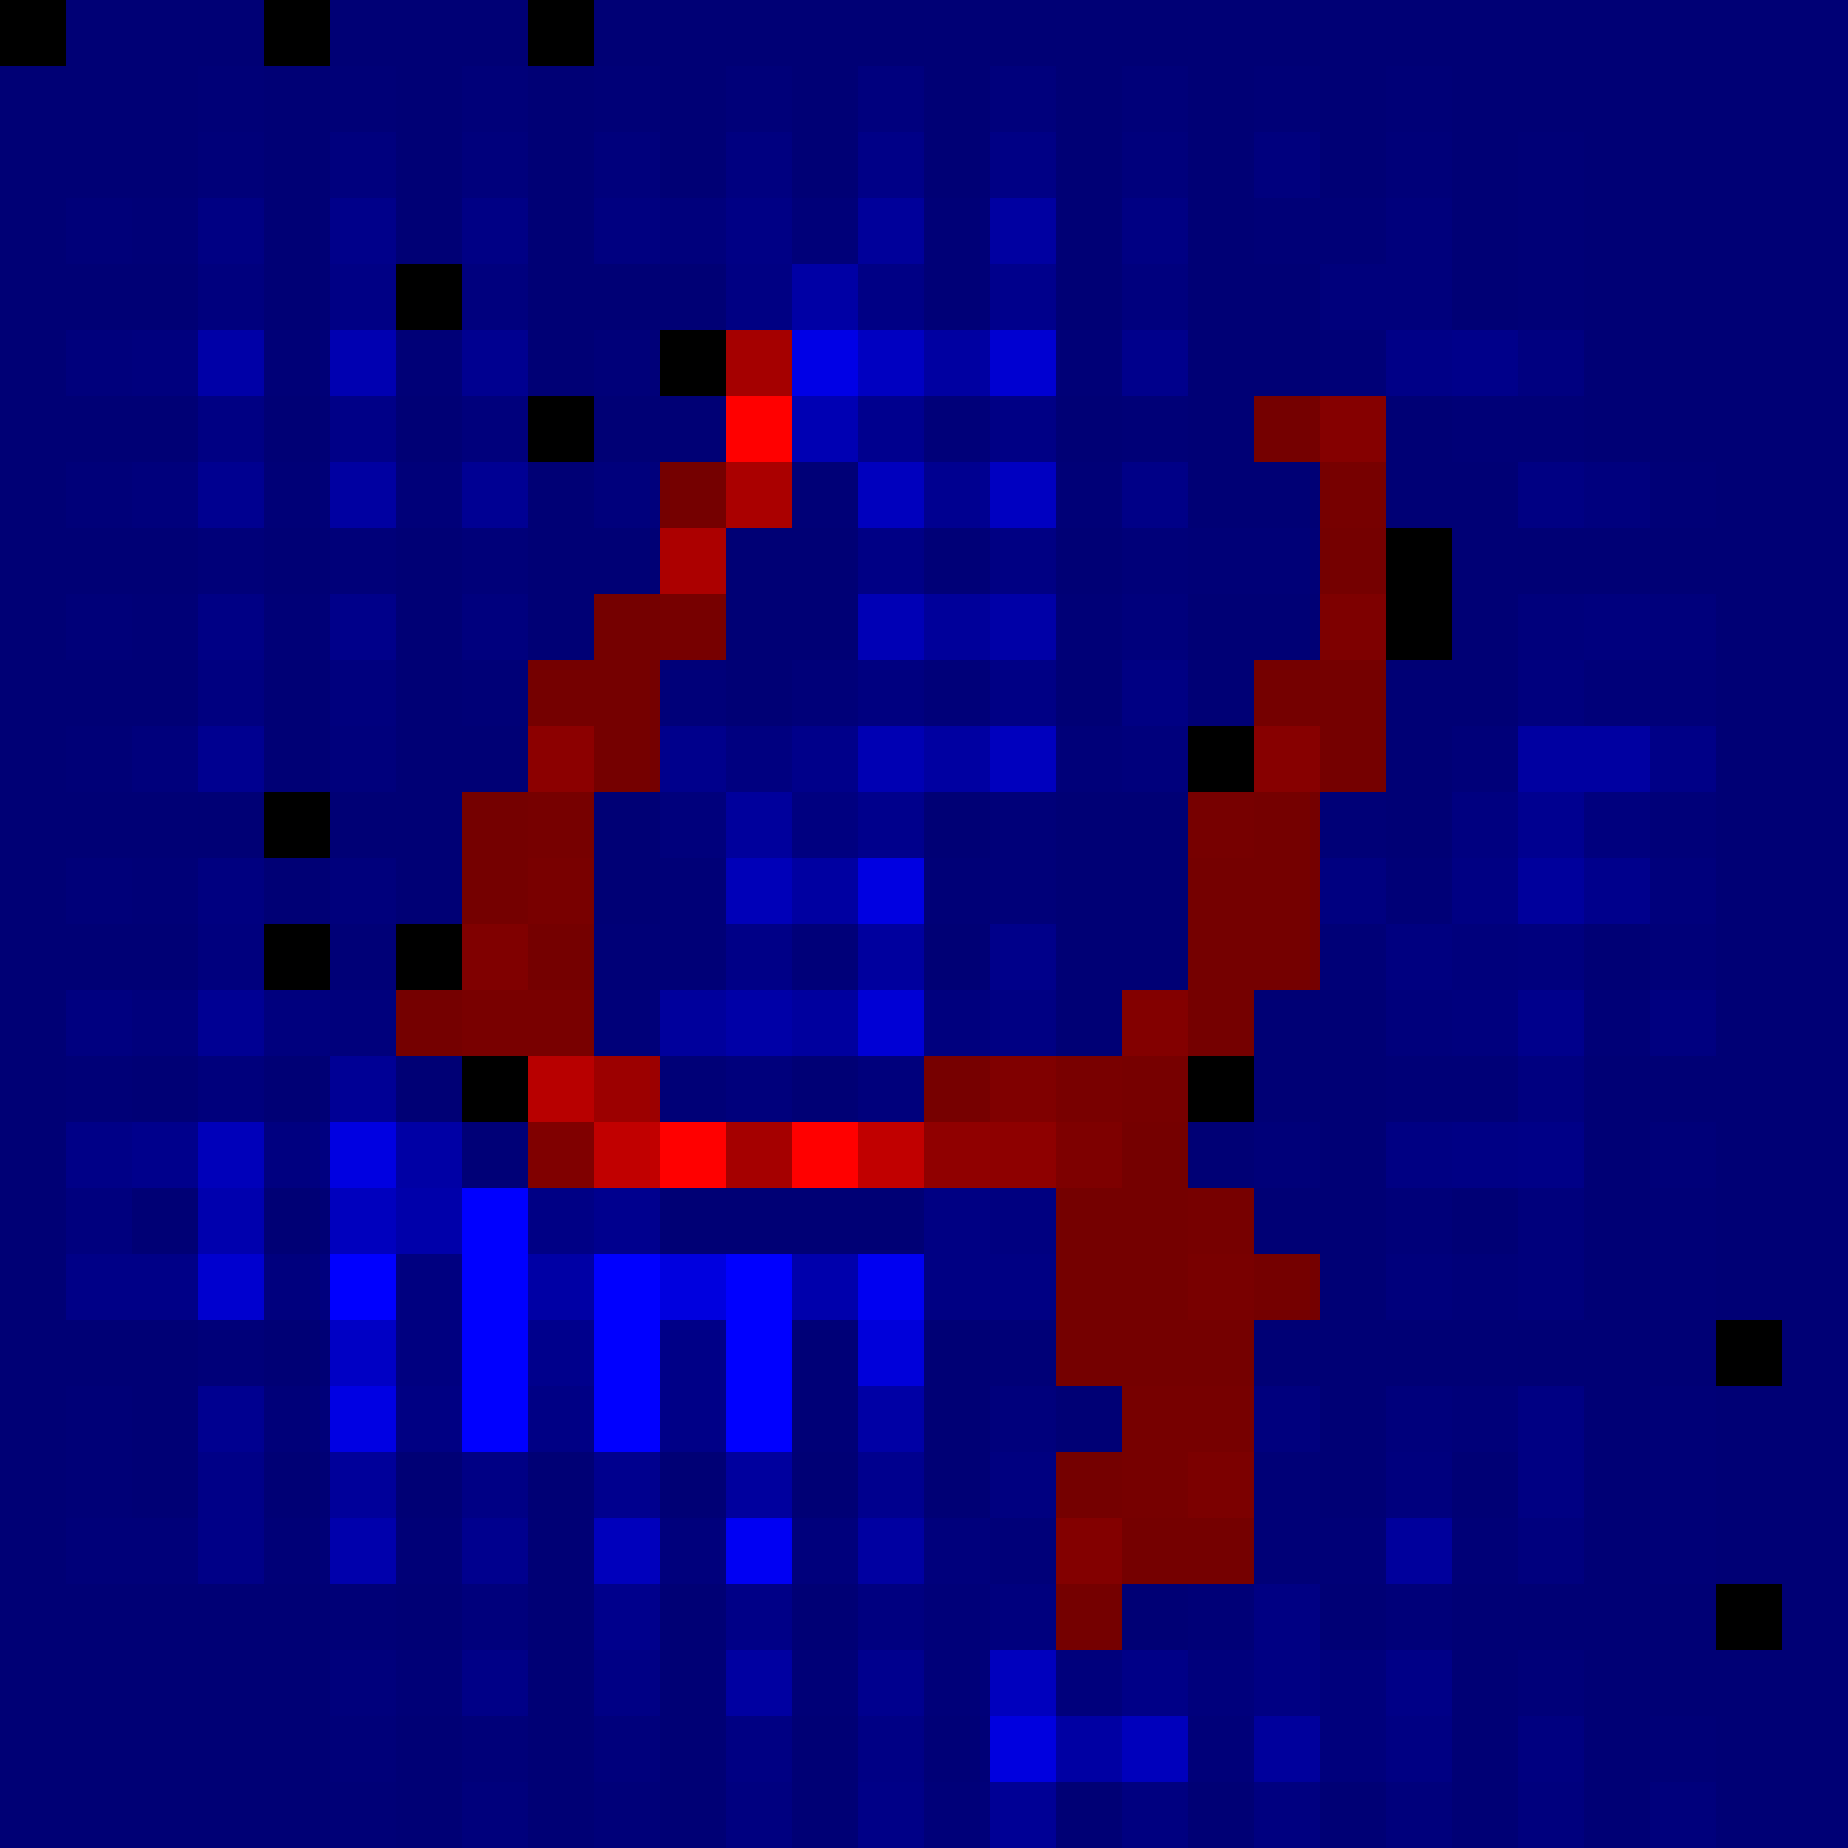
\includegraphics[width=\linewidth]{saliency/mnist_ic_saliency/saliency_threshold_wrt_4_bright.png}
        \scriptsize Gradient 4
    \end{minipage}%
    \begin{minipage}[b]{0.09\linewidth}\centering
        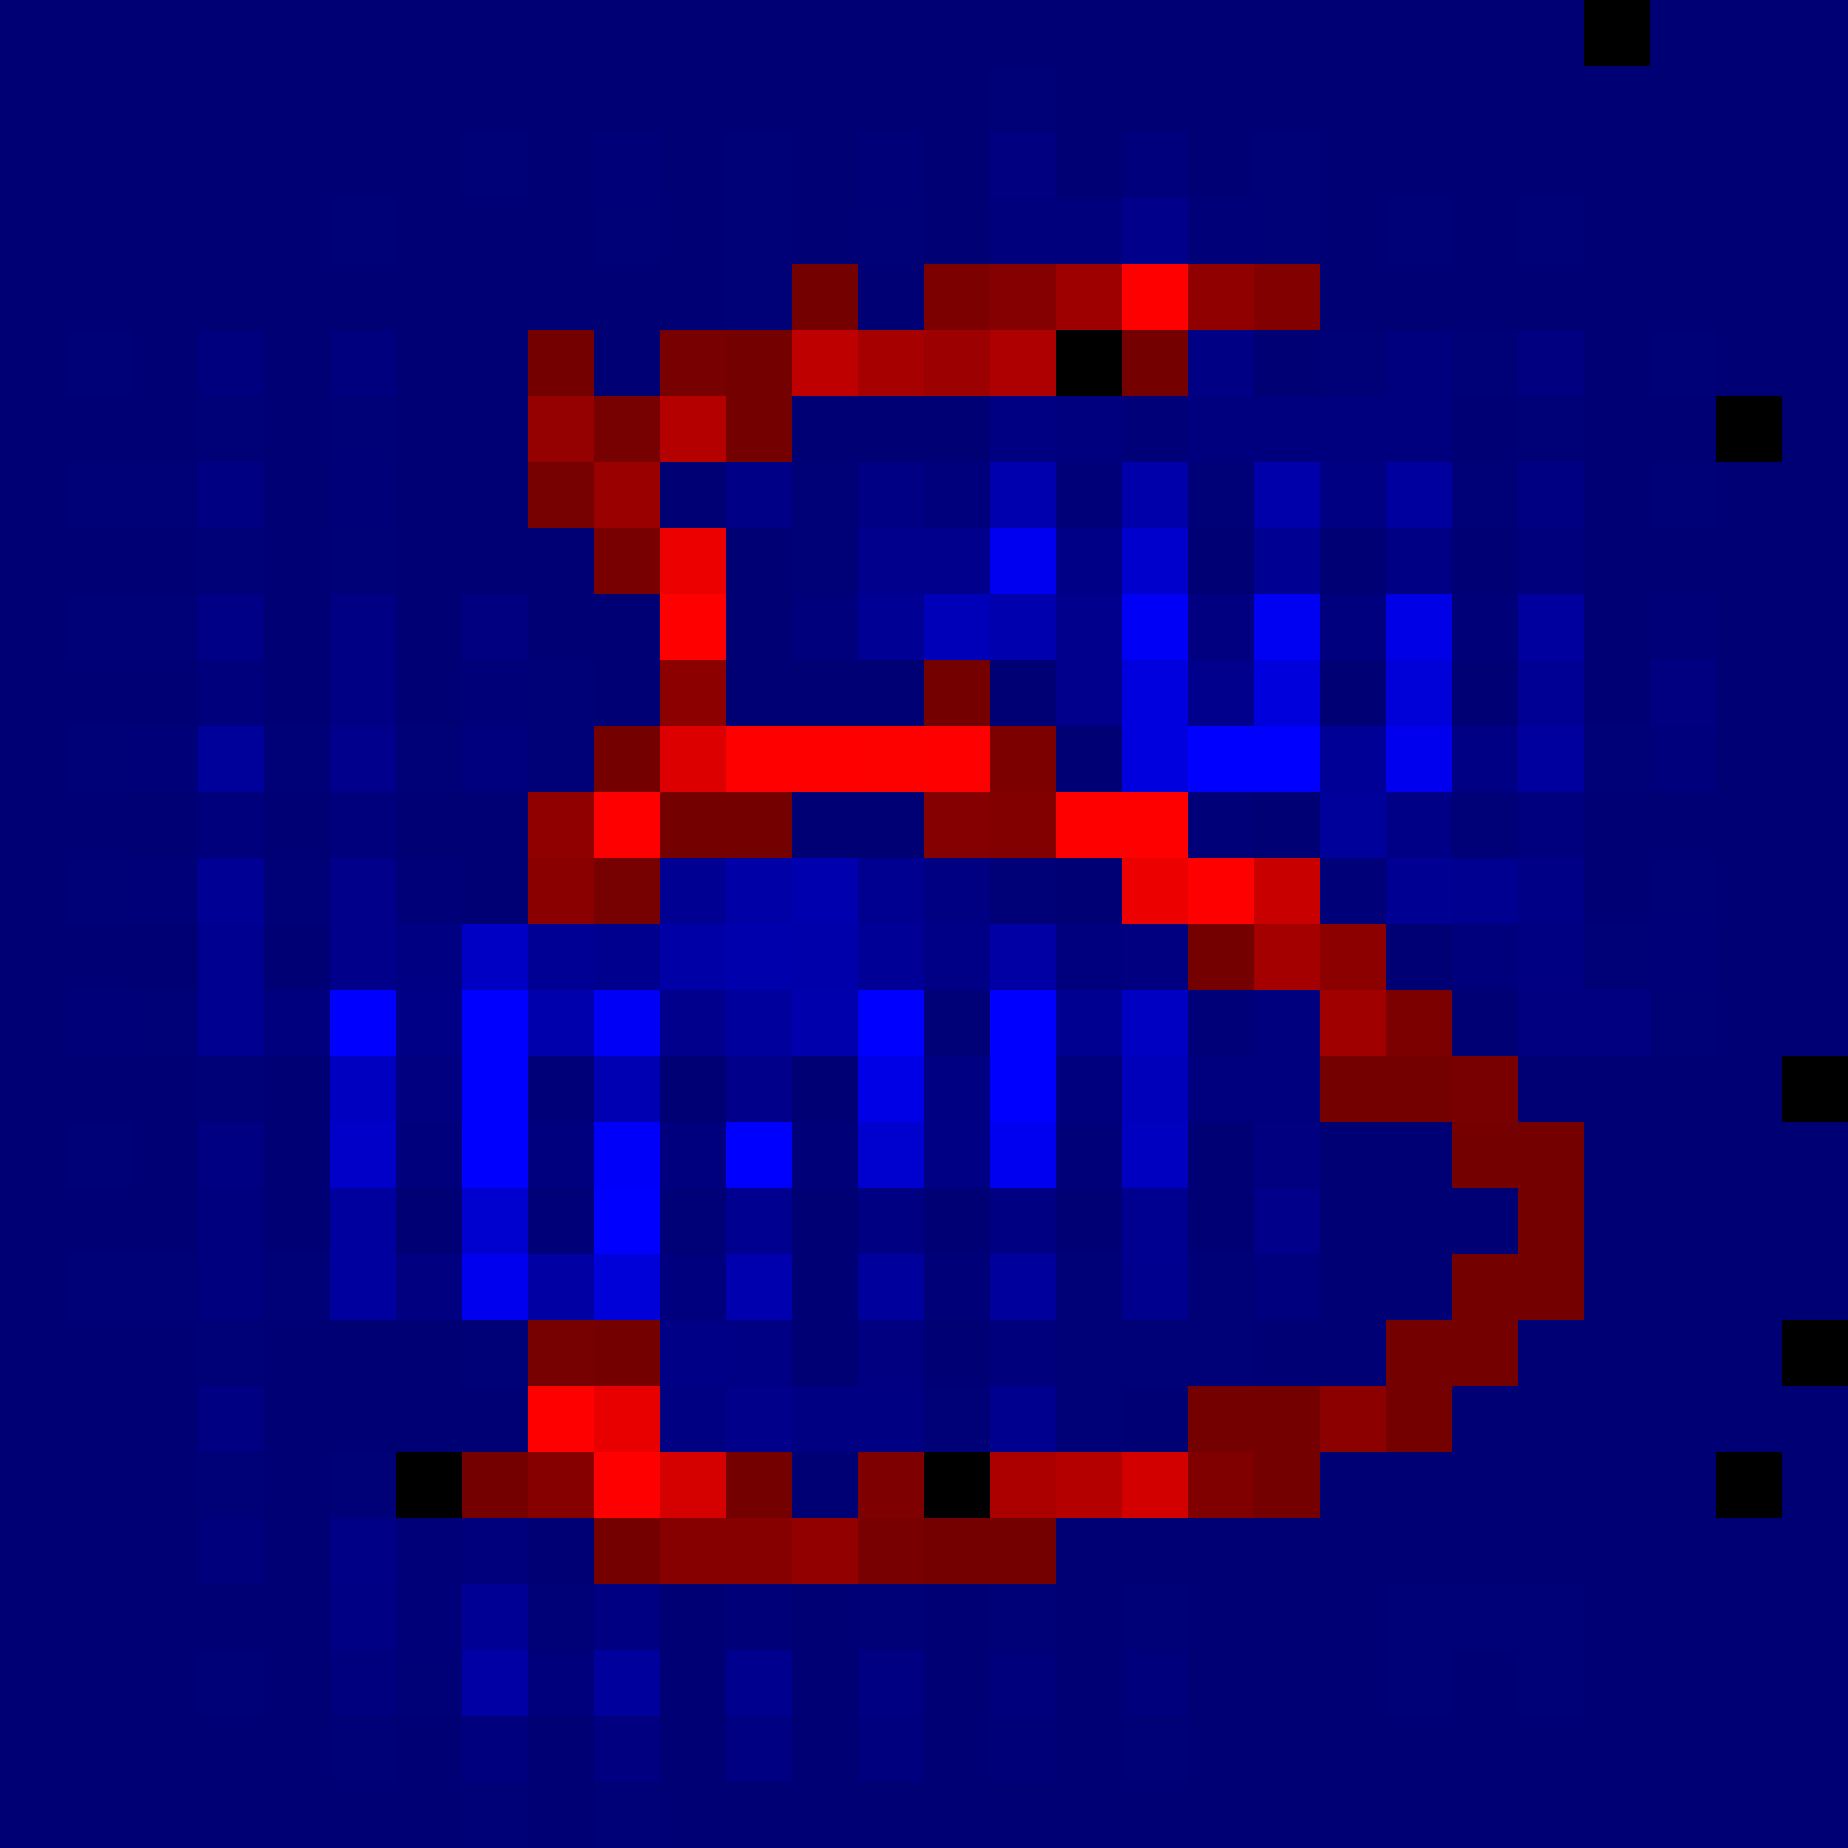
\includegraphics[width=\linewidth]{saliency/mnist_ic_saliency/saliency_threshold_wrt_5_bright.png}
        \scriptsize Gradient 5
    \end{minipage}%
    \begin{minipage}[b]{0.09\linewidth}\centering
        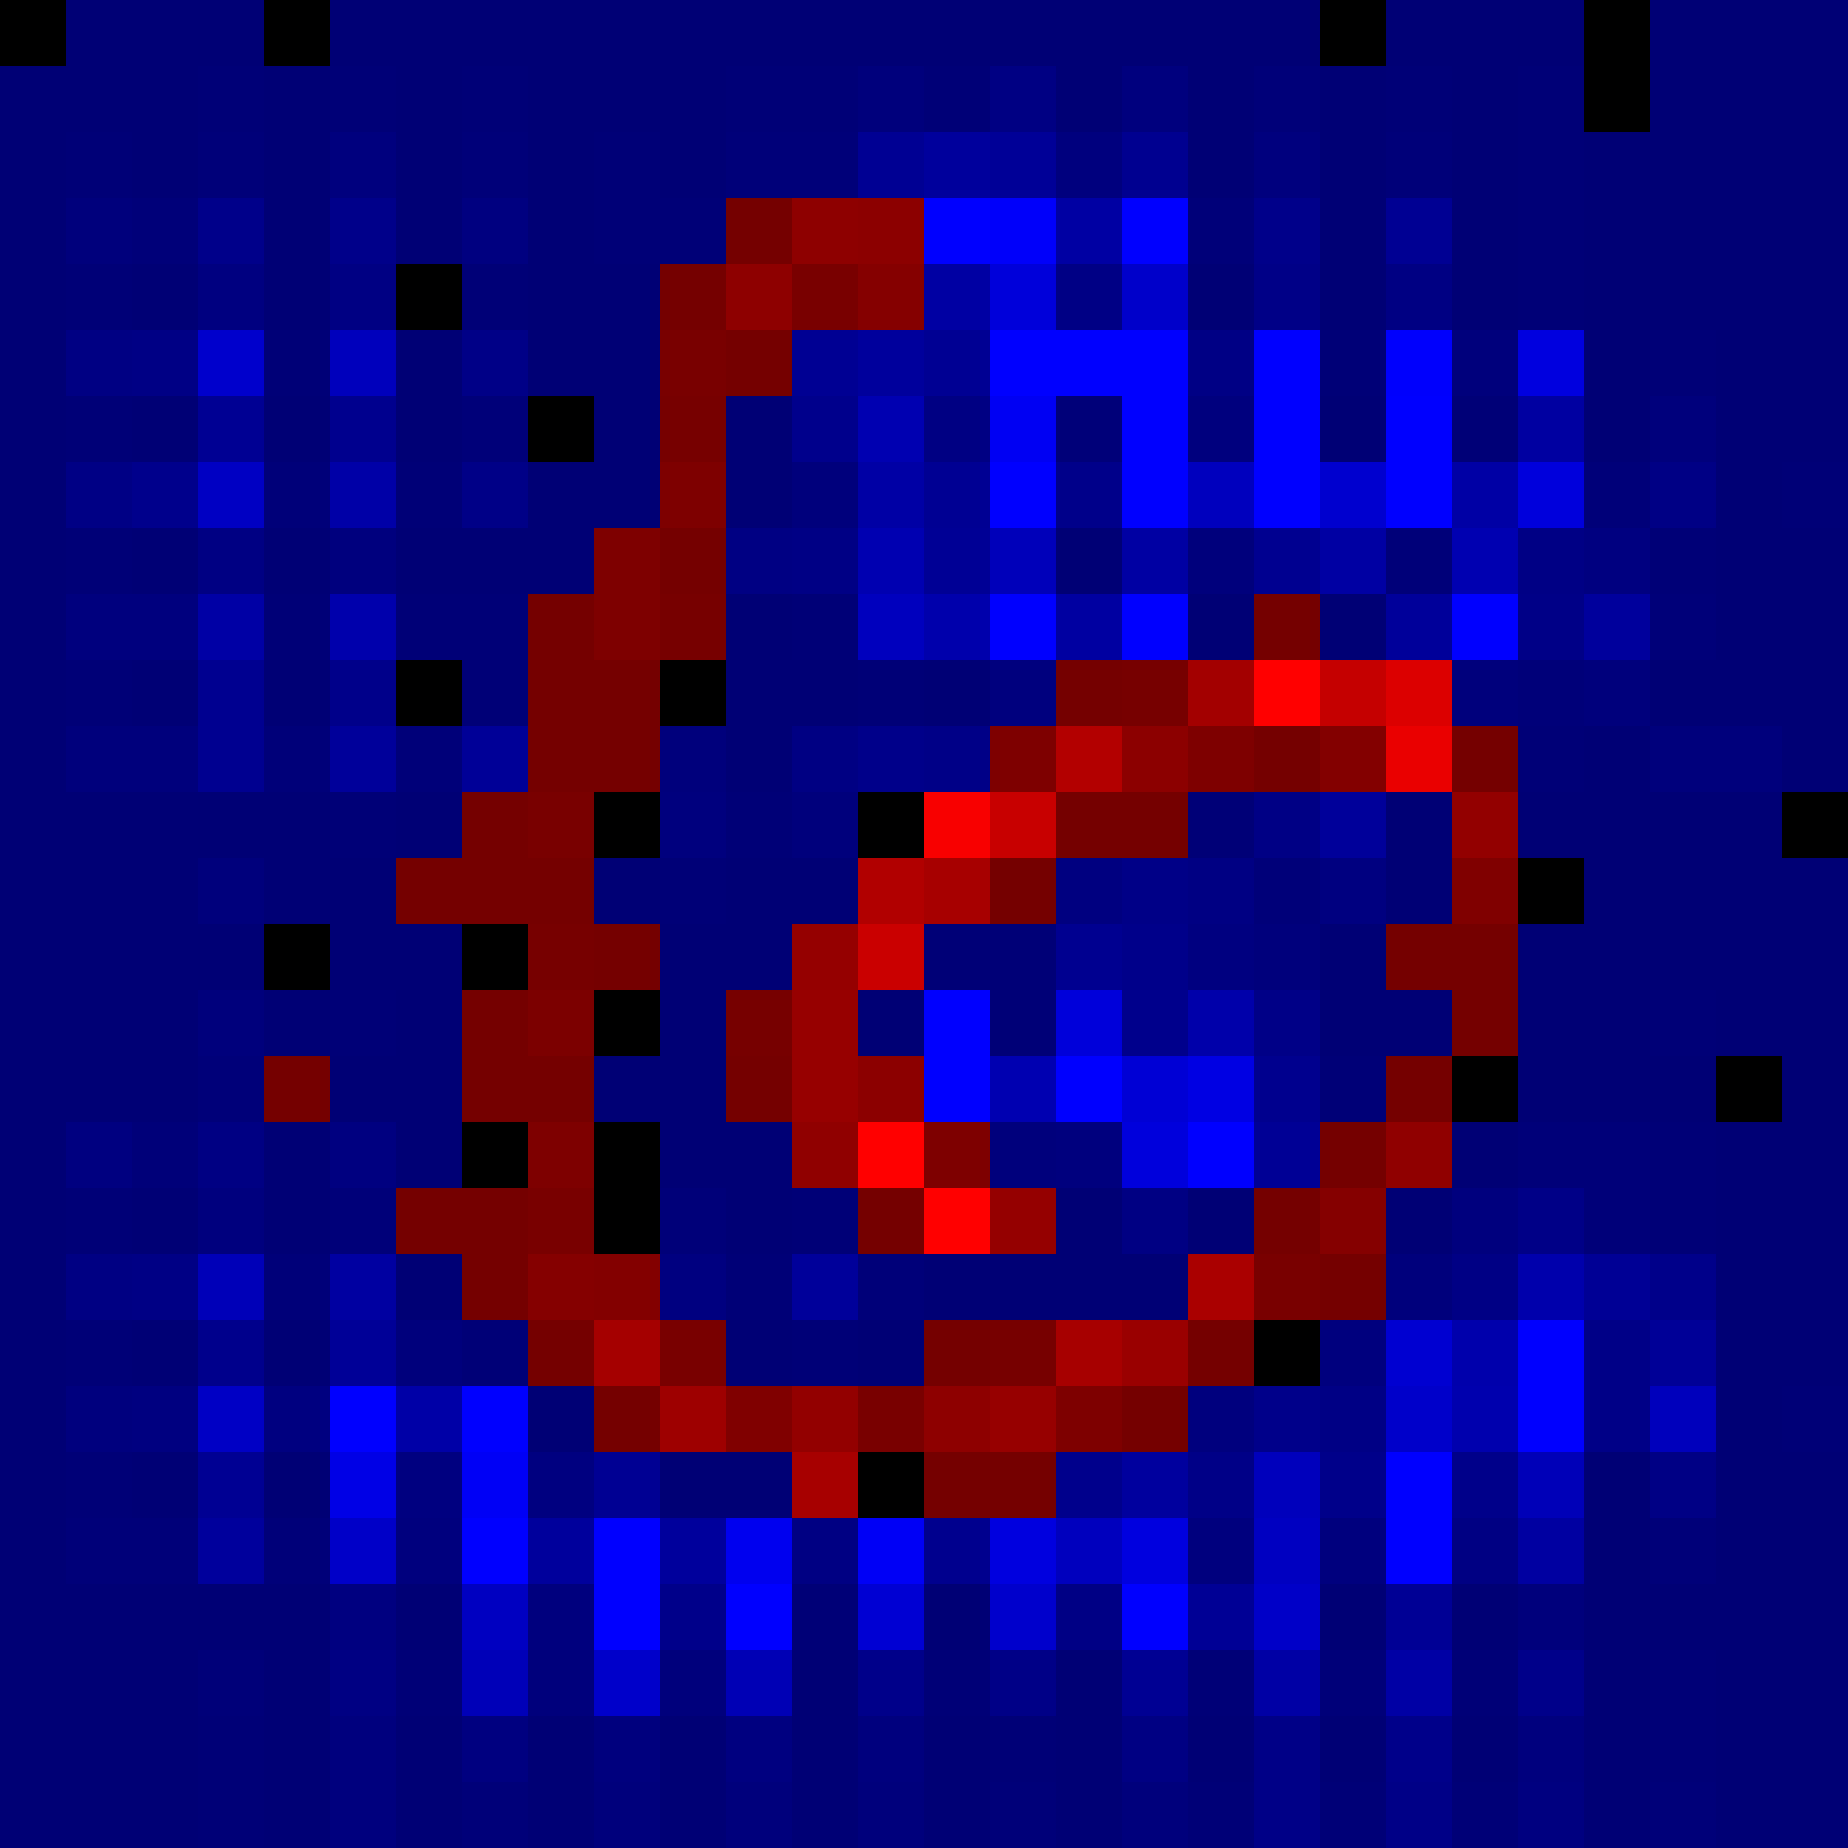
\includegraphics[width=\linewidth]{saliency/mnist_ic_saliency/saliency_threshold_wrt_6_bright.png}
        \scriptsize Gradient 6
    \end{minipage}%
    \begin{minipage}[b]{0.09\linewidth}\centering
        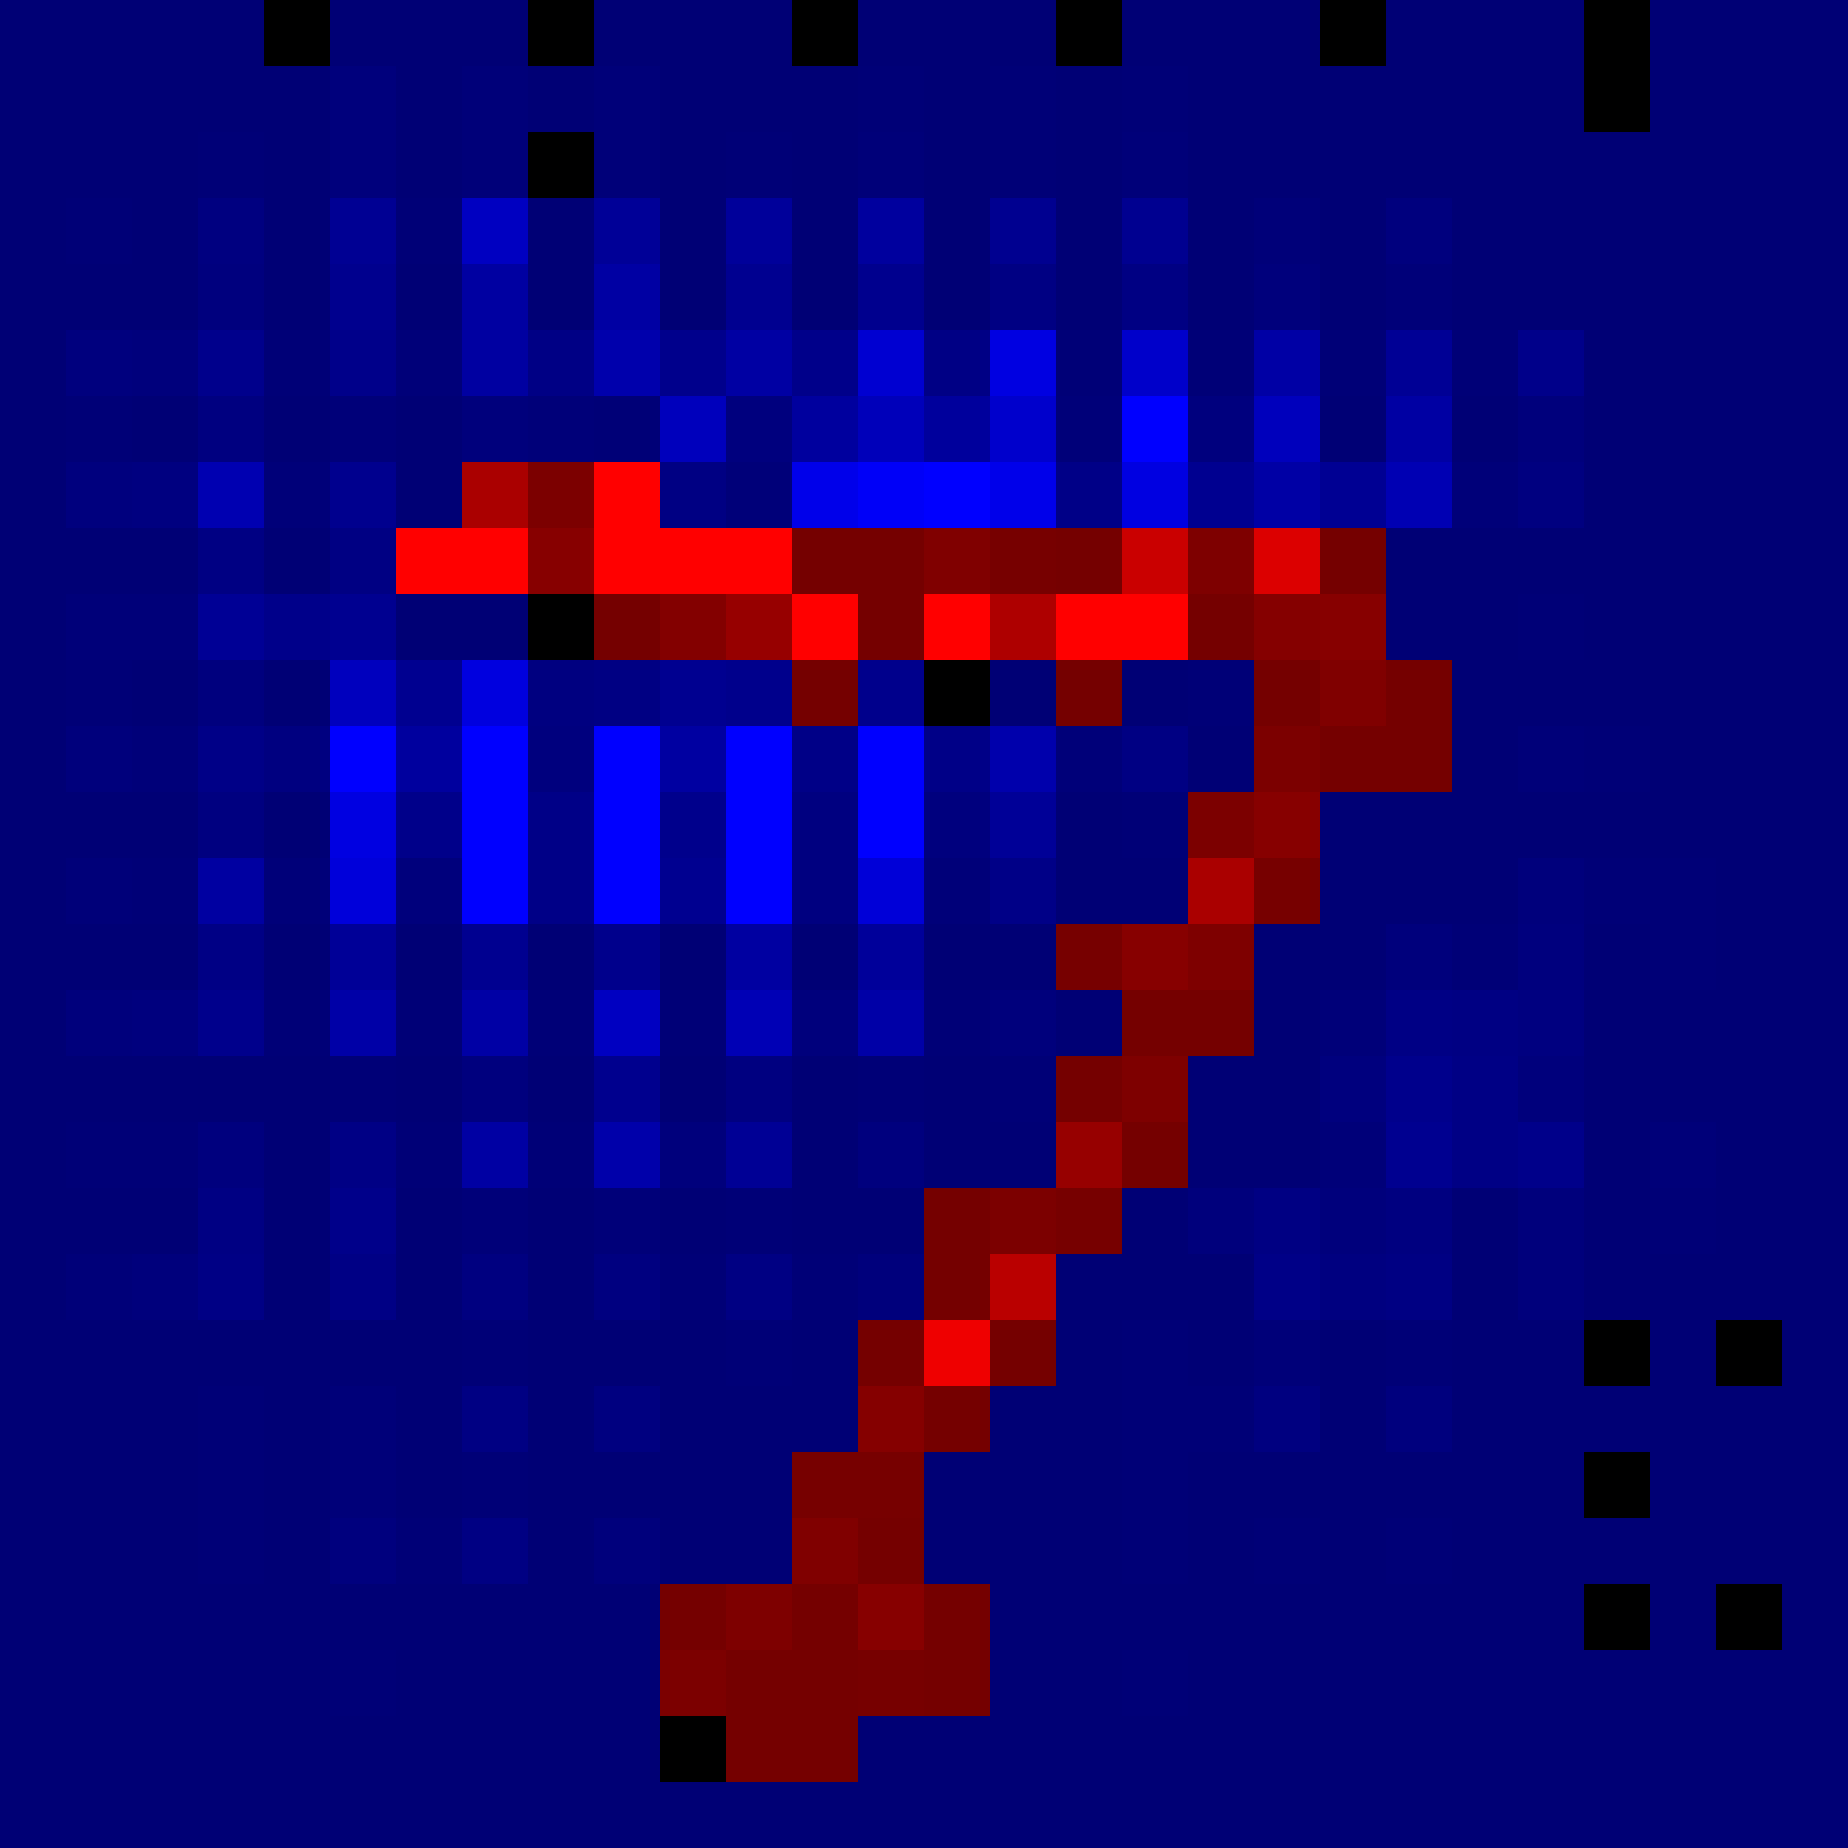
\includegraphics[width=\linewidth]{saliency/mnist_ic_saliency/saliency_threshold_wrt_7_bright.png}
        \scriptsize Gradient 7
    \end{minipage}%
    \begin{minipage}[b]{0.09\linewidth}\centering
        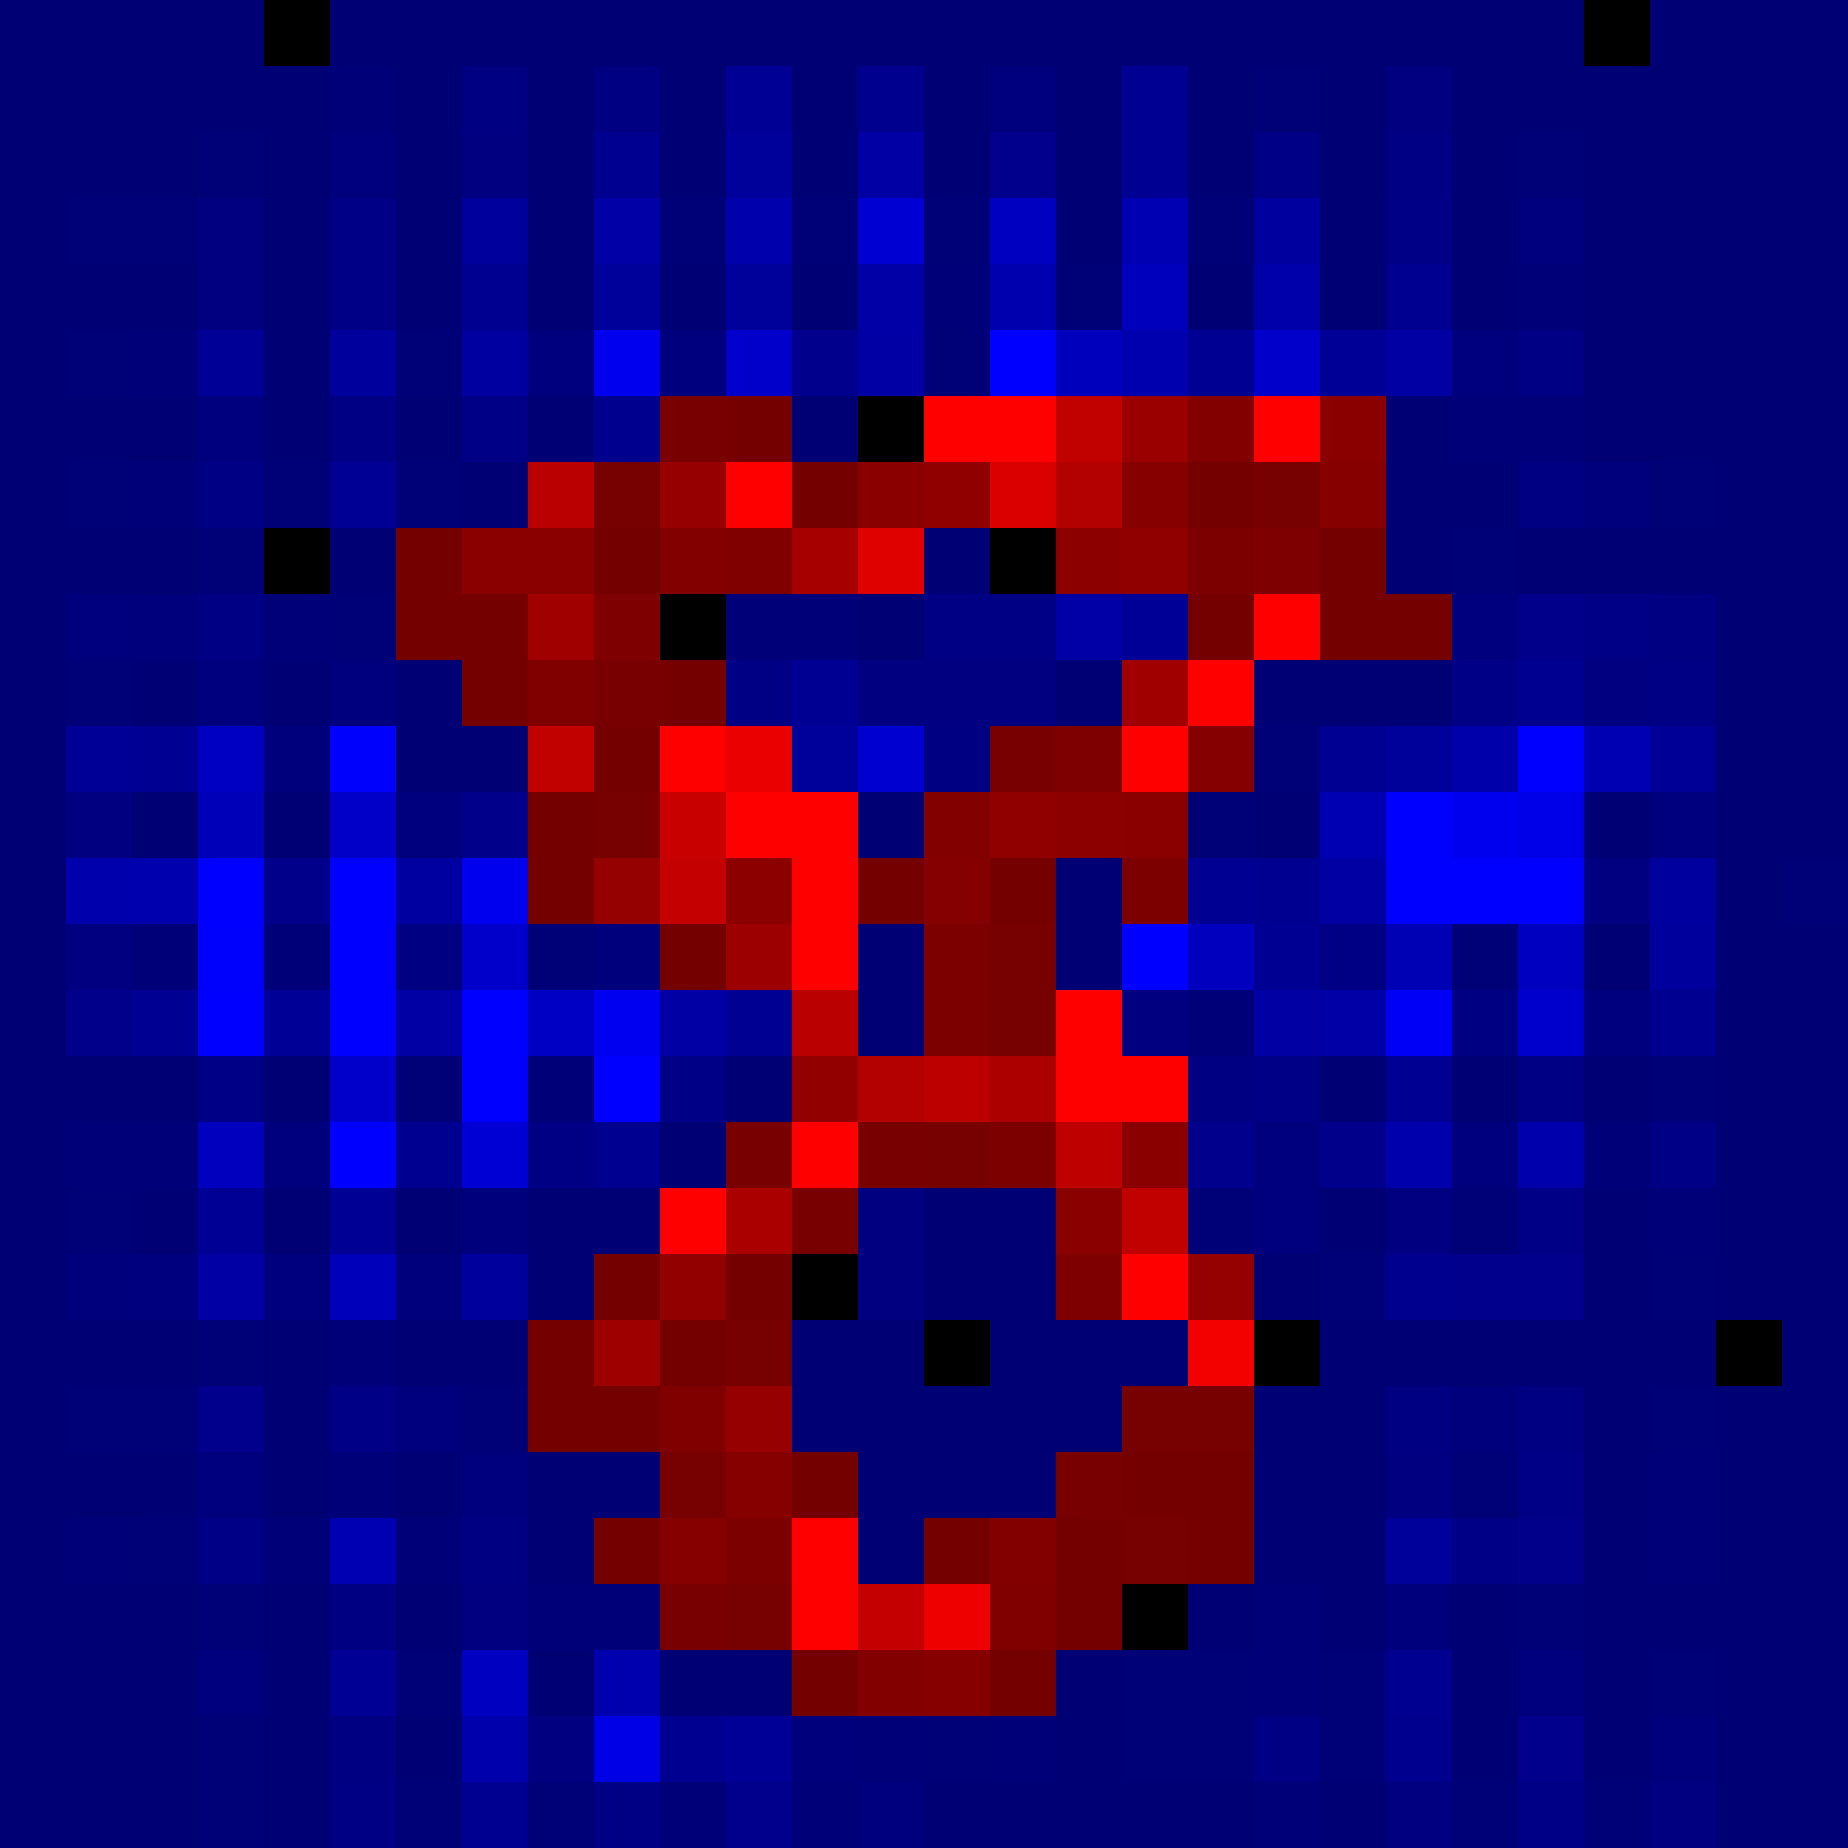
\includegraphics[width=\linewidth]{saliency/mnist_ic_saliency/saliency_threshold_wrt_8_bright.png}
        \scriptsize Gradient 8
    \end{minipage}%
    \begin{minipage}[b]{0.09\linewidth}\centering
        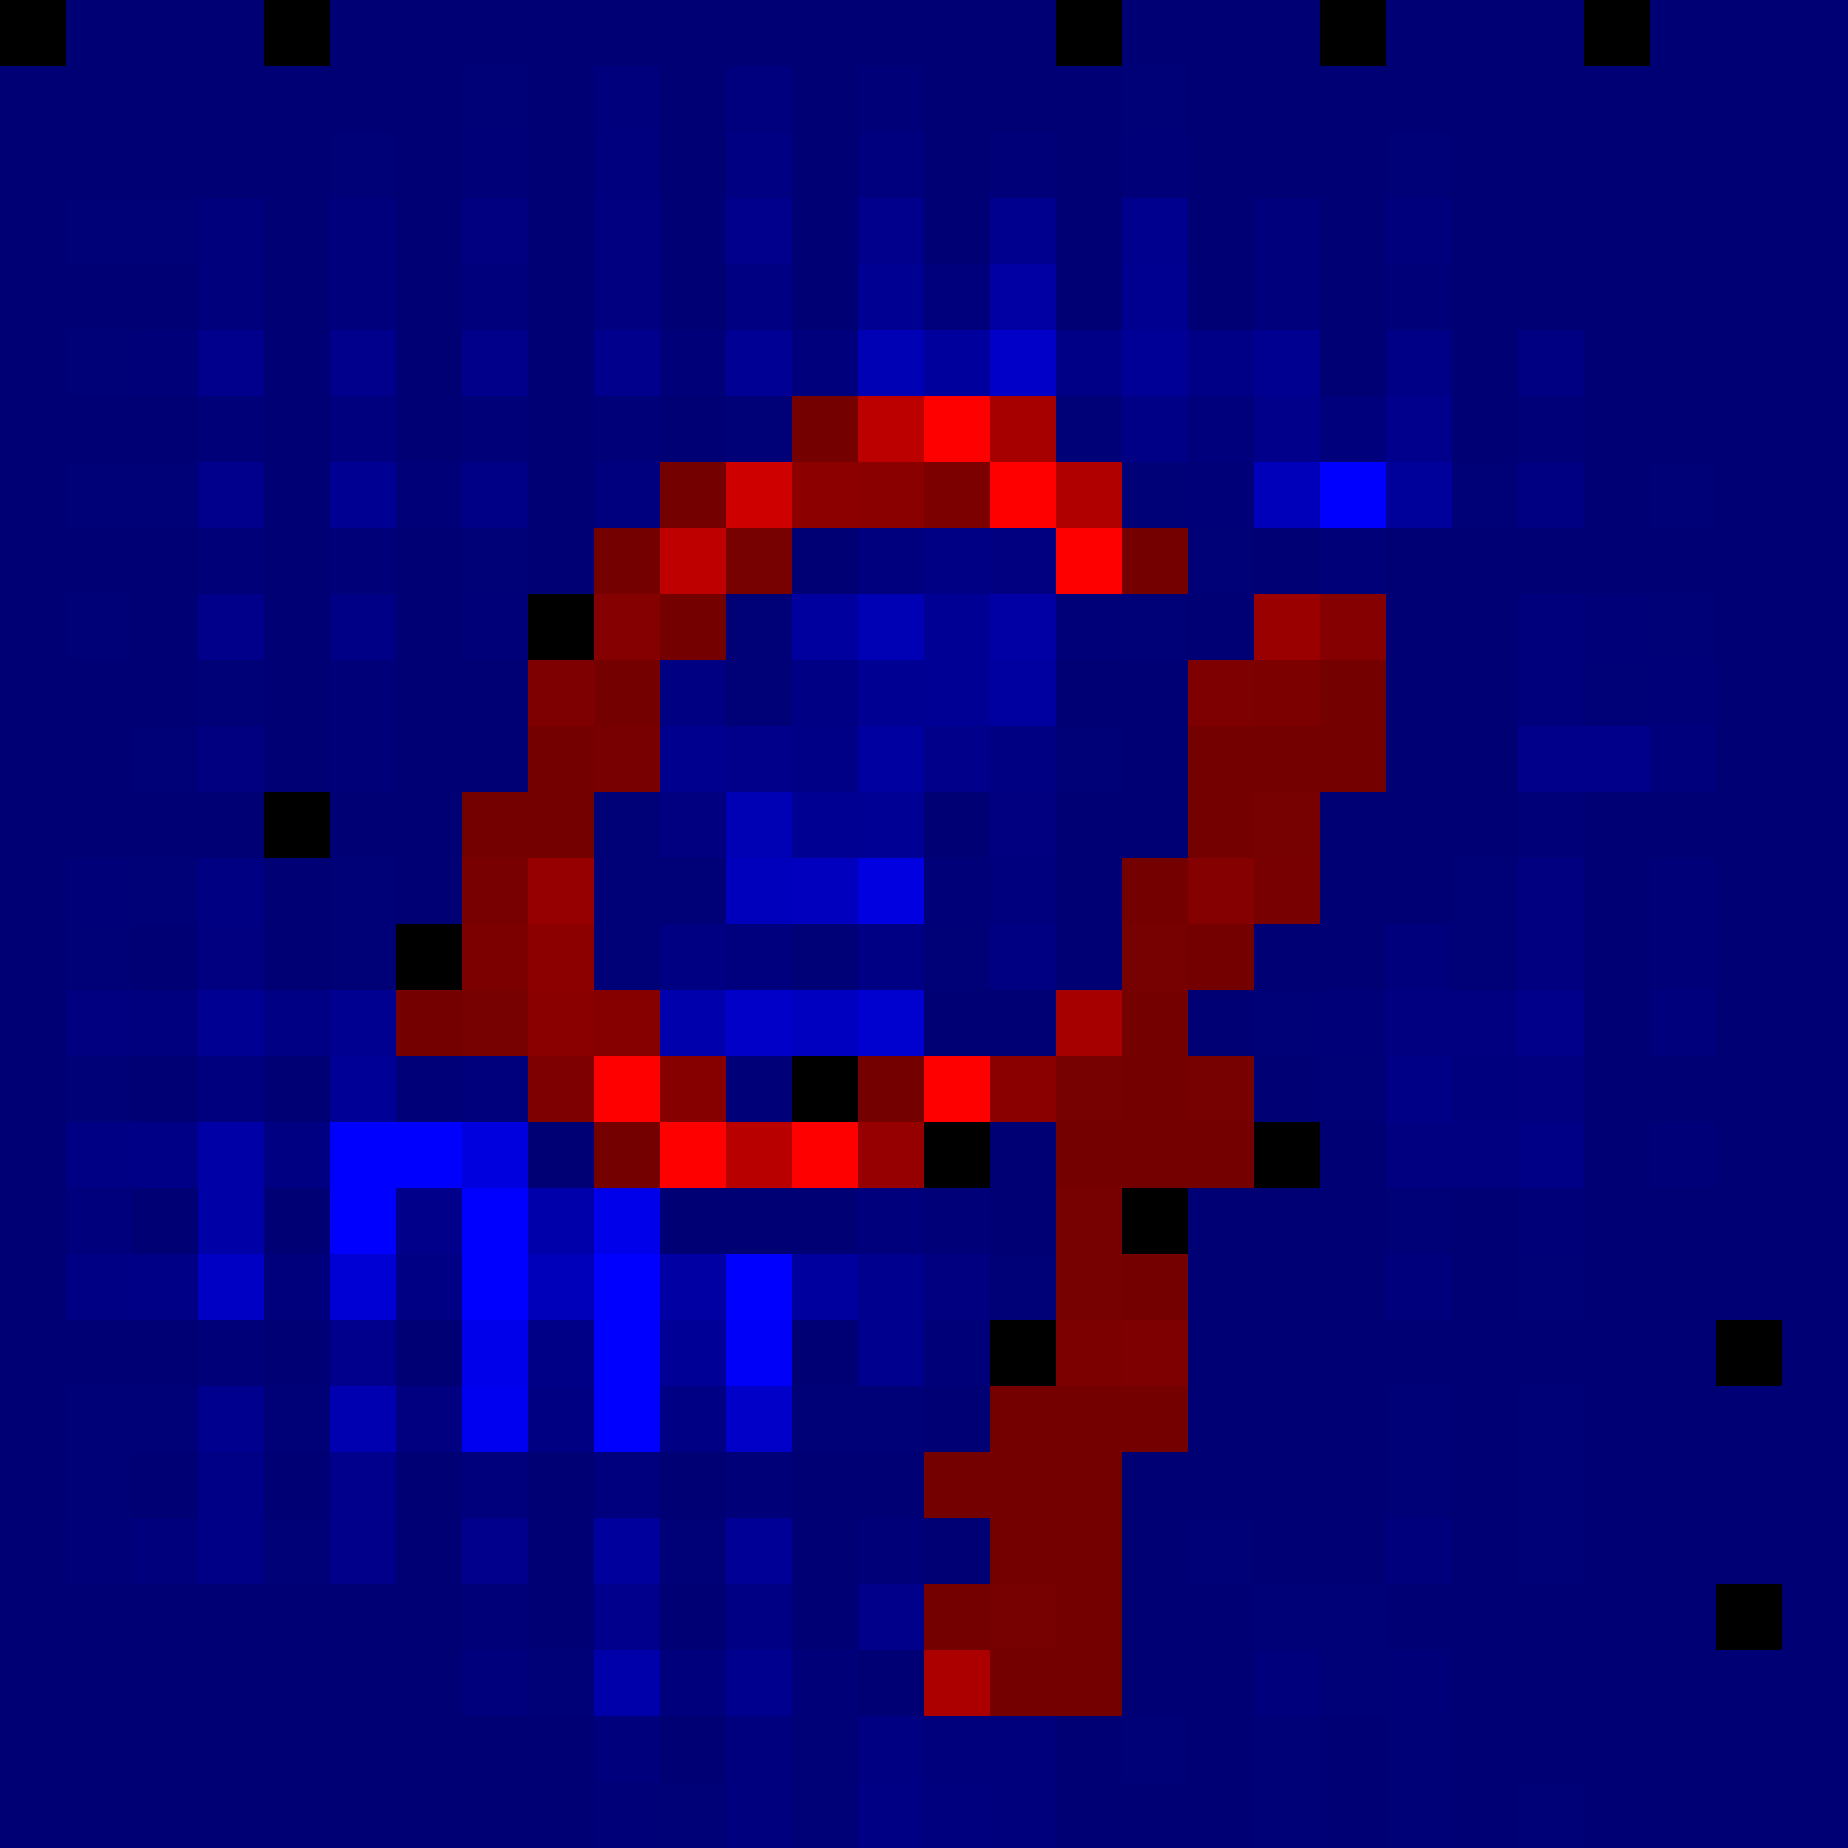
\includegraphics[width=\linewidth]{saliency/mnist_ic_saliency/saliency_threshold_wrt_9_bright.png}
        \scriptsize Gradient 9
    \end{minipage}%

    \par\vspace{0.25cm}
    \begin{minipage}[b]{0.09\linewidth}\centering
        
\includegraphics[width=\linewidth]{saliency/mnist_ic_saliency/original_0.png}
        \scriptsize Label 0
    \end{minipage}%
    \begin{minipage}[b]{0.09\linewidth}\centering
        
\includegraphics[width=\linewidth]{saliency/mnist_ic_saliency/original_1.png}
        \scriptsize Label 1
    \end{minipage}%
    \begin{minipage}[b]{0.09\linewidth}\centering
        
\includegraphics[width=\linewidth]{saliency/mnist_ic_saliency/original_2.png}
        \scriptsize Label 2
    \end{minipage}%
    \begin{minipage}[b]{0.09\linewidth}\centering
        
\includegraphics[width=\linewidth]{saliency/mnist_ic_saliency/original_3.png}
        \scriptsize Label 3
    \end{minipage}%
    \begin{minipage}[b]{0.09\linewidth}\centering
        
\includegraphics[width=\linewidth]{saliency/mnist_ic_saliency/original_4.png}
        \scriptsize Label 4
    \end{minipage}%
    \begin{minipage}[b]{0.09\linewidth}\centering
        
\includegraphics[width=\linewidth]{saliency/mnist_ic_saliency/original_5.png}
        \scriptsize Label 5
    \end{minipage}%
    \begin{minipage}[b]{0.09\linewidth}\centering
        
\includegraphics[width=\linewidth]{saliency/mnist_ic_saliency/original_6.png}
        \scriptsize Label 6
    \end{minipage}%
    \begin{minipage}[b]{0.09\linewidth}\centering
        
\includegraphics[width=\linewidth]{saliency/mnist_ic_saliency/original_7.png}
        \scriptsize Label 7
    \end{minipage}%
    \begin{minipage}[b]{0.09\linewidth}\centering
        
\includegraphics[width=\linewidth]{saliency/mnist_ic_saliency/original_8.png}
        \scriptsize Label 8
    \end{minipage}%
    \begin{minipage}[b]{0.09\linewidth}\centering
        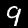
\includegraphics[width=\linewidth]{saliency/mnist_ic_saliency/original_9.png}
        \scriptsize Label 9
    \end{minipage}%

    }%
\caption[Input-gradient visualizations for ten MNIST digits]{Input-gradient visualizations of the \texttt{cnn\_maxout} IC model for ten MNIST digits, each with respect to its ground-truth label. Top: saliency maps; bottom: input images. As in the source figure, positive and negative gradient values above threshold 0.2 are colored red and blue, with ranking colorized using exponential decay.}
    \label{fig:mnist_ic_saliency}
\end{figure}


\paragraph{Accuracy trade-offs.}\label{subsec:dcinn_accuracy}

Architectural constraints can reduce expressivity~\parencite{Sill1997_MonotonicNetworks,Liu2020CertifiedMonotone}, but for the difference-of-two construction the accuracy cost is small on the convolutional base model and even negative on the \ac{mlp}, where every difference-of-two variant outperforms the unconstrained baseline; the full accuracy table across ten seeds and all eight variants is reported in Chapter~\ref{ch:experiments}.

\begin{remark}[Post-hoc and by-design, reconciled]\label{rem:posthoc_bydesign}
The MNIST study probes the same opposing-stream mechanism as post hoc decomposition: directly trained differences reach competitive accuracy and show class-dependent sensitivities on present and candidate missing strokes. Establishing faithful counterfactuals or general explanatory-role separation for these models and pretrained VGG-16/ResNet-18 split-pairs requires complete-model interventions and larger-architecture tests (Chapter~\ref{ch:conclusion}).
\end{remark}

\section{Game-Based Attribution: Modes and Technicalities}\label{sec:game_based_attribution}

The game route attributes by the per-neuron difference of players' discounted equilibrium occupation measures. It recovers gradients in the \ac{sg} (Theorem~\ref{ptnb:thm:gradient}) and the full $\alpha\beta$-\ac{lrp} family in the \ac{rg} at $\tau=1$ (Theorem~\ref{thm:lrp_recovery}). Here we collect tunable \emph{modes} and input-side \emph{technicalities}.

\subsection{Attribution Modes}\label{subsec:attribution_modes}

Chapter~\ref{ch:game_theory} varies equilibrium trajectory laws through routing and stopping temperatures $\tau,\theta$, the policy-entropy bonus, risk $\lambda\le0$, stream balance $(\alpha,\beta)$, and \ac{lrp} stabilization $\epsilon\ge0$. Section~\ref{sec:risk_aversion_regularization} gives an exact dictionary from each parameter to its backward rule. These controls yield tunable attribution maps and form the sweeps of Chapter~\ref{ch:experiments}.

Here $(\alpha,\beta)$ denotes the $\alpha\beta$-\ac{lrp} discount pair, with $\alpha-\beta=1$ and anchor $(2,1)$ weighting support against opposition; a bare $\alpha$ is this stream weight, unrelated to the backward shift $\alpha\in[0,\tfrac12]$ of Section~\ref{sec:split_attribution_concept}. Routing temperature $\tau$ recovers $\alpha\beta$-\ac{lrp} exactly only at $\tau=1$ (Theorem~\ref{thm:lrp_recovery}); its myopic application preserves the forward pass. It is distinct from the spatial transforms $\tau_t$ below.

\subsection{Technicalities}\label{subsec:technicalities}

Input-transform averaging and a detached-operator (DAVE-style) reading of the gradient decomposition improve maps without changing the game. They matter especially for \acp{vit}, whose $16\times16$ patch tokenization breaks translation equivariance and introduces grid artifacts~\parencite{Wrobel2024,Dosovitskiy2021vit}.

\paragraph{Reynolds-inspired averaging.} Following DAVE~\parencite{Wrobel2024}, compute attributions on $N$ randomly transformed inputs (small rotations, translations, horizontal flips), map them back by $\tau_t^{-1}$, and average. These spatial transforms $\tau_1,\dots,\tau_N$ are distinct from routing temperature $\tau$. Reynolds-inspired averaging can suppress transform-dependent architectural artifacts while retaining common image structure; $N$ trades computation for smoothness and is ablated in Chapter~\ref{ch:experiments}.

\paragraph{Connection to DAVE-style gradient decomposition.} The averaging pairs with a \emph{conditioned forward pass} inspired by DAVE \parencite{Wrobel2024}. Our game fixes both LayerNorm statistics, the GELU gate and the softmax row; DAVE retains linear mean-centering while fixing the normalization scale. Conservation concerns the game's propagation rule with its bias accounting. The attribution takes the transform-averaged input$\times$gradient form $\tfrac{1}{N}\sum_t \tau_t^{-1}(W_t) \odot X$, where $W_t$ is the conditioned backward signal on the $t$-th transformed input. Chapter~\ref{ch:transformers} specifies the conditioned operators used by the game-based maps.

\chapter{Experiments and Evaluation}\label{ch:experiments}

This chapter evaluates two design choices: exposing split streams to attribution and changing backward routing through game policies. The split-method and game-based campaigns examine localization, faithfulness, robustness, and numerical or computational cost. We retain their checkpoints, sample exclusions, metric conventions, and selection protocols, comparing scores within each campaign. Model-evaluation scores come from the papers; Pascal VOC uncertainty estimates and comparison statistics are recomputed locally using images as independent sampling units.

\section{Experimental Setup}\label{sec:experimental_setup}\label{sec:quantus_evaluation}

The split campaign evaluates pretrained VGG-16 and ResNet-18 on a custom 50-class ImageNet-S subset at $224\times224$ resolution. The source paper reports 50 validation images (one per class) for layer--formula selection and 566 test images. Its released loader selects locally available image--mask pairs without the game campaign's label-agreement filter; these counts alone cannot recover historical sample membership. Explanations target the predicted class, including for misclassified images; localization uses the annotated object mask. Baselines use Captum, Zennit for $\gamma$-LRP, and separate Grad-CAM++ and LayerCAM implementations. Each method retains localization-selected and Pixel-Flipping-selected configurations (full settings and results: Section~\ref{app:saliency} of the supplement).

The split tables report Pixel Flipping as score-drop AUC (PF$^{\mathrm{drop}}_5$, PF$^{\mathrm{drop}}_{20}$; $\uparrow$), perturbing 112 scalar input features per step, and Maximum Sensitivity with 25 perturbations. The revised game campaign reports remaining-logit AUC (PF$_5$, PF$_{20}$; $\downarrow$), with 1,568 scalar features per step, and sensitivity with 50 perturbations on a common 200-image test subset. Both Pixel-Flipping implementations broadcast spatial attribution over color channels, indexing the flattened $C\times H\times W$ input: $150{,}528$ features for RGB images at this resolution. Quantus measures Selectivity, Attribution Localization and Pointing Game. Both campaigns include VGG-16; their ResNet-18 and ResNet-50 scores are not interchangeable. Table abbreviations are AL (Attribution Localization), PG (Pointing Game), Sel (Selectivity), MaxS (Maximum Sensitivity), AvgS (Average Sensitivity), GCAM (Grad-CAM), GCAM++ (Grad-CAM++), LCAM (LayerCAM), IntGrad (Integrated Gradients), and SmGrad (SmoothGrad); Guided GCAM denotes Guided Grad-CAM. Dark blue shading and bold type mark the best values within each caption's comparison; n/r means unreported in the source paper, and n/a means inapplicable.

\section{Split Methods: VGG-16}\label{sec:results_vgg}

\input{figures/experiments/vgg_saliency_comparison_main}

\paragraph{Qualitative analysis.}
Figure~\ref{fig:vgg_saliency_comparison_main} compares split and baseline saliency maps at their best-performing layers. Mid-layer SplitCAM resembles earlier-layer classical $\gamma$-\ac{lrp}. Against same-layer LayerCAM, it gives more weight across object pixels while emphasizing key features, balancing interpretability and focus (low entropy). For $\alpha \ll 0.5$, SplitGrad yields less focused, finely aligned gradients following image details. We attribute this to Maxout retaining pre-activation information that ReLU discards at inactive neurons. Further examples appear in Section~\ref{app:saliency} of the supplement.

\input{tables/eval_vgg_main}

\paragraph{Quantitative analysis.}
Tables~\ref{tab:eval_vgg_main} and~\ref{tab:eval_res_main} compare selected VGG-16 and ResNet-18 configurations on five Quantus metrics: Selectivity, Attribution Localization, Pointing Game accuracy, Pixel Flipping (score-drop AUC, PF$^{\mathrm{drop}}_5$ and PF$^{\mathrm{drop}}_{20}$), and Maximum Sensitivity. \emph{Abs} indicates absolute saliency values before Quantus evaluation. Full results, explanations, layers and parameter configurations appear in Section~\ref{app:saliency} of the supplement.

The backpropagation-based methods depend strongly on layer choice (ablations: Section~\ref{app:ablation} of the supplement).

VGG-16 gains depend on metric and configuration. Table~\ref{tab:eval_vgg_main} gives SplitCAM Pointing Game $0.938$ versus Guided Backprop's $0.887$, Attribution Localization $0.651$ versus Guided Backprop's $0.632$, and Selectivity $2.727$ versus LayerCAM's $2.792$, from different SplitCAM layers. LayerCAM has the highest displayed Pixel Flipping score-drop AUCs, $0.317$ and $2.474$, versus SplitCAM's $0.300$ and $2.404$. SplitLRP has the lowest Maximum Sensitivity, $0.282$, versus Guided Backprop's $0.375$, and higher Pointing Game but lower Attribution Localization and Pixel Flipping scores than the displayed classical $\gamma$-\ac{lrp} configurations.

\section{Split Methods: ResNet-18}\label{sec:results_resnet}

\input{tables/eval_res_main}

Table~\ref{tab:eval_res_main} reports selected ResNet-18 configurations on the same five metrics, with \emph{Abs} indicating absolute saliency before evaluation (full tables: Section~\ref{app:saliency} of the supplement). SplitCAM has the lowest reported Selectivity, $3.503$, versus $3.517$ for the strongest baseline, Guided Backprop: a difference of $0.014$. SplitCAM and SplitGrad reach Pointing Game $0.972$ versus LayerCAM's $0.971$. Attribution Localization is $0.673$ for SplitCAM and $0.664$ for LayerCAM; Guided Grad-CAM leads the full comparison at $0.742$ (Table~\ref{tab:xai_eval_comprehensive_res}). Baselines retain the best Pixel Flipping and Maximum Sensitivity scores: the gains are metric-specific.

\section{Split-Method Stabilization Ablations}\label{sec:ablations}
\subsection{Backward-Pass Stabilization of the Split Methods}\label{subsec:alpha_ablation}

\input{tables/alpha_ablation_main}

Table~\ref{tab:alpha_ablation_main} varies the shift $\alpha$ for two selected SplitGrad and SplitCAM configurations on the custom ImageNet-S test split. As in Section~\ref{sec:stabilization_dc}, $\alpha = 0$ leaves the backward pass unstabilized; $\alpha = 0.5$ gives local sensitivities resembling scaled original-network gradients. Reducing $\alpha$ from $0.5$ to $0.4$ improves both configurations' Pointing Game and Attribution Localization, while SplitCAM's PF$^{\mathrm{drop}}_{20}$ falls from $1.607$ to $1.585$. SplitGrad peaks in PF$^{\mathrm{drop}}_{20}$ at $\alpha = 0.4$ and localization at $\alpha = 0.35$; SplitCAM's Pointing Game and Attribution Localization peak at $0.4$ and $0.35$, respectively. Both minimize Maximum Sensitivity at $\alpha = 0$. The sweep supports metric-dependent $\alpha$ choices; numerical stabilization and attribution-rule changes remain confounded. Section~\ref{app:ablation} of the supplement (Table~\ref{tab:alpha_comparison_by_method}) gives the full grid and compares convex with winner-takes-it-all max-pooling.

For the same SplitCAM configuration, Tables~\ref{tab:eval_vgg_main} and~\ref{tab:alpha_ablation_main} retain conflicting source values: PF$^{\mathrm{drop}}_{20}=1.590$ versus $1.585$ and MaxS$=0.456$ versus $0.457$. Resolving this discrepancy requires unavailable per-image results.

\paragraph{Forward-pass stabilization.}
Without forward stabilization (Section~\ref{sec:stabilization_dc}), late VGG-16 split activations grow to order $10^{18}$, producing errors of order $10^{9}$; SplitLRP produces nearly uniform maps. Scaling outperforms shifting on every reported metric in the two early-layer SplitLRP configurations. At later layers, shifting gives higher Attribution Localization and Pixel-Flipping score-drop AUC, scaling lowers Maximum Sensitivity, and Pointing Game depends on configuration (supplement Table~\ref{tab:lrp_scale_shift_comparison}; unstabilized and shift-stabilized SplitCAM grids: Tables~\ref{tab:alpha_comparison_none} and~\ref{tab:alpha_comparison_shift}).

\section{Game-Based Case Study}\label{sec:results_vit}\label{sec:saliency_results}\label{ptnb:sec:experiments}\label{ptnb:sec:case-study}



\paragraph{Setup.}
We evaluate \ac{rg} and \ac{sg} against standard backward baselines (Section~\ref{ptnb:app:baselines})
on VGG-16~\parencite{Simonyan2015}, ResNet-50~\parencite{He2016resnet}, and
ViT-B/16~\parencite{Dosovitskiy2021vit}, using PyTorch~\parencite{Paszke2019PyTorch} and torchvision ImageNet-1K
checkpoints~\parencite{Deng2009,Russakovsky2015ilsvrc}\footnote{Checkpoint documentation: \url{https://docs.pytorch.org/vision/stable/models.html}; the weight identifiers used here are listed in Section~\ref{app:extended_protocol}.}, on a 50-class
ImageNet-S subset~\parencite{gao2022luss} at $224{\times}224$ (50-image validation split, 565-image
test split), and on Pascal VOC 2012~\parencite{Everingham2010voc}\footnote{Release documentation: \url{https://www.robots.ox.ac.uk/~vgg/projects/pascal/VOC/voc2012/}.}. For the game campaign, the $752$ released ImageNet-S50 annotation records are filtered to $616$ whose class agrees with the official ILSVRC2012 label; one image per class is selected for validation with seed $42$, and one of the remaining $566$ test images is excluded because its object mask is outside the center crop. The explanation target is the dataset class, including on misclassified images (Section~\ref{ptnb:app:protocol}). ImageNet-S provides the pixel masks
required by the localization metrics; ImageNet boxes over-credit mass anywhere inside the box. All
metrics are computed through Quantus~\parencite{Hedstrom2023} (definitions in
Section~\ref{ptnb:app:metrics}): localization (\ac{ptnbAttrLoc}, \ac{ptnbPG}, Top-$k$ Intersection (TK);
$\uparrow$), faithfulness (Pixel Flipping area under the remaining-logit curve over the first 5\% and 20\% of flips
(PF$_5$, PF$_{20}$), \ac{ptnbSel}; $\downarrow$), robustness (Maximum Sensitivity (MaxS), Average
Sensitivity (AvgS); $\downarrow$). Baselines run in their reference implementations (lxt, zennit,
captum, pytorch-grad-cam, and the authors' code for \acs{ptnbTIBAV} and \acs{ptnbGAE}) at the authors'
settings, plus declared grids~\parencite{Achtibat2024AttnLRP,Anders2021Zennit,kokhlikyan2020captum,Gildenblat2021gradcam,Chefer2021GenericAttention,Chefer2021ICCV}. \ac{rg} analytical modes are
reported alongside each configuration: temperature $\tau$, risk aversion $\lambda$ (softmax-shift
variant $\lambda_{\mathrm{sm}}$ on \ac{vit} attention logits), \ac{lrp} stabilizer $\varepsilon$,
equivariant-Reynolds sample count $N$.

\paragraph{Protocol.}
Methods are evaluated under a two-stage protocol that treats baselines and our games alike. Stage~1
runs a grid search on the validation split (one image per class) for every method with tunable
parameters, including DAVE (Section~\ref{ptnb:app:grids}, Table~\ref{ptnb:tab:main-search-grid}; \nValGrid{}
configurations in total). Stage~2 picks, for each method, the \emph{loc} configuration with the
best localization rank-sum over $\{\text{AL}, \text{PG}, \text{TK}\}$ and, independently, the
\emph{faith} configuration with the best faithfulness rank-sum over $\{\text{PF}_5, \text{PF}_{20},
    \text{Sel}\}$, and evaluates both once on the test split, with 95\% percentile-bootstrap confidence
intervals~\parencite{Efron1993bootstrap} and Holm-corrected~\parencite{Holm1979} paired tests against the
best row of each metric (Section~\ref{ptnb:app:stats}); for \ac{rg} / \ac{rg}+Eq we additionally show
the $\alpha\beta$-\ac{lrp} anchor $(\alpha,\beta,\varepsilon,\tau){=}(2,1,0.5,1)$ as a
theorem-driven reference (Theorem~\ref{ptnb:thm:lrp-recovery}). Localization is a natural target for
modes designed to control routing focus, and object annotations provide external ground truth:
\textcite{Kohlbrenner2020} compare \ac{lrp} rule composites by the share of positive relevance inside
ground-truth bounding boxes; we use absolute attribution mass and pixel masks. The main table reports the loc row of every
method; since mask agreement is not faithfulness, the faith rows of all methods are reported in
Section~\ref{ptnb:app:results}.

\begin{table}[H]
    \centering
    \caption[ViT-B/16 on the ImageNet-S test split]{ViT-B/16 on the ImageNet-S test split ($n{=}565$; MaxS/AvgS on a fixed random subset of
    200 test images). \textbf{Bold}, dark shading: best in column; $^{\approx}$, light shading: not
    significantly different from the best (paired bootstrap / McNemar, Holm-corrected, $p\ge0.05$);
    small numbers: 95\% percentile-bootstrap confidence intervals over test images
    (Section~\ref{ptnb:app:stats}). One row per method, selected on the validation split by the
    localization rank-sum (faithfulness-selected rows and further baselines:
    Section~\ref{ptnb:app:results}); the RG anchor is the exact $\alpha\beta$-\ac{lrp} representation
    (Theorem~\ref{ptnb:thm:lrp-recovery}). $t$/img: seconds per image on one GPU. Config: SmoothGrad
    averages $N$ samples at noise level $\sigma$ relative to the input range; LRP-$\gamma$ has
    stabilizer $\varepsilon$ and positive-weight boost $\gamma$; AttnLRP has layer-type parameters
    $\gamma_{\mathrm{conv}}, \gamma_{\mathrm{lin}}, \varepsilon_{\mathrm{attn}}$; KernelSHAP draws $N$
    samples for $M$ superpixels; \ac{rg} modes as in Table~\ref{ptnb:tab:modes}.\PrelimTag}
    \label{ptnb:tab:eval-vit}\label{tab:eval-vit}
\TableContent{
    \scriptsize
    \resizebox{\textwidth}{!}{\input{tables/ptnb_v2/generated/main_vit_tabular}}
}%
\end{table}

\paragraph{ViT-B/16 (Table~\ref{ptnb:tab:eval-vit}).}
Under the localization-selected protocol, the \ac{rg} family beats every baseline on attribution
localization, including the prior transformer-specific backward methods
AttnLRP~\parencite{Achtibat2024AttnLRP}, our DAVE implementation~\parencite{Wrobel2024} (Section~\ref{ptnb:app:baselines}),
\ac{ptnbTIBAV}~\parencite{Chefer2021GenericAttention} and \ac{ptnbGAE}~\parencite{Chefer2021ICCV}: the selected mode
reaches AL \vitRGlocAL{} against \vitBestBaseAL{} for the best baseline (\vitBestBaseALname), and
\ac{rg}+Eq \vitRGEqlocAL{}, both significantly ahead of every baseline row after Holm correction.
\ac{rg}+Eq also has the highest observed TK (\vitRGEqlocTK{}), but the Holm-corrected tests do not detect a difference from \vitBestBaseTKname{}
at \vitBestBaseTK{} or LRP-$\gamma$ at $0.816$. The pointing game is led by \vitBestBasePGname{} (\vitBestBasePG{}), whose
maps are constant on superpixels: a hit needs only one pixel of the maximal region inside the mask.
Scoring a single pixel drawn from that region instead, KernelSHAP falls below \ac{rg}+Eq, which is
then not significantly below the best baseline (LRP-$\gamma$; Section~\ref{ptnb:app:pg-granularity}).
Among the localization-selected rows, faithfulness favors the \ac{lrp} rules: AttnLRP is best on PF$_5$ and PF$_{20}$ and LRP-$\gamma$ on
Sel (PF$_{20}$ \vitBestBasePFtwenty{} versus \vitRGlocPFtwenty{} for \ac{rg}), and the
faithfulness-selected \ac{rg} row narrows but does not close the gap (PF$_{20}$
\vitRGfaithPFtwenty{}). Across both selection objectives, faithfulness-selected AttnLRP has the lowest PF$_5$, PF$_{20}$ and Selectivity, at $7.64$, $6.12$ and $4.441$, respectively. The two anchors are the most robust rows (MaxS \vitRGanchorMaxS{} and
\vitRGEqanchorMaxS{} versus \vitBestBaseMaxS{} for \vitBestBaseMaxSname{}), whereas the
localization-selected mode reaches MaxS \vitRGlocMaxS{}: sharper routing trades robustness and
faithfulness for localization. \ac{ptnbADF} adds modest overhead (\ac{rg}: \vitRGlocTime\,s vs.\
\vitRGanchorTime\,s base), still below sampling baselines like SmoothGrad or IntGrad; Reynolds
averaging is the only expensive variant (\vitRGEqTime\,s), exceeding even the perturbation method
KernelSHAP (\vitSHAPTime\,s).

\paragraph{Higher $\tau$ spreads attribution into context.}
Localization-optimal modes concentrate mass on the few patches aligning with the mask. Increasing $\tau$ spreads equilibrium routing over more predecessors: the displayed examples retain object focus while extending attribution into context, without establishing which contextual features the model uses. Around the selected ViT-B/16 setting, AL decreases monotonically from $0.723$ at $\tau{=}0.3$ to $0.461$ at $\tau{=}1$; faithfulness is non-monotonic. High $\tau$ shows how localization scores favor concentrated maps within the same game. User-perceived informativeness remains untested.

\paragraph{Cross-dataset transfer (Pascal VOC).}
A natural worry with validation-tuned modes is that the chosen $\tau$, $\lambda_{\mathrm{sm}}$ and
$\sigma^2$ are overfitted to the ImageNet-S 50-class subset. We test transfer on a per-image
disjoint split of Pascal VOC 2012 trainval ($2{,}743$ test (image, foreground-class) samples with
pixel-accurate segmentation masks): \ac{rg} and \ac{rg}+Eq use the \emph{same} mode parameters as
Table~\ref{ptnb:tab:eval-vit} without any VOC-side re-tuning, while every baseline gets a fresh
per-method validation grid on the new pool. This tests the portability of the selected parameters
across these datasets for the same pretrained model, without identifying whether the underlying
structure is model-specific or dataset-specific. The localization lead carries over (AL
\vocRGlocAL{} for \ac{rg} and \vocRGEqlocAL{} for \ac{rg}+Eq versus \vocBestBaseAL{} for
\vocBestBaseALname{}, both significant against every baseline row), while TK and PG are led by
\ac{ptnbTIBAV} and the perturbation methods, and faithfulness by the \ac{lrp} rules
(Section~\ref{ptnb:app:voc-cross-data}).

\paragraph{VGG-16 and ResNet-50 (Section~\ref{ptnb:app:results}).}
On CNNs, where \ac{lrp}-type rules are strong, localization-selected \ac{rg} leads AL within that selection: clearly on VGG-16 (\vggRGlocAL{} versus \vggBestBaseAL{} for \vggBestBaseALname{}) and narrowly on ResNet-50 (\resRGlocAL{} versus \resBestBaseAL{} for \resBestBaseALname{}). The ResNet-50 difference is not Holm-significant (adjusted $p=0.420$), so its numerical lead does not establish superiority. Across both objectives, VGG-16's strongest baseline AL is faithfulness-selected LRP-$\varepsilon$ at $0.639$, below \ac{rg}'s \vggRGlocAL{}. Pixel Flipping favors LRP-$\varepsilon$ for VGG-16 PF$_5$ ($12.43$), LRP-$\gamma$ for VGG-16 PF$_{20}$ ($7.89$ versus LRP-$\varepsilon$'s $8.17$), and LRP-$\gamma$ for both ResNet-50 metrics; \ac{cam} and perturbation methods lead TK and PG. VGG-16's risk-averse \ac{sg} is most robust (MaxS \vggSGlocMaxS{} versus \vggBestBaseMaxS{} for \vggBestBaseMaxSname{}).

\subsection{Game-Method Ablations}\label{subsec:mode_ablation}

Section~\ref{ptnb:app:abl-one-factor} varies one mode around each validation-selected configuration on 565 test images; these diagnostics do not affect selection. Section~\ref{ptnb:app:pg-granularity} controls Pointing Game for map granularity, and Section~\ref{ptnb:app:abl-gradient-fallback} compares composite Value-routing attention with a gradient fallback. The analyses reveal trade-offs among mask agreement, perturbation faithfulness and robustness.

\chapter{The Trajectory Distribution View}\label{ch:trajectory}

Chapter~\ref{ch:saliency} turns internal signals and backward routing choices into attribution maps; Chapter~\ref{ch:experiments} evaluates them. Their use in interventions also requires examining the underlying calculation. The equilibrium policies of Chapter~\ref{ch:game_theory} induce backward-trajectory distributions, enabling comparison before projection onto input pixels. We study their Hellinger distance, its exact per-input-state disagreement map, and complete versus survival-conditioned laws. Spectral analysis diagnoses amplification and target discrimination through the attribution redistribution operator's singular spectrum at a fixed input~\parencite{Maess2026Spectral}; our experiments compare normalized routing under input noise and parameter randomization.

\section{Comparison with Normalized Relevance Measures}\label{sec:nrm_comparison}

The \ac{nrm} framework of \textcite{Xiong2026nrm}, by Ping Xiong, Thomas Schnake, Grégoire Montavon, Klaus-Robert Müller, and Shinichi Nakajima, studies backward calculations through a normalized signed measure on complete neuron walks. Summing walk relevance through selected neurons or concepts gives their relevance; conditional relevance divides joint by nonzero marginal relevance. With suitable normalized propagation rules, this covers ordinary \ac{lrp}, concept relevance, and Concept Relevance Propagation (CRP)~\parencite{Achtibat2023CRP}. Their CRP quantity is joint relevance of an input neuron, intermediate concept neuron, and target output, without an automatic conditional-probability interpretation.

Both views retain network paths before forming attribution maps; their factorization supports sum-product computation and queries across layers. In \ac{nrm}, individual walk relevance may be negative despite unit total. Our game policies define a non-negative probability law $\Pi$ on the expanded graph, including player labels and termination. Signed differences of its discounted occupation measures recover gradients and relevance scores (Chapter~\ref{ch:game_theory}), generally distinct from unweighted marginals. Player expansion thus separates trajectory probability from contribution sign and scale, without identifying $\Pi$ with a given \ac{nrm} measure.

The \ac{nrm} construction normalizes propagation columns under positive-sum assumptions; identifying it with globally normalized original walk relevance additionally requires the constant-sum conditions of \textcite[Section~3.5]{Xiong2026nrm}. Our transitions remain normalized; discounts retain scale, with explicit bias and stabilizer absorption. Hellinger distance applies directly to these probability laws, but generally not to signed relevance measures. Conditioning $\Pi$ on a concept requires positive probability; signed relevance can instead vanish by cancellation.

Symbolic XAI scores logical feature queries by selecting signed terms from a multi-order prediction decomposition~\parencite{Schnake2025SymbolicXAI}. SemanticLens combines component attributions and semantic embeddings to audit expected and spurious visual concepts~\parencite{Dreyer2025SemanticLens}. These address feature relationships and human interpretation; trajectory probabilities describe normalized routing. We propose querying game trajectories through concepts, retaining attribution signs and discounts, and comparing their laws across inputs or models. Equivalence with a particular \ac{nrm}/CRP construction remains unproved and would require matching propagation rules, normalization, and absorption conventions.

\section{Trajectory Sanity Check}\label{ptnb:sec:hellinger-sanity}\label{ptnb:sec:hellinger}

The cascading-randomization sanity check of~\textcite{Adebayo2018sanity} tests explanations' dependence on learned parameters by comparing pixel-space maps. Here we examine normalized backward routing: a trajectory distribution $\Pi$ whose model-dependent signed discounted occupation projection recovers attribution.
The \textbf{Hellinger distance}~\parencite{Hellinger1909} $\mathrm{H}(\Pi_A, \Pi_B) = (1 -
    \mathrm{BC})^{1/2}$, with Bhattacharyya coefficient~\parencite{Bhattacharyya1943} $\mathrm{BC} =
    \sum_\zeta \sqrt{\Pi_A(\zeta)\,\Pi_B(\zeta)}$, directly compares routing. We test whether parameter randomization moves $\Pi$ even when attribution maps remain stable. The metric satisfies $\mathrm{H}=0$ iff $\Pi_A = \Pi_B$ and $\mathrm{H}=1$ iff their supports are disjoint. It remains finite when routes open or close, unlike KL-type divergences. For layered Markov laws on the same graph, BC factorizes: one backward pass computes $\mathrm{H}$ exactly in edge-linear time, and $\mathrm{H}^2$ decomposes into per-input-state contributions (Section~\ref{ptnb:app:path-divergence}).

\subsection{Trajectories change, maps need not}\label{ptnb:sec:hellinger-cascading}

\begin{figure}[t]
    \centering
    \input{figures/ptnb_v2/plots/sanity_check/hellinger_live_plots.inc.tex}
    \caption[Hellinger trajectory distance under parameter randomization]{Hellinger trajectory distance under cascading parameter
    randomization~\parencite{Adebayo2018sanity}. Hellinger distance $\mathrm{H}$ (vertical axis, from
    $0.7$) against the number of cascadingly re-initialized layers, output to input (horizontal axis;
    $\mathrm{H}=0$ before the first layer is randomized). Solid: plain $\mathrm{H}$; dotted:
    $\mathrm{H}_{\mathrm{surv}}$, conditioned on survival to an ordinary input-layer state. Thin
    horizontal reference lines mark the double-random baseline values from
    Table~\ref{ptnb:tab:double-random-hellinger} (solid: plain $\mathrm{H}$; dotted:
    $\mathrm{H}_{\mathrm{surv}}$), in the color of the corresponding game.}
    \label{ptnb:fig:hellinger-sanity}
\end{figure}

Under cascading randomization (layers cumulatively re-initialized output$\to$input), \ac{sg} and \ac{rg} diverge from the first randomized layer and plateau near the double-random reference (Table~\ref{ptnb:tab:double-random-hellinger}, Figure~\ref{ptnb:fig:hellinger-sanity}). This reference lies below $\mathrm{H}=1$ because models randomized over the tested layers still share short trajectories: both may stop at structurally dead neurons and enter the common cemetery. Such paths coincide more readily than full input-reaching trajectories. Conditioning on survival removes shared cemetery mass, yielding $\mathrm{H}_{\mathrm{surv}} \approx 1$. Trajectory and map readouts have weak observed per-image rank association (Spearman $|\rho|\le \perImageCrossMax$ between $\mathrm{H}$ and pixel-level Gradient or $\alpha\beta$-\ac{lrp} similarity): similar maps need not imply similar calculations. Section~\ref{ptnb:app:sanity-check} details per-game values, conditioning, the floor mechanism, and per-image analysis.

\paragraph{What the map hides.}\label{ptnb:sec:pixel-sanity}
Map-level checks under parameter randomization reproduce~\textcite{Adebayo2018sanity} and \textcite{sixt2020whenexplanationslie}: some methods retain structure at the cascade endpoint. On ViT-B/16, the \ac{rg} anchor retains Spearman $|\rho| = \sanityVitRGanchorRho$, highest among all methods, and HOG $r = \sanityVitRGanchorHOG$; VGG-16 LRP-$\varepsilon$ retains $\sanityVggLRPepsRho$ and $\sanityVggLRPepsHOG$ (Table~\ref{tab:sanity-check}). Localization-selected \ac{rg} modes are slightly more model sensitive than the anchor on all three models. \ch{In Figure~\ref{ptnb:fig:hellinger-sanity}, $\mathrm{H}$ reaches the double-random reference while maps retain structure. The map-level failure remains; $\mathrm{H}$ detects routing changes obscured by the map. Since discounted occupation projections also vary across models, this discrepancy does not isolate loss under a fixed projection.}
\section{Hellinger Distance and Disagreement Map}\label{ptnb:app:path-divergence}

We compare two layered Markov processes on a common state graph and seek both a scalar divergence
of the trajectory distributions and an exact per-pixel decomposition of this divergence at the
input layer.  We use the squared Hellinger distance because the geometric mean $\sqrt{PQ}$
preserves the multiplicative structure of Markov trajectory distributions and yields an exact
linear-time dynamic program.  Unlike Jeffreys divergence, it remains finite under support mismatch;
unlike Jensen--Shannon, it admits an exact recursion on the layered graph.  Later, we decompose the
squared Hellinger distance as a sum of non-negative per-pixel contributions over all input-layer
states, giving a disagreement map at the input layer (Theorem~\ref{ptnb:thm:per-pixel}).

The formal foundations and proofs are given in companion Chapter~\ref{app:supp_trajectory}.
We compare two processes on a common finite layered state graph with a shared deterministic
starting state $s_0$. At layer $l$, $\mathcal S^{(l)}_+=\mathcal S^{(l)}\cup\{\dagger\}$
contains the ordinary states and an absorbing cemetery state; $T_M^{(l)}$ is the transition
kernel from layer $l$ to $l-1$, and $m_M^{(l)}(s)$ is the marginal probability of visiting $s$.
The full trajectory law is $\Pi_M=\Pi_M^{(0)}$.
For the \ac{rg}, full-law diagnostics retain the gate, branch, and routing substeps; only
ordinary surviving paths admit exact act-only elimination
(Remark~\ref{ptnb:rem:rg-natural-equivalence}).

\subsection{Bhattacharyya Coefficient and the Geometric-Mean Kernel}\label{ptnb:sec:lmp-bc}

\paragraph{Definitions.}
For two probability distributions $P, Q$ on a common finite set, the \emph{Bhattacharyya
coefficient} is the geometric overlap
\begin{align}\label{ptnb:eq:bc-def}
    \mathrm{BC}(P, Q) \;\coloneqq\; \sum_{y} \sqrt{P(y)\, Q(y)} \;\in\; [0, 1],
\end{align}
and the \emph{squared Hellinger distance} is
\begin{align}\label{ptnb:eq:hellinger-def}
    \mathrm{H}^2(P, Q) \;\coloneqq\; \tfrac{1}{2} \sum_y \bigl(\sqrt{P(y)} - \sqrt{Q(y)}\bigr)^2 \;=\;
    1 - \mathrm{BC}(P, Q) \;\in\; [0, 1].
\end{align}
The Hellinger distance $\mathrm{H}(P,Q) = \sqrt{1 - \mathrm{BC}(P,Q)}$ is a true metric: $0 \leq
    \mathrm{H} \leq 1$, with $\mathrm{H} = 0$ iff $P = Q$ and $\mathrm{H} = 1$ iff $P$ and $Q$ have
disjoint supports.  Crucially, $\sqrt{0 \cdot Q(y)} = 0$, so mismatched supports cause no
infinity---only a smaller overlap.

\paragraph{Geometric-mean kernel.}
For each layer $l \geq 1$ and pair of states $(s, s') \in \mathcal{S}^{(l)}_+ \times
    \mathcal{S}^{(l-1)}_+$, define the \emph{geometric-mean kernel}
\begin{align}\label{ptnb:eq:geom-kernel}
    \widetilde{T}^{(l)}(s, s') \;\coloneqq\; \sqrt{T^{(l)}_A(s \to s')\; T^{(l)}_B(s \to s')}.
\end{align}
This kernel is non-negative but in general sub-stochastic.  Its row sum
\begin{align}\label{ptnb:eq:geom-rowsum}
    \widetilde{R}^{(l)}(s) \;\coloneqq\; \sum_{s' \in \mathcal{S}^{(l-1)}_+} \widetilde{T}^{(l)}(s, s')
\end{align}
satisfies $0 \leq \widetilde{R}^{(l)}(s) \leq 1$ by Cauchy--Schwarz, with equality iff $T^{(l)}_A(s
    \to \cdot) = T^{(l)}_B(s \to \cdot)$.  Cemetery handling is automatic: $T^{(l)}_A(\dagger \to
    \dagger) = T^{(l)}_B(\dagger \to \dagger) = 1$, so $\widetilde{T}^{(l)}(\dagger, \dagger) = 1$ and
$\widetilde{R}^{(l)}(\dagger) = 1$.

\subsection{Hellinger backward pass}\label{ptnb:sec:lmp-hellinger-backward}

The chain rule (Lemma~\ref{ptnb:lem:bc-chain-rule}) yields a backward DP that propagates the per-state
cumulative $\widetilde{T}$-mass $g^{(l)}(s)$ from the start state $s_0$ down through the layers.
The prefix Bhattacharyya coefficient at each layer is the row sum $\mathrm{BC}^{(l)} = \sum_{s}
    g^{(l)}(s)$, the prefix Hellinger distance is $\mathrm{H}^{(l)} = \sqrt{1 - \mathrm{BC}^{(l)}}$,
and the per-terminal-state disagreement map is read off at $l = 0$ from~\eqref{ptnb:eq:per-pixel-h2}.
The map is defined on the full terminal set $\mathcal{S}^{(0)}_+ = \mathcal{S}^{(0)} \cup
    \{\dagger\}$; the visualized pixel attribution map is its restriction to ordinary pixels
$\mathcal{S}^{(0)}$, and its sum is therefore $\mathrm{H}^2_{\mathrm{ord}} = \mathrm{H}^2 -
    \mathrm{H}^2(\dagger)$, not the full $\mathrm{H}^2$ (Theorem~\ref{ptnb:thm:per-pixel}(iii)).

\begin{algorithm}[H]
    \caption{Hellinger backward pass (with per-terminal-state disagreement map)}
    \label{ptnb:alg:hellinger}\label{ptnb:alg:hellinger-backward}
    Initialize the occupation marginals $m_M^{(L)}$ and overlap mass $g^{(L)}$ at the target output.\;
For $l=L,L-1,\ldots,1$, propagate each model's marginals with its kernel and propagate overlap by
$g^{(l-1)}(s')=\sum_s g^{(l)}(s)\sqrt{T_A^{(l)}(s,s')T_B^{(l)}(s,s')}$.\;
At each layer compute $\mathrm{BC}^{(l)}=\sum_s g^{(l)}(s)$ and
$\mathrm{H}^{(l)}=\sqrt{1-\mathrm{BC}^{(l)}}$.\;
At every terminal state return
$\mathrm{H}^2(s)=\tfrac12(m_A^{(0)}(s)+m_B^{(0)}(s))-g^{(0)}(s)$.
The pixel disagreement map restricts this output to ordinary input states.

\end{algorithm}

\subsection{Per-Pixel Disagreement Map}\label{ptnb:sec:lmp-disagreement}

The squared Hellinger distance $\mathrm{H}^2$ admits an exact non-negative decomposition over
input-layer states: each input pixel carries a calibrated share of the total trajectory
disagreement (Theorem~\ref{ptnb:thm:per-pixel}), giving a disagreement \emph{map} that is itself an
attribution of the trajectory mismatch back to the input. The conditioned-on-survival variant
removes the cemetery contribution that otherwise bounds plain $\mathrm{H}$ from below on randomized
models.

\subsubsection{Per-Pixel Decomposition: The Disagreement Map}\label{ptnb:sec:lmp-per-pixel}

The squared Hellinger distance at layer~$0$ decomposes exactly over terminal pixels.

\begin{theoremenv}[Per-pixel decomposition, \LeanResult{ptnb:thm:per-pixel}]\label{ptnb:thm:per-pixel}
Let $\mathrm{H}^2 \coloneqq \mathrm{H}^2\!\bigl(\Pi^{(0)}_A,\, \Pi^{(0)}_B\bigr)$.  For $s \in
    \mathcal{S}^{(0)}_+$, define
\begin{align}\label{ptnb:eq:per-pixel-h2}
    \mathrm{H}^2(s) \;\coloneqq\; \tfrac{1}{2}\bigl(m^{(0)}_A(s) + m^{(0)}_B(s)\bigr) \;-\; g^{(0)}(s),
\end{align}
where $g^{(0)}(s)$ is the cumulative $\widetilde{T}$-mass at $s$.  Then:
\begin{enumerate}
    \item[(i)] $\mathrm{H}^2(s) \geq 0$ for every $s \in \mathcal{S}^{(0)}_+$.
    \item[(ii)]
        \begin{align}\label{ptnb:eq:per-pixel-sum}
            \mathrm{H}^2 \;=\; \sum_{s \in \mathcal{S}^{(0)}_+} \mathrm{H}^2(s).
        \end{align}
    \item[(iii)]
        \begin{align}\label{ptnb:eq:ordinary-h2}
            \mathrm{H}^2_{\mathrm{ord}} \;\coloneqq\; \sum_{s \in \mathcal{S}^{(0)}} \mathrm{H}^2(s) \;=\;
            \mathrm{H}^2 - \mathrm{H}^2(\dagger)
        \end{align}
\end{enumerate}\end{theoremenv}

Proofs of the backward pass and the decomposition are given in companion Chapter~\ref{app:supp_trajectory}.

\paragraph{The disagreement map.}
Theorem~\ref{ptnb:thm:per-pixel} defines $\mathrm{H}^2(\cdot)$ on the full terminal set
$\mathcal{S}^{(0)}_+ = \mathcal{S}^{(0)} \cup \{\dagger\}$: this is the \emph{full terminal-state
decomposition}, with $\sum_{s \in \mathcal{S}^{(0)}_+} \mathrm{H}^2(s) = \mathrm{H}^2_{(0)}$, and
the cemetery contribution $\mathrm{H}^2(\dagger)$ is part of it. The \emph{Hellinger disagreement
map} is the ordinary-pixel restriction $s \mapsto \mathrm{H}^2(s)$ on $\mathcal{S}^{(0)}$, which is
the quantity we visualize. It is non-negative, sums to $\mathrm{H}^2_{\mathrm{ord}}$ over ordinary
pixels, and is computed from $g^{(0)}, m_A^{(0)}, m_B^{(0)}$.  The quantity
$\mathrm{H}^2_{\mathrm{ord}}$ is an unnormalized ordinary-state subsum; the conditioned-on-survival
Hellinger distance that normalizes it is introduced below. Recall from Section~\ref{ptnb:sec:games-fit}
that layer-$0$ ordinary states of the two games are \emph{tagged} pixel pairs $s^{(0)}_{j,\pm}$,
tagged by the player $q$ for the \ac{sg} and by the stream sign $\kappa$ for the \ac{rg}; the
per-pixel attribution displayed in figures aggregates the two tags,
\begin{align}
    \mathrm{H}^2_{\mathrm{pixel}}(j) \;=\; \mathrm{H}^2\bigl(s^{(0)}_{j,+}\bigr) +
    \mathrm{H}^2\bigl(s^{(0)}_{j,-}\bigr),
\end{align}
which remains non-negative and sums to $\mathrm{H}^2_{\mathrm{ord}}$ over pixels.  By the
Cauchy--Schwarz step in the proof of Theorem~\ref{ptnb:thm:per-pixel}(i), $g^{(0)}(s) \leq
    \sqrt{m^{(0)}_A(s)\,m^{(0)}_B(s)}$, so $\mathrm{H}^2(s)$ is bounded below by the marginal surrogate
$\tfrac{1}{2}\bigl(m^{(0)}_A(s) + m^{(0)}_B(s)\bigr) - \sqrt{m^{(0)}_A(s)\,m^{(0)}_B(s)}$, the
per-pixel squared Hellinger distance between the layer-0 marginal occupations; the trajectory map
is strictly larger whenever the conditional distributions of trajectories reaching pixel~$s$ differ
between models.

\subsubsection{Conditioning on Survival to the Ordinary Input
Layer}\label{ptnb:sec:lmp-conditioned-survival}

When the cemetery absorbs a large fraction of trajectory mass, the total Hellinger distance mixes
two effects: disagreement about \emph{whether} a trajectory survives and disagreement about
\emph{where surviving trajectories go}.  To isolate the second effect, we condition each model's
trajectory law on the event that the trajectory reaches an ordinary input-layer state.  The
resulting scalar compares the two \emph{surviving} trajectory distributions directly and removes
the common cemetery floor.  Because survival to the input layer factorizes along the layered graph,
this conditioning remains Markov and is implemented by a per-state Doob $h$-transform (with $h =
    \psi_M$, the remaining survival probability).

Let $\mathsf{Surv}$ denote this event and assume that both survival masses are positive. With
\[
 Z_M=\mathbb P_M(\mathsf{Surv})
     =\sum_{s\in\mathcal S^{(0)}}m_M^{(0)}(s)>0,
 \qquad
 \mathrm{BC}_{\mathrm{ord}}^{(0)}=\sum_{s\in\mathcal S^{(0)}}g^{(0)}(s),
\]
the conditioned-survival Hellinger distance is
\[
 \mathrm H_{\mathrm{surv}}^2
 =\mathrm H^2\!\bigl(\Pi_A(\,\cdot\mid\mathsf{Surv}),
                         \Pi_B(\,\cdot\mid\mathsf{Surv})\bigr)
 =1-\frac{\mathrm{BC}_{\mathrm{ord}}^{(0)}}{\sqrt{Z_A Z_B}}.
\]
Theorem~\ref{ptnb:thm:conditioned-survival} gives the conditioned kernels and the proof;
Equation~\eqref{ptnb:eq:conditioned-per-pixel-h2} gives the corresponding non-negative map.
Post-hoc normalization becomes numerically infeasible for deep networks when either
survival probability gets too small; the conditioned-kernel computation avoids this final division.

\subsection{Experiments}\label{ptnb:sec:lmp-experiments}

With the model fixed, we test sensitivity to input perturbations and separation among ImageNet-S classes and from random noise. We use the Stopping-Game kernel~\eqref{ptnb:eq:adf-T} without risk aversion ($\lambda = 0$; ``ADF'' in code) and Routing-Game kernel~\eqref{ptnb:eq:rg-T-act} at $\tau = 1$. The diagnostic \ac{rg} omits the bias action and renormalizes the remaining branches, so it may differ from the bias-inclusive attribution game.

\subsubsection{Input-Noise Sensitivity}\label{ptnb:sec:input-noise-hellinger}

For each architecture and $\sigma \in \{0.005,\allowbreak 0.01,\allowbreak 0.02,\allowbreak 0.03,
    \allowbreak 0.05,\allowbreak 0.1,\allowbreak 0.2,\allowbreak 0.3,\allowbreak 0.5\}$, we draw one standard-Gaussian tensor $\eta$ per image and compute $\mathrm{H}(\Pi_A(x), \Pi_A(x + \sigma\eta))$ for both kernels, targeting the clean input's argmax. Mean $\mathrm{H}$ and $\mathrm{H}_{\mathrm{surv}}$ increase with $\sigma$ for both games on all three architectures (Figure~\ref{ptnb:fig:hellinger-input-noise}). They coincide for VGG-16 \ac{rg}, whose kernel never routes to dead-neuron states. ResNet-50 and ViT-B/16 skip connections reach such states; ViT-B/16's GELU gate also sends some trajectories to the cemetery at every state. Generalised Explanation Faithfulness (GEF) correlates explanation and model-output distortion along perturbation paths~\parencite{Hedstrom2025GEF}, anchoring explanation changes to model responses. Our Hellinger curves measure routing sensitivity, without establishing this alignment or explanation faithfulness.

\begin{figure}[H]
    \centering
    \input{figures/ptnb_v2/plots/hellinger_input_noise/hellinger_input_noise_plots.inc.tex}
    \caption[Input-noise Hellinger trajectory distance]{Input-noise Hellinger trajectory distance. Solid: plain $\mathrm{H}$; dotted:
    $\mathrm{H}_{\mathrm{surv}}$, conditioned on survival to an ordinary input-layer state. $x$-axis is
    log-scale input-noise $\sigma$; same $(A,A)$ model on both sides, only the input differs.}
    \label{ptnb:fig:hellinger-input-noise}
\end{figure}

\subsubsection{Class Separability and Reference Baselines}\label{ptnb:sec:input-noise-baselines}

Class separation depends on architecture and kernel (Table~\ref{ptnb:tab:hellinger-input-random}):
\begin{itemize}
    \item On \textbf{VGG-16}, \ac{sg} gives clean-intraclass $\mathrm{H}=0.513$ below clean-interclass $\mathrm{H}=0.607$. \ac{rg} saturates at $\mathrm{H}=1$ throughout, resolving no class structure.
    \item On \textbf{ResNet-50}, \ac{rg} separates clean-intraclass $\mathrm{H}=0.786$ from clean-interclass $\mathrm{H}=0.902$; \ac{sg} does not (intraclass $0.272$ vs.\ interclass $0.268$).
    \item On \textbf{ViT-B/16}, \ac{rg} gives intraclass $0.789$ vs.\ interclass $0.882$; the \ac{sg} gap ($0.422 \pm 0.023$ vs.\ $0.435 \pm 0.017$) is smaller than the spread over pairs and does not separate classes.
\end{itemize}
Random-vs-random is lowest in every nonconstant column. Clean-vs-random is highest in each plain-$\mathrm{H}$ column except ResNet-50 \ac{sg} ($0.269$ vs.\ intraclass $0.272$) and saturated VGG-16 \ac{rg}, consistent with different routing for Gaussian and in-distribution inputs. Conditioned $\mathrm{H}_{\mathrm{surv}}$ is at least $0.99$ throughout VGG-16, ResNet-50, and ViT-B/16 \ac{rg}, providing no class-separability signal. ViT-B/16 \ac{sg} separates random-vs-random ($0.852$) from clean rows ($0.957$--$0.968$), but neither intraclass from interclass ($0.963$ vs.\ $0.968$) nor clean-vs-random ($0.957$) from clean pairs.

\begin{table}[H]
\TableContent{
    \centering\small
    \setlength{\tabcolsep}{4pt}
    \input{tables/ptnb_v2/generated/input_baseline_tabular}
    }%
\caption[Reference baselines for the input-noise sweep]{Reference baselines for the input-noise sweep, averaged over $R$ pairs drawn from the
    $565$-image ImageNet-S test split (clean rows: $R=200$ sampled pairs; clean-vs-random: $R=565$
    images paired with a fresh Gaussian each; random-vs-random: $R=200$ Gaussian pairs); entries are
    mean $\pm$ standard deviation over pairs. \textbf{clean-intraclass}: $\mathrm{H}(\Pi_A(x_1),
        \Pi_A(x_2))$ with $x_1, x_2$ from the same ground-truth class; \textbf{clean-interclass}: same,
    with distinct classes; \textbf{clean-vs-random}: one side clean, other Gaussian;
    \textbf{random-vs-random}: both sides Gaussian.}
    \label{ptnb:tab:hellinger-input-random}
\end{table}
\par\medskip
\section{Randomization Sanity Checks}\label{ptnb:app:sanity-check}\label{subsec:hellinger_randomization}

This section supports the cascading-randomization experiments of Section~\ref{ptnb:sec:hellinger-sanity}: \S\ref{ptnb:sec:lmp-randomization} extends the protocol of~\textcite{Adebayo2018sanity} to trajectory Hellinger diagnostics (Section~\ref{ptnb:app:path-divergence}); \S\ref{ptnb:app:sanity-heatmap} tests main-paper attribution maps; \S\ref{ptnb:sec:lmp-rand-double-random} gives the double-random reference; and \S\ref{ptnb:sec:per-image-orthogonality} compares trajectory and map diagnostics per image.

\subsection{Cascading Randomization in Trajectory Space}\label{ptnb:sec:lmp-randomization}

Replacing a weight matrix in the randomization test of~\textcite{Adebayo2018sanity} yields two kernels on the same graph; the Hellinger pass of Section~\ref{ptnb:app:path-divergence} quantifies their trajectory-space change. With its geometric-mean kernel $\widetilde{T}^{(l)}$ and overlap mass $g^{(l)}(s)$, $\mathrm{BC}^{(l)} = \sum_{s \in \mathcal{S}^{(l)}_+} g^{(l)}(s)$; $\mathrm{BC}^{(l)}_{\mathrm{ord}}$ restricts this sum to ordinary states $s \in \mathcal{S}^{(l)}$.

The Stopping-Game contraction bound assumes a conditional alive probability bounded
away from one; the Routing-Game bound assumes a uniform row-overlap bound strictly below one.
The precise hypotheses and proofs are in Theorems~\ref{ptnb:thm:rand-adf}
and~\ref{ptnb:thm:rand-routing}; the cemetery-floor analysis is in
Remark~\ref{ptnb:rem:adf-cemetery-floor}.

The discounted occupation measures at the input layer recover gradient and $\alpha\beta$-\ac{lrp} maps (Theorems~\ref{ptnb:thm:deriv-occ} and~\ref{ptnb:thm:ab-recovery}). The undiscounted endpoint marginal $m^{(0)}_M$ is generally different: Hellinger compares the trajectory routing laws and does not include the path discounts. Under their respective contraction hypotheses, Theorems~\ref{ptnb:thm:rand-adf}--\ref{ptnb:thm:rand-routing} show that $\Pi_M$ changes drastically under randomization, while Table~\ref{tab:sanity-check} shows that the resulting attribution maps can remain similar. \ch{The two
diagnostics therefore detect different aspects of parameter sensitivity: the map-level test
of~\textcite{Adebayo2018sanity} asks whether the explanation delivered to the user depends on the
learned parameters, the trajectory-level test whether its normalized routing does. A map can fail
the first while its routing passes the second; this discrepancy does not isolate a fixed projection
loss, since the discounts can also change across models, and it does not make such a
map adequate for model debugging~\parencite{Adebayo2018sanity,sixt2020whenexplanationslie}.}

\subsection{Heatmap similarity at the cascade endpoint}\label{ptnb:app:sanity-heatmap}

We apply the cascading randomization test of \textcite{Adebayo2018sanity} to Table~\ref{tab:sanity-check}'s attribution methods. Starting pretrained, we cumulatively re-initialize convolutional and linear layers output-to-input: weights Kaiming normal~\parencite{He2015delving}, biases $\mathcal{N}(0, 0.01^2)$. BatchNorm (ResNet-50), LayerNorm, positional embeddings, and class token (ViT-B/16) retain pretrained values. The ViT attribution cascade randomizes decomposed query/key/value projections; the Hellinger cascade (Section~\ref{ptnb:sec:hellinger-cascading}) retains packed query/key/value parameters. At each depth, we compare original and randomized models' attributions for every test image. The test asks whether maps change, without requiring monotonic similarity decay. Persistent similarity can reflect input structure or architecture.

\paragraph{Metrics.}
We report complementary map-similarity measures:
\begin{itemize}
    \item \textbf{Spearman $\rho(|a|)$}: rank correlation of absolute attributions, measuring agreement in pixel importance. Absolute values accommodate differing attribution sign conventions; the correlation itself remains signed.
    \item \textbf{HOG $r$}: Pearson correlation of Histograms of Oriented Gradients (HOG) descriptors~\parencite{Dalal2005hog}, measuring local-gradient-orientation structure.
\end{itemize}
We omit SSIM. \textcite{Binder2022shortcomings} show that input-dependent structure and activation scales can survive top-down randomization, while low similarity can reflect noise; this noise critique also covers Spearman correlation of absolute attributions. Values average over the 565-image ImageNet-S test split (50 classes). Constant maps receive similarity $0$ by convention: at ResNet-50's cascade endpoint, LIME and KernelSHAP outputs no longer depend on superpixels. Table~\ref{tab:sanity-check} reports this endpoint, with all tested convolutional and linear layers re-initialized and the parameter groups above retained.

\paragraph{Discussion.}
Gradient and Grad-CAM stay closest to zero on the \acp{cnn}, as does LayerCAM on VGG-16; on ViT-B/16, Gradient, SmoothGrad and \ac{ptnbGAE} do. These scores record map changes under the tested intervention, not faithfulness. LRP-$\varepsilon$ retains the most VGG-16 rank structure ($\sanityVggLRPepsRho$). ResNet-50's \ac{lrp} rules (LRP-$\gamma$ $\sanityResLRPgammaRho$, LRP-$\varepsilon$ $\sanityResLRPepsRho$) approach Integrated Gradients and LayerCAM, which retain most there. LIME and KernelSHAP retain HOG correlation about $0.86$ with low Spearman correlation on VGG-16 and ViT-B/16: input-derived superpixels preserve edge structure. On ResNet-50, endpoint outputs no longer depend on superpixels, yielding constant maps ($^{\ddagger}$). The \ac{rg} rows lie between Gradient and LRP-$\varepsilon$ on VGG-16, slightly below \ac{lrp} on ResNet-50, and highest in ViT-B/16 Spearman correlation ($\sanityVitRGanchorRho$ anchor, $\sanityVitRGlocRho$ selected mode). Grad-CAM++ on ResNet-50 and \ac{ptnbTIBAV} on ViT-B/16 become anti-correlated, rather than unrelated. Section~\ref{ptnb:sec:lmp-randomization} complements map similarity with trajectory-distribution divergence.

\input{tables/ptnb_v2/sanity_check}

\subsection{Double-Random Empirical Baseline}\label{ptnb:sec:lmp-rand-double-random}

Our cascade-endpoint reference compares two copies of each architecture with independently randomized convolutional and linear layers, retaining the pretrained parameter groups below. This differs from \textcite{Adebayo2018sanity}'s trained-versus-randomized comparison.

\paragraph{Protocol.}
For each architecture, $R = 500$ independent rounds comprise: \emph{(i)} copy the pretrained checkpoint to $A_r, B_r$ and independently re-initialize every \texttt{Conv2d}/\texttt{Linear} layer as at the cascade endpoint. Both retain normalization parameters, packed attention query/key/value projections, positional embedding, and class token. We use checkpoints for all architectures: \texttt{weights=None} gives ViT an identically zero classification head, making trajectory laws trivially indistinguishable. \emph{(ii)} Draw one image with replacement from the $565$-image ImageNet-S test split ($\drDistinctImages$ distinct images among $500$ draws with our fixed seed). \emph{(iii)} Compute plain $\mathrm{H}(\Pi_{A_r}, \Pi_{B_r})$ and survival-conditioned $\mathrm{H}_{\mathrm{surv}}$ for both Stopping and Routing Game kernels, targeting the ground-truth class. Table~\ref{ptnb:tab:double-random-hellinger} reports round-to-round means and standard deviations; variance mixes image selection and random-model-pair realization.

\begin{table}[H]
\TableContent{
    \centering
    \small
    \input{tables/ptnb_v2/generated/double_random_tabular}
    }%
\caption[Hellinger trajectory distance at the double-random baseline]{Hellinger trajectory distance between two copies of the
    same architecture with independently randomized convolutional and linear layers and the remaining
    pretrained parameters retained, averaged over $R = 500$ rounds (one fresh ImageNet-S test image per round).
    Plain $\mathrm{H}$ concentrates at an architecture-dependent cemetery floor of
    $\drFloorMin$--$\drFloorMax$; conditioned-survival $\mathrm{H}_{\mathrm{surv}}$ saturates at unity.
    The VGG-16 Routing Game cell is the one case in which the plain distance also saturates at
    $1.000$.}
    \label{ptnb:tab:double-random-hellinger}
\end{table}

\paragraph{Interpretation.}
Plain $\mathrm{H}$ concentrates at a model-dependent floor of $\drFloorMin$--$\drFloorMax$,
matching the cemetery-floor prediction of Remark~\ref{ptnb:rem:adf-cemetery-floor}: once both random
kernels produce uncorrelated dead masks, the shared dead-in-both coincidence rate bounds
$\mathrm{BC}^{(0)}$ below by a strictly positive constant and plain $\mathrm{H}$ cannot reach
unity.  The conditioned-survival distance removes the cemetery floor by renormalizing on survival
and reports the two randomized trajectory laws as essentially support-disjoint on
ordinary input states ($\mathrm{H}_{\mathrm{surv}} \approx 1$ throughout).  The
pretrained-vs-randomized Hellinger distance that the cascading sanity check reports should
therefore be read against this architecture-specific empirical reference: values close to the
double-random baseline indicate a trajectory distance comparable to that between two copies
independently randomized over the same layers.

\subsection{Per-Image Association Between Trajectory and Map Diagnostics}\label{ptnb:sec:per-image-orthogonality}

Theorems~\ref{ptnb:thm:rand-adf}--\ref{ptnb:thm:rand-routing} and the double-random baseline of
Table~\ref{ptnb:tab:double-random-hellinger} bound the \emph{aggregate} behavior of the Hellinger
trajectory distance and the pixel-level attribution-map similarity.  A complementary question, motivated by the
argument of \S\ref{ptnb:sec:lmp-randomization}, is whether the two diagnostics agree \emph{per
image}: at fixed randomization depth, does a larger displacement of an image's trajectory
distribution correspond to a more dissimilar attribution map?  Table~\ref{ptnb:tab:per-image-corr} tests this directly.

\paragraph{Protocol.}
For each architecture we pick a cascading step at the same network depth in the Hellinger
and attribution-sanity runs: the layers down to \path{features.26} on VGG-16 and down to
\path{layer4.1.conv3} on ResNet-50 (identical sets of re-initialized layers), and the last
encoder block on ViT-B/16, where the Hellinger cascade re-initializes the MLP and the output
projection of the block and the attribution cascade additionally its $Q$, $K$ and $V$ projections.
The interventions therefore match on the CNNs; on ViT-B/16, the comparison also reflects this
difference in the randomized operators.
The mean $\mathrm{H}$ / $\mathrm{H}_{\mathrm{surv}}$ at these steps can be read off
Figure~\ref{ptnb:fig:hellinger-sanity}.  For each of the $\perImageN$ ImageNet-S test images we then
record four Hellinger scalars ($\mathrm{H}$ plain/surv for the Stopping and Routing Games) and four
attribution-map scalars (Spearman $\rho(|a|)$ and HOG, each computed between the pretrained and
partially-randomized model, for Gradient and for the $\alpha\beta$-\ac{rg} anchor at $\tau{=}1$;
these are the attribution methods whose marginal laws line up with the Hellinger game kernels).
Table~\ref{ptnb:tab:per-image-corr} reports Spearman rank correlations across the $\perImageN$ images.

\begin{table}[H]
\TableContent{
    \centering
    \scriptsize
    \setlength{\tabcolsep}{3.5pt}
    \input{tables/ptnb_v2/generated/per_image_corr_tabular}
    }%
\caption[Per-image Spearman rank correlations]{Per-image Spearman rank correlations across the $\perImageN$-image ImageNet-S test split
    at the selected cascading steps of the Hellinger and attribution-sanity pipelines. The randomized
    layers match on the CNNs; the ViT-B/16 attribution cascade additionally randomizes $Q$, $K$, and $V$.  Left block:
    within-Hellinger cross-correlations of the plain ($\mathrm{H}_{\cdot,\mathrm{pl}}$) and
    survival-conditioned ($\mathrm{H}_{\cdot,\mathrm{surv}}$) distances under the \ac{rg} and \ac{sg}
    kernels (self-entries shown as $-$; trivially $+1$).  Right block: Hellinger-vs-map
    cross-correlations.  The Hellinger-vs-map block is uniformly $|\rho| \leq \perImageCrossMax$:
    per-image Hellinger and per-image attribution-map similarity have weak observed rank association.}
    \label{ptnb:tab:per-image-corr}
\end{table}

\paragraph{Readings.}
The Hellinger-vs-map block of Table~\ref{ptnb:tab:per-image-corr} is uniformly near zero ($|\rho| \leq \perImageCrossMax$ across all three architectures): trajectory displacement and map drift have weak observed per-image rank association. Statistical independence and nonlinear dependence remain unresolved; ViT-B/16's unequal interventions further limit conclusions about the diagnostics alone.

Within Hellinger, per-image $\mathrm{H}$ gives a stable ordering. When little mass reaches the cemetery, plain and conditioned distances rank images almost identically: $\rho = +0.96$ (\ac{rg}) and $+0.99$ (\ac{sg}) on ViT-B/16. VGG-16 \ac{rg} gives identical values because it never routes to dead-neuron states. For \ac{sg} on \ac{relu} backbones, the normalizations decouple ($\rho = -0.30$ VGG-16, $+0.16$ ResNet-50): image-dependent dead masks change the cemetery share, which renormalization by $1/\sqrt{Z_A Z_B}$ removes. The two games' conditioned distances agree strongly on \ac{relu} backbones ($\rho = +0.85$ VGG-16, $+0.89$ ResNet-50), but weakly on ViT-B/16 ($+0.28$), where the kernels capture partly different per-image structure.

Within an attribution method, Spearman $\rho(|a|)$ and HOG agree well ($\rho = 0.65$--$0.82$, from the same per-image joins), whereas Gradient and $\alpha\beta$-\ac{rg} similarities agree weakly across images ($\rho$ from $-0.10$ to $+0.30$, depending on architecture and metric). Together with the near-zero Hellinger-vs-map block, this supports \S\ref{ptnb:sec:lmp-randomization}: trajectory and pixel diagnostics yield weakly associated per-image rankings here, and the attribution method changes which images a pixel-level sanity check flags.
\par\medskip
\providecommand{\nValGrid}{\textcolor{red}{??}}%


\chapter{Conclusion and Future Work}\label{ch:conclusion}

Section~\ref{sec:summary_contributions} retraces the preceding chapters; Section~\ref{sec:limitations} records the limitations of the theory and evidence; and Section~\ref{sec:future_directions} collects the directions this work opens.

\section{Summary of Contributions}\label{sec:summary_contributions}

The starting point was the tension Chapter~\ref{ch:introduction} made precise: monotonicity and convexity make a model's reasoning legible, but imposing them at training time restricts expressivity. The resolution is not to constrain the network but to \emph{decompose} it --- to exhibit structure a trained \ac{relu} network already contains, without altering a single prediction.

Chapter~\ref{ch:decompositions} developed this into a general theory. A \emph{valid decomposition} replaces each layer map by a pair of coordinated split-streams whose difference reproduces the network exactly, and the chapter populated the definition with instances of increasing structure. The mixing family $\fmix$ interpolates between trivial and fully separated splits; its endpoint $\eta = 1$ recovers the classical \ac{dc} decomposition of a \ac{relu} network into a difference $f = g - h$ of two convex, monotone split-streams, routing the weight parts $\Wsig{l}{+}, \Wsig{l}{-}$ into separate channels \cite{hiddenMono}. Beyond the piecewise-linear case, Theorem~\ref{thm:smooth_dc_split} established a \ac{dc}--monotone splitting for every activation with integrable curvature --- GELU \cite{Hendrycks2016}, Swish \cite{Ramachandran2017_swish}, Mish, tanh, sigmoid, softplus --- with a canonicity statement singling out the split of minimal curvature, and a bounded-variation extension recovering \ac{relu} as the Dirac limit. The stopping decomposition $\fstop$ added an early-termination channel, and the regularized family $\freg$ showed that a convex regularizer on the stop/continue decision generates smooth decompositions systematically, the softplus decomposition $\fsoft$ arising as the binary-entropy subcase --- placing the softplus replacement of \textcite{Dombrowski2020} inside the framework rather than beside it. The chapter closed with the stabilization that makes split passes usable at depth and a full \ac{cnn} extension: convolutions, gated pooling, batch normalization, and residual connections.

Chapter~\ref{ch:game_theory} changed the reading of these objects without changing them. Building on the \ac{relu}-network games of \textcite{Gaubert2025}, the stopping decomposition was reinterpreted as a two-player zero-sum \ac{sg} on a doubled state graph: weight signs route between the players $P^+$ and $P^-$, gradients and $\alpha\beta$-\ac{lrp} attributions emerge as discounted occupation measures under equilibrium policies, and the deformation parameters of Chapter~\ref{ch:decompositions} --- temperature, risk aversion, stabilizers --- become principled modifications of the game. Chapter~\ref{ch:trajectory} takes the decisive step: the equilibrium policies induce a genuine \emph{probability distribution} $\Pi$ over complete backward trajectories, and this distribution --- not any pixel-space projection --- is the backward computation. The comparison with the independent \ac{nrm} framework of \textcite{Xiong2026nrm} sharpened the stakes: both factorize the backward computation as a measure over paths, but \ac{nrm} keeps one state per neuron at the price of a \emph{signed} measure, whereas the doubled graph pays a factor of two in state space for an honest probability measure. That trade makes the full statistical toolbox applicable: the Hellinger distance between two backward computations is computable in one linear-time pass, and the parameter-randomization sanity check of \textcite{Adebayo2018sanity} lifts from attribution maps to trajectory space, where Theorem~\ref{thm:rand_stopping} shows Bhattacharyya mass decays geometrically in the number of randomized layers --- detecting collapse even when heatmaps remain deceptively similar \cite{sixt2020whenexplanationslie}.

Chapter~\ref{ch:saliency} converted structure into explanations. SplitCAM, SplitLRP, and SplitGrad apply established attribution principles to the decomposed streams, separating factual (positive) from counterfactual (negative) evidence at every layer; the difference-of-convex input neural networks (DCINNs) of Section~\ref{sec:dcinns} added a self-explainable counterpart trained directly in split form. The tropical foundations (Section~\ref{sec:tropical_polyhedra_foundations}) supply the geometric picture: through the correspondence between \ac{relu} networks and tropical rational maps \cite{Zhang2018}, the split-streams $g$ and $h$ acquire Newton polytopes, and the \emph{imaginative polytope} of Section~\ref{sec:imaginative_polytopes} interprets what the decomposition adds to the geometry. Chapter~\ref{ch:transformers} developed how gated splits of matrix and Hadamard products extend the framework to multiplicative architectures \cite{Vaswani2017}, attention entering the game view as an oracle routing policy realized on ViT-B/16 \cite{Dosovitskiy2021vit}.

Chapter~\ref{ch:experiments} assembled the empirical evidence. The split methods were evaluated on VGG16 and ResNet18 on ImageNet-S; the revised game study covers VGG16, ResNet50, and ViT-B/16 on ImageNet-S, with a ViT-B/16 transfer study on Pascal VOC. No single method dominates every metric. On ViT-B/16, one adapted $\alpha\beta$-\ac{lrp} configuration outperforms all evaluated baselines in attribution localization, and this lead transfers to Pascal VOC without re-tuning. The \ac{lrp} baselines remain stronger on faithfulness, while the anchor configurations are particularly robust. Independent validation selections for localization and faithfulness, bootstrap confidence intervals, and Holm-corrected paired tests make these trade-offs explicit. Hellinger diagnostics complement pixel-level comparisons: they distinguish trained from randomized calculations even where heatmaps remain similar, increase with Gaussian input noise, and separate intra- from inter-class pairs for at least one game on each tested architecture.

Taken together, the thesis substantiates its central claim: monotone, convex, game-theoretic, and polyhedral structure need not be trained into a network --- it is hidden in every trained \ac{relu} network, and a single decomposition framework makes all four readings available at once.

\section{Limitations}\label{sec:limitations}

The results above come with qualifications that should be stated plainly.

\paragraph{Computational overhead.} A split pass propagates two coordinated streams per channel and, currently, materializes the split network with duplicated weight matrices. Memory and compute grow by a small constant factor --- harmless for the \acp{cnn} here, but an obstacle for very large models. The overhead is an implementation artefact, not a mathematical necessity: the split can be realized through masked views of the original weights, though this thesis has not delivered such an implementation.

\paragraph{Stabilization hyperparameters.} The stabilization of Section~\ref{sec:stabilization_dc} is essential at depth and introduces choices --- thresholds, shifting schemes, and in the game view the temperatures $\tau$, $\theta$ and the risk-aversion parameter $\lambda$ --- that the theory constrains but does not determine. The revised experiments use declared validation grids and independent localization and faithfulness selections. Their differing winners show that there is no universally optimal setting; transfer to Pascal VOC is demonstrated for configurations fixed on ImageNet-S. The same holds for layer selection in SplitCAM and SplitLRP: different layers excel at different metrics.

\paragraph{Rigor of the transformer extension.} Chapter~\ref{ch:transformers} was deliberately framed as outlook. The attention representation is conditional on the realized attention pattern, LayerNorm statistics, and GELU gates. It describes relevance routing through Value paths with a detached QK-softmax reference; it does not recover the full unconditioned derivative through Q and K. These choices give a representation of a specified backward rule and do not establish that the architecture determines a unique explanatory game. The ViT-B/16 results are therefore evidence for the \emph{usefulness} of the extension, not its uniqueness or optimality.

\paragraph{Benchmark scope.} The empirical evidence is specific. All numbers are inherited verbatim from the two underlying papers, so architectures (VGG16, ResNet18, ResNet50, ViT-B/16), datasets (ImageNet-S, PASCAL VOC), and metric selections are those of the original studies; nothing was re-run. Localization against human masks is only one axis, and sharper attributions can discard network-relevant evidence outside the annotated object. All experiments concern vision models; whether the gains transfer to other modalities or into downstream task gains is untested. Finally, the trajectory-level diagnostics were validated on sanity checks and controlled perturbations --- dedicated calculation-level benchmarks do not yet exist.

\section{Future Research Directions}\label{sec:future_directions}

Four directions appear most promising.

\paragraph{A signed-measure calculus on the doubled graph.} Chapter~\ref{ch:trajectory} left the synthesis with the \ac{nrm} framework \cite{Xiong2026nrm} as an open invitation. The two generalize in orthogonal directions: \ac{nrm} contributes a marginalization calculus attributing arbitrary sets of neurons across layers by sum-product message passing, the game view probabilistic semantics, deformation parameters, and a metric on backward computations. Running \ac{nrm}'s relevance laws \emph{on the doubled state graph}, where the measure is a probability law, would give joint and conditional relevances genuine probabilistic meaning, let higher-order relevances be compared across models with the Hellinger machinery, and replace the normalization axiom with the emergent per-row discount $\gamma^{(l)}_j$ of the \ac{sg}. Such a synthesis would also supply the calculation-level benchmarks Section~\ref{sec:limitations} noted are missing.

\paragraph{Regularized decompositions for smooth activations.} Theorem~\ref{thm:smooth_dc_split} guarantees canonical \ac{dc}--monotone splits for GELU, Swish, and their relatives, and the regularized family $\freg$ of Section~\ref{sec:regularized_decompositions} explains softplus as an entropy-regularized gate --- but the two are not yet joined. The natural conjecture is that each smooth activation of the theorem arises from a convex regularizer $\Omega$ on the stop/continue decision, extending the entire pipeline --- stopping game, trajectory distribution, Hellinger diagnostics, SplitLRP --- verbatim to the GELU- and Swish-based architectures that dominate modern pretraining. Since transformers already use GELU, this is the shortest route to putting the transformer extension of Chapter~\ref{ch:transformers} on the footing of Chapter~\ref{ch:decompositions}.

\paragraph{DCINNs at scale.} The MNIST experiments of Section~\ref{sec:dcinns} showed that networks trained directly in split form separate factual from counterfactual attributes with striking clarity, but the evidence stops at small models. Scaling DCINNs raises optimization and theory questions: whether the difference-of-monotone parametrization trains stably at ImageNet scale, whether \ac{dc}-programming techniques \cite{LeThi2018DCA} or ideas from \acp{icnn} \cite{Amos2017} accelerate training, and how the accuracy--explainability trade-off behaves with capacity. A positive answer would upgrade the framework from a post-hoc lens into a design principle for self-explainable models.

\paragraph{Transformers, \acsp{llm}, and efficient split passes.} Three engineering-flavoured directions complete the picture. Extending the multiplicative splits of Chapter~\ref{ch:transformers} from encoder-style \acp{vit} to autoregressive \acp{llm} requires handling causal attention and the key--value cache inside the split pass, making trajectory-level diagnostics available where explanation quality is hardest to assess. Implementing split passes through masked views rather than materialized duplicates would remove the memory overhead of Section~\ref{sec:limitations}, and the nonnegativity of the split weights invites hardware-level exploitation. The observed layer dependence of attribution quality calls for principled layer selection or multi-layer aggregation, for which the trajectory distribution offers the right vocabulary: layers are intermediate marginals of one measure $\Pi$.

\bigskip

The unifying lesson is that a trained network is a richer object than the function it computes. One set of weights carries a difference of convex monotone parts, a zero-sum game between cooperating adversaries, a probability distribution over backward trajectories, and a pair of Newton polytopes --- none of which requires changing the network. Explaining a model, on this view, is not approximation after the fact but an act of \emph{decomposition}: choosing which of the structures already present one wishes to see.

\appendix
\chapter{Experimental Protocol and Reproducibility}\label{app:extended_results}

This appendix specifies the evaluation and reproduction protocols. Appendix~\ref{app:supp_experiments} contains the complete results, validation selections, ablations and qualitative examples.

\section{Split-Method Evaluation}

The campaigns retain the distinct attribution targets described in Section~\ref{sec:experimental_setup}. In the split campaign, misclassified images therefore pair the predicted-class attribution with another class's annotated mask.

\subsection{Artifact Availability and Reproduction Scope}\label{app:hm_artifact_scope}

The Hidden Monotonicity tables retain their published-source provenance. The code checkout lacks original per-image outputs, the complete historical evaluation environment, and six advertised MNIST multi-seed training configurations. The runnable notebook-derived example cannot reconstruct those missing settings, so the available artifacts cannot establish exact reproduction of the historical tables.

Deterministic CPU fixtures exercise double-precision reconstruction, input derivatives, attribution, timing, and Pixel Flipping with an independently evaluated initial target score. They establish the tested implementation contracts; agreement with the original ImageNet results remains unverified without a rerun. The historical training runner used the test loader for epoch validation. The current runner reserves a deterministic $10\%$ of training data for validation and evaluates the test set after training, recording partition indices and seed. This does not establish the checkpoint-selection procedure behind the historical MNIST figures.

\section{Evaluation Protocol}\label{ptnb:app:protocol}

\subsection{Data and splits}

The game-method campaign uses the released ImageNet-S50 validation annotations~\parencite{gao2022luss},
which contain $752$ images from $50$ classes. We exclude $136$ images whose annotation class
differs from the official ILSVRC2012 label, leaving $616$ eligible images. With seed $42$, one
image per class forms the \textbf{50-image validation split}, used only for configuration
selection; the remaining $566$ form the test pool. Images whose object mask lies entirely outside
the $224{\times}224$ center crop are excluded after the split, because the mask-based metrics are
undefined for them. This removes one test image and leaves \textbf{565 test images}. The
explanation target is the dataset class, including when the model misclassifies the image. This
population and target convention belong to the game-method protocol and need not coincide with
the split-method campaign. The Pascal VOC 2012 transfer split is described in
Section~\ref{ptnb:app:voc-cross-data}.

\subsection{Metric definitions}\label{ptnb:app:metrics}\label{app:metrics}

Let $x \in \RR^{C \times H \times W}$ be an image, let $y$ be its target class, and let $a \in
    \RR^{H \times W}$ be the scalar attribution map produced by an explanation method after channel
reduction. Write $d \coloneqq HW$ and let $\text{vec}(a) \in \RR^d$ denote the flattened map. For
any binary segmentation mask $m \in \{0,1\}^{H \times W}$, write $\text{vec}(m) \in \{0,1\}^d$.
When a metric is configured with \texttt{abs=true} and \texttt{normalise=true}, the evaluator
applies the max-abs normalization (not min--max)
\begin{align}
    \psi(a) = \frac{|\text{vec}(a)|}{\max_i |\text{vec}(a)_i|},
\end{align}
with the convention that the all-zero map remains zero. We denote the preprocessed attribution
vector by $\bar{a}$. All metrics below use $\bar{a}$; faithfulness metrics use raw logits (no
softmax) to avoid saturation effects, and perturbations use the Quantus per-sample mean replacement
baseline.

\paragraph{Attribution localization (AL).} We adapt \textcite{Kohlbrenner2020}'s positive-relevance ratio within ground-truth boxes to absolute mass, pixel masks, and a stabilized denominator:
\begin{align}
    \text{AL}(a, m) = \frac{\sum_{i=1}^d \bar{a}_i m_i}{\sum_{i=1}^d \bar{a}_i + 10^{-9}}.
\end{align}

\paragraph{Pointing game (PG).} We use the pointing-game criterion of~\textcite{Zhang2018pointinggame}; our configuration applies \texttt{abs=true} without normalization. Let $M(a) \coloneqq \{i \in \{1, \dots, d\} :
    \bar{a}_i = \max_j \bar{a}_j\}$ contain all maximizers. Then
\begin{align}
    \text{PG}(a, m) = \1\bigl\{M(a) \cap \{i : m_i = 1\} \neq \varnothing\bigr\}.
\end{align}
A tie scores a hit if any maximizer lies inside the mask. PG is binary per image--class record; its ImageNet-S test mean is a multiple of $1/565$.

\paragraph{Top-$k$ intersection (TK).} Following~\textcite{Theiner2021}, with $k = 1000$ and the permutation $\pi$ that sorts
$\bar{a}$ in descending order:
\begin{align}
    \text{TK}(a, m) = \frac{1}{1000} \sum_{r=1}^{1000} m_{\pi_r}.
\end{align}

\paragraph{Pixel-flipping AUC (PF$_5$, PF$_{20}$).} Pixel flipping~\parencite{Bach2015,Samek2017evaluating} removes the most relevant features first
and tracks the class score. The evaluator uses \texttt{pixel\_flipping\_abs} with
\texttt{features\_in\_step = 1568} and \texttt{perturb\_baseline = mean}. Unlike the spatial
localization metrics above, pixel flipping operates on $D \coloneqq CHW$ scalar input features.
The spatial attribution is broadcast over the color channels; let $\widetilde\pi$ sort the
flattened broadcast attribution in descending order. For $T \coloneqq \lceil D/1568 \rceil$, the
input $x^{(t)}$ is obtained from $x^{(t-1)}$, starting at $x^{(0)}=x$, by replacing features
$\widetilde\pi_{(t-1)\cdot1568+1},\dots,\widetilde\pi_{\min\{t\cdot1568,D\}}$ with the scalar mean
of the current flattened input, as implemented by Quantus.
The evaluator computes
\begin{align}
    f_t \coloneqq F(x^{(t)})_y, \qquad t = 1, \dots, T,
\end{align}
and PF$_p$ is the trapezoidal area over the first $p\%$ of this flipping curve, i.e.\ over its
first $K_p$ points with the abscissa rescaled to $[0,1]$: $\text{PF}_p =
    \text{trapz}\bigl(\{(t-1)/(K_p-1), f_t\}_{t=1}^{K_p}\bigr)$, $K_p = \max(2, \lceil pT/100 \rceil)$.
For $C=3$ and $H=W=224$, $D=150{,}528$ and $T=96$ steps, giving $K_5=5$ and $K_{20}=20$.
The curve contains only post-perturbation scores; the original input score is not an additional
point. Lower is better.

\paragraph{Selectivity (Sel).} Following~\textcite{Montavon2018} and Quantus~\parencite{Hedstrom2023}, sum $\bar{a}$ over square $39{\times}39$ patches (side $\lfloor\sqrt{1568}\rfloor$). Replace non-overlapping patches by the per-sample mean in decreasing attribution order, recording the target logit after each removal. Sel is the trapezoidal area under this curve against the fraction of removed patches. Lower is better.

\paragraph{Max and average sensitivity (MaxS, AvgS).} Following~\textcite{Yeh2019}'s max-sensitivity and its mean analogue, regenerate attributions for both metrics on the same $N_s = 50$ inputs $x + \xi_k$, with uniform noise $\xi_k \sim \mathcal{U}[-r, r]^{C \times H
    \times W}$, $r = 0.2$. Report the maximum (MaxS) or mean (AvgS) over $k$ of $\|\psi(a(x+\xi_k)) - \psi(a(x))\|_F / \|\psi(a(x))\|_F$; lower values indicate greater stability to input noise. Per-image seeds give every row identical perturbations. Both metrics use the same fixed random subset of 200 test images (seed 0) across rows and models; all other metrics use the full test split.

\subsection{Selection}\label{ptnb:app:selection}

Every tunable method, including baselines, selects two configurations on validation: \texttt{loc} minimizes rank-sum over $\{\text{AL}, \text{PG}, \text{TK}\}$, and \texttt{faith} over $\{\text{PF}_5, \text{PF}_{20}, \text{Sel}\}$. Ranks are within-method and respect metric directions. Ties favor the default (the anchor for \ac{rg}), then fewer non-default parameters, then grid order. Admission requires non-zero maps and defined metrics on every validation image. Before ranking, we exclude 5 of the 40 VGG-16 \ac{sg} configurations, all with strong risk aversion and deterministic gates, whose maps vanish on some images; all others qualify. MaxS and AvgS are excluded from selection because each evaluation re-explains every image $2N_s$ times. The main discussion uses \texttt{loc}; Section~\ref{ptnb:app:results} reports both selections. Localization suits modes controlling routing focus, has external mask ground truth, and has precedent for comparing \ac{lrp} rules using bounding boxes~\parencite{Kohlbrenner2020}. Perturbation metrics evaluate off-distribution inputs. Reporting both selections preserves the distinction and trade-off between localization and faithfulness.

\subsection{Statistics}\label{ptnb:app:stats}

The game-method test tables report 95\% percentile bootstrap confidence
intervals~\parencite{Efron1993bootstrap} using $B=10{,}000$ resamples and seed~$0$. On ImageNet-S,
the sampling units are images, with the same resampled image indices used across method rows.
MaxS and AvgS intervals resample the fixed 200-image subset of Section~\ref{ptnb:app:metrics}.
Continuous metrics use a two-sided paired bootstrap test of the mean per-image difference: the
bootstrap distribution is centered at zero, and $p$ is the fraction of centered resampled
differences at least as large in absolute value as the observed difference. Binary PG uses
McNemar's test~\parencite{McNemar1947} with continuity correction.

On Pascal VOC, the estimand remains the mean over image--class records, but the independent
sampling units are the $G=2{,}293$ original test images. Each bootstrap replicate samples $G$
images with replacement and retains every class record of each sampled image. Its mean is the sum
over these records divided by their replicate-specific count. Thus, classes from the same image
remain together, while images with more evaluated classes retain their contribution to the
reported record-weighted mean. Paired comparisons use common finite records and common image
draws. Every VOC metric, including binary PG, uses the corresponding two-sided, null-centered
paired cluster-bootstrap test. For observed mean difference $\widehat\Delta$ and bootstrap
differences $\Delta_b^*$, its finite-resample $p$-value is
\begin{align}
    p=\frac{1+\sum_{b=1}^{B}\1\{\lvert\Delta_b^*-\widehat\Delta\rvert
        \geq\lvert\widehat\Delta\rvert\}}{B+1}.
\end{align}

For the original localization-selected comparison and the full test tables, Holm correction~\parencite{Holm1979} is applied to all unordered
pairs of eligible rows within each metric and reported table, before extracting comparisons with
the observed best row or declaring a row ahead of every baseline. The observed winner therefore
does not determine the comparison family. A difference is called significant at adjusted
$p<0.05$; otherwise, no difference was detected at this threshold. This does not establish
practical equivalence. These intervals and tests condition on the fixed checkpoints, selected
configurations and realized attribution evaluations; they do not quantify training or
configuration-selection variability. The split-method tables report the source point estimates
without corresponding confidence intervals.

\section{Implementation and Evaluation Details}\label{app:extended_protocol}

\paragraph{Backbone and dataset provenance.}
All game-based experiments use the pretrained checkpoints shipped with the evaluation release of torchvision: VGG-16 uses \path{VGG16_Weights.IMAGENET1K_V1}
(\url{https://download.pytorch.org/models/vgg16-397923af.pth}; recipe
\url{https://github.com/pytorch/vision/tree/main/references/classification#alexnet-and-vgg}),
ResNet-50 uses \path{ResNet50_Weights.IMAGENET1K_V2}
(\url{https://download.pytorch.org/models/resnet50-11ad3fa6.pth}; recipe
\url{https://github.com/pytorch/vision/issues/3995#issuecomment-1013906621}), and ViT-B/16 uses
\path{ViT_B_16_Weights.IMAGENET1K_V1}
(\url{https://download.pytorch.org/models/vit_b_16-c867db91.pth}; recipe
\url{https://github.com/pytorch/vision/tree/main/references/classification#vit_b_16}). These ImageNet-1K classifiers were trained on ImageNet / ILSVRC~\parencite{Deng2009,Russakovsky2015ilsvrc} and scored with Quantus~\parencite{Hedstrom2023}.

\paragraph{Licenses.}\label{ptnb:app:licences}
ImageNet images~\parencite{Deng2009} are used under the ImageNet terms of access (non-commercial research and
educational use)\footnote{\url{https://www.image-net.org/download-images.php}.}. The ImageNet-S mask release~\parencite{gao2022luss} does not state a separate mask license\footnote{Authors' release: \url{https://github.com/LUSSeg/ImageNet-S}.}; its images are ImageNet images and fall under the same
terms. The Pascal VOC 2012 images are subject to the Flickr terms of use,
as stated by the dataset providers\footnote{\url{https://www.robots.ox.ac.uk/~vgg/projects/pascal/VOC/voc2012/}, Database Rights.}. The checkpoints are distributed with torchvision
and were trained on ImageNet-1K. Libraries: PyTorch and torchvision (BSD-3-Clause), Quantus
(GPL-3.0), zennit (GPL-3.0/LGPL-3.0), lxt, captum and scikit-image (BSD-3-Clause), pytorch-grad-cam
(MIT); the reference code of \acs{ptnbTIBAV} and \acs{ptnbGAE} (MIT) is included with its license notice.

\subsection{Methods}\label{ptnb:app:baselines}\label{app:baselines}

Baselines use lxt, zennit, captum, pytorch-grad-cam, and the authors' TIBAV/GAE code, with reference settings and the declared grids~\parencite{Achtibat2024AttnLRP,Anders2021Zennit,kokhlikyan2020captum,Gildenblat2021gradcam,Chefer2021GenericAttention,Chefer2021ICCV}.

\paragraph{Gradient-based block.}
\textbf{Gradient} is raw input-gradient saliency~\parencite{Simonyan2014}: the maximum absolute gradient over color channels. \textbf{SmGrad} averages noisy gradient maps (SmoothGrad)~\parencite{Smilkov2017}. \textbf{IntGrad} uses Integrated Gradients~\parencite{Sundararajan2017} with a black-image baseline. \textbf{DeepLIFT} propagates activation differences from a reference input using the Rescale rule~\parencite{Shrikumar2017} (CNNs only). \textbf{DAVE} is the distribution-aware ViT gradient decomposition of \textcite{Wrobel2024}; our implementation additionally freezes the LayerNorm mean, whereas published DAVE differentiates through mean-centering. \textbf{SG}, our \ac{sg}, belongs here because its occupation measure recovers the gradient (Theorem~\ref{ptnb:thm:deriv-occ}).

\paragraph{LRP / relevance-propagation block.}
\textbf{LRP-$\varepsilon$} is stabilized Layer-wise Relevance Propagation~\parencite{Bach2015}; \textbf{LRP-$\gamma$} amplifies positive weights~\parencite{Montavon_2022_gammaLRP}. \textbf{AttnLRP} propagates transformer relevance through softmax, the bilinear attention product and the Value path~\parencite{Achtibat2024AttnLRP}. \textbf{RG} is our \ac{rg}; \textbf{RG+Eq} adds equivariant Reynolds averaging, mainly to suppress ViT tokenization-grid artifacts. \textbf{TIBAV}~\parencite{Chefer2021GenericAttention}, \textbf{GAE}~\parencite{Chefer2021ICCV} and Attention Rollout (\textbf{AR}) are transformer attention-map baselines.

\paragraph{CAM block.}
\textbf{GCAM}, \textbf{GCAM++} and \textbf{LCAM} denote Grad-CAM~\parencite{Selvaraju2017}, Grad-CAM++~\parencite{Chattopadhay2018} and LayerCAM~\parencite{Jiang2021LayerCAM}, respectively. LayerCAM weights class-activation evidence per location. All three use the CNNs' last convolutional block and bilinear upsampling.

\paragraph{Perturbation block.}
\textbf{LIME} is Local Interpretable Model-agnostic Explanations~\parencite{Ribeiro2016}; \textbf{KernelSHAP} estimates SHAP values by model-agnostic weighted regression~\parencite{LundbergLee2017}. Both perturb SLIC superpixels~\parencite{Achanta2012slic} and fit local surrogates, distinguishing them from the backward-propagation methods.

\subsection{Declared validation grids}\label{ptnb:app:grids}

Table~\ref{ptnb:tab:main-search-grid} lists every method's grid. Functionally duplicate rows (e.g.\ different $\sigma^2$ when $\lambda = \lambda_{\mathrm{sm}} = 0$) are evaluated once, yielding \nValGrid{} configurations. On ViT-B/16, activation-side $\lambda$ is fixed to $0$, keeping GELU gates conditioned (Section~\ref{ptnb:sec:attention}). At attention--Value products, \ac{rg} applies $\alpha\beta$-\ac{lrp}-$\varepsilon$ to the composite attention-product/Value-projection map (Theorem~\ref{ptnb:thm:attn-ab-recovery}; Section~\ref{ptnb:app:vit-implementation}). Baselines without grids use their reference implementations' settings.

\begin{table}[H]
    \centering
    \caption[Per-method validation grids]{Per-method validation grids (all architectures unless stated). Symbols:
    Section~\ref{ptnb:app:config-symbols}.}
    \label{ptnb:tab:main-search-grid}
\TableContent{
    \small
    \renewcommand{\arraystretch}{1.15}
    \begin{tabularx}{\linewidth}{@{}l >{\raggedright\arraybackslash}X@{}}
        \toprule
        Method & Grid \\
        \midrule
        Gradient & single config \\
        SmGrad & $N{=}50$, noise level $\sigma/(x_{\max}{-}x_{\min}) \in \{0.1, 0.15, 0.2\}$, mean
        aggregation \quad (3 configs) \\
        IntGrad & black-image baseline, $N_{\text{steps}} \in \{20, 50, 100, 300\}$ \quad (4 configs) \\
        DeepLIFT & Rescale rule, single config \quad (CNNs only) \\
        DAVE & $N \in \{25, 50\} \times \theta_{\max} \in \{0, 10, 20\} \times s_{\max} \in \{0, 0.05,
            0.1\} \times t_{\max} \in \{0, 0.25, 0.5\}$, horizontal flips with probability $0.5$, averaged
        effective map multiplied by the input \quad (54 configs; ViT-B/16 only) \\
        SG & $\lambda \in \{-5, -2, -1, -0.3, 0\} \times \sigma^2 \in \{1, 2, 5, 10\} \times$ noisy gate
        $\tilde\Phi \in \{\text{off}, \text{on}\}$ \quad (40 configs; VGG-16 only) \\
        LRP-$\varepsilon$ & $\varepsilon \in \{0.01, 0.05, 0.1, 0.25, 0.5, 1, 2\}$ \quad (7 configs) \\
        LRP-$\gamma$ & $(\varepsilon, \gamma) \in \{0.1, 0.25, 0.5\}\times\{0.1, 0.25, 0.5, 1, 2\}$;
        ViT-B/16: $\gamma$ on all Linear layers (15 configs); CNNs: both zennit's EpsilonGammaBox composite
        ($z^{\mathcal{B}}$ input layer, $\gamma$ on convolutions, $\varepsilon$ on dense layers) and
        $\gamma$ on all layers (30 configs) \\
        AttnLRP & $\gamma$-composite of~\textcite{Achtibat2024AttnLRP}: reference setting
        $(\gamma_{\text{conv}}, \gamma_{\text{lin}}, \varepsilon_{\text{attn}}){=}(0.25, 0.05, 10^{-6})$ +
        univariate sweeps $\gamma_{\text{lin}}\in\{0.01, 0.025, 0.1, 0.25\}$,
        $\gamma_{\text{conv}}\in\{0.1, 0.5, 1\}$, $\varepsilon_{\text{attn}}\in\{0.01, 0.05,
            0.25\}$ \quad (11 configs; ViT-B/16 only) \\
        TIBAV & single config \quad (ViT-B/16 only) \\
        GAE & single config \quad (ViT-B/16 only) \\
        AR & residual weight $w_r \in \{0, 0.25, 0.5, 0.75\}$ \quad (4 configs; ViT-B/16 only) \\
        RG & $\tau \in \{0.3, 0.4, \ldots, 1.0\}$, $(\alpha,\beta){=}(2,1)$, $\sigma^2 \in \{1, 2, 5,
            10\}$, $\varepsilon \in \{0.1, 0.25, 0.5, 1\}$; ViT-B/16: $\lambda{=}0$, $\lambda_{\mathrm{sm}} \in
            \{-50, -10, -5, -2, -1, 0\}$, composite Value rule of Theorem~\ref{ptnb:thm:attn-ab-recovery} (672
        configs); CNNs: $\lambda \in \{-5, -2, -1, -0.3, 0\}$ (544 configs) \\
        RG+Eq & $\tau \in \{0.3, 0.4, \ldots, 1.0\} \times \lambda_{\mathrm{sm}} \in \{0, -10\}$,
        $\sigma^2{=}2$, $\varepsilon{=}0.5$, $N{=}50$, composite Value rule \quad (16 configs; ViT-B/16
        only) \\
        GCAM, GCAM++, LCAM & last convolutional block (VGG-16: \texttt{features.29}, ResNet-50:
        \texttt{layer4}), single config \quad (CNNs only) \\
        LIME & 80 SLIC superpixels, $N{=}1000$, ridge surrogate, exponential kernel of width $0.25$ on the
        cosine distance of the binary superpixel vectors, removed superpixels filled with their mean color;
        fixed reference row \\
        KernelSHAP & 80 SLIC superpixels, $N{=}2M{+}2048$ for $M$ superpixels, removed superpixels filled with
        the image mean; fixed reference row \\
        Anchor & $\alpha\beta$-\ac{lrp} anchor $(\alpha,\beta,\varepsilon,\tau){=}(2,1,0.5,1)$ of \ac{rg}
        and \ac{rg}+Eq, reported as the theorem-driven reference row (not selected) \\
        \bottomrule
    \end{tabularx}
}%
\end{table}

\subsection{Compute resources}\label{ptnb:app:compute-resources}

Evaluation is inference-only; repeated backward passes across validation/test grids dominate its cost, including equivariant-Reynolds and noise averaging. Runtime was measured on one NVIDIA A100-SXM4-40GB at batch size 1. Sweeps used several GPUs of that type, with up to two processes per GPU. The full pipeline (validation, test, robustness, Pascal VOC, ablations and randomization diagnostics) required about 450 GPU-hours.

\subsection{\texorpdfstring{\ch{Code and correctness tests}}{Code and correctness tests}}\label{ptnb:app:code-tests}

\begingroup\emergencystretch=3em
\ch{The code (\coderepo) tests the thesis's backward rules. In float64, \texttt{tests/\allowbreak test\_attention\_ab\_recovery.py} compares \ac{rg} at $\tau=1$ with an independent $\alpha\beta$-\ac{lrp}-$\varepsilon$ implementation of $X\mapsto A(XW_v^\top+b_v)$ (Theorem~\ref{ptnb:thm:attn-ab-recovery}, \eqref{ptnb:eq:attn-target-input}). Single-head and \texttt{nn.MultiheadAttention}-layout blocks use signed inputs, Value bias and $\varepsilon>0$. The test also distinguishes the sequential variant of Section~\ref{ptnb:app:attention-target-rule}, unavailable in the release (\texttt{av\_rule} accepts only \texttt{'merged'}).
\texttt{tests/test\_hellinger\_merged\_attention.py} enumerates every backward trajectory of a small attention block under two models at $\tau\in\{0.5,1,2\}$, checking the Hellinger pass's per-input, Bhattacharyya and cemetery masses (Section~\ref{ptnb:app:path-divergence}). A pre-norm residual \texttt{nn.MultiheadAttention} block must match the distance obtained with its attention matrix supplied as a constant.}
\par\medskip
\endgroup

\section{Formal Verification and Mathematical Audit}\label{app:lean}\label{app:lean_details}

The \href{https://github.com/JayPiZimmermann/A-Structural-Approach-to-Interpretable-Deep-Learning}{thesis repository} contains TeX sources, pinned links to both official code repositories, and a Lean~4 project with mathlib pinned to~4.35.0. Checked statements have explicit assumptions. Formalization remains partial: a related lemma cannot certify an entire theorem or paper.

Numbered \texttt{Lean\_1}, \texttt{Lean\_2}, \ldots{} links in theorem and lemma headings follow the planar-features paper's convention. Each targets the corresponding checked declaration or components, distinguished in \texttt{formalization/coverage\_map.json}, which records exact assumptions and remaining parts by source label. Selected equation numbers link to checked identities or definitions. Following \href{https://arxiv.org/abs/2610.01728}{arXiv:2610.01728}, links pin the Git commit and declaration line, keeping targets stable under default-branch edits.

Both papers share a finite, varying-width Lean MLP definition: an identity output or an affine layer followed by a smaller network, evaluated with ordinary or paired activations. Local difference preservation suffices algebraically for paired activations; induction proves complete-network recovery. This definition supports ReLU, mixing and Softplus, with a separate affine readout for ungated target logits.

The Transformer development defines signed projections, actual masked Query--Key products, coupled softmax, attention--Value products, input-dependent LayerNorm, residual additions and the \ac{mlp} subnetwork. Finite block lists allow arbitrary depth, including zero, an optional final LayerNorm and signed affine readout. Compilation to an explicit expression language equals the ordinary evaluator. Recursive two-stream evaluation proves Theorem~\ref{thm:transformer_dc}: exact reconstruction and convex, monotone, non-negative components on non-negative doubled inputs. The positive/negative raw-input lift gives global convexity, without asserting raw-input monotonicity. The proofs derive structural properties from the closed-form softmax and normalization constructions, with positive $\varepsilon$ and nonempty allowed-key sets. They use exact real arithmetic; Section~\ref{app:transformer_dc_numeric} diagnoses direct evaluation's limits.

A forward trace records actual gates. Each sensitivity row maps an input perturbation linearly to its scalar output change; paired rows describe partial sensitivities to both input streams. Their half-difference is the derivative along the balanced lift $(x/2,-x/2)$. At strict gate comparisons, the recursive Jacobian equals the complete network's Fr\'echet derivative.

The layer-wise shifted backward algorithm equals its closed formula for arbitrary widths and shifts. Source terms are derivatives of explicit $Q$-networks with the original prefix, one minimum and a bias-free linear absolute-weight tail. Checked identities cover shift-coefficient suffix products, sensitivity mass, separate cross-head partials and original-gradient reconstruction. Shifted algorithmic sensitivities remain distinct from derivatives through input-dependent forward re-centering; classical derivatives at gate ties are not asserted.

The game developments define finite sign-labeled paths, probabilities, discounts and occupation sums. Under the stated policies, discounted stopping occupations recover the actual MLP gradient; routing occupations recover the full $\alpha\beta$ recurrence from network contributions. The smooth case includes the full Softplus derivative. Attention uses a fixed matrix and the complete composite Value projection, including its bias; backward recovery alone asserts neither Query/Key differentiation nor global equilibrium. Generic finite layered-game saddle bounds and Bellman uniqueness are checked separately for actual randomized policies.

The trajectory module checks finite path normalization, dynamic-programming identities, geometric-mean overlap, terminal-state disagreement and positive survival conditioning. Hellinger probability laws remain distinct from discounted occupation measures. The regularization module checks the finite Gibbs variational maximum, attaining policy, binary stop/continue optimizer and actual Softplus derivatives.

The audit exposed a missing $1/2$ in the four-partial backward invariant, a shift-product index error, an omitted weight matrix, and overclaims about differentiability, multiplicative convexity, re-centering and nonzero combined gradients. Corrections and counterexamples are in \nolinkurl{reports/mathematical-corrections.md}; nonzero raw sensitivity mass need not yield a nonzero balanced head gradient.

The source inventory lists statements outside the checked scope. Proofs and corrections certify neither Python implementations nor experiments. Independently, the table adapter regenerates thirteen outputs from the revised game's published summaries and checks them against the thesis. Diagnostic and hidden-monotonicity tables lacking raw summaries retain source provenance. Reproduce mathematical checks with \texttt{lake build} in \texttt{formalization/} and its explicit axiom audit; the README gives complete commands.

\subsection{Numerical Diagnostic of the Transformer DC Construction}\label{app:transformer_dc_numeric}

The deterministic \texttt{scripts/transformer\_dc\_demo.py} tests Section~\ref{sec:transformer_dc}'s construction on a three-token, width-three Transformer: one causal head, two post-residual LayerNorms, a width-four exact Gaussian-GELU MLP, mean pooling and two signed logits. An independent ordinary PyTorch computation uses identical parameters. The diagnostic runs on CPU in float64, without recentering, clipping or reference-activation substitution.

With random seed $23$, the sweep combines
$\varepsilon\in\{1,10^{-2},10^{-5}\}$, weight scales
$\{0.01,0.1,0.5\}$, and input scales $\{0.1,1\}$.
Two additional cases add common input-stream offsets of $1$ and $10$ to the
$\varepsilon=1$, weight-scale-$0.01$, input-scale-$0.1$ case.
All twenty cases, including failures, are retained in
\texttt{reports/evidence/transformer-dc/numeric.json}, together with the
environment, source hash, per-stage reconstruction error, and stream magnitudes.
Run \texttt{python}\ \nolinkurl{scripts/transformer_dc_demo.py}\ \texttt{--output RESULT.json}.

The benign case reconstructs logits within $2.78\times10^{-17}$; fifteen of twenty cases exceed $10^{-8}$ final maximum absolute error. Every tested $\varepsilon=10^{-5}$ case loses output accuracy, with streams reaching $5.95\times10^{111}$. Separate primitive and zero-variance LayerNorm checks pass. These finite checks diagnose implementation, without proving convexity or numerical stability. Catastrophic cancellation affects floating-point evaluation of even this small construction; a stable practical implementation remains open.

\input{appendices/experiments}

\chapter{Publication Provenance and Tool Use}\label{app:publication_provenance}

This thesis integrates two coauthored works with the thesis author as first author: \emph{Hidden Monotonicity}, a CVPR 2026 Highlight~\parencite{hiddenMono}, and the revised \emph{Playing the Network Backward} preprint, arXiv:2605.06212v2~\parencite{playingBackward2026}, without a claim of AISTATS acceptance. It reuses their model-evaluation outputs and point estimates, recomputing VOC intervals and paired comparisons by whole-image resampling (Section~\ref{ptnb:app:stats}). A shared decomposition framework adds common definitions, mathematical extensions, connections and Lean formalization.

\section{Author's Contribution}\label{app:author_contribution}

For both papers, I developed the theory and experiments, ran the experiments, and wrote all appendices and most text outside the introductions, collaborating with the coauthors listed in Section~\ref{sec:motivation}.

The following disclosures distinguish original-paper preparation from later thesis work.

\section{Disclosure in the Revised Game Paper}
The revised game paper discloses the following for its preparation:
\begin{quote}
In this work, we used generative AI tools for implementing standard baseline methods and evaluation
code, for producing plots and tables of results, for drafting parts of the text, and for editing
(grammar, spelling, word choice, and reformatting).
We have not used generative AI tools to generate research ideas, to formulate the games, or to
produce the theorems and their proofs.
All AI-assisted code was reviewed and tested by the authors, including unit tests that check the
game-theoretic occupation measures against reference gradient and $\alpha\beta$-LRP
implementations; all AI-assisted text was checked by the authors for correctness, and every
reference was verified manually.
We take responsibility for the final content of this work, including text, claims, and artifacts
produced with the aid of generative AI.
\end{quote}

\section{AI Assistance in the Thesis Revision}
The November 2026 thesis revision used OpenAI's Codex for mathematical exploration, proof development, Lean implementation and checking, code review and repair, statistical reaggregation, and drafting and editing. Mathematical assistance developed and checked convex, monotone stream extensions. The quoted historical statement about theorem and proof development concerns the original paper, excluding this later thesis work.

The formalization repository records reviewed theorem types, proof-checking receipts and coverage limits. Lean certifies the stated propositions; source correspondence requires mathematical review, and kernel checks do not certify experiments.


\clearpage
%------------------------------
% REFERENCES
%------------------------------
\printbibliography[category=inbib,resetnumbers]
%------------------------------
% END DOCUMENT
%------------------------------
\end{document}
 overrides these settings; use 1 for the complete thesis.
\providecommand{\RenderTables}{0}
\providecommand{\RenderQualitativeImageTables}{0}

\ExplSyntaxOn
\cs_new_protected:Npn \thesis_check_render_flag:N #1
  {
    \str_case_e:nnF {#1} { {0} {} {1} {} }
      { \PackageError{thesis-rendering}{\token_to_str:N #1~must~be~0~or~1}
          {Use~0~to~omit~the~content~or~1~to~render~it.} }
  }
\thesis_check_render_flag:N \RenderTables
\thesis_check_render_flag:N \RenderQualitativeImageTables
\ExplSyntaxOff

\makeatletter
\newcommand{\TableRenderingPlaceholder}{%
  \par\noindent\textit{Table content omitted by the rendering switch.}\par}
\newcommand{\QualitativeRenderingPlaceholder}{%
  \par\noindent\textit{Qualitative image grid omitted by the rendering switch.}\par}
% Select an argument before expanding its contents. This also safely skips
% conditionals, generated inputs and image-loading commands in omitted bodies.
\NewDocumentCommand{\TableContent}{+m}{%
  \ifnum\RenderTables=1\relax
    \expandafter\@firstoftwo
  \else
    \expandafter\@secondoftwo
  \fi{#1}{\TableRenderingPlaceholder}}
\NewDocumentCommand{\QualitativeImageContent}{+m}{%
  \ifnum\RenderQualitativeImageTables=1\relax
    \expandafter\@firstoftwo
  \else
    \expandafter\@secondoftwo
  \fi{#1}{\QualitativeRenderingPlaceholder}}
% A captioned longtable needs its caption inside the alignment when enabled.
% Keep its metadata in one place and render the same caption/label when omitted.
\NewDocumentCommand{\LongTableContent}{+m +m}{%
  \ifnum\RenderTables=1\relax
    \expandafter\@firstoftwo
  \else
    \expandafter\@secondoftwo
  \fi{\begingroup\def\TableHeading{#1}#2\endgroup}%
     {\begin{table}[htbp]\centering #1\TableRenderingPlaceholder\end{table}}}
\makeatother
